\documentclass{article}
\usepackage[utf8]{inputenc}
\usepackage{amsmath, amssymb, amsfonts, amsthm}
\usepackage{mathtools}
\usepackage{mdframed}
\usepackage{cancel}
\usepackage{import, xifthen, pdfpages, transparent}
\usepackage{enumitem}
\usepackage{geometry}
\usepackage{multicol}
\usepackage{hyperref}
\usepackage{float}
\usepackage{tikz, pgfplots}
\usetikzlibrary{positioning}
\pgfplotsset{compat=1.18}
\geometry{a4paper, margin=2cm}

\newmdenv[
  linecolor=black,
  linewidth=1pt,
  roundcorner=5pt,
  innertopmargin=4pt,
  innerbottommargin=10pt,
  innerleftmargin=10pt,
  innerrightmargin=10pt
]{bxthm}

\theoremstyle{plain}
\newtheorem{thm}{Teorema}[section]
\newtheorem{lem}[thm]{Lemma}
\newtheorem{prop}[thm]{Proposizione}
\newtheorem{cor}{Corollario}

\theoremstyle{definition}
\newtheorem{defn}{Definizione}[section]
\newtheorem{exmp}{Esempio}[section]
\newtheorem{xca}[exmp]{Esercizio}

\theoremstyle{remark}
\newtheorem{rem}{Osservazione}
\newtheorem{note}{Nota}
\newtheorem{case}{Caso}

\newcommand{\incfig}[2][\columnwidth]{%
    \def\svgwidth{#1}
    \import{./figures/}{#2.pdf_tex}
}

\begin{document}

\begin{titlepage}
    \centering
	{\textsc{Università degli Studi della Basilicata} \par}
	\vspace{2cm}
    {\huge\bfseries Appunti rielaborati di Analisi II 2025/2026\par}
    \vfill
	{\Large\itshape Donato Martinelli\par}
	{\large \today\par}
\end{titlepage}
\tableofcontents

\newpage 

\section{Calcolo Differenziale}
\subsection{Norma e prodotto scalare in $\mathbb{R}^n$}
\subsection{Elementi di topologia in $\mathbb{R}^n$}
\paragraph{Punti di accumulazione}
\paragraph{Punti interni}
\paragraph{Punti di frontiera}
\paragraph{Insiemi aperti}
\paragraph{Insiemi chiusi}
\paragraph{Insiemi compatti}
\paragraph{Insiemi connessi}
\paragraph{Insiemi convessi}
\paragraph{Insiemi connessi per poligonali}
\subsection{Funzioni di più variabili}
\subsection{Limiti}
\subsection{Continuità}
\subsection{Derivate parziali}
\subsection{Derivate direzionali}
\subsection{Funzioni differenziabili}
\subsection{Differenziale}
\subsection{Teorema del differenziale}
\subsection{Derivazione delle funzioni composte}
\subsection{Derivate e differenziali di ordine superiore}
\subsection{Teorema di Schwartz}
\subsection{Formula di Taylor con il resto di Peano e con il resto di Lagrange}
\subsection{Teorema di Lagrange e conseguenze}
\subsection{Minimi e massimi relativi: condizioni necessarie e condizioni sufficienti}
\subsection{Funzioni vettoriali}

\section{Funzioni Implicite e Applicazioni}
\subsection{Funzioni implicite}
\subsection{Teorema del Dini per equazioni in 2 variabili}
\subsection{Teorema del Dini in più variabili}
\subsection{Teorema del Dini per i sistemi di equazioni}
\subsection{Estremi vincolati}
\subsection{Teorema dei moltiplicatori di Lagrange}
\subsection{Funzioni localmente invertibili}
\subsection{Teorema di invertibilità locale}

\section{Teoria dell'Integrazione}
\subsection{Misura secondo Peano-Jordan}
\subsection{Caratterizzazioni degli insiemi misurabili}
\subsection{Proprietà della misura}
\subsection{Misura del rettangoloide delle funzioni di una sola variabile}
\subsection{Integrali in $\mathbb{R}^n$}
\subsection{Caratterizzazione delle funzioni integrabili}
\subsection{Integrabilità delle funzioni continue}
\subsection{Misura del cilindroide}
\subsection{Misura dei domini normali}
\subsection{Formule di riduzione su domini normali}
\subsection{Formula del cambiamento di variabili}
\subsection{Applicazione della formula del cambiamento di variabili alle coordinate polari}

\section{Serie Numeriche}
\subsection{Serie convergenti, divergenti o indeterminate}
\subsection{Serie geometrica, serie armonica, serie esponenziale}
\subsection{Proprietà delle serie}
\subsection{Serie resto}
\subsection{Serie a termini positivi}
\subsection{Criterio del confronto}
\subsection{Criterio del rapporto}
\subsection{Criterio della radice}
\subsection{Criterio di condensazione}
\subsection{Serie armonica generalizzata}
\subsection{Criterio dell'ordine di infinitesimo}
\subsection{Criterio del confronto asintotico}
\subsection{Serie assolutamente convergenti}
\subsection{Criteri di assoluta convergenza}
\subsection{Criterio di Leibniz}
\subsection{Convergenza incondizionata}

\section{Successioni di Funzioni}
\subsection{Convergenza puntuale}
\subsection{Convergenza uniforme}
\subsection{Criterio di Weierstrass e corollario}
\subsection{Teorema sull'inversione dei limiti}
\subsection{Continuità del limite}
\subsection{Derivabilità del limite}
\subsection{Teoremi di passaggio al limite sotto il segno di integrale}
\subsection{Teorema sulla limitatezza del limite}

\section{Serie di Funzioni}
\subsection{Convergenza puntuale}
\subsection{Convergenza uniforme}
\subsection{Convergenza assoluta}
\subsection{Convergenza totale}
\subsection{Criteri di Cauchy}
\subsection{Continuità della somma}
\subsection{Derivazione termine a termine}
\subsection{Integrazione termine a termine}
\subsection{Serie di potenze}
\subsection{Teorema di Cauchy-Hadamard}
\subsection{Teorema di Abel}
\subsection{Proprietà della somma di una serie di potenze}
\subsection{Serie di Taylor}
\subsection{Condizioni per la sviluppabilità in serie di Taylor}
\subsection{Serie di Taylor delle funzioni elementari}

\section{Equazioni Differenziali}
\subsection{Problema di Cauchy}
\subsection{Teoremi di esistenza e unicità}
\subsection{Equazioni lineari}
\subsection{Teoremi sull'integrale generale delle equazioni lineari}
\subsection{Equazioni lineari a coefficienti costanti}

\section{Curve e Integrali Curvilinei}
\subsection{Curve in $\mathbb{R}^n$}
\subsection{Curve chiuse, semplici, regolari, regolari a tratti}
\subsection{Curve cartesiane}
\subsection{Cammini}
\subsection{Cammini orientati}
\subsection{Opposto e somma di cammini}
\subsection{Lunghezza di una curva}
\subsection{Teorema di rettificabilità}
\subsection{Ascissa curvilinea}
\subsection{Integrali curvilinei di funzioni}

\section{Forme Differenziali}
\subsection{Duale di $\mathbb{R}^n$}
\subsection{Integrali curvilinei di forme differenziali}
\subsection{Forme differenziali esatte: condizioni necessarie e sufficienti}
\subsection{Forme differenziali chiuse}
\subsection{Forme differenziali in aperti stellati}
\subsection{Funzioni omogenee e teorema di Eulero}
\subsection{Forme differenziali a coefficienti omogenei}


% \section{Applicazioni multivariabili e prodotti cartesiani di $\mathbb{R}$}
% 
% \vspace{10pt}
% 
% \paragraph{Funzione a due variabili}
% Una funzione di $2$ variabili è una un'applicazione \[f:(x,y)\mapsto f(x,y)\in\mathbb{R}.\]
% Ad esempio
% \[f(x,y)=\sqrt{x^2+y^2}\]
% 
% \vspace{10pt}
% 
% \paragraph{Funzione a tre variabili}
% Analogalmente una funzione di 3 variabili può essere vista come un'applicazione 
% \[f:(x,y,z)\mapsto f(x,y,z)\in\mathbb{R}\]
% Ad esempio
% \[f(x,y,z)=\sqrt{x^2+y^2-z}\]
% 
% \vspace{10pt}
% 
% \paragraph{Funzione a $n$ variabili}
% Più in generale una funzione di $n$ variabili è un'applicazione 
% \[f:(x_1,\ldots,x_n)\mapsto f(x_1,\ldots,x_n)\in\mathbb{R}.\]
% 
% \vspace{10pt}
% 
% Andiamo a studiare gli insiemi delle $n$-uple.
% 
% \vspace{10pt}
% 
% Nel caso $n=2$, denotiamo con $\mathbb{R}^2$ l'insieme delle coppie ordinate di numeri reali.
% Un elemento $v\in\mathbb{R}^2$ è una coppia ordinata $(x,y)$ di numeri reali dove $x$ e $y$ sono dette componenti di $v$.
% In $\mathbb{R}^2$ definiamo due operazioni di somma e prodotto.
% Definiamo la somma al seguente modo 
% \[(x,y)+(x',y')=(x+x',y+y')\in\mathbb{R}^2\]
% Definiamo il prodotto invece 
% \[\alpha(x,y)=(\alpha x, \alpha y)\in\mathbb{R}^2\]
% Vediamo che con queste operazioni, $\mathbb{R}^2$ è uno spazio vettoriale di dimensione $2$, con base canonica $E=\{e_1,e_2\}$
% formata dai vettori $e_1=(1,0)$ e $e_2=(0,1)$. 
% L'elemento neutro rispetto alla somma è la coppia $(0,0)$ che viene chiamato lo $0$ di $\mathbb{R}^2$
% Sia $(x,y)\in\mathbb{R}^2$, allora \[(x,y)+(0,0)=(x,y).\]
% L'elemento opposto invece è l'elemento che ha come componenti gli opposti di $x$ e $y$.
% Sia $(x,y)\in\mathbb{R}^2$, allora \[(x,y)+(-x,-y)=(0,0).\]
% L'esistenza dell'opposto introduce anche l'operazione della differenza che è un caso specifico della somma. 
% Si definisce infatti 
% \[(x,y)-(x',y')=(x,y)+(-(x',y'))=(x,y)+(-x',-y')=(x-x',y-y').\]
% Si può stabilire una corrispondenza biunivoca tra $\mathbb{R}^2$ e il piano ordinario mediante la seguente applicazione:
% \[\phi: v=(x,y)\in\mathbb{R}^2\mapsto p=(x,y),\] chiamiamo $x$ e $y$ rispettivamente ascissa e ordinate.
% Quest'applicazione è biunivoca perchè se $p=(x,y)$ è un punto del piano, allora 
% \[\exists!\,v\in\mathbb{R}^2\,:\;\phi(v)=p\quad\textup{con}\;v=(x,y).\]
% 
% \vspace{10pt}
% 
% Vale lo stesso discorso per $n=3$,
% \[\mathbb{R}^3=\{(x,y,z): x,y,z\in\mathbb{R}\}\]
% Andando veloci,
% \begin{itemize}
%     \item Operazione di somma:
%     \[(x,y,z)+(x',y',z')=(x+x',y+y',z+z')\in\mathbb{R}^3\]
%     \item Operazione di prodotto ($\alpha\in\mathbb{R}$):
%     \[\alpha(x,y,z)=(\alpha x,\alpha y, \alpha z)\in\mathbb{R}^3\]
%     \item $\mathbb{R}^3$ è uno spazio vettoriale di dimensione $3$ con:
%     \begin{itemize}
%         \item Base canonica \[E=\{e_1,e_2,e_3\}=\{(1,0,0),(0,1,0),(0,0,1)\}\]
%         \item Elemento neutro rispetto alla somma $(0,0,0)$ che è lo $0$ di $\mathbb{R}^3$
%         \item L'opposto di $(x,y,z)$ è $(-x,-y,-z)$
%     \end{itemize}
%     \item Possiamo definire una corrisponenza biunivoca tra $\mathbb{R}^3$ e lo spazio ordinario mediante la seguente applicazione
%     \[\phi:v=(x,y,z)\in\mathbb{R}^3\to p=(x,y,z)\in \textup{spazio}\]
%     $x,y,z$ sono rispettivamente ascissa, ordinata, e quota.
%     $\phi$ è biunivoca perchè, preso un punto $p=(x,y,z)$ dello spazio, \[\exists!v\in\mathbb{R}^3\,:\;\phi(v)=p\quad\textup{con}\;v=(x,y,z).\]
% \end{itemize}
% 
% \vspace{10pt}
% 
% Segue immediatamente la generalizzazione per un $n$-qualsiasi. 
% \[\mathbb{R}^n=\{(x_1,\ldots,x_n)\,:\;x_1\ldots,x_n\in\mathbb{R}\}\]
% Se $v\in\mathbb{R}^n$, allora 
% \[\exists\, n\;\textup{numeri reali}\,x_1,\ldots,x_n\,:\; v=(x_1,\ldots,x_n)\]
% $\forall\,i=1,\ldots,n,\;x_i$ si dice componente di $v$.
% $\mathbb{R}^n$ è uno spazio vettoriale di dimensione $n$ con base canonica \[E=\{e_1,e_2,e_3\}=\{(1,0,\ldots,0),(0,1,\ldots,0),(0,\ldots,0,1)\}.\]
% Vale stesso discorso per somma, prodotto, elemento neutro, opposto e differenza.
% 
% \vspace{10pt}
% 
% In queste strutture non ci sono proprietà di ordinamento, quantomeno non paragonabili a quelle presenti in $\mathbb{R}$. 
% 
% \vspace{10pt}
% 
% Segue ovviamente che 
% \[\mathbb{R}\thicksim \mathbb{R}^1.\]
% 
% \vspace{10pt}

\paragraph{Topologia di $\mathbb{R}^n$}

Passiamo ora a introdurre dei concetti importanti per strutturare una topologia di $\mathbb{R}^n$.

\vspace{10pt}

\paragraph{Norma di una $n$-upla}
\begin{bxthm}
\begin{defn}
    Sia $\mathbf{x}=(x_1,\ldots,x_n)\in\mathbb{R}^n$. Si definisce \textbf{norma} di $\mathbf{x}$ il numero reale 
    \[\|\mathbf{x}\|=\sqrt{\sum_{i=1}^{n}x_i^2}.\]
\end{defn}
\end{bxthm}

\vspace{10pt}

\paragraph{Proprietà della norma}
\begin{bxthm}
\begin{thm}
    Sia $\mathbf{x}=(x_1,\ldots,x_n)\in\mathbb{R}^n$, allora
    \begin{itemize}
        \item $\|\mathbf{x}\|\geq0$ e $\|\mathbf{x}\|=0 \iff \mathbf{x}=\mathbf{0};$
        \item Se $\alpha\in\mathbb{R}, \|\alpha \mathbf{x}\|=|\alpha|\cdot\|\mathbf{x}\|;$
        \item Se $\mathbf{x},\mathbf{y}\in\mathbb{R}^n$, $\|\mathbf{x}+\mathbf{y}\|\leq\|\mathbf{x}\|+\|\mathbf{y}\|;$
        \item Se $\mathbf{x},\mathbf{y}\in\mathbb{R}^n$, $\|\mathbf{x}\|-\|\mathbf{y}\|\leq\|\mathbf{x}-\mathbf{y}\|.$
    \end{itemize}
\end{thm}
\end{bxthm}

\vspace{10pt}

\begin{note}
    Se $x\in\mathbb{R}$, allora \[\|x\|=\sqrt{x^2}=|x|.\]
    Quindi nei reali la norma coincide con il valore assoluto
\end{note}

\vspace{10pt}

\paragraph{Prodotto scalare}
\begin{bxthm}
\begin{defn}
    Siano $\mathbf{x},\mathbf{y}\in\mathbb{R}^n$, si definisce \textbf{prodotto scalare} di $\mathbf{x}$ e $\mathbf{y}$ il numero reale 
    \[\mathbf{x}\cdot \mathbf{y}=\sum_{i=1}^{n}x_iy_i.\]
\end{defn}
\end{bxthm}

\vspace{10pt}

\begin{note}
    Siano $x,y\in\mathbb{R}$, allora \[x\cdot y= xy.\]
    Quindi nei reali il prodotto scalare coincide con l'operazione di prodotto ordinaria. 
\end{note}

\vspace{10pt}

\paragraph{Disuguaglianza di Cauchy-Schwartz}
\begin{bxthm}
\begin{prop}
    Se $\mathbf{x},\mathbf{y}\in\mathbb{R}^n$, \[|\mathbf{x}\cdot \mathbf{y}|\leq \|\mathbf{x}\|\cdot\|\mathbf{y}\|.\]
\end{prop}
\end{bxthm}

\vspace{10pt}


\paragraph{Cerchio e collezione dei cerchi di un punto}
\begin{bxthm}
\begin{defn}
    Siano $\overline{\mathbf{x}}\in\mathbb{R}^n$ e $\delta\in\mathbb{R}^+$. 
    Si chiama \textbf{cerchio} in $\mathbb{R}^n$ di centro $\overline{\mathbf{x}}$ e raggio $\delta$ l'insieme 
    \[C_{\overline{\mathbf{x}}}(\delta)=\{\mathbf{x}\in\mathbb{R}^n:\|\mathbf{x}-\overline{\mathbf{x}}\|<\delta\}.\]
    L'insieme \[\mathcal{C}_{\overline{\mathbf{x}}}=\{C_{\overline{\mathbf{x}}}(\delta) \,|\, \delta>0\}\] è detto \textbf{collezione dei cerchi di} $\overline{\mathbf{x}}$.
\end{defn}
\end{bxthm}

\vspace{10pt}

Se prendiamo $n=2$, avremo $\overline{\mathbf{x}}=(x_0,y_0), \mathbf{x}=(x,y)\in\mathbb{R}^2$. 
Dunque l'insieme $C_{\overline{\mathbf{x}}}(\delta)$ sarà
\[C_{\overline{\mathbf{x}}}(\delta)=\{(x,y)\in\mathbb{R}^2\,:\;\|(x,y)-(x_0,y_0)\|<\delta\}.\]
Dalla definizione di differenza in $\mathbb{R}^2$ e di norma, abbiamo:
\[\|(x,y)-(x_0,y_0)\|=\|(x-x_0,y-y_0)\|=\sqrt{(x-x_0)^2+(y-y_0)^2}\]
Perciò
\[C_{\overline{\mathbf{x}}}(\delta)=\{(x,y)\in\mathbb{R}^2\,:\;\sqrt{(x-x_0)^2+(y-y_0)^2}<\delta\}.\]

Possiamo dire dunque che, dato $(x_0,y_0)\in\mathbb{R}^2$ e $\delta\in\mathbb{R}^+$, il sottoinsieme di $\mathbb{R}^2$ tale che:
\begin{itemize}
    \item $\sqrt{(x-x_0)^2+(y-y_0)^2}=\delta$ rappresenta la circonferenza;
    \item $\sqrt{(x-x_0)^2+(y-y_0)^2}<\delta$ rappresenta il cerchio, diremo anche \textbf{cerchio aperto};
    \item $\sqrt{(x-x_0)^2+(y-y_0)^2}\leq \delta$ rappresenta il cerchio e circonferenza, diremo anche \textbf{cerchio chiuso};
    \item $\sqrt{(x-x_0)^2+(y-y_0)^2}> \delta$ rappresenta la parte esterna a cerchio e circonferenza;
    \item $\sqrt{(x-x_0)^2+(y-y_0)^2}\geq \delta$ rappresenta la parte esterna a cerchio.
\end{itemize}

\vspace{10pt}

\paragraph{Intervallo o rettangolo}
\begin{bxthm}
\begin{defn}
    Si chiama \textbf{intervallo} o \textbf{rettangolo} in $\mathbb{R}^n$ ogni sottoinsieme
    \[I\subseteq\mathbb{R}^n\,:\;\exists\, n\; \textup{intervalli reali}\; [a_1,b_1],...,[a_n,b_n]\,:\;I=[a_1,b_1]\times\ldots\times[a_n,b_n].\]
\end{defn}
\end{bxthm}

\vspace{10pt}

\begin{note}
    Se 
    \[I=[a_1,b_1]\times\ldots\times[a_n,b_n],\] 
    allora 
    \[I=\{(x_1,\ldots,x_n)\in\mathbb{R}^n\,:\;\forall\, i\leq n,\; x_i\in[a_i,b_i]\}=\{(x_1,\ldots,x_n)\in\mathbb{R}^n\,:\;\forall\, i\leq n,\; a_i\leq x_i\leq b_i\}.\]    
\begin{itemize}
    \item Se $n=1$, $I=[a_1,b_1]$ è un intervallo reale;
    \item Se $n=2$, 
    \[I=[a_1,b_1]\times[a_2,b_2]=\{(x,y)\in\mathbb{R}^2\,:\;a_1\leq x\leq b_1\,\textup{ e }\,a_2\leq y\leq b_2\}\]
    si chiama \textbf{rettangolo}.
    \item Se $n=3$, \(I=[a_1,b_1]\times[a_2,b_2]\times[a_3,b_3]\) si chiama \textbf{parallelepipedo}.
\end{itemize}
\end{note}

\vspace{10pt}

\paragraph{Rettangolo centrato}
\begin{bxthm}
\begin{defn}
    Si dice che $I\subseteq\mathbb{R}^n$ è un rettangolo di centro $\overline{\mathbf{x}}\in\mathbb{R}^n$ se esistono $n$ numeri reali positivi $\alpha_1,\ldots,\alpha_n$ tali che
    \[I=[\overline{\mathbf{x}}_1-\alpha_1,\overline{\mathbf{x}}_1+\alpha_1]\times [\overline{\mathbf{x}}_2-\alpha_2,\overline{\mathbf{x}}_2+\alpha_2]\times\ldots\times [\overline{\mathbf{x}}_n-\alpha_n,\overline{\mathbf{x}}_n+\alpha_n]\]
\end{defn}
\end{bxthm}

\vspace{10pt}

Un intervallo di $\mathbb{R}^2$ di centro $\overline{\mathbf{x}}$ è del tipo $I=[x_0-\alpha_1,x_0+\alpha_1]\times[y_0-\alpha_2,y_0+\alpha_2]$

\vspace{10pt}

\paragraph{Segmento}
\begin{bxthm}
\begin{defn}
    Siano $\mathbf{y},\mathbf{z}\in\mathbb{R}^n$. Si chiama \textbf{segmento} in $\mathbb{R}^n$ di estremi $\mathbf{y}$ e $\mathbf{z}$ l'insieme 
    \[\overline{\mathbf{yz}}=\{\mathbf{x}\in\mathbb{R}^n\,:\;\exists\, t\in[0,1]\, :\; \mathbf{x}=\mathbf{y}+t(\mathbf{z}-\mathbf{y})\}.\]
\end{defn}
\end{bxthm}

\vspace{10pt}

Nel caso $n=2$, dati $\mathbf{y}=(y_1,y_2)$ e $\mathbf{z}=(z_1,z_2)$, il segmento $\overline{\mathbf{yz}}$ è l'insieme dei punti 
$\mathbf{x}=(x,y)\in\mathbb{R}^2$ tali che
\[\exists\, t\in[0,1]\,:\;(x,y)=(y_1,y_2)+t((z_1,z_2)-(y_1,y_2)).\]
Dunque abbiamo che 
\[(x,y)=(y_1,y_2)+t((z_1-y_1,z_2-y_2))=(y_1,y_2)+(t(z_1-y_1), t(z_2-y_2))=(y_1+t(z_1-y_1), y_2+t(z_2-y_2))\]
e quindi $\mathbf{x}=y_1+t(z_1-y_1)$ e $\mathbf{y} = y_2+t(z_2-y_2)$, cosicchè possiamo riscrivere
\[\overline{\mathbf{yz}}=\{\mathbf{x}=(x,y)\in\mathbb{R}^2\,:\;\exists\, t\in[0,1]\,:\;\mathbf{x}=y_1+t(z_1-y_1)\;\land\;y=y_2+t(z_2-y_2)\}.\]

\vspace{10pt}

\paragraph{Poligonale}
\begin{bxthm}
\begin{defn}
    Siano \( \mathbf{x}_1, \ldots, \mathbf{x}_n \) punti di \( \mathbb{R}^n \).  
    Si chiama \textbf{poligonale aperta} di vertici \( \mathbf{x}_1, \ldots, \mathbf{x}_n \) l'insieme  

    \[
        \mathcal{P} = \bigcup\limits_{i=1}^{n-1} \overline{\mathbf{x}_i\mathbf{x}_{i+1}}
    \]

    dove \( \mathbf{x}_1 \) e \( \mathbf{x}_n \) sono detti \textbf{estremi} di \( P \).

    Se si aggiunge il segmento \( \overline{\mathbf{x}_n \mathbf{x}_1} \), si ottiene una \textbf{poligonale chiusa}:

    \[
    \mathcal{P} = \bigcup\limits_{i=1}^{n} \overline{\mathbf{x}_i \mathbf{x}_{i+1}}, \quad \text{dove } \mathbf{x}_{n+1} := \mathbf{x}_1.
    \]

    In entrambi i casi, una poligonale è l'unione di un numero finito di segmenti consecutivi.
\end{defn}
\end{bxthm}

\vspace{10pt}

Ricordiamo la definizione di successione.

\vspace{10pt}

\paragraph{Successione numerica reale}
\begin{bxthm}
\begin{defn}
    Si definisce \textbf{successione numerica reale} una successione a valori in $\mathbb{R}$.
    \[s:\mathbb{N}\to \mathbb{R}\quad k\mapsto y_k.\]
    Scriveremo \[(y_k)_{k\in\mathbb{N}}.\]
\end{defn}
\end{bxthm}

\vspace{10pt}

\paragraph{Successione vettoriale reale}
\begin{bxthm}
\begin{defn}
    Si definisce \textbf{successione vettoriale} o \textbf{successione a valori in $\mathbb{R}^n$} un'applicazione dalla forma
    \[s:\mathbb{N}\to\mathbb{R}^n, \quad k\mapsto x_k=(x_{k1},\ldots,x_{kn}),\]
    dove ogni componente $x_{ki}$ è un numero reale. La successione si indica con $(x_k)_{k\in\mathbb{N}}$ o semplicemente $(x_k)$.
\end{defn}
\end{bxthm}

\vspace{10pt}

Riprendiamo allo stesso modo la definizione di limite di una successione reale per poi ampliarla a quella di successione vettoriale.

\vspace{10pt}

\paragraph{Limite di una successione numerica reale}
\begin{bxthm}
\begin{defn}
    Sia $(y_k)_{k\in\mathbb{N}}$ una successione numerica reale. Si dice che 
    \[\lim_{k\to+\infty} y_k = y \in \mathbb{R}\]
    se \[\forall\,\varepsilon>0,\; \exists\, u\in\mathbb{N}\,:\;\forall\, k>u,\quad |y_k-y|<\varepsilon.\]
\end{defn}
\end{bxthm}

\vspace{10pt}

\paragraph{Limite di una successione vettoriale reale}
\begin{bxthm}
\begin{defn}
    Sia $(x_k)_{k\in\mathbb{N}}$ una successione vettoriale reale, dove 
    \[x_k=(x_{k1}, x_{k2}, \dots, x_{kn}). \]
    Si dice che 
    \[\lim_{k\to+\infty} x_k = x \in \mathbb{R}^n\]
    se
    \[\forall\,\varepsilon>0\,,\; \exists\, u\in\mathbb{N}\,:\;\forall\, k>u,\quad \|x_k-x\|<\varepsilon.\]
\end{defn}
\end{bxthm}

\vspace{10pt}

Mettiamo a confronto le due definizioni di limite. Innanzitutto ricordiamo che la scrittura $|y_k - y| < \varepsilon$ equivale a $y_k \in ] y - \varepsilon,\; y + \varepsilon[$.
E dunque la definizione di limite per una successione reale diventa
\[
\forall\,I\in\mathcal{I}_y,\; \exists\, u\in\mathbb{N}\,:\; \forall\, k>u,\; y_k\in I.
\]
In altre parole, per $k$ sufficientemente grande, i termini $y_k$ si avvicinano arbitrariamente a $y$, ovvero $y_k \sim y$ asintoticamente.
Nel caso di successione vettoriale, si ha che la scrittura $\| x_k - x \| < \varepsilon$  $\| x_k - x \| < \varepsilon$ vuol dire $x_k \in C_{x}(\varepsilon),$
dove $C_{x}(\varepsilon)$ denota il cerchio aperto di centro $x$ e raggio $\varepsilon$. E dunque la definizione di limite per una successione vettoriale diventa
\[
\forall\, C\in\mathcal{C}_x,\; \exists\, u\in\mathbb{N}\,:\; \forall\, k>u,\; x_k\in C.
\]
Ciò significa che, per $k$ sufficientemente grande, l'elemento $x_k$ è arbitrariamente prossimo a $x$, ovvero $x_k \sim x$.
In entrambi i casi diciamo la stessa cosa, cioè che, se $k$ è sufficientemente grande, allora $y_k \sim y$ o $x_k \sim x$.

\vspace{10pt}

\begin{exmp}
Consideriamo la successione vettoriale
\[
x_n=\left(\frac{1}{n},\frac{n}{n+1}\right).
\]
Osserviamo che
\[
\lim_{n\to\infty}\frac{1}{n}=0\quad\text{e}\quad\lim_{n\to\infty}\frac{n}{n+1}=1.
\]
Pertanto,
\[
\lim_{n\to\infty} x_n=(0,1).
\]
Per visualizzare graficamente la successione, riportiamo i primi dieci termini:
\begin{center}
    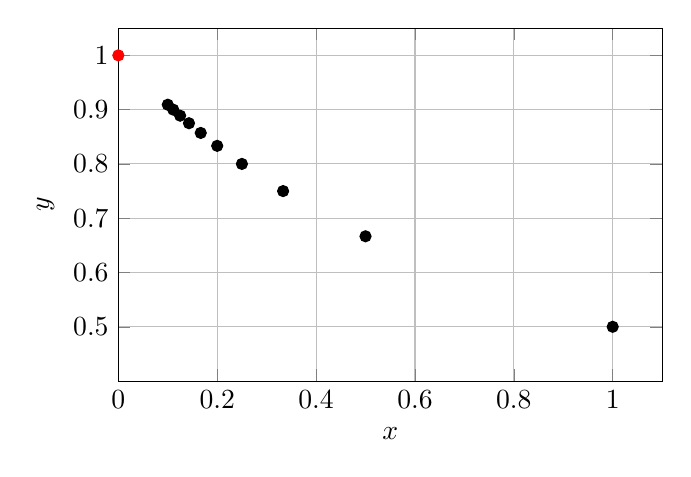
\begin{tikzpicture}
        \begin{axis}[
                xlabel={$x$},
                ylabel={$y$},
                xmin=0, xmax=1.1,
                ymin=0.4, ymax=1.05,
                xtick={0,0.2,0.4,0.6,0.8,1.0},
                ytick={0.5,0.6,0.7,0.8,0.9,1.0},
                grid=both,
                width=0.7\linewidth,
                height=0.5\linewidth
            ]
            % Punti della successione (approssimati in decimale)
            \addplot[only marks, mark=*] coordinates {
                (1.0,0.5)
                (0.5,0.6667)
                (0.3333,0.75)
                (0.25,0.8)
                (0.2,0.8333)
                (0.1667,0.8571)
                (0.1429,0.875)
                (0.125,0.8889)
                (0.1111,0.9)
                (0.1,0.9091)
            };
            % Evidenziamo il punto limite (0,1)
            \addplot[only marks, mark=*, red, mark size=2pt] coordinates {(0,1)};
            \node[red, below left] at (axis cs:0,1) {$(0,1)$};
        \end{axis}
    \end{tikzpicture}
    \end{center}
\end{exmp}

\vspace{10pt}

\paragraph{Punto interno}
\begin{bxthm}
\begin{defn}
    Siano $A\subseteq\mathbb{R}^n$ e $\overline{\mathbf{x}}\in A$. 
    Si dice che $\overline{\mathbf{x}}$ è \textbf{interno} ad $A$ se 
    \[\exists\,C\in\mathcal{C}_{\overline{\mathbf{x}}}\,:\;C\subseteq A.\]
\end{defn}
\end{bxthm}

\vspace{10pt}

I punti appartenenti al bordo del rettangolo non sono punti interni, poiché non esiste alcun cerchio con centro in un punto del bordo che sia interamente contenuto nel rettangolo. 
Al contrario, tutti i punti del rettangolo che non appartengono al bordo, sono punti interni, in quanto per ciascuno di essi è sempre possibile trovare un cerchio centrato nel punto stesso e 
completamente incluso nel rettangolo.
%fai disegno 

\vspace{10pt}

\begin{bxthm}
\begin{prop}
    Siano $A\subseteq\mathbb{R}^n$ e $\overline{\mathbf{x}}\in A$.
    Allora $\overline{\mathbf{x}}$ è interno ad $A$ se e solo se esiste un rettangolo di centro $\overline{\mathbf{x}}$ tale che $I\subseteq A$.
\end{prop}
\end{bxthm}
%\begin{proof}\hfill
%    \begin{itemize}
%        \item[$\implies$]
%        Per ipotesi, $\overline{\mathbf{x}}$ è interno ad $A$. Quindi 
%        \[\exists\,C\in\mathcal{C}_{\overline{\mathbf{x}}}\,:\;C\subseteq A.\]
%        Allora esiste un rettangolo $I$ di $\mathbb{R}^n$ di centro $\overline{\mathbf{x}}$ tale che $I\subseteq C$. 
%        Poichè $C\subseteq A$, anche $I\subseteq A$.
%        \item[$\impliedby$] 
%        Per ipotesi, esiste un rettangolo $I$ di centro $\overline{\mathbf{x}}$ tale che $I\subseteq A$. 
%        Allora \[\exists\,C\in\mathcal{C}_{\overline{\mathbf{x}}}\,:\;C\subseteq I.\]
%        Poichè $I\subseteq A$, anche $C\subseteq A$. Allora $\overline{\mathbf{x}}$ è interno ad $A$.
%    \end{itemize}
%\end{proof}

\vspace{10pt}

\paragraph{Interno di un insieme}
\begin{bxthm}
\begin{defn}
    L'insieme dei punti interni ad $A$ si chiama \textbf{interno} di $A$ e si indica con $\dot{A}$ 
\end{defn}
\end{bxthm}

\vspace{10pt}

\paragraph{Insieme aperto}
\begin{bxthm}
\begin{defn}
    Diciamo che un insieme $A\subseteq\mathbb{R}^n$ è \textbf{aperto} se $A=\dot{A}$.
\end{defn}
\end{bxthm}

\vspace{10pt}

\begin{bxthm}
    \begin{prop}
    Un insieme $A\subseteq\mathbb{R}^n$ è aperto se e solo se ogni punto di $A$ è interno ad $A$.
    \end{prop}
\end{bxthm}
%\begin{proof}\hfill
%\begin{itemize}
%    \item[$\implies$] Se $A$ è aperto, per definizione si ha $A=\dot{A}$; dunque ogni punto di $A$ è interno ad $A$.
%    \item[$\impliedby$] Se ogni punto di $A$ è interno ad $A$, cioè $A\subseteq\dot{A}$, e poiché per definizione $\dot{A}\subseteq A$, ne consegue che $A=\dot{A}$. Perciò, $A$ è aperto.
%\end{itemize}
%\end{proof}

\vspace{10pt}

\begin{exmp}
    $A=\{(x,y)\in\mathbb{R}^2\,:\; x>0\land y>0\}$
    $\dot{A}=A$, $A$ è aperto perchè tutti i punti di $A$ sono interni ad $A$.
\end{exmp}

\vspace{10pt}

\paragraph{Punto di frontiera}
\begin{bxthm}
\begin{defn}
    Siano $A\subseteq\mathbb{R}^n$ e $\overline{\mathbf{x}}\in\mathbb{R}^n$.
    Allora si dice che $\overline{\mathbf{x}}$ è un punto di \textbf{frontiera} per $A$ se per ogni cerchio 
    di $\overline{\mathbf{x}}$, esistono sia punti di $A$ sia punti non appartenenti ad $A$.
    In simboli:
    \[
    \forall\, C\in\mathcal{C}_{\overline{\mathbf{x}}},\quad C\cap A\neq\emptyset \quad \land \quad C\cap (\mathbb{R}^n\setminus A)\neq\emptyset.
    \]
\end{defn}
\end{bxthm}

\vspace{10pt}

\begin{exmp}
    Tutti i punti sul bordo di un rettangolo sono di frontiera perchè in ogni cerchio di centro un punto del bordo ci sono sia punti del rettangolo sia punti non appartenenti al rettangolo.
\end{exmp}

\vspace{10pt}

\begin{exmp}
    Consideriamo l'insieme
    \[ A=\{(x,y)\in\mathbb{R}^2 : x>0 \ \text{e} \ y>0\}, \]
    allora i punti appartenenti al semiasse definito da \(x>0\) e quelli appartenenti al semiasse definito da \(y>0\) costituiscono punti di frontiera per \(A\). 
    Infatti, per ogni punto di tali semiasse, ogni cerchio (ossia, ogni cerchio centrato in quel punto) interseca sia l'insieme \(A\) sia il suo complementare.
\end{exmp}

\vspace{10pt}

\paragraph{Frontiera di un insieme}
\begin{bxthm}
\begin{defn}
    L'insieme dei punti di frontiera per $A$ è detto \textbf{frontiera} di $A$ e si indica con $\textup{Fr}(A)$ o $\partial A$.
\end{defn}
\end{bxthm}

\vspace{10pt}

\begin{exmp}
    Per quanto riguarda un segmento chiuso \( A = [a,b] \subset \mathbb{R} \) (inteso come sottoinsieme dei reali), ogni punto del segmento risulta essere di frontiera, cioè
    \[
    \partial A = A.
    \]
\end{exmp}

\vspace{10pt}

\begin{exmp}
    Infine, considerando il primo quadrante
    \[
    A = \{(x,y) \in \mathbb{R}^2 : x>0 \text{ e } y>0\},
    \]
    la frontiera di \( A \) coincide con l'unione dei due semiasse positivi, formalmente espressa come
    \[
    \partial A = \{(x,0) : x > 0\} \cup \{(0,y) : y > 0\}.
    \]
\end{exmp}

\vspace{10pt}

\paragraph{Chiusura di un insieme}
\begin{bxthm}
\begin{defn}
    Si chiama \textbf{chiusura} di $A\subseteq\mathbb{R}^n$ l'insieme $\overline{A}=A\cup\partial A$. 
\end{defn}
\end{bxthm}

\vspace{10pt}

\paragraph{Insieme chiuso}
\begin{bxthm}
\begin{defn}
    Diciamo che un insieme $A\subseteq\mathbb{R}^n$ è \textbf{chiuso} se $A=\overline{A}$.
\end{defn}
\end{bxthm}

\vspace{10pt}

\begin{bxthm}
\begin{prop}
    Sia $A\subseteq\mathbb{R}^n$.
    Allora 
    \[A=\overline{A}\iff\forall\,x\in\overline{A},\;x\in A.\]
    o alternativamente
    \[A=\overline{A}\iff\overline{A}\subseteq A.\]
\end{prop}
\end{bxthm}
%\begin{proof}
%    Da
%    \[\overline{A}=A\cup\partial A,\]
%    segue che 
%    \[A=\overline{A}\iff A=A\cup \partial A \iff\partial A\subseteq A.\]
%\end{proof}

\vspace{10pt}

\begin{exmp}
Consideriamo i seguenti due insiemi in $\mathbb{R}^2$:
\begin{enumerate}
    \item Sia 
    \[
    A = [a,b] \times [c,d], \quad a,b,c,d\in\mathbb{R},\; a<b,\; c<d.
    \]
    Poiché per definizione l'intervallo chiuso $[a,b]$ contiene i suoi estremi, si ha
    \[
    \partial A \subset A,
    \]
    ovvero ogni punto di frontiera di $A$ appartiene ad $A$. Pertanto
    \[
    \overline{A} = A \quad \text{e } A \text{ è chiuso.}
    \]

    \item Sia
    \[
    B = \{(x,y)\in\mathbb{R}^2 : x>0 \text{ e } y>0\},
    \]
    che rappresenta il primo quadrante aperto. L'insieme dei punti di frontiera di $B$ è
    \[
    \partial B = \{(x,0) : x>0\}\cup\{(0,y) : y>0\}.
    \]
    Poichè nessun punto di $\partial B$ appartiene a $B$, si ha
    \[
    \partial B \not\subset B \quad \implies \quad \overline{B} = B\cup \partial B \neq B.
    \]
    Di conseguenza, l'insieme $B$ non è chiuso.
\end{enumerate}
\end{exmp}

\vspace{10pt}

Un altro concetto che ci serve è quello di punto di accumulazione e quello di punto isolato. 

\vspace{10pt}

\paragraph{Punto di accumulazione e punto isolato}
\begin{bxthm}
\begin{defn}
    Siano $A\subseteq\mathbb{R}^n$ e $\overline{\mathbf{x}}\in\mathbb{R}^n$. Diciamo che $\overline{\mathbf{x}}$ 
    è un \textbf{punto di accumulazione} per $A$ se \[\forall\,C\in\mathcal{C}_{\overline{\mathbf{x}}},\;A\cap C\setminus\{\overline{\mathbf{x}}\}\neq\emptyset.\]
    L'insieme dei punti di accumulazione si indica con \[\mathcal{D}(A)=\{\overline{\mathbf{x}}\in\mathbb{R}^n \ | \ \overline{\mathbf{x}} \textup{ è di accumulazione per }A\,\}.\]
    Se $\overline{\mathbf{x}}\in A$ non è di accumulazione per $A$, cioè se 
    \[\exists\,C\in\mathcal{C}_{\overline{\mathbf{x}}}\,:\;A\cap C=\{\overline{\mathbf{x}}\} \quad (\textup{o }A\cap C\setminus\{\overline{\mathbf{x}}\}=\emptyset), \]
    allora si dice che $\overline{\mathbf{x}}$ è \textbf{isolato}.
\end{defn}
\end{bxthm}

\vspace{10pt}

\begin{bxthm}
\begin{prop}
    Siano $A\subseteq\mathbb{R}^n$ e $\overline{\mathbf{x}}\in\mathbb{R}^n$.
    Allora $\overline{\mathbf{x}}\in\mathcal{D}(A)$ se e solo se $\forall\,C\in\mathcal{C}_{\overline{\mathbf{x}}}$, 
    esistono infiniti punti di $A$.
\end{prop}
\end{bxthm}

\vspace{10pt}

\begin{exmp}
    Consideriamo un cerchio nel piano. In esso, ogni punto del cerchio è un punto di accumulazione, sia che esso si trovi sul bordo sia che esso sia interno al cerchio. 
    Allo stesso modo, in un segmento ogni punto è di accumulazione. 
    Infine, nel caso del primo quadrante, i punti interni così come quelli appartenenti al bordo costituiscono punti di accumulazione.
\end{exmp}

\vspace{10pt}

\begin{bxthm}
\begin{prop}\hfill
    \begin{enumerate}
        \item $A\textup{ è chiuso}\iff\forall\,\mathbf{x}\in\mathcal{D}(A),\;\mathbf{x}\in A\;(\iff\mathcal{D}(A)\subseteq A)$;
        \item $\overline{\mathbf{x}}\in\partial A\,\cancel{\implies}\,\overline{\mathbf{x}}\in\mathcal{D}(A)$;
        \item $\overline{\mathbf{x}}\in\mathcal{D}(A)\,\cancel{\implies}\,\overline{\mathbf{x}}\in\partial A$.
    \end{enumerate}
\end{prop}
\end{bxthm}

\vspace{10pt}

\begin{rem}
Consideriamo due casi:
\begin{enumerate}
    \item \textbf{Il caso del rettangolo.}  
    Se $A$ è un rettangolo (cioè un prodotto di intervalli chiusi) in $\mathbb{R}^n$, ogni punto interno (cioè ogni punto che non appartiene al bordo) gode della proprietà che esiste un cerchio interamente contenuto in $A$.  
    In particolare, questo implica che:
    \begin{itemize}
        \item Ogni punto interno è un \textbf{punto di accumulazione} per $A$, poiché in ogni cerchio esso si trova insieme ad altri punti di $A$.
        \item Tuttavia, questi punti non sono punti di frontiera, perché non si ha l'intersezione dell'cerchio con $\mathbb{R}^n\setminus A$.
    \end{itemize}

    \item \textbf{Il caso degli isolati.}  
    Consideriamo l'insieme 
    \[
    A=\{(n,0)\,:\;n\in\mathbb{N}\}\subseteq\mathbb{R}^2.
    \]
    In questo insieme ogni punto $x_0=(n,0)$ è \textbf{isolato}, cioè esiste un cerchio $C\in\mathcal{C}_{(n,0)}$, con raggio sufficientemente piccolo da non includere né il punto precedente $(n-1,0)$ né il successivo $(n+1,0)$, tale che
    \[
    C\cap A=\{(n,0)\}.
    \]
    In questo caso:
    \begin{itemize}
        \item Poiché il punto è isolato, per definizione non può essere di accumulazione.
        \item Tuttavia, per ogni $n$, il punto $(n,0)$ appartiene comunque alla frontiera $\partial A$, poiché in ogni cerchio centrato in $(n,0)$ vi sono anche punti al di fuori di $A$. 
    \end{itemize}
\end{enumerate}

Questi esempi evidenziano alcune differenze chiave:
\begin{itemize}
    \item Un \textbf{punto interno} possiede intorni interamente contenuti in $A$ ed è automaticamente di accumulazione, ma non rientra nella frontiera.
    \item Un \textbf{punto di accumulazione} richiede che ogni cerchio contenga altri punti di $A$, mentre questo non implica che il punto sia di frontiera (dato che, se è interno, non si incontrano punti esterni).
    \item Un \textbf{punto isolato} è tale che esiste almeno un cerchio in cui non vi sono altri punti di $A$. Tali punti possono comunque appartenere alla frontiera, perché in ogni cerchio del punto si trovano anche punti di $\mathbb{R}^n\setminus A$, ma non sono di accumulazione.
\end{itemize}
\end{rem}

\vspace{10pt}

\begin{bxthm}
\begin{prop}
Sia $A\subseteq\mathbb{R}^n$. Allora $A$ è chiuso se e solo se per ogni successione $(x_k)_{k\in\mathbb{N}}$ tale che 
\[
    \forall\, k\in\mathbb{N},\;x_k\in A \quad \textup{ e } \quad \lim_{k\to+\infty} x_k = \mathbf{x},
\]
si ha che il limite $\mathbf{x}$ appartiene ad $A$. In altre parole, $A$ contiene tutti i limiti delle successioni di punti in $A$.
\end{prop}
\end{bxthm}

\vspace{10pt}

\paragraph{Insieme limitato}
\begin{bxthm}
\begin{defn}
    Si dice che $A\subseteq\mathbb{R}^n$ è \textbf{limitato} se $\exists$ un cerchio $C$ tale che $A\subseteq C$.    
\end{defn}
\end{bxthm}

\vspace{10pt}

\begin{bxthm}
\begin{prop}
    $A\subseteq\mathbb{R}^n$ è limitato se e solo se 
    \[\exists\, c>0 \,:\;\forall\,x\in A,\quad(\|x\|\leq c\;\textup{ e }\; \| x \|-\| \overline{\mathbf{x}} \|\leq \| x-\overline{\mathbf{x}} \|).\]
\end{prop}
\end{bxthm}
%\begin{proof}\hfill 
%    \begin{itemize}
%        \item[$\implies$] Dalle ipotesi esiste un cerchio $C$ tale che $A\subseteq C$. 
%        Sia $\overline{\mathbf{x}}$ il centro di $C$ e $r$ il suo raggio, avremo allora 
%        \[C_{\overline{\mathbf{x}}}(r)=\{x\in\mathbb{R}^n\,:\;\| x-\overline{\mathbf{x}} \|<r\}.\]
%        Poichè $A\subseteq C$, segue immediatamente che 
%        \[\forall\, x\in A,\quad \| x-\overline{\mathbf{x}} \|<r.\]
%        Dalla disuguaglianza triangolare 
%        \[\| x \| -\| \overline{\mathbf{x}} \|\leq\| x-\overline{\mathbf{x}} \|<r \implies \| x \|-\| \overline{\mathbf{x}} \|<r \implies \| x \|<\| \overline{\mathbf{x}} \|+r.\]
%        Ponendo $\| \overline{\mathbf{x}} \|+r=r$, ci troviamo con 
%        \[\forall x\in A, \| x \| < c.\]
%
%        \item[$\impliedby$] Dall'ipotesi si ha che esiste $c>0$ tale che
%        \[
%        \forall\, x\in A,\quad \|x\|\leq c.
%        \]
%        Consideriamo il cerchio chiuso centrato nell'origine di raggio $c$, definito da
%        \[
%        C_{0}(c)=\{x\in\mathbb{R}^n\,:\; \|x\|\leq c\}.
%        \]
%        Essendo che ogni elemento di $A$ ha norma minore o uguale a $c$, segue 
%        \[
%        A\subseteq C_{0}(c),
%        \]
%        cioè $A$ è limitato.
%    \end{itemize}
%\end{proof}

\vspace{10pt}

\begin{note}
    La prima parte della proposizione esprime la definizione classica di insieme limitato: esiste una costante $c>0$ tale che per ogni elemento $x\in A$ 
    la sua norma soddisfa $\|x\|\leq c$, cioè $A$ è contenuto in una palla centrata nell'origine di raggio $c$. La seconda disuguaglianza, 
    $\|x\|-\| \overline{\mathbf{x}} \|\leq \| x-\overline{\mathbf{x}} \|$, è una conseguenza della disuguaglianza triangolare (nella sua forma inversa) e indica che la 
    differenza tra la norma di $x$ e quella di un punto fisso $\overline{\mathbf{x}}$ è sempre minore o uguale alla distanza tra $x$ e $\overline{\mathbf{x}}$. 
    Questo fatto evidenzia come la "variazione" della norma, rispetto ad un punto fisso, sia controllata dalla distanza effettiva in $\mathbb{R}^n$. 
    Insieme, queste condizioni garantiscono che gli elementi di $A$ non "si allontanano" indefinitamente, cioè $A$ risulta limitato.
\end{note}

\vspace{10pt}

\paragraph{Insieme compatto}
\begin{bxthm}
\begin{defn}
    Si dice che $A\subseteq\mathbb{R}^n$ è \textbf{compatto} se è chiuso e limitato.
\end{defn}
\end{bxthm}

\vspace{10pt}

\paragraph{Insieme convesso}
\begin{bxthm}
\begin{defn}
    Si dice che $A\subseteq\mathbb{R}^n$ è \textbf{convesso} se 
    \[\forall\, \mathbf{x},\mathbf{y}\in A,\quad \overline{\mathbf{xy}}\subseteq A.\]
\end{defn}
\end{bxthm}

\vspace{10pt}

\paragraph{Insieme convesso per poligonali}
\begin{bxthm}
\begin{defn}
    Si dice che $A\subseteq\mathbb{R}^n$ è \textbf{convesso per poligonali} se per ogni coppia di punti 
    $\mathbf{x},\mathbf{y}$ di $A$ esiste una poligonale $P$ di estremi $\mathbf{x}$ e $\mathbf{y}$ tale che $P\subseteq A$.
\end{defn}
\end{bxthm}

\vspace{10pt}

\begin{note}
    Ogni insieme convesso possiede la proprietà che, per ogni coppia di punti al suo interno, il segmento che li unisce è contenuto in esso; pertanto, 
    essendo il segmento un caso particolare di poligonale, risulta che ogni insieme convesso è convesso per poligonale. 
    Tuttavia, la condizione inversa non è sempre verificata, come si nota nell'esempio della corona circolare, la quale ammette connessioni tramite 
    poligonali contenute nell'insieme pur non essendo convessa.
\end{note}

\vspace{10pt}

\paragraph{Insieme sconnesso}
\begin{bxthm}
\begin{defn}
    Si dice che $A\subseteq\mathbb{R}^n$ è \textbf{sconnesso} se esistono due insiemi aperti $A_1,A_2\subseteq\mathbb{R}^n$ tali che 
    \begin{enumerate}
        \item $A_1\cap A\neq\emptyset$ e $A_2\cap A\neq\emptyset$;
        \item $(A_1\cap A)\cap(A_2\cap A)=\emptyset$;
        \item $A=(A_1\cap A)\cup(A_2\cap A)$.
    \end{enumerate}
\end{defn}
\end{bxthm}

\vspace{10pt}

\paragraph{Insieme connesso}
\begin{bxthm}
\begin{defn}
    Si dice che $A\subseteq\mathbb{R}^n$ è \textbf{connesso} se non è sconnesso.
\end{defn}
\end{bxthm}

\vspace{10pt}

\begin{bxthm}
\begin{prop}
    Ogni insieme convesso per poligonale è anche connesso
\end{prop}
\end{bxthm}

\vspace{10pt}

\begin{bxthm}
\begin{prop}
   Sia $A\subseteq\mathbb{R}^n$ aperto.
   Allora $A$ è sconnesso se e solo se esistono due aperti $A_1$ e $A_2$ disgiunti e non vuoti tali che $A=A_1\cup A_2$.
\end{prop}
\end{bxthm}

\vspace{10pt}

\begin{bxthm}
\begin{thm}
    Sia $A\subseteq\mathbb{R}^n$ aperto.
    Allora $A$ è connesso se e solo se è convesso per poligonale.
\end{thm}
\end{bxthm}

\vspace{10pt}

Alla luce di quanto esposto, definiamo una funzione reale di due variabili come un'applicazione
\[
f: A \subseteq \mathbb{R}^2 \to \mathbb{R},\quad (x, y) \mapsto f(x, y).
\]
Analogamente, una funzione di tre variabili è data da
\[
f: A \subseteq \mathbb{R}^3 \to \mathbb{R},\quad (x, y, z) \mapsto f(x, y, z),
\]
mentre nel caso generale di una funzione di $n$ variabili si scrive
\[
f: A \subseteq \mathbb{R}^n \to \mathbb{R},\quad \mathbf{x} = (x_1, x_2, \dots, x_n) \mapsto f(x_1, x_2, \dots, x_n) = f(\mathbf{x}).
\]

\vspace{10pt}

% Esempi e osservazioni sulle funzioni e sui relativi grafici

% Esempio 1: Funzione in due variabili con dominio definito da un'inequazione lineare
Sia ad esempio 
\[
f(x,y)=\sqrt{\,y-x\,}.
\]
Per garantire il significato dell'espressione (cioè, che la radice quadrata sia definita nel campo dei numeri reali) è necessario richiedere
\[
y-x\ge 0 \quad\implies\quad y\ge x.
\]
Pertanto la funzione 
\[
f \colon A \subseteq \mathbb{R}^2 \to \mathbb{R}, \qquad f(x,y)=\sqrt{y-x},
\]
è definita sull'insieme
\[
A=\{(x,y)\in\mathbb{R}^2 \;:\; y\ge x\}\,.
\]

% Esempio 2: Funzione in due variabili con dominio definito da un'inequazione quadratica (relativa a una palla)
Sia invece 
\[
f(x,y)=\frac{1}{\sqrt{x^2+y^2-1}}\,.
\]
L'espressione sotto radice deve essere strettamente positiva; notiamo che
\[
x^2+y^2-1>0 \quad\implies\quad x^2+y^2>1\,.
\]
Quindi, la funzione è definita in
\[
A=\{(x,y)\in\mathbb{R}^2 \;:\; x^2+y^2>1\}\,,
\]
escludendo la frontiera del cerchio (ossia il luogo in cui \(x^2+y^2=1\)).


\paragraph{Grafico di una funzione di una variabile: funzione reale di una sola variabile}
% (il grafico risiede in R^2)
Sia \(f : I \subseteq \mathbb{R} \to \mathbb{R}\) una funzione di una sola variabile. Il grafico di \(f\) è definito dall'insieme
\[
G_f=\{(x,y)\in\mathbb{R}^2 \;:\; x\in I \text{ e } y=f(x)\}\,.
\]


\paragraph{Grafico di una funzione di due variabili: funzione reale di due variabili, grafico in $\mathbb{R}^3$}
Sia ora \(f : A \subseteq \mathbb{R}^2 \to \mathbb{R}\) una funzione di due variabili. Il relativo grafico è 
\[
G_f=\{(x,y,z)\in\mathbb{R}^3 \;:\; (x,y)\in A \text{ e } z=f(x,y)\}\,.
\]


\paragraph{Grafico in dimensione maggiore: funzione di $n$ variabili}
Generalmente, per una funzione \(f : A \subseteq \mathbb{R}^n \to \mathbb{R}\) (con
\[
f(x_1,x_2,\dots,x_n)=f(x)),
\]
il grafico di \(f\) è definito come
\[
G_f=\{(x_1,x_2,\dots,x_n,z)\in\mathbb{R}^{n+1} \;:\; x=(x_1,\dots,x_n)\in A \text{ e } z=f(x)\}\,.
\]
In particolare, quando \(f\colon \mathbb{R}^3\to\mathbb{R}\), il grafico \(G_f\) si considera un sottoinsieme di \(\mathbb{R}^4\).

\paragraph{Definizione formale di limite per una funzione di una variabile}
Sia \(f : I \subseteq \mathbb{R} \to \mathbb{R}\) una funzione e sia \(x_0\) un punto di accumulazione di \(I\). 
Si dice che 
\[
\lim_{x\to x_0}f(x)=l\in\mathbb{R}
\]
se
\[
\forall\,\varepsilon>0,\ \exists\,\delta>0 \text{ tale che } \forall\, x\in I \text{ con } 0<|x-x_0|<\delta,\quad |f(x)-l|<\varepsilon\,.
\]
In altre parole, per ogni cerchio di \(l\) (cioè, per ogni intervallo aperto centrato in \(l\) di ampiezza \(\varepsilon\)), si può trovare un cerchio di \(x_0\) (cioè un intervallo aperto centrato in \(x_0\) di raggio \(\delta\)) tale che ogni \(x\neq x_0\) in tale cerchio soddisfi \(f(x)\in (l-\varepsilon,l+\varepsilon)\).

Un'alternativa sintetica per esprimere la definizione è:
\[
\lim_{x\to x_0} f(x)=l \quad \iff \quad x\sim x_0,\;\implies f(x)\sim l\,.
\]
Questa espressione evidenzia il fatto che, avvicinandosi a \(x_0\), i valori di \(f\) si avvicinano ad \(l\).

\vspace{10pt}

\paragraph{Limite per una funzione a $n$ variabili}
\begin{bxthm}
\begin{defn}
    Siano $f:A\subseteq\mathbb{R}^n\to\mathbb{R}$ e $\overline{\mathbf{x}}\in\mathcal{D}(A)$. 
    Si dice che 
    \[\lim_{\mathbf{x}\to \overline{\mathbf{x}}}=l\in\mathbb{R}\]
    se 
    \[\forall\, \varepsilon>0\,,\; \exists\, \delta>0\,:\;\forall\, \mathbf{x}\in A,\quad 0<\| \mathbf{x}-\overline{\mathbf{x}} \|<\delta\implies | f(\mathbf{x})-l |<\varepsilon.\]
\end{defn}
\end{bxthm}

\vspace{10pt}

% Definizioni riguardanti il limite di una funzione

% La condizione 0 < \|x - x₀\| < δ significa che:
\[
0 < \|\mathbf{x}-\overline{\mathbf{x}}\| < \delta \quad \iff \quad \mathbf{x} \in C_{\overline{\mathbf{x}}}(\delta) \setminus \{\overline{\mathbf{x}}\},
\]
dove \(C_{\overline{\mathbf{x}}}(\delta)\) è un cerchio di centro \(\overline{\mathbf{x}}\) e raggio \(\delta\).

% Definizione del limite finito
Definiamo il limite di \(f\) in \(x_0\) nel seguente modo:
\[
\lim_{x\to x_0} f(x) = l \in \mathbb{R} \quad \iff \quad \forall\, J\in\mathcal{I}_l,\; \exists\, \delta > 0\,:\; \forall\, x \in A,\quad 0 < \|x - x_0\| < \delta\implies f(x) \in J.
\]
In altre parole, se \(x\) si avvicina a \(x_0\) (ovvero \(x \sim x_0\)), allora \(f(x)\) si avvicina a \(l\) (cioè \(f(x) \sim l\)).

% Definizione del limite infinito (positivo)
Si dice che
\[
\lim_{x\to x_0} f(x) = +\infty \quad \iff \quad \forall\, M > 0,\; \exists\, \delta > 0\,:\;\forall\, x \in A,\; 0 < \|x - x_0\| < \delta\implies f(x) > M.
\]

% Definizione del limite infinito (negativo)
Analogamente, si dice che
\[
\lim_{x\to x_0} f(x) = -\infty \quad \iff \quad \forall\, M < 0,\; \exists\, \delta > 0 \,:\; \forall\, x \in A,\; 0 < \|x - x_0\| < \delta\implies f(x) < M.
\]

\vspace{10pt}

\paragraph{Funzione continua in un punto}
\begin{bxthm}
\begin{defn}
    Sia $f:A\subseteq\mathbb{R}^n\to\mathbb{R}$ e sia $\overline{\mathbf{x}}\in A$. 
    Si dice che $f$ è \textbf{continua} in $\overline{\mathbf{x}}$ se 
    \[\forall\,\varepsilon>0,\;\exists\,\delta>0\,:\;\forall\, \mathbf{x}\in A,\quad\| \mathbf{x}-\overline{\mathbf{x}} \|<\delta \implies|f(\mathbf{x})-f(\overline{\mathbf{x}})|<\varepsilon.\]
    Alternativamente, 
    \[\forall\,\varepsilon>0,\;\exists\,C\in\mathcal{C}_{\overline{\mathbf{x}}}\,:\;\forall\, \mathbf{x}\in A\cap C,\quad|f(\mathbf{x})-f(\overline{\mathbf{x}})|<\varepsilon.\]
\end{defn}
\end{bxthm}

\vspace{10pt}

\begin{note}
$f$ è continua in $\overline{\mathbf{x}} \iff \forall\varepsilon>0,\;\exists\,C\in\mathcal{C}_{\overline{\mathbf{x}}}\,:\; 
\forall\, \mathbf{x}\in A\cap C, |f(\mathbf{x})-f(\overline{\mathbf{x}})|<\varepsilon.$
Se $\mathbf{x}\sim \overline{\mathbf{x}}$, $f(\mathbf{x})\sim f(\overline{\mathbf{x}})$
\end{note}

\vspace{10pt}

\begin{bxthm}
\begin{prop}\hfill
\begin{enumerate}
    \item Se $\overline{\mathbf{x}}$ è un punto isolato per $A$, ogni funzione è continua in $\overline{\mathbf{x}}$;
    \item Se $\overline{\mathbf{x}}\in\mathcal{D}(A)$, $f$ è continua in $\overline{\mathbf{x}} \iff \lim\limits_{\mathbf{x}\to \overline{\mathbf{x}}}f(\mathbf{x})=f(\overline{\mathbf{x}})$.
\end{enumerate}
\end{prop}
\end{bxthm}
%\begin{proof}\hfill 
%    \begin{enumerate}
%        \item Sia $\overline{\mathbf{x}}$ un punto isolato. Allora 
%        \[\exists\,\overline{C}\in\mathcal{C}_{\overline{\mathbf{x}}}\,:\;\overline{C}\cap A=\{\overline{\mathbf{x}}\}.\]
%        Siano $\varepsilon>0$ e  $C=\overline{C}$. Poichè $C\cap A=\{\overline{\mathbf{x}}\}$, avremo che $|f(\overline{\mathbf{x}})-f(\overline{\mathbf{x}})|=0<\varepsilon$.
%        \item Sia $\overline{\mathbf{x}}$ di accumulazione per $A$. Allora 
%        \[\lim_{\mathbf{x}\to \overline{\mathbf{x}}} f(\mathbf{x})=f(\overline{\mathbf{x}})\iff \forall\,\varepsilon>0,\;\exists\,\delta>0\,:\; \forall\, \mathbf{x}\in A,\quad 0<\|\mathbf{x}-\overline{\mathbf{x}}\|<\delta\implies |f(\mathbf{x})-f(\overline{\mathbf{x}})|<\varepsilon.\] 
%        La condizione $|f(\mathbf{x})-f(\overline{\mathbf{x}})|<\varepsilon$ vale $\forall\, \mathbf{x}\in A$ con $\| \mathbf{x}-\overline{\mathbf{x}} \|<\delta$, cioè $f$ è continua in $\overline{\mathbf{x}}$.
%    \end{enumerate}
%\end{proof}

\vspace{10pt}

\paragraph{Funzione continua}
\begin{bxthm}
\begin{defn}
    Si dice che $f$ è continua in $A$ se è continua in ogni punto di $A$.
    In simboli,
    \[\forall\, \overline{\mathbf{x}}\in A,\;\forall\,\varepsilon>0,\;\exists\,\delta>0\,:\;\forall\, \mathbf{x}\in A,\quad\| \mathbf{x}-\overline{\mathbf{x}} \|<\delta \implies|f(\mathbf{x})-f(\overline{\mathbf{x}})|<\varepsilon.\]
\end{defn}
\end{bxthm}

\vspace{10pt}

\paragraph{Funzione uniformemente continua}
\begin{bxthm}
\begin{defn}
    Si dice che $f$ è uniformemente continua in $A$ se 
    \[\forall\,\varepsilon>0,\;\exists\,\delta>0\,:\;\forall\, x,y\in A,\quad\| x-y \|<\delta\implies |f(x)-f(y)|<\varepsilon.\]
\end{defn}
\end{bxthm}

\vspace{10pt}

\begin{note}
    Questa definizione è più forte della normale continuità poichè la implica, mentre non è vero il contrario.
\end{note}

\vspace{10pt}

\paragraph{Teorema di Cantor}
\begin{bxthm}
\begin{thm}
    Sia $f:A\subseteq\mathbb{R}^n\to\mathbb{R}$ continua con $A$ compatto.
    Allora $f$ è uniformemente continua.
\end{thm}
\end{bxthm}

\vspace{10pt}

\paragraph{Teorema di Weierstrass}
\begin{bxthm}
\begin{thm}
    Sia $f:A\subseteq\mathbb{R}^n\to\mathbb{R}$ continua con $A$ compatto.
    Allora $f$ ha minimo e massimo. In simboli 
    \[\exists\,x_1,x_2\in A\,:\;\forall\, x\in A,\;f(x_1)\leq f(x)\leq f(x_2).\]
\end{thm}
\end{bxthm}

\vspace{10pt}

\paragraph{Teorema della permanenza del segno}
\begin{bxthm}
\begin{thm}
    Sia $f:A\subseteq\mathbb{R}^n\to\mathbb{R}$ continua con $f(\overline{\mathbf{x}})>0$. Allora 
    \[\exists\,C\in\mathcal{C}_{\overline{\mathbf{x}}}\,:\;\forall x\in A\cap C,\; f(x)>0.\]
\end{thm}
\end{bxthm}

\vspace{10pt}

\paragraph{Teorema dei valori intermedi}
\begin{bxthm}
\begin{thm}
    Sia $f:A\subseteq\mathbb{R}^n\to\mathbb{R}$ continua con $A$ limitato e connesso.
    Allora $f$ assume tutti i valori compresi tra l'estremo inferiore e l'estremo superiore.
    Cioè ponendo $m=\inf\{f(x):x\in A\}$ e $M=\sup\{f(x):x\in A\}$, avremo che 
    \[\forall\,\alpha\in\,]m,M[\,,\;\exists\,\overline{\mathbf{x}}\in A\,:\;f(\overline{\mathbf{x}})=\alpha.\]
\end{thm}
\end{bxthm}

\vspace{10pt}

\paragraph{Coordinate polari}
Fissiamo un'unità di misura per le lunghezze, una per gli angoli, e un verso di percorrenza per gli angoli.
Sia $P$ un punto nel piano diverso dal polo $P_0$.
Allora si definisce \textbf{modulo} $\rho$ di $P$ la lunghezza del segmento $\overline{P_0P}$, e 
\textbf{anomalia} $\theta$ di $P$ la misura dell'angolo che la semiretta $r$ forma con la semiretta $\overline{P_0P}$.
Chiamiamo $\rho$ e $\theta$ \textbf{coordinate polari} di $P$.
Se $P=P_0$, allora diciamo che il modulo è uguale a zero e l'anomalia non è definita.
$\rho$ ci dice che $P$ si trova nella circonferenza di centro $P_0$ e raggio $\rho$.

\paragraph{Passaggio da coordinate cartesiane a polari e viceversa}
Ci sono delle formule che permettono di passare dalle coordinate polari a quelle cartesiane e viceversa. 
Per ottenre queste formule prendiamo un riferimento cartesiano in cui la semiretta $r$ coincide con il semiasse $x$ positivo e quindi il polo $P_0$ coinciderà con l'origine delle coordinate.

Poichè $\rho$ è la lunghezza del segmento $\overline{P_0P}$, $\rho$ coincide con la distanza di $P$ da $(0,0)$. 
Se denotiamo con $x$ e $y$ le coordinate cartesiane del punto $P$, 
la distanza di $P$ dall'origine è $\rho=\sqrt{x^2+y^2}$.
Per le formule trigonometriche, abbiamo
\begin{equation}
    \begin{cases}
        x=\rho\cos \vartheta\\
        y=\rho\sin \vartheta
    \end{cases}\label{coord}  
\end{equation}
Se conosciamo $\rho$ e $\vartheta$, ci ricaviamo $x$ e $y$ da \ref{coord}. 
Viceversa, se conosciamo $x$ e $y$, seguirà $\rho=\sqrt{x^2+y^2}$ e da \ref{coord} 
\[\cos v=\dfrac{x}{\rho}\quad \sin x=\dfrac{y}{\rho}.\]

\vspace{10pt}

\begin{exmp}
    Sia $P=(1,1)$. Allora $\rho=\sqrt{1^2+1^2}=\sqrt{2}$. Da cui 
    \[\begin{cases}
        x=\rho\cos\vartheta\\
        y=\rho\sin\vartheta
    \end{cases}=\begin{cases}
        1=\sqrt{2}\cos\vartheta\\
        1=\sqrt{2}\sin\vartheta
    \end{cases}\implies \cos\vartheta=\dfrac{\sqrt{2}}{2}=\sin\vartheta\implies \vartheta=\dfrac{\pi}{4}.\]
    Sia $P=(2,\frac{\pi}{3})$.
\end{exmp}

\vspace{10pt}

\paragraph{Caso in cui $P_0\neq(0,0)$}
Prendiamo un riferimento cartesiano in cui la semiretta $r$ sia parallela al semiasse $x$ positivo, e $P_0=(x_0,y_0)\neq(0,0)$.
Dato un $P(x,y)\neq P_0$, avremo che $\rho=\sqrt{(x-x_0)^2+(y-y_0)^2}$, dunque 
\[\begin{cases}
        x-x_0=\rho\cos\vartheta\\
        y-y_0=\rho\sin\vartheta
    \end{cases}=\begin{cases}
        x=\rho\cos\vartheta+x_0\\
        y=\rho\sin\vartheta+y_0
    \end{cases}.\]

\vspace{10pt}

Ogni volta che si assegna un valore a una variabile in una funzione a due variabili, si ottiene una funzione che dipende solo dall'altra variabile (l'altra è diventata un parametro) rispetto a un punto fisso.
Ad esempio, data $f(x,y)=\sqrt{x^2+y^2}$, troviamo che per $y=1$, abbiamo $f(x)={x^2+1}$.
Questo ci permette di introdurre le funzioni parziali.

\vspace{10pt}

\paragraph{Funzioni parziali}
\begin{bxthm}
\begin{defn}\label{funzparz}
    Siano $f:A\subseteq\mathbb{R}^2\to\mathbb{R}$ e $(x_0,y_0)\in\mathbb{R}^2$.
    Definiamo le seguenti \[\varphi :x\to f(x,y_0)\quad\psi :y\to f(x_0,y).\]
    $\varphi$ e $\psi$ si chiamano \textbf{funzioni parziali} generate da $f$ rispetto a $(x_0,y_0)$.
    Geometricamente, $\varphi\;(\psi)$  può essere vista come $f$ calcolata lungo la retta $y=y_0\;(x=x_0)$.
    %Aggiungere quì disegno sulle note
    Non è detto che $\varphi$ e $\psi$ siano ben definiti.
    $\varphi$ è definita in \[A_\varphi=\{x\,|\,(x,y_0)\in A\},\] mentre $\psi$ è definita in \[A_\psi=\{y\,|\,(x_0,y)\in A\}.\]
    Inoltre, 
    \[(x_0,y_0)\in A\implies x_0\in A_\varphi\;\land\;y_0\in A_\psi.\]
\end{defn}
\end{bxthm}

\vspace{10pt}

\begin{bxthm}
\begin{thm}
    Se $(x_0,y_0)$ è interno ad $A$, allora $x_0$ è interno ad $A_\varphi$ e $y_0$ è interno ad $A_\psi$.
    In simboli:
    \[(x_0,y_0)\in\dot{A}\implies\exists\, r>0\,:\;[x_0-r,x_0+r]\subseteq A_\varphi\;\land\;[y_0-r,y_0+r]\subseteq A_\psi.\]
\end{thm}
\end{bxthm}
%\begin{proof}
%    Poichè $(x_0,y_0)\in\dot{A}$, $\exists$ un cerchio $C$ di centro $(x_0,y_0)$ tale che $C\subseteq A$. Sia $r$ il raggio di $C$.
%    Dimostriamo che $[x_0-r,x_0+r]\subseteq A_\varphi$. 
%    Da $x\in [x_0-r,x_0+r]$ abbiamo $|x-x_0|\leq r$.
%    Dimostriamo che $(x,y_0)\in C$.
%    \[\| (x,y_0)-(x_0,y_0) \|=\| (x-x_0,0) \|=\sqrt{(x-x_0)^2}=|x-x_0|\leq r\implies (x,y_0)\in C.\]
%    Poichè $C\subseteq A$, avremo che $(x,y_0)\in A$ da cui $x\in A_\varphi$.
%    In maniera analoga si dimostra che $[y_0-r,y_0+r]\subseteq A_\psi$.
%\end{proof}

\vspace{10pt}

\begin{note}
    Se $(x_0,y_0)\in \partial A$, $\varphi$ e $\psi$ potrebbero essere definite solo in un punto.
    Siano ad esempio
    \[A=C_{(0,0)}(1),\quad (x_0,y_0)=(0,1),\quad \varphi(x)=f(x,1).\]
    I punti $(x,1)$ sono i punti della retta $y=1$, che incontra $A$ solo nel punto $(0,1)$.
    %fare disegno
\end{note}

\vspace{10pt}

\paragraph{Teorema sui limiti delle funzioni parziali}
\begin{bxthm}
\begin{thm}
    Siano $f:A\subseteq\mathbb{R}^2\to\mathbb{R}$ e $(x_0,y_0)\in\mathcal{D}(A)$.
    Supponiamo che 
    \[\lim_{(x,y)\to(x_0,y_0)}f(x,y)=l\in\overline{\mathbb{R}}.\]
    Allora 
    \[x_0\in\mathcal{D}(A_\varphi)\implies \lim_{x\to x_0}\varphi(x)=l\quad\land\quad y_0\in\mathcal{D}(A_\psi)\implies \lim_{y\to y_0}\psi(y)=l.\]
\end{thm}
\end{bxthm}
%\begin{proof}
%    Sia $l\in\mathbb{R}$, per $\pm\infty$ la dimostrazione è analoga. 
%    Sia $x_0\in\mathcal{D}(A_\varphi)$. Vogliamo dimostrare che $\lim\limits_{x\to x_0}\varphi(x)=l$,
%    cioè che
%    \[\forall\,\varepsilon>0,\;\exists\,\delta>0\,:\;\forall\, x\in A_\varphi,\quad 0<|x-x_0|<\delta\implies|\varphi(x)-l|<\varepsilon.\]
%    Per ipotesi, 
%    \[\forall\,\varepsilon>0,\;\exists\,\delta>0\,:\;\forall\,(x,y)\in A,\quad 0<\|(x,y)-(x_0,y_0)\|<\delta\implies|f(x,y)-l|<\varepsilon.\]
%    Prendiamo $\varepsilon>0$ e $\delta$ come nell'ipotesi. 
%    Sia $x\in A_\varphi$ con $0<|x-x_0|<\delta$ e ricordiamo che $x\in A_\varphi\implies(x,y_0)\in A$.
%    Abbiamo dunque 
%    \[\| (x,y_0)-(x_0,y_0) \|=\|(x-x_0)\|=\sqrt{(x-x_0)^2}=|x-x_0|\implies 0<\|(x,y)-(x_0,y_0)\|<\delta.\]
%    In conclusione,
%    \[((x,y_0)\in A \;\land\; 0<\| (x,y)-(x_0,y_0) \|<\delta)\implies |f(x,y_0)-l|<\varepsilon\implies |\varphi(x)-l|<\varepsilon\implies f(x,y_0)=\varphi(x).\]
%\end{proof}

\vspace{10pt}

Il teorema dice che se $f$ ha un limite $l$ in un punto $(x_0,y_0)$, $f$ ha lo stesso limite lungo la retta $y=y_0$ e lungo la retta $x=x_0$.
Segue ovviamente che 
\[\lim_{x\to x_0}\varphi(x)\neq\lim_{y\to y_0}\psi(y)\implies\nexists\lim_{(x,y)\to(x_0,y_0)}f(x,y).\]

\vspace{10pt}

\begin{exmp}
    Sia ad esempio la seguente funzione 
    \[f:A=\mathbb{R}^2\setminus\{(0,0)\}\to\mathbb{R},\quad (x,y)\mapsto\dfrac{x^2}{x^2+y^2}.\]
    \begin{center}
        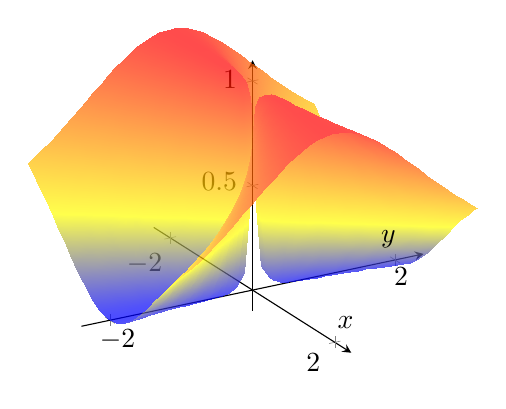
\begin{tikzpicture}
            \begin{axis}[
                view={60}{30}, % Angolazione della vista
                axis lines=center,
                xlabel={$x$},
                ylabel={$y$},
                domain=-2:2,
                y domain=-2:2,
                samples=40,
                samples y=40,
                enlargelimits=true,
                colormap/hot
            ]
                \addplot3[
                    surf,
                    shader=interp,
                    opacity=0.7,
                ]
                {x^2/(x^2 + y^2)};
            \end{axis}
        \end{tikzpicture}
        \hspace{1cm}
        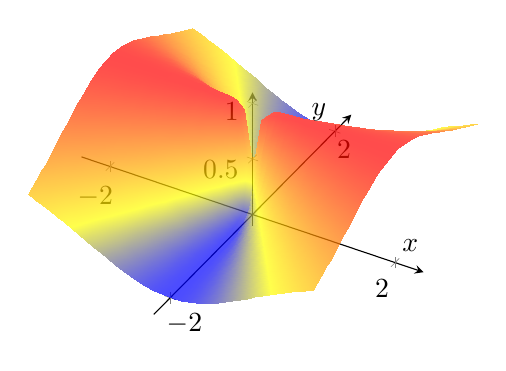
\begin{tikzpicture}
            \begin{axis}[
                view={30}{60}, % Angolazione della vista
                axis lines=center,
                xlabel={$x$},
                ylabel={$y$},
                domain=-2:2,
                y domain=-2:2,
                samples=40,
                samples y=40,
                enlargelimits=true,
                colormap/hot
            ]
                \addplot3[
                    surf,
                    shader=interp,
                    opacity=0.7,
                ]
                {x^2/(x^2 + y^2)};
            \end{axis}
        \end{tikzpicture}
    \end{center}
    Abbiamo che $(0,0)\in\mathcal{D}(A)$.
    Calcoliamo i limiti delle funzioni parziali nell'origine: 
    \[\varphi(x)=f(x,0)=\dfrac{x^2}{x^2+0}=\dfrac{x^2}{x^2}=1,\quad\psi(y)=f(0,y)=\dfrac{0}{0+y^2}=0,\]
    i due limiti differiscono, dunque possiamo concludere che $\nexists\lim_{(x,y)\to(0,0)}f(x,y)$.
\end{exmp}

\vspace{10pt}

Non vale però il viceversa del teorema, cioè se $\lim\limits_{x\to x_0}\varphi(x)=\lim\limits_{y\to y_0}\psi(y)$, non possiamo concludere che $\exists\lim_{(x,y)\to(x_0,y_0)}f(x,y)$.

\vspace{10pt}

\begin{exmp} 
    Sia ad esempio la seguente funzione 
    \[f:A=\mathbb{R}^2\setminus\{(0,0)\}\to\mathbb{R},\quad (x,y)\mapsto\dfrac{xy}{x^2+y^2}.\]
    \begin{center}
        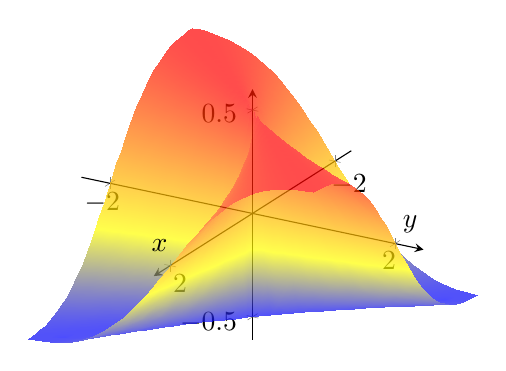
\begin{tikzpicture}
            \begin{axis}[
                view={120}{30}, % Angolazione della vista
                axis lines=center,
                xlabel={$x$},
                ylabel={$y$},
                domain=-2:2,
                y domain=-2:2,
                samples=40,
                samples y=40,
                enlargelimits=true,
                colormap/hot
            ]
                \addplot3[
                    surf,
                    shader=interp,
                    opacity=0.7,
                ]
                {x*y/(x^2 + y^2)};
            \end{axis}
        \end{tikzpicture}
        \hspace{1cm}
        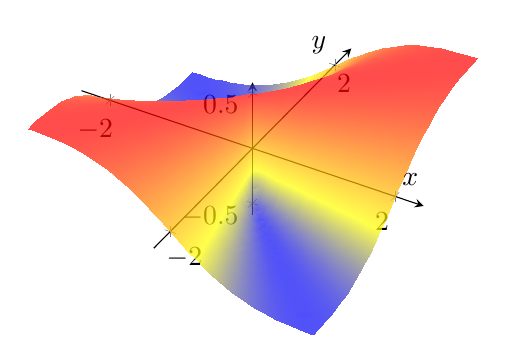
\begin{tikzpicture}
            \begin{axis}[
                view={30}{60}, % Angolazione della vista
                axis lines=center,
                xlabel={$x$},
                ylabel={$y$},
                domain=-2:2,
                y domain=-2:2,
                samples=40,
                samples y=40,
                enlargelimits=true,
                colormap/hot
            ]
                \addplot3[
                    surf,
                    shader=interp,
                    opacity=0.7,
                ]
                {x*y/(x^2 + y^2)};
            \end{axis}
        \end{tikzpicture}
    \end{center}
    Calcoliamo i limiti delle funzioni parziali nell'origine: 
    \[\varphi(x)=f(x,0)=\dfrac{x\cdot0}{x^2+0}=0,\quad\psi(y)=f(0,y)=\dfrac{0\cdot y}{0+y^2}=0,\]
    $\varphi$ e $\psi$ sono definite in $\mathbb{R}\setminus\{0\}$ e hanno limite $0$ in $0$, dunque secondo il teorema precedente dovremo avere $\lim_{(x,y)\to(0,0)}\dfrac{xy}{x^2+y^2}=0$, ma non è così perchè il limite non esiste.
    Dire che 
    \[\lim_{(x,y)\to(0,0)}\dfrac{xy}{x^2+y^2}=0\]
    equivale a dire che 
    \[\forall\,\varepsilon>0,\;\exists\,C\in\mathcal{C}_{(0,0)}\,:\;\forall\,(x,y)\in C\cap A\setminus\{(0,0)\},\quad\left|\dfrac{xy}{x^2+y^2}\right|<\varepsilon.\]
    Per dimostrare che 
    \[\lim_{(x,y)\to(0,0)}\dfrac{xy}{x^2+y^2}\neq0,\]
    dobbiamo negare la proposizione sudetta, ossia dimostrare che
    \[\exists\,\varepsilon>0\,:\;\forall\, C\in\mathcal{C}_{(0,0)},\; \exists\,(x,y)\in C\cap A\setminus\{(0,0)\}\,:\;\left|\dfrac{xy}{x^2+y^2}\right|\geq\varepsilon.\]
    Sulla bisettrice $y=x$, $f$ diventa $\dfrac{x^2}{x^2+x^2}=\dfrac{1}{2}$. In ogni cerchio di centro $(0,0)$, esistono punti della bisettrice in cui $f=\frac{1}{2}$.
    Sia $0<\varepsilon\leq\dfrac{1}{2}$. Se $C$ è un cerchio di centro $(0,0)$, in $C$ $\exists$ punti in cui $f=\dfrac{1}{2}\geq\varepsilon$
    \[\implies\lim_{(x,y)\to(0,0)}\neq0\implies\nexists\lim_{(x,y)\to(0,0)}\dfrac{xy}{x^2+y^2}.\]
\end{exmp}

\vspace{10pt}

\begin{bxthm}
\begin{cor}
Se $f:A\subseteq\mathbb{R}^2\to\mathbb{R}$ è continua in un punto $(x_0,y_0)\in A$, allora $\varphi$ è continua in $x_0$ e $\psi$ è continua in $y_0$.
\end{cor}
\end{bxthm}
%\begin{proof}
%    Come primo passo, dimostriamo che se $(x_0,y_0)$ è isolato per $A$, allora $x_0$ è isolato per $A_\varphi$ e $y_0$ è isolato per $A_\psi$.
%    Se $(x_0,y_0)$ è isolato per $A$, allora $\exists\,C\in\mathcal{C}_{(x_0,y_0)}\,:\;C\cap A=\{(x_0,y_0)\}$.
%    Sia dunque $r$ il raggio di $C$.
%    Dal teorema abbiamo che 
%    \[[x_0-r,x_0+r]\cap A_\varphi=\{x_0\}\quad\land\quad[y_0-r,y_0+r]\cap A_\psi=\{y_0\},\]
%    da cui possiamo estrarre
%    \[\{x_0\}\subseteq[x_0-r,x_0+r]\cap A_\varphi.\]
%    Sia ora $x\in[x_0-r,x_0+r]\cap A_\varphi$, da \ref{funzparz} sappiamo che $x\in A_\varphi\implies(x,y_0)\in A$.
%    Poichè $x\in[x_0-r,x_0+r]$, avremo che $\| (x,y_0)-(x_0,y_0) \|=\|(x-x_0,0)\|=|x-x_0|\leq r$.
%    Dunque $(x,y_0)\in C\implies x=x_0$.
%    %\[\| (x,y_0)-(x_0,y_0) \|=|x-x_0|\leq r\implies (x,y_0)\in C. (x,y_0)\in C\cap A=\{(x_0,y_0)\}\implies x=x_0.\]
%\end{proof}

\vspace{10pt}

\paragraph{Funzione separatamente continua}
\begin{bxthm}
\begin{defn}
Se $\varphi$ è continua in $x_0$ e $\psi$ è continua in $y_0$, si dice che $f$ è \textbf{separatamente continua} in $(x_0,y_0)$.    
\end{defn}
\end{bxthm}

\vspace{10pt}

\begin{note}
    Dunque se $f$ è continua in $(x_0,y_0)$, allora è anche separatamente continua in $(x_0,y_0)$, mentre il viceversa non vale.
\end{note}

\vspace{10pt}

\begin{exmp}
Sia ad esempio 
\[f:A\subseteq\mathbb{R}^2\to\mathbb{R},\quad (x,y)\mapsto\begin{cases}
    \frac{xy}{x^2+y^2}\quad (x,y)\neq(0,0)\\
    0\quad (x,y)=(0,0)
\end{cases}.\]
Poichè \(\varphi(x)=f(x,0)=0\) e  \(\psi(y)=f(0,y)=0\), abbiamo che 
$\varphi$ e $\psi$ sono continue in $0$, ma $f$ non è continua in $(0,0)$ perchè 
\[\nexists\lim_{(x,y)\to(0,0)}\dfrac{xy}{x^2+y^2}.\]
\end{exmp}

\vspace{10pt}

\begin{rem}
    Se $x_0$ è un punto isolato per $A_\varphi$, $\varphi$ è continua in $x_0$. 
    Se $x_0$ è di accumulazione per $A_\varphi$, $(x_0,y_0)$ è di accumulazione per $A$ perchè, se $(x_0,y_0)$ fosse isolata per $A$, anche $x_0$ sarebbe isolato per $A_\varphi$.
    Allora, poichè $f$ è continua in $(x_0,y_0)$, avremo che \[\lim_{(x,y)\to(x_0,y_0)}f(x,y)=f(x_0,y_0).\]
    Quindi, per il teorema precedente, 
    \[\lim_{x\to x_0}\varphi(x)=f(x_0,y_0)\] con $\varphi(x)=f(x,y_0)$ dunque 
    \[\lim_{x\to x_0}\varphi(x)=f(x_0,y_0)=\varphi(x_0), \]
    e dunque $\varphi$ è continua in $x_0$.
    In maniera analoga si procede per $\psi$.
\end{rem}

\vspace{10pt}

\paragraph{Equazione del grafico e curve cartesiane}
\begin{bxthm}
\begin{defn}
    Se $\rho :I\subseteq\mathbb{R}\to\mathbb{R} $ è una funzione di una sola variabile, l'equazione 
    \[y=\rho(x)\]
    è l'\textbf{equazione del grafico} di $\rho$.
    \[G_\rho=\{(x,\rho(x))\,:\;x\in I\}.\]
    I grafici delle funzioni continue di una variabile si chiamano \textbf{curve cartesiane}. 
    Se $\rho :I\subseteq\mathbb{R}\to\mathbb{R}$, una curva cartesiana è $\{(x,\rho x):x\in I\}$.    
\end{defn}
\end{bxthm}

\vspace{10pt}

\paragraph{Teorema sui limiti lungo le curve}
\begin{bxthm}
\begin{prop}
Sia $f: A \subseteq \mathbb{R}^2 \to \mathbb{R}$ una funzione e sia $(x_0, y_0)$ un punto di accumulazione per l'insieme $A$. Supponiamo che il limite globale esista:
$$ \lim_{(x,y) \to (x_0,y_0)} f(x,y) = \ell \in \hat{\mathbb{R}} $$
Sia inoltre $\rho: I \to \mathbb{R}$ una funzione continua definita in un intervallo reale $I$ contenente $x_0$, tale che $\rho(x_0) = y_0$ e che mappi i punti dell'intervallo (escluso il centro) all'interno del dominio $A$, ovvero:
$$ \forall x \in I \setminus \{x_0\}, \quad (x, \rho(x)) \in A $$
Allora vale l'uguaglianza:
$$ \lim_{x \to x_0} f(x, \rho(x)) = \ell $$
\end{prop}
\end{bxthm}

\vspace{10pt}

Interpretazione geometrica: $y = \rho(x)$ rappresenta l'equazione del grafico della funzione $\rho$. Di conseguenza, l'espressione $f(x, \rho(x))$ rappresenta la funzione $f$ valutata lungo la curva cartesiana definita da tale equazione. Il teorema afferma che se il limite globale esiste, il limite calcolato lungo questa specifica curva deve coincidere con esso.

\vspace{10pt}

%\begin{proof}
%Consideriamo il caso in cui il limite sia finito, ovvero $\ell \in \mathbb{R}$.
%
%Per ipotesi, vale la definizione di limite per funzioni di due variabili:
%$$ \left[ \forall \varepsilon > 0, \exists \delta > 0 : \forall (x,y) \in A \text{ con } 0 < ||(x,y) - (x_0, y_0)|| < \delta , \implies |f(x,y) - \ell| < \varepsilon \right] \quad (\star) $$
%
%Vogliamo dimostrare la tesi (Th) per il limite in una variabile:
%$$ \forall \varepsilon > 0, \exists \delta' > 0 : \forall x \in I \setminus \{x_0\} \text{ con } |x - x_0| < \delta', \implies |f(x, \rho(x)) - \ell| < \varepsilon $$
%
%Fissiamo $\varepsilon > 0$ e prendiamo il $\delta$ fornito dall'ipotesi $(\star)$.
%Sfruttiamo ora la continuità della funzione $\rho$ nel punto $x_0$. Per definizione di continuità, esiste un $\overline{\delta} > 0$ tale che:
%$$ \forall x \in I \text{ con } |x - x_0| < \overline{\delta} \implies |\rho(x) - y_0| < \frac{\delta}{2} $$
%Scegliamo ora $\delta'$ come il minimo tra i due raggi individuati:
%$$ \delta' = \min \left\{ \overline{\delta}, \frac{\delta}{2} \right\} $$
%Sia $x \in I \setminus \{x_0\}$ tale che $|x - x_0| < \delta'$. Consideriamo il punto $(x, \rho(x))$.
%Per le ipotesi sulla funzione $\rho$, sappiamo che $(x, \rho(x)) \in A$.
%Valutiamo la distanza di questo punto da $(x_0, y_0)$:
%$$ ||(x, \rho(x)) - (x_0, y_0)|| = ||(x-x_0, \rho(x)-y_0)|| = \sqrt{(x-x_0)^2 + (\rho(x)-y_0)^2} $$
%Poiché $x \neq x_0$, il termine sotto radice è strettamente positivo:
%$$ \sqrt{(x-x_0)^2 + (\rho(x)-y_0)^2} > \sqrt{(x-x_0)^2} = |x-x_0| > 0 $$
%Inoltre, poiché $|x-x_0| < \delta' \le \frac{\delta}{2}$ e $|\rho(x)-y_0| < \frac{\delta}{2}$, la norma è limitata da $\delta$.
%
%Riassumendo, se $x \in I \setminus \{x_0\}$ e $|x-x_0| < \delta'$, allora il punto $(x, \rho(x))$ appartiene ad $A$ e soddisfa:
%$$ 0 < ||(x, \rho(x)) - (x_0, y_0)|| < \delta $$
%Ci troviamo quindi nelle condizioni per applicare l'ipotesi $(\star)$, da cui segue che:
%$$ |f(x, \rho(x)) - \ell| < \varepsilon $$
%Questo conclude la dimostrazione.
%\end{proof}

\vspace{10pt}

Analizziamo ora un metodo fondamentale per lo studio dei limiti: il passaggio alle coordinate polari.
Dato un limite per $(x,y) \to (x_0, y_0)$ di una funzione $f: A \subseteq \mathbb{R}^2 \to \mathbb{R}$, possiamo effettuare il seguente cambio di variabili:
$$ \begin{cases} x = x_0 + \rho \cos \theta \\ y = y_0 + \rho \sin \theta \end{cases} $$
dove $\rho = \sqrt{(x-x_0)^2 + (y-y_0)^2}$ rappresenta la distanza dal punto limite.

Possiamo definire una nuova funzione $F$ nelle variabili $\rho$ e $\theta$:
$$ F(\rho, \theta) = f(x_0 + \rho \cos \theta, y_0 + \rho \sin \theta) $$
$F$ rappresenta la funzione originale $f$ espressa (o trasformata) in coordinate polari.

\vspace{10pt}

\begin{exmp}
Consideriamo la funzione $f(x,y) = \frac{xy^2}{x^2+y^2}$ e calcoliamo il limite per $(x_0, y_0) = (0,0)$.
Le coordinate polari centrate nell'origine sono:
$$ \begin{cases} x = \rho \cos \theta \\ y = \rho \sin \theta \end{cases} \quad \text{con } \rho = \sqrt{x^2+y^2} $$
Sostituendo nell'espressione della funzione otteniamo la trasformata $F$:
$$ F(\rho, \theta) = \frac{(\rho \cos \theta) (\rho^2 \sin^2 \theta)}{\rho^2} = \frac{\rho^3 \cos \theta \sin^2 \theta}{\rho^2} = \rho \cos \theta \sin^2 \theta $$
\end{exmp}

\vspace{10pt}

È necessario definire con precisione il dominio della funzione trasformata.

\vspace{10pt}

\begin{bxthm}
\begin{defn}
Definiamo l'insieme $A^*$ come il dominio $A$ espresso in coordinate polari:
$$ A^* = \{ (\rho, \theta) \in [0, +\infty[ \times [0, 2\pi] : (x_0 + \rho \cos \theta, y_0 + \rho \sin \theta) \in A \} $$
\end{defn}
\end{bxthm}

\vspace{10pt}

\begin{exmp}
Se l'insieme $A$ è un cerchio bucato (senza il centro) di raggio 1, ovvero $A = C((0,0), 1) \setminus \{(0,0)\}$, il corrispondente insieme $A^*$ sarà definito dalle limitazioni:
$$ \begin{cases} 0 < \rho \le 1 \\ 0 \le \theta \le 2\pi \end{cases} $$
Pertanto possiamo scrivere $A^* = (0, 1] \times [0, 2\pi]$.
\end{exmp}

\vspace{10pt}

Per procedere con determinati teoremi sui limiti in coordinate polari, spesso è necessario assumere una particolare configurazione del dominio attorno al punto limite.

\paragraph{Ipotesi (*)}
Supponiamo che esista un cerchio $C$ centrato in $(x_0, y_0)$ interamente contenuto nel dominio $A$, eccetto eventualmente il centro stesso. In formule:
$$ \exists \text{ un cerchio } C \text{ di centro } (x_0, y_0) \text{ tale che } C \setminus \{(x_0, y_0)\} \subseteq A $$

\vspace{10pt}

\begin{bxthm}
\begin{prop}
Nell'ipotesi $(\star)$ (ovvero assumendo che esista un cerchio $C$ di raggio $r$ centrato in $(x_0, y_0)$ contenuto in $A$ escluso il centro), vale la seguente inclusione per il dominio in coordinate polari $A^*$:
$$ ]0, r] \times [0, 2\pi] \subseteq A^* $$
Questo significa che il rettangolo definito da un raggio positivo e dall'angolo giro è interamente contenuto nel dominio trasformato.
\end{prop}
\end{bxthm}

\vspace{10pt}
%\begin{proof}
%L'insieme corrispondente al cerchio bucato in coordinate polari è:
%$$ (C \setminus \{(x_0, y_0)\})^* = \{ (\rho, \theta) : 0 < \rho \le r \text{ e } 0 \le \theta \le 2\pi \} $$
%Sia $(\rho, \theta) \in ]0, r] \times [0, 2\pi]$. Questo implica che $(\rho, \theta) \in (C \setminus \{(x_0, y_0)\})^*$.
%Tornando alle coordinate cartesiane, il punto corrisponde a:
%$$ (x_0 + \rho \cos \theta, y_0 + \rho \sin \theta) \in C \setminus \{(x_0, y_0)\} $$
%Poiché per ipotesi $C \setminus \{(x_0, y_0)\} \subseteq A$, il punto appartiene ad $A$. Di conseguenza, la coppia $(\rho, \theta)$ appartiene per definizione ad $A^*$.
%\end{proof}

\vspace{10pt}
Consideriamo ora il comportamento della funzione lungo una direzione specifica.
Per ogni fissato angolo $\theta \in [0, 2\pi]$, definiamo la funzione di una sola variabile:
$$ \varphi_\theta(\rho) = F(\rho, \theta) $$
Qui $\varphi_\theta$ rappresenta la funzione $f$ letta lungo il raggio individuato da $\theta$, variabile rispetto a $\rho$.
Grazie alla proposizione precedente, sappiamo che $\varphi_\theta$ è ben definita nell'intervallo $]0, r]$. Infatti, se $0 < \rho < r$, dato che $\theta \in [0, 2\pi]$, il punto $(\rho, \theta)$ cade in $A^*$, rendendo lecito il calcolo di $F(\rho, \theta)$.
Essendo $0$ un punto di accumulazione per l'intervallo $]0, r]$, ha senso calcolare il limite per $\rho \to 0$:
$$ \lim_{\rho \to 0} \varphi_\theta(\rho) $$

\vspace{10pt}
Analizziamo il significato dell'affermazione: "Per ogni direzione $\theta$, il limite radiale esiste ed è uguale a $\ell$".
In termini formali: $\forall \theta \in [0, 2\pi], \lim_{\rho \to 0} \varphi_\theta(\rho) = \ell \in \mathbb{R}$.
Applicando la definizione di limite, ciò significa che:
$$ \forall \varepsilon > 0 \text{ e } \forall \theta \in [0, 2\pi], \exists \delta > 0 \text{ (dipendente da } \varepsilon \text{ e da } \theta) : \text{se } 0 < \rho < \delta \implies |\varphi_\theta(\rho) - \ell| < \varepsilon $$
Notiamo che qui il $\delta$ dipende dalla direzione scelta: $\delta = \delta(\varepsilon, \theta)$.

Per legare questo concetto al limite globale, abbiamo bisogno di una condizione più forte, dove la convergenza non dipenda dalla direzione.

\begin{bxthm}
\begin{defn}
Si dice che $\lim_{\rho \to 0} F(\rho, \theta) = \ell \in \mathbb{R}$ \textbf{uniformemente rispetto a} $\theta$ se la soglia $\delta$ dipende solo da $\varepsilon$ e non dall'angolo. Formalmente:
$$ \forall \varepsilon > 0, \exists \delta(\varepsilon) > 0 : 0 < \rho < \delta \implies |F(\rho, \theta) - \ell| < \varepsilon \quad \forall \theta \in [0, 2\pi] $$
\end{defn}
\end{bxthm}

\vspace{10pt}
Estendiamo la definizione ai limiti infiniti.

\begin{bxthm}
\begin{defn}
Si dice che $\lim_{\rho \to 0} F(\rho, \theta) = +\infty$ \textbf{uniformemente rispetto a} $\theta$ se:
$$ \forall M > 0, \exists \delta^{(M)} > 0 : \text{se } 0 < \rho < \delta \implies F(\rho, \theta) > M \quad \forall \theta \in [0, 2\pi] $$
\end{defn}
\end{bxthm}

\begin{bxthm}
\begin{defn}
Si dice che $\lim_{\rho \to 0} F(\rho, \theta) = -\infty$ \textbf{uniformemente rispetto a} $\theta$ se:
$$ \forall M > 0, \exists \delta^{(M)} > 0 : \text{se } 0 < \rho < \delta \implies F(\rho, \theta) < -M \quad \forall \theta \in [0, 2\pi] $$
\end{defn}
\end{bxthm}

\vspace{10pt}
Possiamo ora enunciare il teorema fondamentale che collega i limiti in due variabili alla convergenza uniforme in coordinate polari.

\paragraph{Teorema sul calcolo dei limiti}
\begin{bxthm}
\begin{thm}
Sia $f: A \subseteq \mathbb{R}^2 \to \mathbb{R}$ una funzione, $(x_0, y_0)$ un punto di accumulazione per $A$ e supponiamo che sia verificata l'ipotesi $(\star)$ (esistenza di un intorno circolare nel dominio).
Allora:
$$ \lim_{(x,y) \to (x_0,y_0)} f(x,y) = \ell \in \hat{\mathbb{R}} \iff \lim_{\rho \to 0} F(\rho, \theta) = \ell \text{ uniformemente rispetto a } \theta .$$
\end{thm}
\end{bxthm}

\vspace{10pt}
\begin{note}
Questo teorema è uno strumento potente perché riconduce il calcolo del limite di una funzione di 2 variabili al calcolo di un limite di una sola variabile ($\rho$), controllando però l'uniformità rispetto al parametro $\theta$.
\end{note}

\vspace{10pt}
\paragraph{Metodo operativo}
Dato il problema $\lim_{(x,y) \to (x_0, y_0)} f(x,y)$:
\begin{enumerate}
    \item Passiamo alle coordinate polari costruendo $F(\rho, \theta)$.
    \item Calcoliamo il limite per $\rho \to 0$. Supponiamo di trovare un candidato limite $\ell \in \hat{\mathbb{R}}$.
    \item Verifichiamo se tale convergenza è \textbf{uniforme} rispetto a $\theta$.
    \begin{itemize}
        \item Se il limite è uniforme $\implies$ concludiamo che $\lim_{(x,y) \to (x_0,y_0)} f(x,y) = \ell$.
        \item Se il limite esiste ma \textbf{non} è uniforme rispetto a $\theta$ $\implies$ concludiamo che il limite globale $\lim_{(x,y) \to (x_0,y_0)} f(x,y)$ \textbf{non esiste}.
        \item[] \textit{(Tutto ciò è valido a patto che il dominio $A$ verifichi l'ipotesi $(\star)$)}.
    \end{itemize}
\end{enumerate}

%\vspace{10pt}
%
%\begin{bxthm}
%\begin{xca}
%Calcoliamo il seguente limite:
%$$ \lim_{(x,y) \to (0,0)} (x^2+y^2) e^{\sqrt{x^2+y^2}} $$
%Effettuiamo il passaggio a coordinate polari:
%$$ \begin{cases} x = \rho \cos \theta \\ y = \rho \sin \theta \end{cases} \quad \text{con } \rho = \sqrt{x^2+y^2} $$
%Sostituendo nell'espressione della funzione, otteniamo la trasformata $F$:
%$$ F(\rho, \theta) = \rho^2 e^\rho $$
%Calcoliamo il limite radiale:
%$$ \lim_{\rho \to 0} F(\rho, \theta) = 0 $$
%Poiché l'espressione $F(\rho, \theta)$ non dipende dalla variabile angolare $\theta$, la convergenza è automaticamente \textbf{uniforme} rispetto a $\theta$.
%Possiamo quindi concludere che il limite globale esiste ed è nullo:
%$$ \lim_{(x,y) \to (0,0)} (x^2+y^2)e^{\sqrt{x^2+y^2}} = 0 $$
%\end{xca}
%\end{bxthm}

%\vspace{10pt}
%
%\begin{bxthm}
%\begin{xca}
%Consideriamo il limite:
%$$ \lim_{(x,y) \to (0,0)} \frac{xy}{x^2+y^2} $$
%Il dominio della funzione è $A = \mathbb{R}^2 \setminus \{(0,0)\}$. Passando alle coordinate polari, otteniamo:
%$$ F(\rho, \theta) = \frac{(\rho \cos \theta)(\rho \sin \theta)}{\rho^2} = \cos \theta \sin \theta $$
%In questo caso, la funzione trasformata $F$ non dipende da $\rho$, ma varia esclusivamente in base all'angolo $\theta$.
%\end{xca}
%\end{bxthm}

\vspace{10pt}

Analizziamo ora formalmente il quadro teorico generale per il calcolo dei limiti tramite coordinate polari.

\vspace{10pt}

Sia data una funzione $f: A \subseteq \mathbb{R}^2 \to \mathbb{R}$ e un punto di accumulazione $(x_0, y_0)$ per $A$. Vogliamo studiare:
$$ \lim_{(x,y) \to (x_0, y_0)} f(x,y) $$
Utilizziamo la trasformazione polare centrata in $(x_0, y_0)$:
$$ \begin{cases} x = x_0 + \rho \cos \theta \\ y = y_0 + \rho \sin \theta \end{cases} \quad \text{con } \rho = \sqrt{(x-x_0)^2 + (y-y_0)^2} $$
La funzione trasformata è $F(\rho, \theta) = f(x_0 + \rho \cos \theta, y_0 + \rho \sin \theta)$.
Il dominio trasformato $A^*$ è definito come:
$$ A^* = \{ (\rho, \theta) \in [0, +\infty[ \times [0, 2\pi] : (x_0 + \rho \cos \theta, y_0 + \rho \sin \theta) \in A \} $$
Fissato un angolo $\theta \in [0, 2\pi]$, consideriamo la restrizione della funzione lungo quella direzione:
$$ \varphi_\theta(\rho) = F(\rho, \theta) $$
Questa funzione di una variabile è definita sull'insieme $A_\theta = \{ \rho : (\rho, \theta) \in A^* \}$.
Per poter calcolare il limite $\lim_{\rho \to 0} \varphi_\theta(\rho)$, è necessario che $0$ sia un punto di accumulazione per l'insieme $A_\theta$. A tale scopo, richiamiamo l'ipotesi sulla geometria del dominio.

\vspace{10pt}

\paragraph{Ipotesi $(\star)$}
Supponiamo che esista un cerchio $C$ di centro $(x_0, y_0)$ e raggio $r$ tale che $C \setminus \{(x_0, y_0)\} \subseteq A$.
Sotto questa ipotesi, vale che:
$$ ]0, r] \times [0, 2\pi] \subseteq A^* \implies ]0, r] \subseteq A_\theta $$
Di conseguenza, per ogni $\theta$, l'intervallo $]0, r]$ è contenuto nel dominio di $\varphi_\theta$, garantendo che $0$ sia un punto di accumulazione.

\vspace{10pt}

Se il limite radiale esiste per ogni direzione, ovvero 
$\forall \theta, \lim_{\rho \to 0} \varphi_\theta(\rho) = \ell \in \mathbb{R}$, allora per definizione di limite:
$$ \forall \varepsilon > 0 \text{ e } \forall \theta, \exists \delta(\varepsilon, \theta) > 0 \text{ tale che se } 0 < \rho < \delta' = \min\{\delta, r\} \implies |\varphi_\theta(\rho) - \ell| < \varepsilon $$
Nota: qui $\delta'$ è il minimo tra il $\delta$ della definizione e il raggio $r$ del cerchio contenuto nel dominio, per assicurare che $\rho$ stia in $A$.

\vspace{10pt}

Definiamo ora rigorosamente il concetto di convergenza uniforme rispetto all'angolo.

\vspace{10pt}

\begin{bxthm}
\begin{defn}
Si dice che $\lim_{\rho \to 0} F(\rho, \theta) = \ell \in \mathbb{R}$ \textbf{uniformemente rispetto a} $\theta$ se il $\delta$ non dipende da $\theta$. Formalmente:
$$ \forall \varepsilon > 0, \exists \delta(\varepsilon) > 0 : \text{se } 0 < \rho < \delta' = \min\{\delta, r\} \implies |F(\rho, \theta) - \ell| < \varepsilon \quad \forall \theta \in [0, 2\pi] $$
\end{defn}
\end{bxthm}

\vspace{10pt}

\begin{bxthm}
\begin{defn}
Si dice che $\lim_{\rho \to 0} F(\rho, \theta) = +\infty$ \textbf{uniformemente rispetto a} $\theta$ se:
$$ \forall M > 0, \exists \delta > 0 : \text{se } 0 < \rho < \delta' = \min\{\delta, r\} \implies F(\rho, \theta) > M \quad \forall \theta \in [0, 2\pi] $$
\end{defn}
\end{bxthm}

\vspace{10pt}

\begin{bxthm}
\begin{defn}
Si dice che $\lim_{\rho \to 0} F(\rho, \theta) = -\infty$ \textbf{uniformemente rispetto a} $\theta$ se:
$$ \forall M > 0, \exists \delta > 0 : \text{se } 0 < \rho < \delta' = \min\{\delta, r\} \implies F(\rho, \theta) < -M \quad \forall \theta \in [0, 2\pi] $$
\end{defn}
\end{bxthm}

\vspace{10pt}

\paragraph{Teorema sul calcolo dei limiti in due variabili}
\begin{bxthm}
\begin{thm}
Sia $f: A \subseteq \mathbb{R}^2 \to \mathbb{R}$ una funzione, $(x_0, y_0)$ un punto di accumulazione per $A$ e supponiamo che sia verificata l'ipotesi $(\star)$ (esistenza di un intorno circolare nel dominio).
Allora vale la seguente equivalenza:
$$ \lim_{(x,y) \to (x_0, y_0)} f(x,y) = \ell \in \hat{\mathbb{R}} \iff \lim_{\rho \to 0} F(\rho, \theta) = \ell \text{ uniformemente rispetto a } \theta $$
\end{thm}
\end{bxthm}

\vspace{10pt}

Questo teorema è fondamentale perché riconduce il calcolo del limite di una funzione di due variabili al calcolo del limite di una sola variabile ($\rho$), aggiungendo però la condizione cruciale di uniformità rispetto all'angolo $\theta$.

%\vspace{10pt}
%
%\begin{bxthm}
%\begin{xca}
%Analizziamo il limite:
%$$ \lim_{(x,y) \to (0,0)} \frac{xy}{x^2+y^2} $$
%Il dominio è $A = \mathbb{R}^2 \setminus \{(0,0)\}$, il che soddisfa l'ipotesi $(\star)$. Passiamo in coordinate polari:
%$$ F(\rho, \theta) = \frac{(\rho \cos \theta)(\rho \sin \theta)}{\rho^2} = \cos \theta \sin \theta $$
%Osserviamo che $F$ non dipende da $\rho$. Calcolando il limite per $\rho \to 0$:
%$$ \lim_{\rho \to 0} F(\rho, \theta) = \cos \theta \sin \theta $$
%Il risultato dipende dall'angolo $\theta$ (varia al variare della direzione di avvicinamento). Poiché il limite non è unico (e quindi non può essere uniforme verso un unico valore $\ell$), per il teorema precedente concludiamo che il limite globale \textbf{non esiste}.
%\end{xca}
%\end{bxthm}

\vspace{10pt}

%\begin{proof}
%Dimostriamo le due implicazioni separatamente. Assumiamo $\ell \in \mathbb{R}$ (il caso infinito è analogo).
%
%\textbf{Parte 1: Implicazione diretta ($\implies$)}
%Supponiamo che il limite globale esista: $\lim_{(x,y) \to (x_0, y_0)} f(x,y) = \ell$.
%Cioè:
%$$ \forall \varepsilon > 0, \exists \delta > 0 : \forall (x,y) \in A \text{ con } 0 < ||(x,y) - (x_0, y_0)|| < \delta \implies |f(x,y) - \ell| < \varepsilon $$
%Vogliamo dimostrare che $\lim_{\rho \to 0} F(\rho, \theta) = \ell$ uniformemente rispetto a $\theta$.
%
%Sia fissato $\varepsilon > 0$. Prendiamo il $\delta$ fornito dall'ipotesi del limite globale. Definiamo un nuovo raggio $\overline{\delta}$ come:
%$$ \overline{\delta} = \min \{\delta, r\} $$
%(dove $r$ è il raggio del cerchio garantito dall'ipotesi $\star$).
%
%Sia ora $0 < \rho < \overline{\delta}$ e sia $\theta \in [0, 2\pi]$ un angolo qualsiasi.
%Poiché $\rho \le r$, il punto in coordinate polari $(\rho, \theta)$ appartiene al dominio trasformato $A^*$.
%Tornando alle coordinate cartesiane:
%$$ x = x_0 + \rho \cos \theta , \quad y = y_0 + \rho \sin \theta $$
%La distanza dal punto limite è esattamente $\rho$. Poiché $\rho < \overline{\delta} \le \delta$, vale la condizione $0 < ||(x,y) - (x_0, y_0)|| < \delta$.
%Possiamo quindi applicare l'ipotesi del limite globale:
%$$ |f(x,y) - \ell| < \varepsilon \implies |F(\rho, \theta) - \ell| < \varepsilon $$
%Abbiamo trovato un $\overline{\delta}$ tale che la disuguaglianza vale per qualsiasi $\theta$. Poiché $\overline{\delta}$ dipende solo da $\delta$ (e quindi da $\varepsilon$) e da $r$, ma \textbf{non dipende da} $\theta$, la convergenza è uniforme.
%
%\vspace{10pt}
%\textbf{Parte 2: Implicazione inversa ($\Leftarrow$)}
%Supponiamo per ipotesi che $\lim_{\rho \to 0} F(\rho, \theta) = \ell$ uniformemente rispetto a $\theta$.
%Cioè:
%$$ \forall \varepsilon > 0, \exists \delta > 0 : \text{se } 0 < \rho < \delta' = \min \{\delta, r\} \implies |F(\rho, \theta) - \ell| < \varepsilon \quad \forall \theta \in [0, 2\pi] $$
%Vogliamo dimostrare che $\lim_{(x,y) \to (x_0, y_0)} f(x,y) = \ell$.
%
%Sia fissato $\varepsilon > 0$. Sfruttiamo l'ipotesi di uniformità per trovare il corrispondente $\delta$ e definiamo:
%$$ \overline{\delta} = \min \{\delta, r\} $$
%Consideriamo un punto generico $(x,y) \in A$ tale che:
%$$ 0 < \sqrt{(x-x_0)^2 + (y-y_0)^2} < \overline{\delta} $$
%Passando alle coordinate polari, questo implica che il raggio $\rho$ soddisfa $0 < \rho < \overline{\delta}$.
%Poiché $\rho < \overline{\delta} \le \delta'$ e la convergenza è uniforme per ogni $\theta$, vale:
%$$ |F(\rho, \theta) - \ell| < \varepsilon $$
%Sostituendo le coordinate cartesiane, otteniamo:
%$$ |f(x,y) - \ell| < \varepsilon $$
%Abbiamo mostrato che per ogni $\varepsilon$ esiste un intorno di raggio $\overline{\delta}$ in cui la funzione dista da $\ell$ meno di $\varepsilon$. Il teorema è dimostrato.
%\end{proof}

\vspace{10pt}

Introduciamo ora delle ipotesi più "potenti" (ovvero meno restrittive) sulla geometria del dominio, che ci permettano di lavorare anche quando l'ipotesi $(\star)$ non è verificata.

\vspace{10pt}

Ricordiamo le definizioni della restrizione radiale:
$$ \varphi_\theta(\rho) = F(\rho, \theta) \quad\quad\quad A_\theta = \{ \rho : (\rho, \theta) \in A^* \} $$
Affinché abbia senso calcolare il limite radiale $\lim_{\rho \to 0} \varphi_\theta(\rho)$, è necessario che $0$ sia un punto di accumulazione per l'insieme $A_\theta$. Se così non fosse, non potremmo avvicinarci all'origine lungo la direzione $\theta$.

\vspace{10pt}

\paragraph{Ipotesi $(\star \star)$}
Supponiamo che per ogni angolo $\theta \in [0, 2\pi]$, l'insieme $A_\theta$ verifichi una delle seguenti condizioni:
\begin{enumerate}
    \item $A_\theta = \emptyset$ (la semiretta non interseca il dominio);
    \item $A_\theta$ ha $0$ come punto di accumulazione.
\end{enumerate}

\vspace{10pt}

\begin{note}
Vale l'implicazione: $(\star) \implies (\star \star)$.
Infatti, se vale $(\star)$, esiste un cerchio bucato di raggio $r$ contenuto in $A$. Questo implica che per ogni direzione $\theta$, l'intervallo $]0, r]$ è contenuto in $A_\theta$. Di conseguenza, $0$ è sempre punto di accumulazione per $A_\theta$.
L'ipotesi $(\star \star)$ è quindi più generale.
\end{note}

\vspace{10pt}

\begin{bxthm}
\begin{defn}
Si dice che un angolo $\theta \in [0, 2\pi]$ è \textbf{ammissibile} se l'insieme $A_\theta$ ha $0$ come punto di accumulazione.
\end{defn}
\end{bxthm}

\vspace{10pt}

Sotto l'ipotesi $(\star \star)$, il teorema sul calcolo dei limiti tramite coordinate polari rimane valido, ma la verifica del limite (e dell'uniformità) va ristretta ai soli angoli $\theta$ ammissibili.

%\vspace{10pt}
%
%\begin{bxthm}
%\begin{xca}
%Sia $A = \mathbb{R}^2 \setminus \{ \text{asse } Y \}$ e sia $(x_0, y_0) = (0,0)$.
%\begin{itemize}
%    \item L'insieme $A$ \textbf{non verifica} l'ipotesi $(\star)$. Infatti, qualsiasi cerchio centrato nell'origine intersecherà l'asse $Y$, che contiene punti non appartenenti ad $A$. Non esiste quindi un cerchio $C$ tale che $C \setminus \{(0,0)\} \subseteq A$.
%    \item L'insieme $A$ \textbf{verifica} l'ipotesi $(\star \star)$.
%\end{itemize}
%Analizziamo il dominio in coordinate polari $A^*$:
%$$ A^* = \left\{ (\rho, \theta) : \rho > 0 \text{ e } \theta \neq \left\{\frac{\pi}{2}, \frac{3}{2}\pi \right\}\right\} .$$
%Consideriamo i singoli insiemi $A_\theta$:
%\begin{itemize}
%    \item Se $\theta = \frac{\pi}{2}$ oppure $\theta = \frac{3}{2}\pi$, allora $A_\theta = \emptyset$ (lungo l'asse $Y$ non ci sono punti del dominio).
%    \item Se $\theta \neq \frac{\pi}{2}$ e $\theta \neq \frac{3}{2}\pi$, allora $A_\theta = ]0, +\infty[$. In questo caso $0$ è punto di accumulazione.
%\end{itemize}
%In conclusione, l'ipotesi $(\star \star)$ è soddisfatta. Gli angoli ammissibili sono tutti quelli tali che 
%$\theta \neq \left\{\frac{\pi}{2}, \frac{3}{2}\pi \right\}$. Quando applicheremo il teorema dei limiti, controlleremo l'uniformità solo per questi valori.
%\end{xca}
%\end{bxthm}

%\vspace{10pt}
%
%\begin{bxthm}
%\begin{xca}
%Consideriamo il limite:
%$$ \lim_{(x,y) \to (0,0)} \frac{x^2+y^2}{xy} $$
%Il dominio della funzione è $A = \mathbb{R}^2 \setminus \{ \text{asse } x \cup \text{asse } y \}$ (il denominatore non deve essere nullo).
%In coordinate polari l'insieme $A^*$ diventa:
%$$ A^* = \left\{ (\rho, \theta) : \rho > 0, \theta \notin \left\{ 0, \frac{\pi}{2}, \pi, \frac{3}{2}\pi, 2\pi \right\} \right\} $$
%Analisi dell'ammissibilità:
%\begin{itemize}
%    \item Se $\theta \in \{ 0, \frac{\pi}{2}, \pi, \frac{3}{2}\pi, 2\pi \}$, allora $A_\theta = \emptyset$ (non ci sono punti sugli assi).
%    \item Se $\theta$ è diverso da questi valori, allora $A_\theta = ]0, +\infty[$, quindi $\theta$ è ammissibile.
%\end{itemize}
%Passando alle coordinate polari:
%$$ \begin{cases} x = \rho \cos \theta \\ y = \rho \sin \theta \end{cases} \quad \text{con } \rho = \sqrt{x^2+y^2} $$
%Sostituendo nella funzione data:
%$$ F(\rho, \theta) = \frac{\rho^2}{\rho^2 \cos \theta \sin \theta} = \frac{1}{\cos \theta \sin \theta} $$
%Calcolando il limite radiale per $\rho \to 0$:
%$$ \lim_{\rho \to 0} F(\rho, \theta) = \frac{1}{\cos \theta \sin \theta} $$
%Il risultato dipende chiaramente da $\theta$. Essendo il limite dipendente dalla direzione, non può essere uniforme verso un unico valore. Di conseguenza:
%$$ \nexists \lim_{(x,y) \to (0,0)} \frac{x^2+y^2}{xy} $$
%
%\textbf{Verifica in coordinate cartesiane (restrizione alle rette):}
%Possiamo confermare la non esistenza del limite avvicinandoci all'origine lungo due rette distinte:
%\begin{itemize}
%    \item Lungo la retta $y=x$: la funzione vale costantemente $\frac{2x^2}{x^2} = 2$.
%    \item Lungo la retta $y=-x$: la funzione vale costantemente $\frac{2x^2}{-x^2} = -2$.
%\end{itemize}
%Poiché abbiamo trovato due curve passanti per $(0,0)$ lungo le quali la funzione tende a limiti distinti ($2 \neq -2$), concludiamo che il limite globale non esiste.
%\end{xca}
%\end{bxthm}

\vspace{10pt}

Torniamo al caso generale. Dato il problema $\lim_{(x,y) \to (x_0, y_0)} f(x,y)$, costruiamo la trasformata $F(\rho, \theta)$.
Supponiamo di aver calcolato il limite radiale e trovato un candidato limite $\ell \in \mathbb{R}$:
$$ \lim_{\rho \to 0} F(\rho, \theta) = \ell $$
La domanda cruciale è: \textit{questo limite è uniforme rispetto a $\theta$?}
Per rispondere, introduciamo una funzione ausiliaria che misura la "massima distanza" tra la funzione e il limite al variare dell'angolo.

\vspace{10pt}

\begin{bxthm}
\begin{defn}
Definiamo la funzione $\varphi(\rho)$ come l'estremo superiore dello scarto tra $F$ ed $\ell$ al variare di $\theta$:
$$ \varphi(\rho) = \sup_{\theta} \{ |F(\rho, \theta) - \ell| \} $$
(Il sup è calcolato sull'insieme dei $\theta$ ammissibili).
\end{defn}
\end{bxthm}

\vspace{10pt}

\paragraph{Teorema (Criterio della convergenza uniforme)}
\begin{bxthm}
\begin{thm}
La convergenza è uniforme se e solo se l'estremo superiore degli scarti tende a zero. In formule:
$$ \lim_{\rho \to 0} F(\rho, \theta) = \ell \text{ uniformemente rispetto a } \theta \iff \lim_{\rho \to 0} \varphi(\rho) = 0 $$
\end{thm}
\end{bxthm}
%\begin{proof}
%Dimostriamo le due implicazioni.
%
%\textbf{Implicazione ($\implies$)}
%Supponiamo che il limite sia uniforme.
%Per definizione, $\forall \varepsilon > 0, \exists \delta > 0$ tale che:
%$$ 0 < \rho < \delta \implies |F(\rho, \theta) - \ell| < \frac{\varepsilon}{2} \quad \forall \theta $$
%(Abbiamo scelto $\frac{\varepsilon}{2}$ per comodità).
%Se la disuguaglianza vale per ogni $\theta$, allora vale anche per l'estremo superiore dell'insieme:
%$$ \varphi(\rho) = \sup_\theta |F(\rho, \theta) - \ell| \le \frac{\varepsilon}{2} < \varepsilon $$
%Poiché $\varphi(\rho)$ è una quantità non negativa ($\varphi(\rho) \ge 0$), abbiamo ottenuto che:
%$$ 0 < \rho < \delta \implies 0 \le \varphi(\rho) < \varepsilon \implies |\varphi(\rho)| < \varepsilon $$
%Questo dimostra che $\lim_{\rho \to 0} \varphi(\rho) = 0$.
%
%\vspace{10pt}
%\textbf{Implicazione ($\Leftarrow$)}
%Supponiamo che $\lim_{\rho \to 0} \varphi(\rho) = 0$.
%Per definizione di limite, $\forall \varepsilon > 0, \exists \delta > 0$ tale che se $0 < \rho < \delta$ allora $|\varphi(\rho)| < \varepsilon$.
%Essendo $\varphi$ non negativa, possiamo scrivere semplicemente $\varphi(\rho) < \varepsilon$.
%Dalla definizione di estremo superiore sappiamo che per ogni $\theta$ vale:
%$$ |F(\rho, \theta) - \ell| \le \sup_\theta |F(\rho, \theta) - \ell| = \varphi(\rho) $$
%Combinando le disuguaglianze:
%$$ |F(\rho, \theta) - \ell| \le \varphi(\rho) < \varepsilon \quad \forall \theta $$
%Abbiamo mostrato che per $0 < \rho < \delta$, la distanza $|F(\rho, \theta) - \ell|$ è minore di $\varepsilon$ indipendentemente da $\theta$.
%Quindi $\lim_{\rho \to 0} F(\rho, \theta) = \ell$ uniformemente rispetto a $\theta$.
%\end{proof}

\vspace{10pt}

\paragraph{Corollario (Criterio di maggiorazione)}
\begin{bxthm}
\begin{cor}
La convergenza è uniforme se e solo se è possibile "schiacciare" la funzione trasformata con una funzione della sola $\rho$ che tende a zero.
Formalmente:
$$ \lim_{\rho \to 0} F(\rho, \theta) = \ell \in \mathbb{R} \text{ unif. risp. a } \theta \iff (\exists \psi(\rho) : \lim_{\rho \to 0} \psi(\rho) = 0 \,\land\, |F(\rho, \theta) - \ell| \le \psi(\rho) \; \forall \theta) $$
\end{cor}
\end{bxthm}
%\begin{proof}
%Dimostriamo le due implicazioni:
%\begin{itemize}
%    \item[$\implies$] Per ipotesi, $\lim_{\rho \to 0} F(\rho, \theta) = \ell$ uniformemente rispetto a $\theta$. Per il teorema precedente (quello dell'estremo superiore), sappiamo che $\lim_{\rho \to 0} \varphi(\rho) = 0$. Basta porre $\psi(\rho) = \varphi(\rho)$. Infatti, per definizione di estremo superiore, vale sempre $|F(\rho, \theta) - \ell| \le \varphi(\rho)$ per ogni $\theta$.
%    
%    \item[$\Leftarrow$] Per ipotesi esiste una funzione $\psi(\rho)$ tale che $\lim_{\rho \to 0} \psi(\rho) = 0$ e che maggiori la distanza dal limite: $|F(\rho, \theta) - \ell| \le \psi(\rho)$ per ogni $\theta$.
%    Consideriamo la funzione $\varphi(\rho) = \sup_\theta |F(\rho, \theta) - \ell|$. Poiché la disuguaglianza vale per ogni $\theta$, vale anche per il sup:
%    $$ \varphi(\rho) \le \psi(\rho) $$
%    Essendo $\varphi$ una quantità non negativa, abbiamo:
%    $$ 0 \le \varphi(\rho) \le \psi(\rho) $$
%    Poiché per ipotesi $\psi(\rho) \to 0$ per $\rho \to 0$, per il **teorema dei carabinieri** concludiamo che $\lim_{\rho \to 0} \varphi(\rho) = 0$.
%    Dal teorema precedente, ciò implica che $\lim_{\rho \to 0} F(\rho, \theta) = \ell$ uniformemente rispetto a $\theta$.
%\end{itemize}
%\end{proof}

\vspace{10pt}

\paragraph{Strategia operativa e Maggiorazioni}
Per dimostrare che il limite per $(\rho \to 0)$ esiste ed è uniforme rispetto a $\theta$, utilizziamo il \textbf{Teorema del confronto} (o dei Carabinieri). 
L'obiettivo è maggiorare il valore assoluto della funzione $F(\rho, \theta)$ con una funzione $\psi(\rho)$ che dipenda \textit{solo} dal raggio e tenda a zero:
$$ 0 \le |F(\rho, \theta) - \ell| \le \psi(\rho) \quad \text{con } \lim_{\rho \to 0} \psi(\rho) = 0 $$

Per costruire tale maggiorazione, utilizziamo tre categorie di stime fondamentali:
\begin{enumerate}
    \item Disuguaglianze Algebriche e Trigonometriche (Globali)
    Valide per ogni valore delle variabili:
    \begin{itemize}
        \item \textbf{Limitatezza seno/coseno:}
        $$ |\sin \theta| \le 1, \quad |\cos \theta| \le 1 $$
        Da cui segue che qualsiasi prodotto del tipo $\rho^k \cdot g(\theta)$ tende a 0 se $g(\theta)$ è una funzione limitata (composta da seni e coseni).
        \item \textbf{Disuguaglianza notevole:}
        $$ |xy| \le \frac{x^2 + y^2}{2} \implies \frac{|xy|}{x^2+y^2} \le \frac{1}{2} $$
        Questa è fondamentale quando il grado del numeratore eguaglia quello del denominatore.
    \end{itemize}
    \item Stime sulle Coordinate (Passaggio a Polari)
Sfruttando la definizione $\rho = \sqrt{x^2+y^2}$, valgono sempre:
\begin{itemize}
    \item $|x| \le \sqrt{x^2+y^2} = \rho \quad \text{ovvero} \quad |\rho \cos \theta| \le \rho$
    \item $|y| \le \sqrt{x^2+y^2} = \rho \quad \text{ovvero} \quad |\rho \sin \theta| \le \rho$
\end{itemize}
\item Stime Asintotiche (Locali per $t \to 0$)
Se l'argomento $t$ di una funzione trascendente tende a $0$ (spesso $t$ è una funzione di $\rho$), usiamo le stime derivate dagli sviluppi di Taylor (con resto di Lagrange o Peano).
Per $|t| \ll 1$ (t piccolo):
\begin{itemize}
    \item \textbf{Seno e Tangente:}
    $$ |\sin t| \le |t| \quad \text{e} \quad |\tan t| \ge |t| \text{ (attenzione al verso)} $$
    Asintoticamente: $\sin t \sim t$ e $\tan t \sim t$.
    
    \item \textbf{Coseno:}
    $$ 1 - \cos t \sim \frac{1}{2}t^2 \implies |1 - \cos t| \le \frac{1}{2}t^2 $$
    
    \item \textbf{Logaritmo:}
    $$ |\log(1+t)| \le |t| \quad (\text{per } t > -1) $$
    Asintoticamente: $\log(1+t) \sim t$.
    
    \item \textbf{Esponenziale:}
    $$ |e^t - 1| \le 2|t| \quad (\text{per } |t| \text{ limitato}) $$
    Asintoticamente: $e^t - 1 \sim t$.
    
    \item \textbf{Binomiale (Radici):}
    $$ |(1+t)^\alpha - 1| \le C|t| $$
    Asintoticamente: $(1+t)^\alpha - 1 \sim \alpha t$. Esempio utile per le radici ($\alpha = 1/2$): $\sqrt{1+t} - 1 \sim \frac{1}{2}t$.
\end{itemize}
\end{enumerate}

\vspace{10pt}

\begin{note}
Nelle stime asintotiche, $t$ può rappresentare un blocco complesso, ad esempio $t = \rho^2 \cos \theta$. La stima è valida solo se questo blocco tende a 0 quando $\rho \to 0$.    
\end{note}

\vspace{10pt}

Vediamo ora una serie di esercizi risolti applicando questo metodo.

%\vspace{10pt}
%
%\begin{bxthm}
%\begin{xca}
%Calcolare il seguente limite:
%$$ \lim_{(x,y) \to (0,0)} \frac{x^2 y}{\sqrt{x^2+y^2}} $$
%Il dominio $A = \mathbb{R}^2 \setminus \{(0,0)\}$ verifica l'ipotesi $(\star)$. 
%Passiamo alle coordinate polari:
%$$ \begin{cases} x = \rho \cos \theta \\ y = \rho \sin \theta \end{cases}, \quad \rho = \sqrt{x^2+y^2} $$
%Sostituendo nella funzione:
%$$ F(\rho, \theta) = \frac{(\rho^2 \cos^2 \theta)(\rho \sin \theta)}{\rho} = \frac{\rho^3 \cos^2 \theta \sin \theta}{\rho} = \rho^2 \cos^2 \theta \sin \theta $$
%Il limite radiale è $\lim_{\rho \to 0} F(\rho, \theta) = 0$. Verifichiamo l'uniformità maggiorando il modulo:
%$$ |F(\rho, \theta)| = |\rho^2 \cos^2 \theta \sin \theta| = \rho^2 \underbrace{|\cos^2 \theta|}_{\le 1} \underbrace{|\sin \theta|}_{\le 1} \le \rho^2 $$
%Poniamo $\psi(\rho) = \rho^2$. Osserviamo che $\psi(\rho) \to 0$ per $\rho \to 0$.
%Poiché la maggiorazione vale per ogni $\theta$, il limite è uniforme rispetto a $\theta$. Concludiamo che il limite globale esiste ed è $0$.
%\end{xca}
%\end{bxthm}

%\vspace{10pt}
%
%\begin{bxthm}
%\begin{xca}
%Calcolare il limite:
%$$ \lim_{(x,y) \to (0,0)} \frac{(x^2-y^2) e^{\sqrt{x^2+y^2}}}{\sqrt{x^2+y^2}} $$
%Il dominio $A = \mathbb{R}^2 \setminus \{(0,0)\}$ verifica l'ipotesi $(\star)$.
%Trasformiamo in coordinate polari:
%$$ F(\rho, \theta) = \frac{(\rho^2 \cos^2 \theta - \rho^2 \sin^2 \theta) e^\rho}{\rho} = \frac{\rho^2 (\cos^2 \theta - \sin^2 \theta) e^\rho}{\rho} $$
%Ricordando la formula di duplicazione del coseno ($\cos 2\theta = \cos^2 \theta - \sin^2 \theta$):
%$$ F(\rho, \theta) = \rho \cos(2\theta) e^\rho $$
%Il limite per $\rho \to 0$ è 0. Maggioriamo per verificare l'uniformità:
%$$ |F(\rho, \theta) - 0| = |\rho e^\rho \cos(2\theta)| = \rho e^\rho \underbrace{|\cos 2\theta|}_{\le 1} \le \rho e^\rho $$
%Ponendo $\psi(\rho) = \rho e^\rho$, abbiamo che $\psi(\rho) \to 0$ per $\rho \to 0$.
%Per il corollario e per il teorema sul calcolo dei limiti, la convergenza è uniforme e il limite globale esiste ed è 0.
%\end{xca}
%\end{bxthm}

%\vspace{10pt}
%
%\begin{bxthm}
%\begin{xca}
%Calcolare il limite:
%$$ \lim_{(x,y) \to (0,0)} \frac{x^2 y (x^2-y^2)}{\sqrt{x^2+y^2}}$$.
%Il dominio $A = \mathbb{R}^2 \setminus \{(0,0)\}$ verifica l'ipotesi $(\star)$.
%Sostituiamo le coordinate polari:
%$$ F(\rho, \theta) = \frac{(\rho^2 \cos^2 \theta)(\rho \sin \theta) (\rho^2 \cos^2 \theta - \rho^2 \sin^2 \theta)}{\rho} $$
%Semplificando le potenze di $\rho$ ($\rho^2 \cdot \rho \cdot \rho^2 = \rho^5$ al numeratore):
%$$ F(\rho, \theta) = \frac{\rho^5 \cos^2 \theta \sin \theta (\cos^2 \theta - \sin^2 \theta)}{\rho} = \rho^4 \cos^2 \theta \sin \theta (\cos^2 \theta - \sin^2 \theta) $$
%Il limite radiale è $0$. Controlliamo l'uniformità maggiorando:
%$$ |F(\rho, \theta)| = \rho^4 \underbrace{|\cos^2 \theta|}_{\le 1} \underbrace{|\sin \theta|}_{\le 1} \underbrace{|\cos 2\theta|}_{\le 1} \le \rho^4 $$
%Poniamo $\psi(\rho) = \rho^4$. Poiché $\lim_{\rho \to 0} \psi(\rho) = 0$ e $|F(\rho, \theta)| \le \psi(\rho)$ per ogni $\theta$, il limite esiste ed è uguale a 0.
%\end{xca}
%\end{bxthm}

%\vspace{10pt}
%
%\begin{bxthm}
%\begin{xca}
%Calcolare il limite:
%$$ \lim_{(x,y) \to (0,0)} \frac{xy^3}{x^2+y^2} $$.
%Il dominio $A = \mathbb{R}^2 \setminus \{(0,0)\}$ verifica l'ipotesi $(\star)$. 
%In coordinate polari:
%$$ F(\rho, \theta) = \frac{(\rho \cos \theta)(\rho^3 \sin^3 \theta)}{\rho^2} = \frac{\rho^4 \cos \theta \sin^3 \theta}{\rho^2} = \rho^2 \cos \theta \sin^3 \theta $$
%Evidentemente $F(\rho, \theta) \to 0$ per $\rho \to 0$. Maggioriamo i termini trigonometrici:
%$$ |F(\rho, \theta)| = \rho^2 \underbrace{|\cos \theta|}_{\le 1} \underbrace{|\sin^3 \theta|}_{\le 1} \le \rho^2 $$
%Definendo $\psi(\rho) = \rho^2$, che tende a 0, dimostriamo l'uniformità e quindi l'esistenza del limite globale pari a 0.
%\end{xca}
%\end{bxthm}

%\vspace{10pt}
%
%\begin{bxthm}
%\begin{xca}
%Calcoliamo i seguenti limiti:
%\begin{enumerate}
%    \item $$ \lim_{(x,y) \to (0,0)} \frac{x^2 y^2}{x^2+y^2} $$
%    \item $$ \lim_{(x,y) \to (0,0)} (x^2-y^2) e^{\sqrt{x^2+y^2}} $$
%    \item $$ \lim_{(x,y) \to (0,0)} \frac{x^3 \log(1+y)}{x^2+y^2} $$
%    \item $$ \lim_{(x,y) \to (0,0)} \frac{x \sin(x+y)}{\sqrt{x^2+y^2}} $$
%\end{enumerate}    
%\end{xca}
%\end{bxthm}

\vspace{10pt}

Prima di procedere, formalizziamo i criteri di uniformità anche per i limiti infiniti, estendendo quanto visto per i limiti finiti.

\vspace{10pt}

\paragraph{Criterio con estremo superiore}
\begin{bxthm}
\begin{thm}
Per limiti finiti $\ell \in \mathbb{R}$:
$$ \lim_{\rho \to 0} F(\rho, \theta) = \ell \text{ uniformemente rispetto a } \theta \iff \lim_{\rho \to 0} \left( \sup_{\theta} |F(\rho, \theta) - \ell| \right) = 0 $$
Se poniamo $\varphi(\rho) = \sup_{\theta} |F(\rho, \theta) - \ell|$, la condizione è che $\lim_{\rho \to 0} \varphi(\rho) = 0$.
\end{thm}
\end{bxthm}

\vspace{10pt}

\paragraph{Criterio di maggiorazione}
\begin{bxthm}
\begin{cor}
$$ \lim_{\rho \to 0} F(\rho, \theta) = \ell \in \mathbb{R} \text{ uniformemente rispetto a } \theta \iff \exists \psi(\rho) : \lim_{\rho \to 0} \psi(\rho) = 0 \text{ e } |F(\rho, \theta) - \ell| \le \psi(\rho) \, \forall \theta $$
\end{cor}
\end{bxthm}

\vspace{10pt}

Per i limiti infiniti, introduciamo le funzioni estremo inferiore e superiore rispetto all'angolo:
$$ h(\rho) = \inf_{\theta} \{ F(\rho, \theta) \} \qquad \sigma(\rho) = \sup_{\theta} \{ F(\rho, \theta) \} $$

\vspace{10pt}

\paragraph{Limiti infiniti positivi}
\begin{bxthm}
\begin{thm}
$$ \lim_{\rho \to 0} F(\rho, \theta) = +\infty \text{ uniformemente rispetto a } \theta \iff \lim_{\rho \to 0} h(\rho) = +\infty $$
Cioè, il limite è uniformemente $+\infty$ se anche l'estremo inferiore (il caso "peggiore") tende a $+\infty$.
\end{thm}
\end{bxthm}

\vspace{10pt}

\paragraph{Criterio di minorazione}
\begin{bxthm}
\begin{cor}
$$ \lim_{\rho \to 0} F(\rho, \theta) = +\infty \text{ uniformemente rispetto a } \theta \iff \exists K(\rho) : \lim_{\rho \to 0} K(\rho) = +\infty \text{ e } F(\rho, \theta) \ge K(\rho) \, \forall \theta $$
\end{cor}
\end{bxthm}

\vspace{10pt}

\paragraph{Limiti infiniti negativi}
\begin{bxthm}
\begin{thm}
    $$ \lim_{\rho \to 0} F(\rho, \theta) = -\infty \text{ uniformemente rispetto a } \theta \iff \lim_{\rho \to 0} \sigma(\rho) = -\infty $$
    Cioè, il limite è uniformemente $-\infty$ se anche l'estremo superiore (il caso "peggiore") tende a $-\infty$.
\end{thm}
\end{bxthm}

\vspace{10pt}

\paragraph{Criterio di maggiorazione negativa}
\begin{bxthm}
\begin{cor}
    $$ \lim_{\rho \to 0} F(\rho, \theta) = -\infty \text{ uniformemente rispetto a } \theta \iff \exists \tau(\rho) : \lim_{\rho \to 0} \tau(\rho) = -\infty \text{ e } F(\rho, \theta) \le \tau(\rho) \, \forall \theta $$
\end{cor}
\end{bxthm}

%\vspace{10pt}
%
%\begin{bxthm}
%\begin{xca}
%    Calcolare il limite:
%    $$ \lim_{(x,y) \to (0,0)} \frac{1+x^2 y^2}{(x^2+y^2)^4} $$
%    Il dominio $A = \mathbb{R}^2 \setminus \{(0,0)\}$ verifica l'ipotesi $(\star)$. 
%    In coordinate polari:
%    $$ \begin{cases} x = \rho \cos \theta \\ y = \rho \sin \theta \end{cases} \implies F(\rho, \theta) = \frac{1 + (\rho^2 \cos^2 \theta)(\rho^2 \sin^2 \theta)}{(\rho^2)^4} = \frac{1 + \rho^4 \cos^2 \theta \sin^2 \theta}{\rho^8} $$
%    Il limite radiale è $\lim_{\rho \to 0} F(\rho, \theta) = +\infty$. Per verificare l'uniformità, cerchiamo una funzione $K(\rho)$ che minori $F$.
%    Osserviamo che il termine $\rho^4 \cos^2 \theta \sin^2 \theta$ è sempre $\ge 0$. Quindi:
%    $$ 1 + \rho^4 \cos^2 \theta \sin^2 \theta \ge 1 $$
%    Da cui segue la minorazione:
%    $$ F(\rho, \theta) \ge \frac{1}{\rho^8} $$
%    Poniamo $K(\rho) = \frac{1}{\rho^8}$. Poiché $\lim_{\rho \to 0} K(\rho) = +\infty$ e la disuguaglianza vale per ogni $\theta$, il limite è uniformemente $+\infty$.
%\end{xca}
%\end{bxthm}

%\vspace{10pt}
%
%\begin{bxthm}
%\begin{xca}
%    Calcolare il limite:
%    $$ \lim_{(x,y) \to (0,0)} \frac{x^2+5y^2}{(x^2+y^2)^2} $$
%    Il dominio $A = \mathbb{R}^2 \setminus \{(0,0)\}$ verifica l'ipotesi $(\star)$. 
%    In coordinate polari:
%    $$ F(\rho, \theta) = \frac{\rho^2 \cos^2 \theta + 5 \rho^2 \sin^2 \theta}{\rho^4} = \frac{\rho^2 (\cos^2 \theta + 5 \sin^2 \theta)}{\rho^4} = \frac{\cos^2 \theta + 5 \sin^2 \theta}{\rho^2} $$
%    Per $\rho \to 0$, il termine tende a $+\infty$. Minoriamo il numeratore per trovare $K(\rho)$:
%    $$ \cos^2 \theta + 5 \sin^2 \theta = \cos^2 \theta + \sin^2 \theta + 4\sin^2 \theta = 1 + 4\sin^2 \theta \ge 1 $$
%    (Oppure più semplicemente: $\cos^2 \theta + 5 \sin^2 \theta \ge \cos^2 \theta + \sin^2 \theta = 1$).
%    Quindi:
%    $$ F(\rho, \theta) \ge \frac{1}{\rho^2} \quad \forall \theta $$
%    Poiché $\lim_{\rho \to 0} \frac{1}{\rho^2} = +\infty$, concludiamo che il limite globale è $+\infty$.
%\end{xca}
%\end{bxthm}

%\vspace{10pt}
%
%\begin{bxthm}
%\begin{xca}
%    Calcolare il limite:
%    $$ \lim_{(x,y) \to (0,0)} \frac{x^3-y^3}{x^2+y^2} .$$
%    Il dominio $A = \mathbb{R}^2 \setminus \{(0,0)\}$ verifica l'ipotesi $(\star)$. 
%    In coordinate polari:
%    $$ F(\rho, \theta) = \frac{\rho^3 \cos^3 \theta - \rho^3 \sin^3 \theta}{\rho^2} = \frac{\rho^3 (\cos^3 \theta - \sin^3 \theta)}{\rho^2} = \rho (\cos^3 \theta - \sin^3 \theta) $$
%    Il limite radiale è $0$. Verifichiamo l'uniformità maggiorando il modulo:
%    $$ |F(\rho, \theta)| = |\rho| |\cos^3 \theta - \sin^3 \theta| \le \rho (|\cos^3 \theta| + |\sin^3 \theta|) $$
%    Ricordando che seno e coseno sono limitati da 1:
%    $$ |\cos^3 \theta| + |\sin^3 \theta| \le 1 + 1 = 2 $$
%    Quindi:
%    $$ |F(\rho, \theta)| \le 2\rho. $$
%    Ponendo $K(\rho) = 2\rho$, abbiamo che $K(\rho) \to 0$ per $\rho \to 0$. Dunque il limite esiste, è uguale a 0 ed è uniforme rispetto a $\theta$.
%\end{xca}
%\end{bxthm}

%\vspace{10pt}
%
%\begin{bxthm}
%\begin{xca}
%    Calcolare il limite:
%    $$ \lim_{(x,y) \to (0,0)} \frac{x^2-y^2}{x^2+y^2} .$$
%    Il dominio $A = \mathbb{R}^2 \setminus \{(0,0)\}$ verifica l'ipotesi $(\star)$. 
%    In coordinate polari:
%    $$ F(\rho, \theta) = \frac{\rho^2 \cos^2 \theta - \rho^2 \sin^2 \theta}{\rho^2} = \cos^2 \theta - \sin^2 \theta = \cos(2\theta) $$
%    Calcoliamo il limite per $\rho \to 0$:
%    $$ \lim_{\rho \to 0} F(\rho, \theta) = \cos(2\theta) $$
%    Il risultato dipende da $\theta$. Poiché il limite varia al variare della direzione, non è verificata la condizione necessaria del teorema (l'unicità del limite).
%    $$ \implies \nexists \lim_{(x,y) \to (0,0)} \frac{x^2-y^2}{x^2+y^2} $$
%\end{xca}
%\end{bxthm}

%\vspace{10pt}
%
%\begin{bxthm}
%\begin{xca}
%    Calcolare il limite:
%    $$ \lim_{(x,y) \to (0,0)} \frac{4x^2+3y^2}{(x^2+y^2)^3} .$$
%    Il dominio $A = \mathbb{R}^2 \setminus \{(0,0)\}$ verifica l'ipotesi $(\star)$. 
%    In coordinate polari:
%    $$ F(\rho, \theta) = \frac{4 \rho^2 \cos^2 \theta + 3 \rho^2 \sin^2 \theta}{\rho^6} = \frac{\rho^2 (4 \cos^2 \theta + 3 \sin^2 \theta)}{\rho^6} = \frac{4 \cos^2 \theta + 3 \sin^2 \theta}{\rho^4} $$
%    Minoriamo il numeratore:
%    $$ 4 \cos^2 \theta + 3 \sin^2 \theta = \cos^2 \theta + 3(\cos^2 \theta + \sin^2 \theta) = \cos^2 \theta + 3 \ge 3 $$
%    Quindi:
%    $$ F(\rho, \theta) \ge \frac{3}{\rho^4} \quad \forall \theta $$
%    Ponendo $K(\rho) = \frac{3}{\rho^4}$, che tende a $+\infty$, concludiamo che il limite globale è $+\infty$.
%\end{xca}
%\end{bxthm}

%\vspace{10pt}
%
%\begin{bxthm}
%\begin{xca}
%    Calcolare il limite con cambio di centro:
%    $$ \lim_{(x,y) \to (0,1)} \frac{(y-1)^4}{x^2+(y-1)^2} .$$
%    Il dominio $A = \mathbb{R}^2 \setminus \{(0,1)\}$ verifica l'ipotesi $(\star)$. 
%    Il punto limite è $(0,1)$, quindi usiamo le coordinate polari centrate in $(0,1)$:
%    $$ \begin{cases} x = \rho \cos \theta \\ y = 1 + \rho \sin \theta \end{cases}, \quad \rho = \sqrt{x^2+(y-1)^2} $$
%    Sostituendo:
%    $$ F(\rho, \theta) = \frac{(1 + \rho \sin \theta - 1)^4}{\rho^2} = \frac{\rho^4 \sin^4 \theta}{\rho^2} = \rho^2 \sin^4 \theta $$
%    Il limite radiale è $0$. Maggioriamo:
%    $$ |F(\rho, \theta)| = \rho^2 \underbrace{|\sin^4 \theta|}_{\le 1} \le \rho^2 $$
%    Ponendo $\Psi(\rho) = \rho^2 \to 0$, dimostriamo l'uniformità.
%    $$ \implies \lim_{(x,y) \to (0,1)} \frac{(y-1)^4}{x^2+(y-1)^2} = 0 $$
%\end{xca}
%\end{bxthm}

%\vspace{10pt}
%
%\begin{bxthm}
%\begin{xca}
%    Calcolare il seguente limite:
%    $$ \lim_{(x,y) \to (0,0)} (x+y)\log \sqrt{x^2+y^2}.$$
%    Il dominio $A = \mathbb{R}^2 \setminus \{(0,0)\}$ verifica l'ipotesi $(\star)$. 
%    In coordinate polari:
%    $$ F(\rho, \theta) = \rho (\cos \theta + \sin \theta) \log \rho $$
%    Il limite radiale per $\rho \to 0$ è nullo (limite notevole $\rho \log \rho \to 0$).
%    Verifichiamo l'uniformità maggiorando:
%    $$ |\cos \theta + \sin \theta| \le |\cos \theta| + |\sin \theta| \le 2 $$
%    $$ |F(\rho, \theta)| \le 2 \rho |\log \rho| \, \forall \theta $$
%    Ponendo $\psi(\rho) = 2 \rho |\log \rho|$, sappiamo che $\psi(\rho) \to 0$ per $\rho \to 0$.
%    Quindi il limite esiste ed è 0.
%\end{xca}
%\end{bxthm}

%\vspace{10pt}
%
%\begin{bxthm}
%\begin{xca}
%    Calcolare il limite:
%    $$ \lim_{(x,y) \to (0,0)} \frac{xy}{\sqrt{x^2+xy+y^2}}.$$
%    Il dominio $A = \mathbb{R}^2 \setminus \{(0,0)\}$ verifica l'ipotesi $(\star)$. 
%    In coordinate polari:
%    $$ F(\rho, \theta) = \frac{\rho^2 \cos \theta \sin \theta}{\sqrt{\rho^2 + \rho^2 \cos \theta \sin \theta}} = \frac{\rho \cos \theta \sin \theta}{\sqrt{1 + \cos \theta \sin \theta}} $$
%    Il limite radiale è $0$. Per verificare l'uniformità dobbiamo minorare il denominatore (per maggiorare la frazione).
%    Ricordiamo che $2\cos \theta \sin \theta = \sin 2\theta$, quindi:
%    $$ 1 + \cos \theta \sin \theta = 1 + \frac{1}{2} \sin 2\theta \ge 1 - \frac{1}{2} = \frac{1}{2} $$
%    Di conseguenza:
%    $$ \sqrt{1 + \cos \theta \sin \theta} \ge \frac{1}{\sqrt{2}} \implies \frac{1}{\sqrt{1 + \cos \theta \sin \theta}} \le \sqrt{2} $$
%    Maggioriamo il modulo di $F$:
%    $$ |F(\rho, \theta)| \le \sqrt{2} \rho \underbrace{|\cos \theta \sin \theta|}_{\le 1} \le \sqrt{2} \rho $$
%    Ponendo $\psi(\rho) = \sqrt{2}\rho \to 0$, concludiamo che il limite è 0 uniformemente.
%\end{xca}
%\end{bxthm}

%\vspace{10pt}
%
%\begin{bxthm}
%\begin{xca}
%    Calcolare il limite:
%    $$ \lim_{(x,y) \to (0,0)} \frac{x^2 \log(1+x)}{\sqrt{x^2+y^2}}. $$
%    Il dominio $A = \{(x,y)\in\mathbb{R}^2 \setminus \{(0,0)\}\,:\;x>-1\}$ verifica l'ipotesi $(\star)$. 
%    In coordinate polari: 
%    $$ F(\rho, \theta) = \frac{\rho^2 \cos^2 \theta \log(1 + \rho \cos \theta)}{\rho} = \rho \cos^2 \theta \log(1 + \rho \cos \theta) $$
%    Usiamo la stima asintotica: se l'argomento è infinitesimo, $|\log(1+t)| \le 2|t|$.
%    Qui l'argomento è $\rho \cos \theta$, che tende a 0 (essendo $|\rho \cos \theta| \le \rho$).
%    $$ |\log(1 + \rho \cos \theta)| \le 2 |\rho \cos \theta| \le 2\rho $$
%    Maggioriamo la funzione:
%    $$ |F(\rho, \theta)| = \rho \underbrace{\cos^2 \theta}_{\le 1} |\log(1 + \rho \cos \theta)| \le \rho \cdot 2\rho = 2\rho^2 $$
%    Poiché $\psi(\rho) = 2\rho^2 \to 0$, il limite è 0 uniformemente.
%\end{xca}
%\end{bxthm}

%\vspace{10pt}
%
%\begin{bxthm}
%\begin{xca}
%    Calcolare il limite:
%    $$ \lim_{(x,y) \to (0,0)} \frac{x^2 \sin(x-y)}{x^2+y^2}. $$
%    Il dominio $A = \mathbb{R}^2 \setminus \{(0,0)\}$ verifica l'ipotesi $(\star)$. 
%    In coordinate polari:
%    $$ F(\rho, \theta) = \frac{\rho^2 \cos^2 \theta \sin(\rho(\cos \theta - \sin \theta))}{\rho^2} = \cos^2 \theta \sin(\rho(\cos \theta - \sin \theta)) $$
%    Usiamo la stima asintotica $|\sin t| \le |t|$ per $t \to 0$.
%    L'argomento del seno è $\rho(\cos \theta - \sin \theta)$, che tende a 0 in modulo:
%    $$ |\rho (\cos \theta - \sin \theta)| \le \rho (|\cos \theta| + |\sin \theta|) \le 2\rho $$
%    Quindi:
%    $$ |F(\rho, \theta)| \le 1 \cdot |\rho(\cos \theta - \sin \theta)| \le 2\rho $$
%    Essendo $\psi(\rho) = 2\rho \to 0$, il limite esiste ed è $0$.
%\end{xca}
%\end{bxthm}

%\vspace{10pt}
%
%\begin{bxthm}
%\begin{xca}
%    Calcolare il limite con cambio di centro:
%    $$ \lim_{(x,y) \to (1,0)} \frac{y^2 \log x}{(x-1)^2+y^2}.$$
%    Il dominio $A={(x,y)\in\mathbb{R}^2 - \{(1,0)\}\,:\;x>0}$  verifica l'ipotesi $(\star)$. 
%    Passiamo a coordinate polari centrate in $(1,0)$:
%    $$ \begin{cases} x = 1 + \rho \cos \theta \\ y = \rho \sin \theta \end{cases} \implies F(\rho, \theta) = \frac{\rho^2 \sin^2 \theta \log(1+\rho \cos \theta)}{\rho^2} = \sin^2 \theta \log(1+\rho \cos \theta) $$
%    Per $\rho \to 0$, l'argomento del logaritmo tende a 1, quindi $\log(\dots) \to 0$.
%    Maggioriamo usando $|\log(1+t)| \le 2|t|$:
%    $$ |F(\rho, \theta)| \le 1 \cdot 2|\rho \cos \theta| \le 2\rho $$
%    Essendo $\psi(\rho) = 2\rho \to 0$, il limite esiste ed è $0$.
%\end{xca}
%\end{bxthm}

%\vspace{10pt}
%
%\begin{bxthm}
%\begin{xca}
%    Dimostrare che non esiste il limite:
%    $$ \lim_{(x,y) \to (1,2)} \frac{2x-y}{xy-2} .$$
%    Utilizziamo il metodo delle rette passanti per il punto limite $(x_0, y_0) = (1,2)$.
%    Consideriamo il fascio di rette $\mathfrak{r}\;:\;y = 2 + m(x-1)$.
%    Restringiamo la funzione a queste rette:
%    $$ f(x, 2+m(x-1)) = \frac{2x - (2+m(x-1))}{x(2+m(x-1)) - 2} $$
%    Svolgendo i calcoli al numeratore: $2x - 2 - m(x-1) = 2(x-1) - m(x-1) = (x-1)(2-m)$.
%    Al denominatore: $2x + mx(x-1) - 2 = 2(x-1) + mx(x-1) = (x-1)(2+mx)$.
%    Semplificando $(x-1)$:
%    $$ f_{\upharpoonright\;\mathfrak{r}} = \frac{2-m}{2+mx} $$
%    Calcolando il limite per $x \to 1$:
%    $$ \lim_{x \to 1} \frac{2-m}{2+m} $$
%    Il risultato dipende dal parametro $m$ (la pendenza della retta). Poiché otteniamo valori diversi per direzioni diverse, il limite globale non esiste.
%\end{xca}
%\end{bxthm}

%\vspace{10pt}
%
%\begin{bxthm}
%\begin{xca}
%    Dimostrare che non esiste il limite:
%    $$ \lim_{(x,y) \to (1,0)} x \sin \frac{1}{xy} $$
%    Restringiamo la funzione alla retta $x=1$ (che passa per il punto limite $(1,0)$).
%    La funzione diventa:
%    $$ f(1, y) = 1 \cdot \sin \frac{1}{y} $$
%    Sappiamo che $\lim_{y \to 0} \sin \frac{1}{y}$ non esiste (oscilla indefinitamente tra -1 e 1).
%    Di conseguenza, non può esistere il limite globale.
%\end{xca}
%\end{bxthm}

%\vspace{10pt}
%
%\begin{bxthm}
%\begin{xca}
%Determinare l'insieme di definizione della funzione:
%$$ f(x,y) = \frac{(x+1)^2 y^2}{(x+1)^2 y^2 + (x-y+1)^2} $$
%e calcolare il limite nei punti di accumulazione che non appartengono ad $A$.
%
%\textbf{Dominio:} Il denominatore deve essere diverso da zero. Essendo una somma di quadrati ($A^2 + B^2$), si annulla se e solo se entrambi i termini sono nulli:
%$$ \begin{cases} (x+1)y = 10 \\ x-y+1 = 0 \end{cases} $$
%La prima equazione è soddisfatta se $x=-1$ oppure $y=0$.
%\begin{itemize}
%    \item Se $x=-1$, la seconda equazione diventa $-1-y+1=0 \implies y=0$. Punto: $(-1,0)$.
%    \item Se $y=0$, la seconda equazione diventa $x-0+1=0 \implies x=-1$. Punto: $(-1,0)$.
%\end{itemize}
%L'unico punto escluso è $(-1,0)$.
%$$ A = \mathbb{R}^2 \setminus \{(-1, 0)\} $$
%
%\textbf{Calcolo del limite per $(x,y) \to (-1,0)$:}
%Proviamo a restringerci a due curve diverse passanti per $(-1,0)$.
%\begin{enumerate}
%    \item Retta $x=-1$:
%    $$ f(-1, y) = \frac{0 \cdot y^2}{0 + (-1-y+1)^2} = \frac{0}{y^2} = 0 \quad (\text{per } y \neq 0) \implies \lim \to 0 $$
%    \item Retta $y = x+1$ (ovvero $x-y+1=0$):
%    Il secondo termine al denominatore si annulla.
%    $$ f(x, x+1) = \frac{(x+1)^2 (x+1)^2}{(x+1)^2 (x+1)^2 + 0} = 1 \quad (\text{per } x \neq -1) \implies \lim \to 1 $$
%\end{enumerate}
%Poiché i limiti sulle due rette sono diversi ($0 \neq 1$), il limite globale non esiste.
%\end{xca}
%\end{bxthm}

%\vspace{10pt}
%
%\begin{bxthm}
%\begin{xca}
%Determinare l'insieme $A$ di definizione della funzione:
%$$ f(x,y) = \frac{x^2(y-4)^2}{x^2(y-4)^2 + (y-2x)^2} $$
%e calcolare il limite nei punti di accumulazione che non appartengono ad $A$.
%
%\textbf{Dominio:} Il denominatore è una somma di due quadrati: $A^2 + B^2$. Esso si annulla se e solo se entrambi i termini sono nulli contemporaneamente:
%$$ \begin{cases} x(y-4) = 0 \\ y-2x = 0 \end{cases} $$
%Dalla prima equazione:
%\begin{enumerate}
%    \item $x = 0$: sostituendo nella seconda, $y - 2(0) = 0 \implies y = 0$. Punto: $(0,0)$.
%    \item $y = 4$: sostituendo nella seconda, $4 - 2x = 0 \implies x = 2$. Punto: $(2,4)$.
%\end{enumerate}
%Quindi l'insieme di definizione è:
%$$ A = \mathbb{R}^2 \setminus \{(0,0), (2,4)\} $$
%Entrambi i punti esclusi sono di accumulazione per $A$. 
%Bisognerebbe calcolare i limiti per $(x,y) \to (0,0)$ e per $(x,y) \to (2,4)$. 
%(Fatto ma non riporto quì, preso rette $x=0$ e $y=2x$).
%\end{xca}
%\end{bxthm}

\vspace{10pt}

Una funzione $f$ definita a tratti è continua in $(x_0, y_0)$ se il limite per $(x,y) \to (x_0, y_0)$ esiste ed è uguale al valore della funzione nel punto.

%\vspace{10pt}
%
%\begin{bxthm}
%\begin{xca}
%    $$ f(x,y) = \begin{cases} \frac{x^2 y^2}{x^4+y^4} & (x,y) \neq (0,0) \\ 0 & (x,y) = (0,0) \end{cases} $$
%    Stabilire se $f$ è continua in $(0,0)$.
%    Dobbiamo verificare se $\lim_{(x,y) \to (0,0)} f(x,y) = f(0,0) = 0$.
%    Passiamo in coordinate polari:
%    $$ F(\rho, \theta) = \frac{\rho^2 \cos^2 \theta \cdot \rho^2 \sin^2 \theta}{\rho^4 \cos^4 \theta + \rho^4 \sin^4 \theta} = \frac{\rho^4 \cos^2 \theta \sin^2 \theta}{\rho^4 (\cos^4 \theta + \sin^4 \theta)} = \frac{\cos^2 \theta \sin^2 \theta}{\cos^4 \theta + \sin^4 \theta} = \cos^2 \theta \sin^2 \theta. $$
%    Il limite radiale $\lim_{\rho \to 0} F(\rho, \theta)$ è costante rispetto a $\rho$ ma varia al variare di $\theta$.
%    Dunque il limite globale non esiste.
%    $$ \nexists \lim_{(x,y) \to (0,0)} f(x,y) \implies f \text{ non è continua in } (0,0). $$
%\end{xca}
%\end{bxthm}

%\vspace{10pt}
%
%\begin{bxthm}
%\begin{xca}
%    $$ f(x,y) = \begin{cases} \frac{y \sin(x-y)}{\sqrt{x^2+y^2}} & (x,y) \neq (0,0) \\ 0 & (x,y) = (0,0) \end{cases} $$
%    Stabilire se $f$ è continua in $(0,0)$.
%    Verifichiamo se $\lim_{(x,y) \to (0,0)} f(x,y) = 0$.
%    In coordinate polari:
%    $$ F(\rho, \theta) = \frac{\rho \sin \theta \sin(\rho(\cos \theta - \sin \theta))}{\rho} = \sin \theta \sin(\rho(\cos \theta - \sin \theta)) $$
%    Il limite per $\rho \to 0$ è 0. Controlliamo l'uniformità maggiorando:
%    $$ |\sin(\rho(\cos \theta - \sin \theta))| \le |\rho(\cos \theta - \sin \theta)| \le \rho(|\cos \theta| + |\sin \theta|) \le 2\rho $$
%    Quindi:
%    $$ |F(\rho, \theta)| = \underbrace{|\sin \theta|}_{\le 1} |\sin(\dots)| \le 2\rho $$
%    Poiché $2\rho \to 0$, il limite è $0$.
%    Dato che il limite coincide con il valore della funzione nell'origine:
%    $$ \lim_{(x,y) \to (0,0)} f(x,y) = 0 = f(0,0) \implies f \text{ è continua in } (0,0) .$$
%\end{xca}
%\end{bxthm}

%\vspace{10pt}
%
%\begin{bxthm}
%\begin{xca}
%Calcolare i seguenti limiti:
%\begin{enumerate}
%    \item $\displaystyle \lim_{(x,y) \to (0,0)} \frac{x^2 \sin(x+y)}{x^2+y^2};$
%    \item $\displaystyle \lim_{(x,y) \to (0,0)} \frac{x^3 y^3}{\sqrt{4x^2+4y^2+3x^2y^2}};$
%    \item $\displaystyle \lim_{(x,y) \to (0,0)} \frac{x^2 y e^{\sqrt{x^2+y^2}}}{x^2 - \frac{1}{6}xy + y^2};$
%    \item $\displaystyle \lim_{(x,y) \to (1,2)} \frac{(x-1)^3}{(x-1)^2+(y-2)^2};$
%    \item $\displaystyle \lim_{(x,y) \to (0,0)} \frac{x^2-y^2}{xy};$
%    \item $\displaystyle \lim_{(x,y) \to (0,0)} \frac{x+y}{1+x^2y^2}.$
%\end{enumerate}
%\end{xca}
%\end{bxthm}

%\vspace{10pt}
%
%\begin{bxthm}
%\begin{xca}
%    Calcolare il limite:
%    $$ \lim_{(x,y) \to (0,0)} \frac{x^2+2y^2}{(x^2+y^2)^4} .$$
%    Il dominio $A = \mathbb{R}^2 \setminus \{(0,0)\}$ verifica l'ipotesi $(\star)$. 
%    In coordinate polari:
%    $$ F(\rho, \theta) = \frac{\rho^2 \cos^2 \theta + 2 \rho^2 \sin^2 \theta}{\rho^8} = \frac{\cos^2 \theta + 2 \sin^2 \theta}{\rho^6} $$
%    Il numeratore è limitato: $\cos^2 \theta + 2 \sin^2 \theta = 1 + \sin^2 \theta \ge 1$.
%    Quindi:
%    $$ F(\rho, \theta) \ge \frac{1}{\rho^6} $$
%    Poiché $\frac{1}{\rho^6} \to +\infty$, il limite è uniformemente $+\infty$.
%\end{xca}
%\end{bxthm}

%\vspace{10pt}
%
%\begin{bxthm}
%\begin{xca}
%    Calcolare il limite:
%    $$ \lim_{(x,y) \to (0,0)} \frac{x^3 \log(1+y)}{x^2+y^2} .$$
%    Il dominio $A = \{(x,y)\in\mathbb{R}^2 \setminus \{(0,0)\}\,:\;y>-1\}$ verifica l'ipotesi $(\star)$. 
%    In coordinate polari:
%    $$ F(\rho, \theta) = \frac{\rho^3 \cos^3 \theta \log(1 + \rho \sin \theta)}{\rho^2} = \rho \cos^3 \theta \log(1 + \rho \sin \theta) .$$
%    Il limite radiale è $0$.
%    Usando la stima $|\log(1+t)| \le 2|t|$:
%    $$ |F(\rho, \theta)| \le \rho \cdot 1 \cdot 2|\rho \sin \theta| \le 2\rho^2 $$
%    Poiché $2\rho^2 \to 0$, il limite è 0.
%\end{xca}
%\end{bxthm}

%\vspace{10pt}
%
%\begin{bxthm}
%\begin{xca}
%    Calcolare il limite:
%    $$ \lim_{(x,y) \to (0,0)} \frac{xy+x^4+y^4}{1+\sqrt{x^2+y^2}}. $$
%    Il dominio $A = \mathbb{R}^2$ verifica l'ipotesi $(\star)$. In coordinate polari:
%    $$ F(\rho, \theta) = \frac{\rho^2 \cos \theta \sin \theta + \rho^4 (\cos^4 \theta + \sin^4 \theta)}{1 + \rho} $$
%    Il limite radiale è $0$. Maggioriamo il numeratore (notando che il denominatore $1+\rho \ge 1$, quindi la frazione diminuisce se togliamo il denominatore):
%    $$ |F(\rho, \theta)| \le |\rho^2 \cos \theta \sin \theta| + |\rho^4 (\cos^4 \theta + \sin^4 \theta)| $$
%    $$ \le \rho^2 \cdot 1 + \rho^4 \cdot 2 $$
%    Ponendo $\psi(\rho) = \rho^2 + 2\rho^4 \to 0$, dimostriamo che il limite è 0 uniformemente.
%\end{xca}
%\end{bxthm}

%\vspace{10pt}
%
%\begin{bxthm}
%\begin{xca}
%    Dimostrare che non esiste il limite:
%    $$ \lim_{(x,y) \to (0,0)} \frac{x + (x+y)^2}{2x+y - (x+y)^2} $$
%    Restringiamoci a due rette passanti per l'origine:
%    \begin{enumerate}
%        \item Retta $y=0$:
%        $$ f(x,0) = \frac{x + x^2}{2x - x^2} = \frac{x(1+x)}{x(2-x)} = \frac{1+x}{2-x} $$
%        Per $x \to 0$, il limite è $\frac{1}{2}$.
%        \item Retta $y=-x$ (ovvero $x+y=0$):
%        Il termine $(x+y)^2$ si annulla.
%        $$ f(x,-x) = \frac{x + 0}{2x - x - 0} = \frac{x}{x} = 1 $$
%        Il limite è 1.
%    \end{enumerate}
%    Poiché $\frac{1}{2} \neq 1$, il limite globale non esiste.
%\end{xca}
%\end{bxthm}

%\vspace{10pt}
%
%\begin{bxthm}
%\begin{xca}
%    Calcolare il limite:
%    $$ \lim_{(x,y) \to (0,0)} \frac{x^2 \log(1+x^2y^2)}{x^2+y^4} .$$
%    Il dominio $A = \mathbb{R}^2\setminus\{(0,0)\}$ verifica l'ipotesi $(\star)$. 
%    In coordinate polari:
%    $$ F(\rho, \theta) = \frac{\rho^2 \cos^2 \theta \log(1 + \rho^4 \cos^2 \theta \sin^2 \theta)}{\rho^2 \cos^2 \theta + \rho^4 \sin^4 \theta} $$
%    Dividiamo numeratore e denominatore per $\rho^2$:
%    $$ F(\rho, \theta) = \frac{\cos^2 \theta \log(1 + \rho^4 \cos^2 \theta \sin^2 \theta)}{\cos^2 \theta + \rho^2 \sin^4 \theta} $$
%    Osserviamo che il denominatore $\ge \cos^2 \theta$ (poiché $\rho^2 \sin^4 \theta \ge 0$).
%    Quindi:
%    $$ |F(\rho, \theta)| \le \frac{\cos^2 \theta |\log(1 + \rho^4 \cos^2 \theta \sin^2 \theta)|}{\cos^2 \theta} = |\log(1 + \rho^4 \cos^2 \theta \sin^2 \theta)| $$
%    Usiamo la stima asintotica $|\log(1+t)| \le 2|t|$ (valida perché l'argomento $\to 0$):
%    $$ |F(\rho, \theta)| \le 2 (\rho^4 \cos^2 \theta \sin^2 \theta) \le 2\rho^4 $$
%    Ponendo $\psi(\rho) = 2\rho^4 \to 0$, concludiamo che il limite è 0 uniformemente.
%\end{xca}
%\end{bxthm}

%\vspace{10pt}
%
%\begin{bxthm}
%\begin{xca}
%    Stabilire se le seguenti funzioni sono continue in $(0,0)$:
%    \begin{enumerate}
%        \item $$ f(x,y) = \begin{cases} \frac{x^2 \sin(x-y)}{\sqrt{x^2+y^2}} & (x,y) \neq (0,0) \\ 0 & (x,y) = (0,0) \end{cases} ;$$
%        \item $$ f(x,y) = \begin{cases} \frac{x+y}{\sqrt{x^2+y^2}} e^{-(x^2+y^2)} & (x,y) \neq (0,0) \\ 0 & (x,y) = (0,0) \end{cases}. $$
%    \end{enumerate}
%\end{xca}
%\end{bxthm}

%\vspace{10pt}
%
%\begin{bxthm}
%\begin{xca}
%    Stabilire se la seguente funzione è continua in $(0,0)$:
%    $$ f(x,y) = \begin{cases} \frac{x^2 y^5}{x^2 - \frac{xy}{4} + y^2} & (x,y) \neq (0,0) \\ 0 & (x,y) = (0,0) \end{cases} $$
%    Analizziamo la funzione:
%    $$ f(x,y) = \frac{x^2 y^5}{x^2 - \frac{xy}{4} + y^2} $$
%    Innanzitutto controlliamo il denominatore. Il discriminante dell'equazione omogenea $x^2 - \frac{1}{4}xy + y^2 = 0$ (vista come eq. in $x$) è:
%    $$ \Delta = b^2 - 4ac = \left(-\frac{y}{4}\right)^2 - 4y^2 = \frac{y^2}{16} - 4y^2 < 0 \quad (\text{per } y \neq 0) $$
%    Poiché il discriminante è negativo, il denominatore non ha radici reali (eccetto l'origine) e quindi è sempre diverso da zero per $(x,y) \neq (0,0)$.
%    Verifichiamo se il limite è zero (condizione di continuità):
%    $$ \lim_{(x,y) \to (0,0)} f(x,y) = f(0,0) = 0 $$
%    Passiamo in coordinate polari:
%    $$ F(\rho, \theta) = \frac{(\rho^2 \cos^2 \theta)(\rho^5 \sin^5 \theta)}{\rho^2 - \frac{1}{4}\rho^2 \cos \theta \sin \theta} = \frac{\rho^7 \cos^2 \theta \sin^5 \theta}{\rho^2 (1 - \frac{1}{4} \cos \theta \sin \theta)} = \frac{\rho^5 \cos^2 \theta \sin^5 \theta}{1 - \frac{1}{4} \cos \theta \sin \theta} $$
%    Il limite radiale per $\rho \to 0$ è 0. Verifichiamo l'uniformità maggiorando il modulo.
%    Al numeratore: $|\rho^5 \cos^2 \theta \sin^5 \theta| \le \rho^5$.
%    Al denominatore:
%    $$ 1 - \frac{1}{4} \cos \theta \sin \theta \ge 1 - \frac{1}{4} \cdot 1 = \frac{3}{4} $$
%    Quindi la frazione è maggiorata da:
%    $$ |F(\rho, \theta)| \le \frac{\rho^5}{3/4} = \frac{4}{3}\rho^5 $$
%    Ponendo $\psi(\rho) = \frac{4}{3}\rho^5 \to 0$, il limite è 0 uniformemente.
%    $\implies f$ è continua in $(0,0)$.
%\end{xca}
%\end{bxthm}

%\vspace{10pt}
%
%\begin{bxthm}
%\begin{xca}
%    Stabilire se la seguente funzione è continua in $(0,0)$:
%    $$ f(x,y) = \begin{cases} \frac{x^4 - y^4}{\sqrt{x^2+y^2} + y^2} & (x,y) \neq (0,0) \\ 0 & (x,y) = (0,0) \end{cases} $$
%    Verifichiamo la continuità.
%    $$ F(\rho, \theta) = \frac{\rho^4 (\cos^4 \theta - \sin^4 \theta)}{\rho + \rho^2 \sin^2 \theta} = \frac{\rho^4 (\cos^4 \theta - \sin^4 \theta)}{\rho (1 + \rho \sin^2 \theta)} = \frac{\rho^3 (\cos^4 \theta - \sin^4 \theta)}{1 + \rho \sin^2 \theta} $$
%    Limite radiale: 0.
%    Maggiorazione:
%    $$ |\cos^4 \theta - \sin^4 \theta| \le \cos^4 \theta + \sin^4 \theta \le 2 $$
%    $$ 1 + \rho \sin^2 \theta \ge 1 $$
%    $$ |F(\rho, \theta)| \le 2\rho^3 \quad (\to 0) $$
%    $\implies f$ continua in $(0,0)$.
%\end{xca}
%\end{bxthm}

%\vspace{10pt}
%
%\begin{bxthm}
%\begin{xca}
%    Stabilire se la seguente funzione è continua in $(0,0)$:
%    $$ f(x,y) = \begin{cases} \frac{x}{\sqrt{x^2+y^2}} e^{-\frac{1}{x^2+y^2}} & (x,y) \neq (0,0) \\ 0 & (x,y) = (0,0) \end{cases} $$
%    Verifichiamo la continuità.
%    $$ F(\rho, \theta) = \frac{\rho \cos \theta}{\rho} e^{-\frac{1}{\rho^2}} = \cos \theta e^{-\frac{1}{\rho^2}} $$
%    Limite radiale: 0.
%    Maggiorazione:
%    $$ |F(\rho, \theta)| \le 1 \cdot e^{-\frac{1}{\rho^2}} $$
%    Poiché $\lim_{\rho \to 0} e^{-1/\rho^2} = 0$, il limite è uniforme.
%    $\implies f$ continua in $(0,0)$.
%\end{xca}
%\end{bxthm}

%\vspace{10pt}
%
%\begin{bxthm}
%\begin{xca}
%    $$ \nexists \lim_{(x,y) \to (0,0)} \frac{xy}{2(x^2+y^2)} $$
%    Restrizioni:
%    \begin{itemize}
%        \item $y=0 \implies f=0 \to 0$.
%        \item $y=x \implies f = \frac{x^2}{2(2x^2)} = \frac{1}{4} \to \frac{1}{4}$.
%    \end{itemize}
%    Limiti diversi $\implies$ Non esiste.
%\end{xca}
%\end{bxthm}

%\vspace{10pt}
%
%\begin{bxthm}
%\begin{xca}
%    $$ \lim_{(x,y) \to (0,0)} \arctan \left( 1 + \frac{1}{x^2+y^2} \right) $$
%    Coordinate polari:
%    $$ F(\rho, \theta) = \arctan \left( 1 + \frac{1}{\rho^2} \right) $$
%    Per $\rho \to 0$, l'argomento dell'arcotangente tende a $+\infty$.
%    $$ \lim_{\rho \to 0} F(\rho, \theta) = \frac{\pi}{2} $$
%    Poiché l'espressione dipende solo da $\rho$ (non c'è $\theta$), il limite è automaticamente uniforme.
%    Il limite esiste ed è $\pi/2$.
%\end{xca}
%\end{bxthm}

%\vspace{10pt}
%
%\begin{bxthm}
%\begin{xca}
%    Dimostrare che non esiste il limite:
%    $$ \lim_{(x,y) \to (0,0)} \frac{x^3 - 2xy + y^3}{x^2+y^2} $$
%    Restrizione sul fascio di rette $y=mx$:
%    $$ f(x, mx) = \frac{x^3 - 2m x^2 + m^3 x^3}{x^2 (1+m^2)} = \frac{x^2 (x - 2m + m^3 x)}{x^2 (1+m^2)} = \frac{x(1+m^3) - 2m}{1+m^2} $$
%    Facendo tendere $x \to 0$:
%    $$ \lim_{x \to 0} f(x, mx) = \frac{-2m}{1+m^2} $$
%    Il risultato dipende dalla pendenza $m$. Pertanto, il limite globale non esiste.
%\end{xca}
%\end{bxthm}

%\vspace{10pt}
%
%\begin{bxthm}
%\begin{xca}
%Dimostrare che non esiste il limite:
%$$ \lim_{(x,y) \to (1,0)} \frac{(x-1)^2+y}{(x-1)^2+y^2} $$
%Restrizioni passanti per $(1,0)$:
%\begin{itemize}
%    \item Retta $x=1$:
%    $$ f(1,y) = \frac{0+y}{0+y^2} = \frac{1}{y} $$
%    Per $y \to 0$, il limite non esiste (tende a $\pm \infty$).
%    \item Retta $y=0$:
%    $$ f(x,0) = \frac{(x-1)^2}{(x-1)^2} = 1 \to 1 $$
%\end{itemize}
%Il limite non esiste.
%\end{xca}
%\end{bxthm}

%\vspace{10pt}
%
%\begin{bxthm}
%\begin{xca}
%Dimostrare che non esiste il limite:
%$$ \lim_{(x,y) \to (0,0)} \frac{x^5}{y^4} \qquad A = \mathbb{R}^2 \setminus \{\text{asse } x\} $$
%Controlliamo le rette per l'origine:
%\begin{itemize}
%    \item Retta $x=0$: $f=0 \to 0$.
%    \item Retta $y=mx$ ($m \neq 0$):
%    $$ f(x, mx) = \frac{x^5}{m^4 x^4} = \frac{x}{m^4} \xrightarrow{x \to 0} 0 $$
%\end{itemize}
%Sembrerebbe che il limite sia 0. Tuttavia, proviamo a muoverci lungo la curva $y = x^{5/4}$ (ovvero $y^4 = x^5$).
%Lungo questa curva:
%$$ f(x, x^{5/4}) = \frac{x^5}{(x^{5/4})^4} = \frac{x^5}{x^5} = 1 \to 1 $$
%Poiché $1 \neq 0$, il limite globale non esiste, nonostante la funzione tenda a 0 lungo tutte le rette.
%\end{xca}
%\end{bxthm}

%\vspace{10pt}
%
%\begin{bxthm}
%\begin{xca}
%Calcolare i seguenti limiti:
%\begin{enumerate}
%    \item $$ \lim_{(x,y) \to (0,0)} \frac{(3x^2+y^2)e^{x^2+y^2}}{\sqrt{x^2+y^2}} $$
%    \item $$ \lim_{(x,y) \to (0,0)} \frac{x^2+2y^2}{(x^2+y^2)^4} $$
%    \item $$ \lim_{(x,y) \to (0,0)} \frac{x^3-3y^3}{\sqrt{x^2+y^2}} \sin \sqrt{x^2+y^2} $$
%\end{enumerate}
%\end{xca}
%\end{bxthm}

\vspace{10pt}

\paragraph{Svolgimento}
\begin{enumerate}
    \item Passiamo in coordinate polari:
    $$ F(\rho, \theta) = \frac{(\rho^2(3\cos^2\theta + \sin^2\theta)) e^{\rho^2}}{\rho} = \rho (3\cos^2\theta + \sin^2\theta) e^{\rho^2} $$
    Il termine tra parentesi è limitato (compreso tra 1 e 3) e $e^{\rho^2} \to 1$. Poiché c'è un fattore $\rho$ che moltiplica tutto:
    $$ \lim_{\rho \to 0} F(\rho, \theta) = 0 \quad \text{uniformemente} $$
    Il limite vale 0.

    \item In coordinate polari:
    $$ F(\rho, \theta) = \frac{\rho^2(\cos^2\theta + 2\sin^2\theta)}{\rho^8} = \frac{\cos^2\theta + 2\sin^2\theta}{\rho^6} $$
    Poiché il numeratore è $\ge 1$ (visto che $\cos^2\theta + 2\sin^2\theta = 1 + \sin^2\theta \ge 1$), abbiamo:
    $$ F(\rho, \theta) \ge \frac{1}{\rho^6} \to +\infty $$
    Il limite vale $+\infty$.

    \item In coordinate polari:
    $$ F(\rho, \theta) = \frac{\rho^3(\cos^3\theta - 3\sin^3\theta)}{\rho} \sin(\rho) = \rho^2(\cos^3\theta - 3\sin^3\theta) \sin(\rho) $$
    Sappiamo che per $\rho \to 0$, $\sin(\rho) \sim \rho$. Quindi l'espressione si comporta come $\rho^3$.
    $$ |F(\rho, \theta)| \le \rho^2 \cdot (|\cos^3\theta| + 3|\sin^3\theta|) \cdot |\sin \rho| \le \rho^2 \cdot 4 \cdot \rho = 4\rho^3 $$
    Ponendo $\psi(\rho) = 4\rho^3 \to 0$, il limite vale 0.
\end{enumerate}

%\vspace{10pt}
%
%\begin{bxthm}
%\begin{xca}
%Dimostrare che non esistono i seguenti limiti:
%\begin{enumerate}
%    \item $$ \lim_{(x,y) \to (1,1)} \frac{x-y}{1-xy} $$
%    \item $$ \lim_{(x,y) \to (0,0)} \frac{(x+y)^2}{x^2+y^2} $$
%    \item $$ \lim_{(x,y) \to (0,0)} \frac{y^3}{x^2} $$
%\end{enumerate}
%\end{xca}
%\end{bxthm}

\vspace{10pt}

\paragraph{Svolgimento}
\begin{enumerate}
    \item Il punto limite è $(1,1)$. Proviamo due percorsi diversi che passano per $(1,1)$.
    \begin{itemize}
        \item Retta $y=x$: la funzione vale $\frac{x-x}{1-x^2} = 0$. Il limite è 0.
        \item Percorso lungo la retta verticale $x=1$ (con $y \to 1$):
        $$ f(1,y) = \frac{1-y}{1-y} = 1 \implies \text{il limite è } 1 $$
    \end{itemize}
    Poiché $0 \neq 1$, il limite non esiste.

    \item Passiamo in coordinate polari (centrate in 0):
    $$ F(\rho, \theta) = \frac{\rho^2(\cos\theta + \sin\theta)^2}{\rho^2} = (\cos\theta + \sin\theta)^2 $$
    Il risultato dipende esclusivamente da $\theta$ (è costante sulle semirette uscenti dall'origine). Poiché varia al variare della direzione, il limite non esiste.

    \item Proviamo due curve passanti per l'origine:
    \begin{itemize}
        \item Asse $x$ ($y=0$): $f(x,0) = 0/x^2 = 0 \to 0$.
        \item Curva $x = y^{3/2}$ (definita per $y>0$):
        $$ f(y^{3/2}, y) = \frac{y^3}{(y^{3/2})^2} = \frac{y^3}{y^3} = 1 \to 1 $$
    \end{itemize}
    Limiti diversi, dunque il limite globale non esiste.
\end{enumerate}

%\vspace{10pt}
%
%\paragraph{Studio dei Domini}
%\begin{bxthm}
%\begin{xca}
%$$ f(x,y) = \frac{1}{\sqrt{x^2+y^2-9}} $$
%Condizioni:
%\begin{enumerate}
%    \item Radicando non negativo: $x^2+y^2-9 \ge 0$.
%    \item Denominatore non nullo: $\sqrt{\dots} \neq 0 \implies x^2+y^2-9 \neq 0$.
%\end{enumerate}
%Combinando le due condizioni otteniamo la disuguaglianza stretta:
%$$ x^2+y^2 > 9 $$
%Il dominio $A$ è costituito dai punti \textbf{esterni} al cerchio di centro $(0,0)$ e raggio 3 (bordo escluso).
%\end{xca}
%\end{bxthm}

%\vspace{10pt}
%
%\begin{bxthm}
%\begin{xca}
%$$ f(x,y) = \frac{\sqrt{1-x^2-y^2}}{x} $$
%Condizioni:
%$$ \begin{cases} 1-x^2-y^2 \ge 0 \implies x^2+y^2 \le 1 \\ x \neq 0 \end{cases} $$
%Il dominio è il cerchio unitario (compreso il bordo) privato dell'asse $y$ (dove $x=0$).
%\end{xca}
%\end{bxthm}
%
%\vspace{10pt}
%
%\begin{bxthm}
%\begin{xca}
%$$ f(x,y) = \sqrt{1-x^2} + \sqrt{1-y^2} $$
%Devono valere contemporaneamente:
%$$ \begin{cases} 1-x^2 \ge 0 \implies x^2 \le 1 \implies -1 \le x \le 1 \\ 1-y^2 \ge 0 \implies y^2 \le 1 \implies -1 \le y \le 1 \end{cases} $$
%Il dominio è il quadrato $[-1, 1] \times [-1, 1]$.
%\end{xca}
%\end{bxthm}
%
%\vspace{10pt}
%
%\begin{bxthm}
%\begin{xca}
%$$ f(x,y) = \frac{\sin \sqrt{x^2+y^2-1}}{1-e^{\frac{x-1}{x^2+y^2+1}}} $$
%Condizioni:
%\begin{enumerate}
%    \item Radicando $\ge 0$: $x^2+y^2 \ge 1$ (Esterno del cerchio unitario, bordo incluso).
%    \item Denominatore $\neq 0$: $e^{\dots} \neq 1$. L'esponenziale vale 1 se e solo se l'esponente è 0.
%    $$ \frac{x-1}{x^2+y^2+1} \neq 0 \implies x-1 \neq 0 \implies x \neq 1 $$
%\end{enumerate}
%Dominio: $x^2+y^2 \ge 1$ privato della retta $x=1$.
%\end{xca}
%\end{bxthm}
%
%\vspace{10pt}
%
%\begin{bxthm}
%\begin{xca}
%$$ f(x,y) = \sqrt{y-x} + \sqrt{x-y+2} $$
%Sistema di disequazioni:
%$$ \begin{cases} y-x \ge 0 \implies y \ge x \\ x-y+2 \ge 0 \implies y \le x+2 \end{cases} $$
%Il dominio è la striscia di piano compresa tra le due rette parallele $y=x$ e $y=x+2$ (bordi inclusi).
%\end{xca}
%\end{bxthm}
%
%\vspace{10pt}
%
%\begin{bxthm}
%\begin{xca}
%$$ f(x,y) = \arcsin \frac{x}{2} + \sqrt{xy} $$
%Condizioni:
%\begin{enumerate}
%    \item Argomento arcsin in $[-1,1]$: $-1 \le \frac{x}{2} \le 1 \implies -2 \le x \le 2$.
%    \item Radicando $\ge 0$: $xy \ge 0$. Questo avviene nel I e III quadrante (assi inclusi).
%\end{enumerate}
%Il dominio è l'unione di due rettangoli (illimitati verticalmente):
%$$ \left( [-2, 2] \times \mathbb{R} \right) \cap \left( I \text{ quadrante} \cup III \text{ quadrante} \right) $$
%Cioè: $\{ (x,y) : 0 \le x \le 2, y \ge 0 \} \cup \{ (x,y) : -2 \le x \le 0, y \le 0 \}$.
%\end{xca}
%\end{bxthm}
%
%\vspace{10pt}
%
%\begin{bxthm}
%\begin{xca}
%$$ f(x,y) = \frac{\sqrt{y-x}}{  e^{\frac{x-2}{x-1}}-1} $$
%Condizioni:
%\begin{enumerate}
%    \item Radicando: $y \ge x$.
%    \item Denominatore $\neq 0$: Esponente $\neq 0 \implies \frac{x-2}{x-1} \neq 0 \implies x \neq 2$.
%    \item Esistenza esponente: Denominatore esponente $\neq 0 \implies x \neq 1$.
%\end{enumerate}
%Dominio: Semipiano $y \ge x$ escluse le rette verticali $x=1$ e $x=2$.
%\end{xca}
%\end{bxthm}
%
%\vspace{10pt}
%
%\begin{bxthm}
%\begin{xca}
%$$ f(x,y) = \log(|x-1|-|y|) $$
%Condizione logaritmo: Argomento $> 0$.
%$$ |x-1| - |y| > 0 \implies |y| < |x-1| $$
%Analisi per casi (spazio diviso dalle rette passanti per $(1,0)$):
%\begin{enumerate}
%    \item $y \ge 0, x \ge 1 \implies y < x-1$.
%    \item $y \ge 0, x \le 1 \implies y < 1-x$.
%    \item $y \le 0, x \ge 1 \implies -y < x-1 \implies y > 1-x$.
%    \item $y \le 0, x \le 1 \implies -y < 1-x \implies y > x-1$.
%\end{enumerate}
%\end{xca}
%\end{bxthm}
%
%\vspace{10pt}
%
%\begin{bxthm}
%\begin{xca}
%$$ f(x,y) = \sqrt{|x|-|y|} $$
%Condizione: $|x| - |y| \ge 0 \implies |y| \le |x|$.
%Analisi per casi (regione "a farfalla"):
%\begin{enumerate}
%    \item $y \ge 0, x \ge 0 \implies y \le x$.
%    \item $y \ge 0, x \le 0 \implies y \le -x$.
%    \item $y \le 0, x \le 0 \implies -y \le -x \implies y \ge x$.
%    \item $y \le 0, x \ge 0 \implies -y \le x \implies y \ge -x$.
%\end{enumerate}
%\end{xca}
%\end{bxthm}
%
%\vspace{10pt}
%
%\begin{bxthm}
%\begin{xca}
%$$ f(x,y) = \sqrt{y \log(x-1)} $$
%Condizioni:
%\begin{enumerate}
%    \item Esistenza logaritmo: $x-1 > 0 \implies x > 1$.
%    \item Radicando $\ge 0$: Il prodotto $y \cdot \log(x-1) \ge 0$.
%\end{enumerate}
%Studiamo il segno dei fattori per avere concordanza:
%\begin{itemize}
%    \item Caso $(+,+)$: $y \ge 0$ e $\log(x-1) \ge 0 \iff x-1 \ge 1 \iff x \ge 2$.
%    \item Caso $(-,-)$: $y \le 0$ e $\log(x-1) \le 0 \iff 0 < x-1 \le 1 \iff 1 < x \le 2$.
%\end{itemize}
%\end{xca}
%\end{bxthm}
%
%\vspace{10pt}
%
%\begin{bxthm}
%\begin{xca}
%$$ f(x,y) = \sqrt{\frac{x}{x^2+y^2-1}} $$
%Condizioni:
%\begin{enumerate}
%    \item Denominatore frazione $\neq 0$: $x^2+y^2 \neq 1$.
%    \item Frazione $\ge 0$: Numeratore e denominatore concordi.
%\end{enumerate}
%Casi possibili:
%\begin{enumerate}
%    \item $x \ge 0$ e $x^2+y^2-1 > 0$ (Esterno del cerchio, nel semipiano destro).
%    \item $x \le 0$ e $x^2+y^2-1 < 0$ (Interno del cerchio, nel semipiano sinistro).
%\end{enumerate}
%\end{xca}
%\end{bxthm}
%
%\vspace{10pt}
%
%\begin{bxthm}
%\begin{xca}
%Calcolare i domini delle seguenti funzioni:
%\begin{enumerate}
%    \item $f(x,y) = \frac{\sqrt{x^2+y^2-4}}{x-2}$
%    \item $f(x,y) = \sqrt{x+1-y} + \sqrt{y-x}$
%    \item $f(x,y) = \frac{\sqrt{x+y}}{\log(1-\sqrt{x^2+y^2})}$
%    \item $f(x,y) = \sqrt{y \log(x-4)}$
%    \item $f(x,y) = \frac{\sqrt{y-1}}{e^{x-2}-1}$
%    \item $f(x,y) = \sqrt{\log(y-x)}$
%    \item $f(x,y) = \frac{\log(x+y)}{x^2+y^2-1}$
%    \item $f(x,y) = \sqrt{|x|-|y-1|}$
%    \item $f(x,y) = \log(|y|-|x|)$
%\end{enumerate}
%\end{xca}
%\end{bxthm}

%\vspace{10pt}
%
%\paragraph{Svolgimento e Soluzioni}
%\begin{enumerate}
%    \item \textbf{Condizioni:} Radicando $\ge 0$ e denominatore $\neq 0$.
%    $$ \begin{cases} x^2+y^2-4 \ge 0 \\ x-2 \neq 0 \end{cases} \implies \begin{cases} x^2+y^2 \ge 4 \\ x \neq 2 \end{cases} $$
%    Il dominio è l'esterno del cerchio di raggio 2 (bordo incluso), esclusi i punti sulla retta $x=2$.
%
%    \item \textbf{Condizioni:} Entrambi i radicandi $\ge 0$.
%    $$ \begin{cases} x+1-y \ge 0 \\ y-x \ge 0 \end{cases} \implies \begin{cases} y \le x+1 \\ y \ge x \end{cases} $$
%    Striscia di piano compresa tra le rette $y=x$ e $y=x+1$.
%
%    \item \textbf{Condizioni:} Radice definita, argomento del logaritmo positivo, denominatore $\neq 0$.
%    $$ \begin{cases} x+y \ge 0 \\ 1-\sqrt{x^2+y^2} > 0 \implies \sqrt{x^2+y^2} < 1 \\ \log(1-\sqrt{x^2+y^2}) \neq 0 \implies 1-\sqrt{x^2+y^2} \neq 1 \implies (x,y) \neq (0,0) \end{cases} $$
%    Dominio: Intersezione tra il semipiano $y \ge -x$ e l'interno del cerchio unitario, esclusa l'origine.
%
%    \item \textbf{Condizioni:} Esistenza logaritmo ($x-4 > 0$) e radicando $\ge 0$.
%    $$ \begin{cases} x > 4 \\ y \log(x-4) \ge 0 \end{cases} $$
%    Studiamo il segno del prodotto:
%    \begin{itemize}
%        \item Caso 1: $y \ge 0$ e $\log(x-4) \ge 0 \iff x-4 \ge 1 \iff x \ge 5$.
%        \item Caso 2: $y \le 0$ e $\log(x-4) \le 0 \iff 4 < x \le 5$.
%    \end{itemize}
%
%    \item \textbf{Condizioni:} Radice e denominatore.
%    $$ \begin{cases} y-1 \ge 0 \implies y \ge 1 \\ e^{x-2}-1 \neq 0 \implies x-2 \neq 0 \implies x \neq 2 \end{cases} $$
%
%    \item \textbf{Condizioni:} Radicando $\ge 0$ e esistenza logaritmo.
%    $$ \log(y-x) \ge 0 \implies y-x \ge 1 \implies y \ge x+1 $$
%    (La condizione $y-x > 0$ è inclusa in $y-x \ge 1$).
%
%    \item \textbf{Condizioni:} Argomento logaritmo e denominatore.
%    $$ \begin{cases} x+y > 0 \implies y > -x \\ x^2+y^2-1 \neq 0 \implies x^2+y^2 \neq 1 \end{cases} $$
%
%    \item \textbf{Condizioni:} Radicando $\ge 0$.
%    $$ |x| - |y-1| \ge 0 \implies |y-1| \le |x| $$
%    Questa disuguaglianza rappresenta la regione compresa tra le bisettrici traslate $y-1 = x$ e $y-1 = -x$.
%
%    \item \textbf{Condizioni:} Argomento logaritmo $> 0$.
%    $$ |y| - |x| > 0 \implies |y| > |x| $$
%    Geometricamente, sono i coni (superiore e inferiore) delimitati dalle bisettrici $y=x$ e $y=-x$ (bisettrici escluse).    
%\end{enumerate}

\vspace{10pt}

\paragraph{Derivate Parziali: Definizione e Concetti}
Richiamiamo la definizione di derivata per una funzione di una variabile $f: I \to \mathbb{R}$. La funzione è derivabile in $x_0 \in I$ se esiste finito il limite del rapporto incrementale:
$$ \lim_{x \to x_0} \frac{f(x)-f(x_0)}{x-x_0} = f'(x_0) .$$
Estendiamo il concetto a funzioni di due variabili $f: A \subseteq \mathbb{R}^2 \to \mathbb{R}$.
Sia $(x_0, y_0)$ un punto \textbf{interno} ad $A$ ($(x_0, y_0) \in \mathring{A}$). Fissando una delle due variabili, ci riconduciamo al caso monodimensionale.
Definiamo le restrizioni:
\begin{itemize}
    \item $\varphi(x) = f(x, y_0)$: funzione della sola $x$ (taglio del grafico con il piano $y=y_0$).
    \item $\psi(y) = f(x_0, y)$: funzione della sola $y$ (taglio del grafico con il piano $x=x_0$).
\end{itemize}
Poiché $(x_0, y_0)$ è interno, esiste un raggio $r>0$ per cui queste funzioni sono ben definite in un intorno del punto.

\vspace{10pt}

\begin{bxthm}
\begin{defn}
Si dice che $f$ è \textbf{derivabile parzialmente rispetto a} $x$ in $(x_0, y_0)$ se $\varphi$ è derivabile in $x_0$.
Il valore $\varphi'(x_0)$ è detto derivata parziale di $f$ rispetto a $x$ e si indica con $f_x(x_0, y_0)$ o $\frac{\partial f}{\partial x}(x_0, y_0)$.
$$ f_x(x_0, y_0) = \lim_{x \to x_0} \frac{f(x, y_0) - f(x_0, y_0)}{x-x_0} = \lim_{h \to 0} \frac{f(x_0+h, y_0) - f(x_0, y_0)}{h} .$$
\end{defn}
\end{bxthm}

\vspace{10pt}

\begin{bxthm}
\begin{defn}
Si dice che $f$ è \textbf{derivabile parzialmente rispetto a} $y$ in $(x_0, y_0)$ se $\psi$ è derivabile in $y_0$.
Il valore $\psi'(y_0)$ è detto derivata parziale di $f$ rispetto a $y$ e si indica con $f_y(x_0, y_0)$ o $\frac{\partial f}{\partial y}(x_0, y_0)$.
$$ f_y(x_0, y_0) = \lim_{y \to y_0} \frac{f(x_0, y) - f(x_0, y_0)}{y-y_0} = \lim_{k \to 0} \frac{f(x_0, y_0+k) - f(x_0, y_0)}{k} .$$
\end{defn}
\end{bxthm}

\vspace{10pt}

Se $f$ è derivabile in ogni punto interno del dominio, possiamo definire le \textbf{funzioni derivata parziale}:
$$ f_x: \mathring{A} \to \mathbb{R} \qquad \text{e} \qquad f_y: \mathring{A} \to \mathbb{R} $$

\vspace{10pt}

\begin{bxthm}
\begin{defn}
Se esistono entrambe le derivate parziali in un punto interno, si definisce il \textbf{gradiente} di $f$ come il vettore:
$$ \nabla f(x,y) = \begin{pmatrix}f_x(x,y)\\f_y(x,y)\end{pmatrix} \in \mathbb{R}^2 .$$
\end{defn}
\end{bxthm}

\vspace{10pt}

\begin{note}
Le derivate parziali sono definite solo nei punti interni. Nei punti di frontiera, non essendo possibile muoversi in tutte le direzioni restando nel dominio, la definizione classica non si applica direttamente.
\end{note}

\vspace{10pt}

\paragraph{Relazione tra Derivabilità e Continuità}
A differenza delle funzioni di una variabile, per le funzioni di più variabili vale il seguente fatto fondamentale:
$$ \text{Esistenza derivate parziali} \nLeftrightarrow \text{Continuità} $$

%\vspace{10pt}
%
%\paragraph{Caso 1: Derivabile $\nRightarrow$ Continua}
%Esistono funzioni che ammettono derivate parziali in un punto ma non sono continue in quel punto.
%\begin{bxthm}
%\begin{xca}
%Consideriamo la funzione:
%$$ f(x,y) = \begin{cases} \frac{xy}{x^2+y^2} & (x,y) \neq (0,0) \\ 0 & (x,y) = (0,0) \end{cases} $$
%\textbf{Calcolo delle derivate parziali in $(0,0)$:}
%Dato che la funzione è nulla sugli assi ($f(x,0)=0$ e $f(0,y)=0$):
%$$ f_x(0,0) = \lim_{x \to 0} \frac{f(x,0) - f(0,0)}{x} = \lim_{x \to 0} \frac{0-0}{x} = 0 $$
%$$ f_y(0,0) = \lim_{y \to 0} \frac{f(0,y) - f(0,0)}{y} = \lim_{y \to 0} \frac{0-0}{y} = 0 $$
%Le derivate parziali esistono e sono nulle.
%
%\textbf{Verifica della continuità:}
%Se ci avviciniamo all'origine lungo la bisettrice $y=x$:
%$$ \lim_{x \to 0} f(x,x) = \lim_{x \to 0} \frac{x^2}{2x^2} = \frac{1}{2} \neq f(0,0) $$
%Quindi $f$ non è continua.
%\end{xca}
%\end{bxthm}
%
%\vspace{10pt}
%
%\paragraph{Caso 2: Continua $\nRightarrow$ Derivabile}
%La continuità non garantisce l'esistenza delle derivate parziali 
%(analogamente a quanto accade in una variabile per i punti angolosi).
%\begin{bxthm}
%\begin{xca}
%Consideriamo la funzione "cono":
%$$ f(x,y) = \sqrt{x^2+y^2} $$
%
%\textbf{Continuità:}
%Passando a coordinate polari, $F(\rho, \theta) = \rho$. Il limite per $\rho \to 0$ è $0$ uniformemente. Quindi $f$ è continua in $(0,0)$.
%
%\textbf{Derivate parziali in $(0,0)$:}
%Proviamo a calcolare $f_x(0,0)$:
%$$ \lim_{x \to 0} \frac{f(x,0) - f(0,0)}{x} = \lim_{x \to 0} \frac{\sqrt{x^2} - 0}{x} = \lim_{x \to 0} \frac{|x|}{x} $$
%Questo limite non esiste (vale $1$ per $x>0$ e $-1$ per $x<0$).
%Quindi $f$ non è derivabile parzialmente nell'origine.
%\end{xca}
%\end{bxthm}

\vspace{10pt}

\paragraph{Regole di Derivazione Parziale}
Le regole di derivazione parziale seguono esattamente le regole di derivazione per funzioni di una variabile, considerando costante la variabile rispetto alla quale non si deriva.
\begin{enumerate}
    \item \textbf{Linearità:}
    $$ \frac{\partial}{\partial x} (f+g) = f_x + g_x $$
    $$ \frac{\partial}{\partial x} (\alpha f) = \alpha f_x $$
    \item \textbf{Prodotto:}
    $$ \frac{\partial}{\partial x} (fg) = f_x g + f g_x $$
    \item \textbf{Quoziente:}
    $$ \frac{\partial}{\partial x} \left( \frac{f}{g} \right) = \frac{f_x g - f g_x}{g^2} $$
\end{enumerate}

\vspace{10pt}

\paragraph{Teorema sulla linearità delle derivate parziali}
\begin{bxthm}
\begin{thm}
Siano $f$ e $g$ due funzioni derivabili parzialmente rispetto a $x$ in un punto $(x_0, y_0)$. Allora la funzione somma $h = f+g$ è anch'essa derivabile rispetto a $x$ in $(x_0, y_0)$ e vale la relazione:
$$ h_x(x_0, y_0) = f_x(x_0, y_0) + g_x(x_0, y_0) $$
\end{thm}
\end{bxthm}
%\begin{proof}
%Definiamo le restrizioni delle funzioni fissando $y=y_0$:
%$$ \varphi_1(x) = f(x, y_0), \quad \varphi_2(x) = g(x, y_0) $$
%La restrizione della funzione somma sarà:
%$$ \varphi(x) = h(x, y_0) = f(x, y_0) + g(x, y_0) = \varphi_1(x) + \varphi_2(x) $$
%Per le proprietà delle derivate in una variabile, se $\varphi_1$ e $\varphi_2$ sono derivabili, anche la loro somma $\varphi$ lo è, e la derivata della somma è la somma delle derivate:
%$$ \varphi'(x_0) = \varphi_1'(x_0) + \varphi_2'(x_0) $$
%Tornando alla notazione delle derivate parziali:
%$$ h_x(x_0, y_0) = f_x(x_0, y_0) + g_x(x_0, y_0) $$
%\end{proof}

\vspace{10pt}

\paragraph{Regola Pratica}
Per calcolare la derivata parziale rispetto a $x$ ($f_x$), tratta tutte le occorrenze di $y$ come se fossero costanti (numeri).
Analogamente, per calcolare la derivata parziale rispetto a $y$ ($f_y$), tratta tutte le occorrenze di $x$ come costanti.

%\vspace{10pt}
%
%\begin{bxthm}
%\begin{xca}
%Calcolare le derivate parziali delle seguenti funzioni:
%\begin{enumerate}
%    \item $$ f(x,y) = xy^2 $$
%    $$ f_x = 1 \cdot y^2 = y^2 $$
%    $$ f_y = x \cdot 2y = 2xy $$
%
%    \item $$ f(x,y) = x+y+y^2 e^x $$
%    $$ f_x = 1 + 0 + y^2 e^x = 1 + y^2 e^x $$
%    $$ f_y = 0 + 1 + 2y e^x = 1 + 2y e^x $$
%
%    \item $$ f(x,y) = x^3 y + xy^2 $$
%    $$ f_x = 3x^2 y + y^2 $$
%    $$ f_y = x^3 + 2xy $$
%
%    \item $$ f(x,y) = xy e^y $$
%    $$ f_x = y e^y $$
%    $$ f_y = x(1 \cdot e^y + y e^y) = x e^y (1+y) $$
%
%    \item $$ f(x,y) = xy \sin x $$
%    $$ f_x = y(\sin x + x \cos x) $$
%    $$ f_y = x \sin x $$
%
%    \item $$ f(x,y) = \frac{x^2-y^2}{x^2+y^2} $$
%    Applicando la regola del quoziente rispetto a $x$:
%    $$ f_x = \frac{(2x)(x^2+y^2) - (x^2-y^2)(2x)}{(x^2+y^2)^2} = \frac{2x^3+2xy^2-2x^3+2xy^2}{(x^2+y^2)^2} = \frac{4xy^2}{(x^2+y^2)^2} $$
%    Rispetto a $y$:
%    $$ f_y = \frac{(-2y)(x^2+y^2) - (x^2-y^2)(2y)}{(x^2+y^2)^2} = \frac{-4x^2y}{(x^2+y^2)^2} $$
%
%    \item $$ f(x,y) = \frac{xy e^x}{x+y^2} $$
%    Rispetto a $x$:
%    $$ f_x = \frac{[y(e^x + x e^x)](x+y^2) - (xy e^x)(1)}{(x+y^2)^2} $$
%    Rispetto a $y$:
%    $$ f_y = \frac{(x e^x)(x+y^2) - (xy e^x)(2y)}{(x+y^2)^2} = \frac{x e^x (x+y^2-2y^2)}{(x+y^2)^2} = \frac{x e^x (x-y^2)}{(x+y^2)^2} $$
%\end{enumerate}
%\end{xca}
%\end{bxthm}

\vspace{10pt}

Quando la funzione è definita a tratti o in punti particolari dove le regole di derivazione potrebbero non applicarsi direttamente, si utilizza il limite del rapporto incrementale.

\vspace{10pt}

%\begin{bxthm}
%\begin{xca}
%Consideriamo la funzione:
%$$ f(x,y) = \begin{cases} \frac{x^3}{x^2+y^2} & (x,y) \neq (0,0) \\ 0 & (x,y) = (0,0) \end{cases} $$
%\textbf{Calcolo di $f_x(0,0)$:}
%$$ f_x(0,0) = \lim_{x \to 0} \frac{f(x,0) - f(0,0)}{x} = \lim_{x \to 0} \frac{\frac{x^3}{x^2} - 0}{x} = \lim_{x \to 0} \frac{x}{x} = 1 $$
%\textbf{Calcolo di $f_y(0,0)$:}
%$$ f_y(0,0) = \lim_{y \to 0} \frac{f(0,y) - f(0,0)}{y} = \lim_{y \to 0} \frac{0 - 0}{y} = 0 $$
%\end{xca}
%\end{bxthm}
%
%\vspace{10pt}
%
%\begin{bxthm}
%\begin{xca}
%$$ f(x,y) = \begin{cases} \frac{e^{x+y}}{x-y} & x \neq y \\ 0 & x=y \end{cases} $$
%\textbf{Calcolo di $f_x(0,0)$:}
%$$ f_x(0,0) = \lim_{x \to 0} \frac{f(x,0) - f(0,0)}{x} = \lim_{x \to 0} \frac{\frac{e^x}{x} - 0}{x} = \lim_{x \to 0} \frac{e^x}{x^2} = +\infty $$
%Il limite non è finito, quindi $f_x(0,0)$ non esiste.
%
%\textbf{Calcolo di $f_y(0,0)$:}
%$$ f_y(0,0) = \lim_{y \to 0} \frac{f(0,y) - f(0,0)}{y} = \lim_{y \to 0} \frac{\frac{e^y}{-y} - 0}{y} = \lim_{y \to 0} -\frac{e^y}{y^2} = -\infty $$
%Il limite non è finito, quindi $f_y(0,0)$ non esiste.
%\end{xca}
%\end{bxthm}
%
%\vspace{10pt}
%
%\begin{bxthm}
%\begin{xca}
%$$ f(x,y) = \begin{cases} \frac{x^2-y^2}{2x-y} & y \neq 2x \\ 0 & y=2x \end{cases} $$
%\textbf{Calcolo di $f_x(0,0)$:}
%$$ f_x(0,0) = \lim_{x \to 0} \frac{f(x,0) - f(0,0)}{x} = \lim_{x \to 0} \frac{\frac{x^2}{2x}}{x} = \lim_{x \to 0} \frac{x}{2x} = \frac{1}{2} $$
%\textbf{Calcolo di $f_y(0,0)$:}
%$$ f_y(0,0) = \lim_{y \to 0} \frac{f(0,y) - f(0,0)}{y} = \lim_{y \to 0} \frac{\frac{-y^2}{-y}}{y} = \lim_{y \to 0} \frac{y}{y} = 1 $$
%\end{xca}
%\end{bxthm}
%
%\vspace{10pt}
%
%\begin{bxthm}
%\begin{xca}
%$$ f(x,y) = \begin{cases} \frac{e^{\sqrt{x^2+y^2}}}{y-2x} & y \neq 2x \\ 0 & y=2x \end{cases} $$
%\textbf{Calcolo di $f_x(0,0)$:}
%$$ f_x(0,0) = \lim_{x \to 0} \frac{f(x,0) - f(0,0)}{x} = \lim_{x \to 0} \frac{\frac{e^{|x|}}{-2x}}{x} = \lim_{x \to 0} -\frac{e^{|x|}}{2x^2} = -\infty $$
%Quindi $\nexists f_x(0,0)$.
%
%\textbf{Calcolo di $f_y(0,0)$:}
%$$ f_y(0,0) = \lim_{y \to 0} \frac{f(0,y) - f(0,0)}{y} = \lim_{y \to 0} \frac{\frac{e^{|y|}}{y}}{y} = \lim_{y \to 0} \frac{e^{|y|}}{y^2} = +\infty $$
%Quindi $\nexists f_y(0,0)$.
%\end{xca}
%\end{bxthm}

%\vspace{10pt}
%
%\begin{bxthm}
%\begin{xca}
%    Calcolare le derivate parziali
%    \begin{enumerate}
%    \item $$ f(x,y) = x^3 y^2 + x \sin y $$
%    \item $$ f(x,y) = \frac{x^3 y}{x^4 - y^4} $$
%    \item $$ f(x,y) = x y e^x $$
%    \item $$ f(x,y) = \frac{x^2 y^2}{x^2 - y^2} $$
%\end{enumerate}
%\end{xca}
%\end{bxthm}

%\vspace{10pt}
%
%\begin{bxthm}
%\begin{xca}
%Consideriamo la funzione:
%$$ f(x,y) = \begin{cases} \frac{x^3-4y^3}{\sqrt{x^2+y^2}} & (x,y) \neq (0,0) \\ 0 & (x,y) = (0,0) \end{cases} $$
%\textbf{Calcolare} $f_x(0,0)$ \textbf{e} $f_y(0,0)$.
%
%Applicando la definizione (incremento su $x$, $y=0$):
%$$ \frac{f(x,0) - f(0,0)}{x} = \frac{x^3}{|x|x} = \begin{cases} \frac{x^3}{x^2} = x \to 0 & x>0 \\ \frac{x^3}{-x^2} = -x \to 0 & x<0 \end{cases} \quad\implies f_x(0,0) = 0 .$$
%Applicando la definizione (incremento su $y$, $x=0$):
%$$ \frac{f(0,y) - f(0,0)}{y} = \frac{-4y^3}{|y|y} = \begin{cases} -4y \to 0 & y>0 \\ 4y \to 0 & y<0 \end{cases} \quad\implies f_y(0,0) = 0.$$
%\end{xca}
%\end{bxthm}

%\vspace{10pt}
%
%\begin{bxthm}
%\begin{xca}
%    Calcolare le derivate parziali nell'origine per le seguenti funzioni:
%    \begin{enumerate}
%        \item $f(x,y) = \begin{cases} \frac{x^2 \cos y}{\sqrt{x^2+y^2}} & (x,y) \neq (0,0) \\ 0 & (x,y) = (0,0) \end{cases}$
%        \item $f(x,y) = \begin{cases} \frac{y^2 e^x + x^2 e^y}{x^2} & x \neq 0 \\ 0 & x=0 \end{cases}$
%        \item $f(x,y) = \begin{cases} \frac{\sin(x+y)}{y} & y \neq 0 \\ 0 & y=0 \end{cases}$
%        \item $f(x,y) = \begin{cases} \frac{x^3-y^3}{3y-x} & x \neq 3y \\ 0 & x=3y \end{cases}$
%        \item $f(x,y) = \begin{cases} \frac{e^y - y e^x}{x-y} & x \neq y \\ 0 & x=y \end{cases}$
%        \item $f(x,y) = \begin{cases} \frac{x^5-3y^4}{x^2+y^2} & (x,y) \neq (0,0) \\ 0 & (x,y) = (0,0) \end{cases}$
%        \item $f(x,y) = \begin{cases} \frac{x^3-2y^2}{x-y} & x \neq y \\ 0 & x=y \end{cases}$
%    \end{enumerate}
%\end{xca}
%\end{bxthm}

\vspace{10pt}

\begin{bxthm}
\begin{defn}
    Siano $f: A \subseteq \mathbb{R}^n \to \mathbb{R}$, $\overline{\mathbf{x}}=(\overline{x}_1, \dots, \overline{x}_n) \in \mathring{A}$, e $i \in \{1, \dots, n\}$.
    Si dice che $f$ è derivabile parzialmente rispetto alla variabile $x_i$ nel punto $\overline{\mathbf{x}}$ se esiste finito il limite:
    $$ \lim_{x_i \to \overline{x}_i} \frac{f(\overline{x}_1, \overline{x}_2, \dots, x_i, \overline{x}_{i+1}, \dots, \overline{x}_n) - f(\overline{x}_1, \dots, \overline{x}_n)}{x_i - \overline{x}_i} $$
    In questo caso, quel limite viene chiamato derivata parziale di $f$ rispetto alla variabile $x_i$ nel punto $\overline{\mathbf{x}}$ e si indica con il simbolo 
    $f_{x_i}(\overline{\mathbf{x}})$ o con $\frac{\partial f}{\partial x_i}(\overline{\mathbf{x}})$. 
    Al variare di $i \in \{1, \dots, n\}$, abbiamo $n$ derivate parziali, $f_{x_1}, f_{x_2}, \dots, f_{x_n}$.
\end{defn}
\end{bxthm}

\vspace{10pt}

\paragraph{Caso a 3 variabili}
\begin{case}
Per $f(x,y,z)$ e $\overline{x} = (x_0, y_0, z_0)$:
$$ f_x(x_0, y_0, z_0) = \lim_{x \to x_0} \frac{f(x, y_0, z_0) - f(x_0, y_0, z_0)}{x-x_0} ;$$
$$ f_y(x_0, y_0, z_0) = \lim_{y \to y_0} \frac{f(x_0, y, z_0) - f(x_0, y_0, z_0)}{y-y_0} ;$$
$$ f_z(x_0, y_0, z_0) = \lim_{z \to z_0} \frac{f(x_0, y_0, z) - f(x_0, y_0, z_0)}{z-z_0} .$$
\end{case}

%\vspace{10pt}
%
%\begin{bxthm}
%\begin{xca}
%$$ f(x,y,z) = x^2 y^3 z $$
%\begin{itemize}
%    \item $f_x$ (considerando $y, z$ costanti) $= 2xy^3 z$
%    \item $f_y$ (considerando $x, z$ costanti) $= 3y^2 x^2 z$
%    \item $f_z$ (considerando $xy$ costanti) $= x^2 y^3$
%\end{itemize}
%\end{xca}
%\end{bxthm}

\vspace{10pt}

Ponendo $h = x_i - \overline{x}_i \implies x_i = \overline{x}_i + h$, si ha che $h \to 0 \iff x_i \to \overline{x}_i$.
La definizione diventa:
$$ f_{x_i}(\overline{\mathbf{x}}) = \lim_{h \to 0} \frac{f(\overline{x}_1, \overline{x}_2, \dots, \overline{x}_i+h, \overline{x}_{i+1}, \dots, \overline{x}_n) - f(\overline{\mathbf{x}})}{h} .$$
O in notazione generica:
$$ f_{x_i}(\mathbf{x}) = \lim_{h \to 0} \frac{f(x_1, x_2, \dots, x_i+h, x_{i+1}, \dots, x_n) - f(\mathbf{x})}{h} .$$

\vspace{10pt}

\begin{bxthm}
\begin{defn}
    Se $f$ è derivabile parzialmente rispetto a una variabile $x_i$ in ogni punto interno ad $A$, 
    si può definire l'applicazione:
    $$ f_{x_i} : \mathbf{x} \in \mathring{A} \to f_{x_i}(\mathbf{x}) \in \mathbb{R} $$
    detta \textbf{derivata parziale} di $f$ rispetto a $x_i$ in $A$.    
\end{defn}
\end{bxthm}

\vspace{10pt}

\begin{bxthm}
\begin{defn}
Se $f$ è derivabile parzialmente rispetto a tutte le variabili in ogni punto interno ad $A$, si chiama \textbf{gradiente} di $f$ l'applicazione (funzione vettoriale):
$$ \nabla f : \mathbf{x} \in \mathring{A} \to \begin{pmatrix}f_{x_1}(\mathbf{x})\\f_{x_2}(\mathbf{x})\\\vdots\\f_{x_n}(\mathbf{x})\end{pmatrix} \in \mathbb{R}^n.$$
\end{defn}
\end{bxthm}

\vspace{10pt}

Sia $i \in \{1, \dots, n\}$ e sia $\mathbf{e}_i$ l'$i$-esimo elemento della base canonica di $\mathbb{R}^n$.
$$ \mathbf{x} + h \mathbf{e}_i = (x_1, \dots, x_n) + h(0, \dots, 1, \dots, 0) = (x_1, \dots, x_i+h, \dots, x_n). $$

\vspace{10pt}

\begin{bxthm}
\begin{prop}
Sia $\{\mathbf{e}_1, \dots, \mathbf{e}_n\}$ la base canonica di $\mathbb{R}^n$. La derivata parziale rispetto a $x_i$ si può esprimere come:
$$ f_{x_i}(\mathbf{x}) = \lim_{h \to 0} \frac{f(\mathbf{x}+h\mathbf{e}_i) - f(\mathbf{x})}{h}. $$
\end{prop}
\end{bxthm}
%\begin{proof}
%Dimostriamo che l'argomento del limite corrisponde alla definizione di derivata parziale.
%Esplicitiamo il vettore $x + h e_i$. Sapendo che $e_i$ è il vettore con tutti zeri tranne un 1 nell'$i$-esima posizione:
%$$ x + h e_i = (x_1, \dots, x_n) + h(0, \dots, 1, \dots, 0) $$
%Moltiplicando lo scalare $h$:
%$$ = (x_1, \dots, x_n) + (0, \dots, h, \dots, 0) $$
%Sommando i due vettori componente per componente:
%$$ = (x_1, \dots, x_i+h, \dots, x_n) $$
%Sostituendo questo risultato nel limite del rapporto incrementale:
%$$ \lim_{h \to 0} \frac{f(x_1, \dots, x_i+h, \dots, x_n) - f(x_1, \dots, x_n)}{h} $$
%Questa espressione coincide esattamente con la definizione di derivata parziale $f_{x_i}(x)$.
%\end{proof}

\vspace{10pt}

\paragraph{Derivata Direzionale}
Sia $f: A \subseteq \mathbb{R}^2 \to \mathbb{R}$ con $A$ aperto e $(x_0, y_0) \in A$.
Abbiamo visto che le derivate parziali nascono limitando la funzione a rette parallele agli assi:
\begin{itemize}
    \item $f_x(x_0, y_0)$ è la derivata di $\varphi(x) = f(x, y_0)$ (lungo la retta $y=y_0$, parallela all'asse $x$);
    \item $f_y(x_0, y_0)$ è la derivata di $\psi(y) = f(x_0, y)$ (lungo la retta $x=x_0$, parallela all'asse $y$).
\end{itemize}
Vogliamo ora generalizzare questo concetto derivando la funzione lungo una direzione arbitraria.
Sia $v = (\lambda, \mu) \in \mathbb{R}^2$ un versore (vettore di norma unitaria), cioè tale che:
$$ \sqrt{\lambda^2 + \mu^2} = 1.$$
Definiamo la retta $\mathfrak{r}$ passante per $(x_0, y_0)$ individuata dalla direzione $(\lambda, \mu)$:
$$ \mathfrak{r}: \begin{cases} x = x_0 + \lambda t \\ y = y_0 + \mu t \end{cases} $$
dove $\lambda$ e $\mu$ sono detti \textbf{coseni direttori} della retta.
Consideriamo la restrizione della funzione $f$ lungo questa retta:
$$ \varphi(t) = f(x_0 + \lambda t, y_0 + \mu t) $$

\vspace{10pt}

\begin{bxthm}
\begin{prop}
Poiché $(x_0, y_0)$ è un punto interno ad $A$ (essendo $A$ aperto), la funzione $\varphi(t)$ è ben definita in un intorno dell'origine.
\end{prop}
\end{bxthm}
%\begin{proof}
%Poiché $(x_0, y_0) \in \mathring{A}$, esiste un cerchio $C$ di centro $(x_0, y_0)$ e raggio $r > 0$ interamente contenuto in $A$.
%Valutiamo la distanza tra un punto generico della retta e il centro:
%$$ ||(x_0 + \lambda t, y_0 + \mu t) - (x_0, y_0)|| = ||(\lambda t, \mu t)|| = \sqrt{\lambda^2 t^2 + \mu^2 t^2} = |t|\sqrt{\lambda^2 + \mu^2} $$
%Essendo il vettore direzionale unitario, la distanza è esattamente $|t|$.
%Quindi, se scegliamo $|t| < r$, il punto sulla retta cade dentro il cerchio $C$ e dunque dentro $A$.
%La funzione $\varphi: ]-r, r[ \to \mathbb{R}$ è ben definita.
%\end{proof}

\vspace{10pt}

\begin{bxthm}
\begin{defn}
Si dice che $f$ è \textbf{derivabile nella direzione} $\mathfrak{r}$ (o del versore $(\lambda, \mu)$) nel punto $(x_0, y_0)$ se la funzione $\varphi$ è derivabile in $t=0$.
Il valore $\varphi'(0)$ è detto derivata direzionale e si indica con:
$$ \frac{df}{d\mathfrak{r}}(x_0, y_0) \quad \text{oppure} \quad \frac{\partial f}{\partial v}(x_0, y_0) $$
Formalmente:
$$ \frac{df}{d\mathfrak{r}}(x_0, y_0) = \lim_{t \to 0} \frac{f(x_0 + \lambda t, y_0 + \mu t) - f(x_0, y_0)}{t} $$
\end{defn}
\end{bxthm}

\vspace{10pt}

\paragraph{Relazione con le derivate parziali}
Le derivate parziali sono semplicemente derivate direzionali lungo direzioni specifiche:
\begin{itemize}
    \item \textbf{Derivata rispetto a $x$ ($f_x$):} Corrisponde alla direzione $\lambda = 1, \mu = 0$ (versore $\mathbf{e}_1$).
    $$ \lim_{t \to 0} \frac{f(x_0+t, y_0) - f(x_0, y_0)}{t} ;$$
    \item \textbf{Derivata rispetto a $y$ ($f_y$):} Corrisponde alla direzione $\lambda = 0, \mu = 1$ (versore $\mathbf{e}_2$).
    $$ \lim_{t \to 0} \frac{f(x_0, y_0+t) - f(x_0, y_0)}{t} .$$
\end{itemize}

%\vspace{10pt}
%
%\paragraph{Esistenza delle derivate direzionali e Continuità}
%Un fatto cruciale dell'analisi in più variabili è che l'esistenza di tutte le derivate direzionali in un punto \textbf{non implica} la continuità della funzione in quel punto.
%\begin{bxthm}
%\begin{xca}
%Consideriamo la funzione:
%$$ f(x,y) = \begin{cases} \frac{xy^2}{x^2+y^4} & (x,y) \neq (0,0) \\ 0 & (x,y)=(0,0) \end{cases}. $$
%Calcoliamo la derivata direzionale nell'origine lungo una generica direzione $(\lambda, \mu)$.
%Il rapporto incrementale è:
%$$ \frac{f(\lambda t, \mu t) - f(0,0)}{t} = \frac{1}{t} \left( \frac{(\lambda t)(\mu t)^2}{(\lambda t)^2 + (\mu t)^4} \right) = \frac{1}{t} \frac{\lambda \mu^2 t^3}{t^2(\lambda^2 + \mu^4 t^2)} = \frac{\lambda \mu^2 t^3}{t^3(\lambda^2 + \mu^4 t^2)} $$
%Semplificando $t^3$:
%$$ = \frac{\lambda \mu^2}{\lambda^2 + \mu^4 t^2} $$
%Passando al limite per $t \to 0$:
%\begin{itemize}
%    \item Se $\lambda = 0$ (asse $y$): Il rapporto è identicamente nullo, il limite è 0.
%    \item Se $\lambda \neq 0$: Il denominatore tende a $\lambda^2$, quindi il limite è $\frac{\lambda \mu^2}{\lambda^2} = \frac{\mu^2}{\lambda}$.
%\end{itemize}
%In sintesi:
%$$ \frac{df}{d(\lambda, \mu)}(0,0) = \begin{cases} 0 & \lambda = 0 \\ \frac{\mu^2}{\lambda} & \lambda \neq 0 \end{cases} $$
%La derivata direzionale esiste per ogni direzione.
%Tuttavia, la funzione non è continua in $(0,0)$. Infatti, avvicinandosi lungo la parabola $x=y^2$:
%$$ \lim_{y \to 0} f(y^2, y) = \lim_{y \to 0} \frac{y^2 \cdot y^2}{(y^2)^2 + y^4} = \lim_{y \to 0} \frac{y^4}{2y^4} = \frac{1}{2} \neq f(0,0). $$
%\end{xca}
%\end{bxthm}

\vspace{10pt}

\paragraph{Generalizzazione a $n$ variabili}
Sia $f: A \subseteq \mathbb{R}^n \to \mathbb{R}$ con $A$ aperto, e sia $\overline{\mathbf{x}} \in A$.
Sia $\lambda \in \mathbb{R}^n$ un versore ($||\lambda|| = 1$).
La retta passante per $\overline{\mathbf{x}}$ con direzione $\lambda$ è l'insieme dei punti:
$$ \mathfrak{r} = \{ \overline{\mathbf{x}} + \lambda t : t \in \mathbb{R} \} $$
Consideriamo la restrizione $\varphi(t) = f(\overline{\mathbf{x}} + \lambda t)$. Poiché $\overline{\mathbf{x}}$ è interno, $\varphi$ è definita in un intervallo $[-r, r]$.

\vspace{10pt}

\begin{bxthm}
\begin{defn}
La \textbf{derivata direzionale} di $f$ lungo $\lambda$ in $\overline{\mathbf{x}}$ è:
$$ \frac{df}{d\lambda}(\overline{\mathbf{x}}) = \varphi'(0) = \lim_{t \to 0} \frac{f(\overline{\mathbf{x}} + \lambda t) - f(\overline{\mathbf{x}})}{t}. $$
\end{defn}
\end{bxthm}

\vspace{10pt}

Anche in $\mathbb{R}^n$, le derivate parziali $f_{x_i}$ sono le derivate direzionali calcolate lungo i vettori della base canonica $\mathbf{e}_i$:
$$ f_{x_i}(\mathbf{x}) = \lim_{t \to 0} \frac{f(\mathbf{x} + t \mathbf{e}_i) - f(\mathbf{x})}{t}. $$

\vspace{10pt}

\paragraph{Differenziabilità: Dal caso 1D al caso 2D}
Prima di definire la differenziabilità in due variabili, richiamiamo il concetto per funzioni di una variabile $f: I \subseteq \mathbb{R} \to \mathbb{R}$.

\vspace{10pt}

\begin{bxthm}
\begin{defn}
Si dice che $f$ è \textbf{differenziabile} in $x_0 \in I$ se esiste un numero reale $\lambda \in \mathbb{R}$ tale che:
$$ \lim_{x \to x_0} \frac{f(x) - f(x_0) - \lambda(x-x_0)}{x-x_0} = 0 $$
\end{defn}
\end{bxthm}

\vspace{10pt}

\paragraph{Significato geometrico}
L'equazione $y = f(x_0) + \lambda(x-x_0)$ rappresenta una retta passante per il punto $(x_0, f(x_0))$.
Dire che $f$ è differenziabile significa che esiste una retta che "approssima bene" il grafico di $f$ vicino a $x_0$.
Se $x \approx x_0$, allora $f(x) \approx f(x_0) + \lambda(x-x_0)$.

\vspace{10pt}

In una dimensione, vale l'equivalenza:
$$ f \text{ differenziabile in } x_0 \iff f \text{ derivabile in } x_0 $$
In tal caso, il coefficiente angolare è proprio la derivata: $\lambda = f'(x_0)$.
La retta approssimante è la \textbf{retta tangente}:
$$ y = f(x_0) + f'(x_0)(x-x_0) $$

\vspace{10pt}

\paragraph{Differenziabilità in due variabili}
Sia $f: A \subseteq \mathbb{R}^2 \to \mathbb{R}$ con $A$ aperto e $(x_0, y_0) \in A$.
Vogliamo approssimare il grafico di $f$ (una superficie) con un piano passante per il punto $P_0 = (x_0, y_0, f(x_0, y_0))$.
L'equazione generica di un piano non verticale passante per $P_0$ è:
$$ z = f(x_0, y_0) + a(x-x_0) + b(y-y_0) $$

\vspace{10pt}

\begin{bxthm}
\begin{defn}
Si dice che $f$ è \textbf{differenziabile} nel punto $(x_0, y_0)$ se esistono $a, b \in \mathbb{R}$ tali che:
$$ \lim_{(x,y) \to (x_0, y_0)} \frac{f(x,y) - f(x_0, y_0) - a(x-x_0) - b(y-y_0)}{\sqrt{(x-x_0)^2 + (y-y_0)^2}} = 0 $$
\end{defn}
\end{bxthm}

\vspace{10pt}

Il denominatore rappresenta la distanza euclidea tra $(x,y)$ e $(x_0, y_0)$. Se il limite è 0, il piano approssima la funzione "più velocemente" di quanto la distanza tenda a zero.
$$ \text{Se } (x,y) \approx (x_0, y_0) \implies f(x,y) \approx f(x_0, y_0) + a(x-x_0) + b(y-y_0) $$

\vspace{10pt}

\paragraph{Teorema del Differenziale}
Esiste un legame stretto tra i coefficienti $a, b$ del piano e le derivate parziali.
\begin{bxthm}
\begin{thm}
Se $f$ è differenziabile in $(x_0, y_0)$, allora:
\begin{enumerate}
    \item $f$ è derivabile parzialmente in $(x_0, y_0)$.
    \item I coefficienti del piano sono le derivate parziali:
    $$ a = f_x(x_0, y_0) \qquad b = f_y(x_0, y_0) $$
\end{enumerate}
\end{thm}
\end{bxthm}
%\begin{proof}
%Per ipotesi, $f$ è differenziabile, quindi vale il limite:
%$$ \lim_{(x,y) \to (x_0, y_0)} \frac{f(x,y) - f(x_0, y_0) - a(x-x_0) - b(y-y_0)}{\sqrt{(x-x_0)^2 + (y-y_0)^2}} = 0 \quad (*) $$
%Poiché il limite globale esiste ed è 0, deve valere 0 anche lungo qualsiasi restrizione (percorso) che porta a $(x_0, y_0)$.
%\begin{enumerate}
%    \item \textbf{Restrizione lungo $y=y_0$ (parallela all'asse $x$):}
%    Il punto diventa $(x, y_0)$ e il termine $y-y_0$ si annulla.
%    Il denominatore diventa $\sqrt{(x-x_0)^2} = |x-x_0|$.
%    Il limite $(*)$ diventa:
%    $$ \lim_{x \to x_0} \frac{f(x, y_0) - f(x_0, y_0) - a(x-x_0)}{|x-x_0|} = 0 $$
%    Ricordiamo che una funzione $g(x)$ tende a 0 se e solo se il suo modulo $|g(x)|$ tende a 0. Consideriamo il modulo del rapporto:
%    $$ \lim_{x \to x_0} \left| \frac{f(x, y_0) - f(x_0, y_0) - a(x-x_0)}{x-x_0} \right| = 0 $$
%    Riscriviamo la frazione separando i termini:
%    $$ \lim_{x \to x_0} \left| \frac{f(x, y_0) - f(x_0, y_0)}{x-x_0} - a \right| = 0 $$
%    Affinché il modulo della differenza tenda a 0, i due termini devono essere uguali al limite:
%    $$ \lim_{x \to x_0} \frac{f(x, y_0) - f(x_0, y_0)}{x-x_0} = a $$
%    Il membro sinistro è esattamente la definizione di derivata parziale rispetto a $x$.
%    Quindi $f$ è derivabile rispetto a $x$ e $f_x(x_0, y_0) = a$.
%
%    \item \textbf{Restrizione lungo $x=x_0$ (parallela all'asse $y$):}
%    Procedendo analogamente, si annulla il termine $x-x_0$ e si ottiene:
%    $$ \lim_{y \to y_0} \frac{f(x_0, y) - f(x_0, y_0)}{y-y_0} = b $$
%    Quindi $f$ è derivabile rispetto a $y$ e $f_y(x_0, y_0) = b$.
%\end{enumerate}
%\end{proof}

\vspace{10pt}

\paragraph{Piano Tangente e Gradiente}
\begin{bxthm}
\begin{defn}
Se $f$ è differenziabile, il piano che approssima il grafico è unico ed è chiamato \textbf{piano tangente}.
L'equazione del piano tangente è:
$$ z = f(x_0, y_0) + f_x(x_0, y_0)(x-x_0) + f_y(x_0, y_0)(y-y_0) $$
Possiamo riscrivere questa formula in modo compatto usando il vettore gradiente $\nabla f(x_0, y_0) = \begin{pmatrix}f_x(x_0, y_0)\\f_y(x_0, y_0)\end{pmatrix}$ e il prodotto scalare:
$$ z = f(x_0, y_0) + \nabla f(x_0, y_0) \cdot \begin{pmatrix}x-x_0\\y-y_0\end{pmatrix}.$$    
\end{defn}
\end{bxthm}

\vspace{10pt}

\begin{note}
    Questa notazione evidenzia la forte analogia con il caso 1D ($y = f(x_0) + f'(x_0)(x-x_0)$).
\end{note}

\vspace{10pt}

\paragraph{Caratterizzazione della differenziabilità}
\begin{bxthm}
\begin{cor}
Sia $f: A \subseteq \mathbb{R}^2 \to \mathbb{R}$, con $A$ aperto e $(x_0, y_0) \in A$.
Allora $f$ è differenziabile in $(x_0, y_0)$ se e solo se:
\begin{enumerate}
    \item $f$ è derivabile parzialmente nel punto $(x_0, y_0)$;
    \item Vale la seguente condizione di limite:
    $$ \lim_{(x,y) \to (x_0, y_0)} \frac{f(x,y) - f(x_0, y_0) - f_x(x_0, y_0)(x-x_0) - f_y(x_0, y_0)(y-y_0)}{\sqrt{(x-x_0)^2 + (y-y_0)^2}} = 0 \quad (**)$$
\end{enumerate}
\end{cor}
\end{bxthm}
%\begin{proof}
%\begin{itemize}
%    \item[$\implies$] Per il teorema precedente, se $f$ è differenziabile, allora è derivabile parzialmente in $(x_0, y_0)$ e i coefficienti del piano sono $a = f_x(x_0, y_0)$ e $b = f_y(x_0, y_0)$.
%    Per ipotesi di differenziabilità, il limite $(*)$ (con $a$ e $b$ generici) è uguale a 0. Sostituendo $a$ e $b$, otteniamo esattamente $(**)$.
%    \item[$\Leftarrow$] Per ipotesi vale $(**)$. Questo implica che esistono $a$ e $b$ (precisamente le derivate parziali) tali che il limite caratteristico della differenziabilità vale 0. Quindi $f$ è differenziabile.
%\end{itemize}
%\end{proof}

\vspace{10pt}

\paragraph{Confronto tra dimensioni}
\begin{itemize}
    \item \textbf{1 variabile:}
    $$ f \text{ differenziabile} \iff f \text{ derivabile} $$
    \item \textbf{2 variabili:}
    $$ f \text{ differenziabile} \underset{\nLeftarrow}{\implies} f \text{ derivabile parzialmente} $$
\end{itemize}

%\vspace{10pt}
%
%\begin{bxthm}
%\begin{xca}
%\textbf{Controesempio:}
%$$ f(x,y) = \sqrt{|xy|} $$
%
%1. \textbf{Derivabilità:} $f$ è derivabile parzialmente in $(0,0)$. Infatti $f$ è identicamente nulla sugli assi, quindi:
%$$ f_x(0,0) = 0, \quad f_y(0,0) = 0 $$
%
%2. \textbf{Differenziabilità:} Verifichiamo il limite $(**)$.
%$$ \lim_{(x,y) \to (0,0)} \frac{\sqrt{|xy|} - 0 - 0 - 0}{\sqrt{x^2+y^2}} = \lim_{(x,y) \to (0,0)} \sqrt{\frac{|xy|}{x^2+y^2}} $$
%Proviamo diverse restrizioni:
%\begin{itemize}
%    \item Lungo $y=0 \implies 0$.
%    \item Lungo $y=x \implies \sqrt{\frac{x^2}{2x^2}} = \frac{1}{\sqrt{2}}$.
%\end{itemize}
%Il limite non esiste, dunque $f$ \textbf{non} è differenziabile in $(0,0)$.
%\end{xca}
%\end{bxthm}

\vspace{10pt}

\paragraph{Notazione del Differenziale in $\mathbb{R}^2$}
Ponendo gli incrementi $h = x-x_0$ e $k = y-y_0$, il limite $(**)$ si riscrive:
$$ \lim_{(h,k) \to (0,0)} \frac{f(x_0+h, y_0+k) - f(x_0,y_0) - ah - bk}{\sqrt{h^2+k^2}} = 0 $$
Oppure, per un generico punto $(x,y)$:
$$ \lim_{(h,k) \to (0,0)} \frac{f(x+h, y+k) - f(x,y) - ah - bk}{\sqrt{h^2+k^2}} = 0 $$

\vspace{10pt}

\begin{bxthm}
\begin{defn}
Se $f$ è differenziabile in un punto $(x,y) \in A$, si chiama \textbf{differenziale} di $f$ relativo a $(x,y)$ l'applicazione lineare:
$$ d_{(x,y)}f : (h,k) \in \mathbb{R}^2 \to f_x(x,y)h + f_y(x,y)k \in \mathbb{R} $$
Usando la notazione del gradiente:
$$ d_{(x,y)}f(h,k) = \nabla f(x,y) \cdot (h,k) $$
\end{defn}
\end{bxthm}

\vspace{10pt}

\begin{bxthm}
\begin{defn}
Se $f$ è differenziabile in ogni punto di $A$, si chiama differenziale di $f$ in $A$ l'applicazione globale:
$$ df : (x,y) \in A \to d_{(x,y)}f $$
\end{defn}
\end{bxthm}

\vspace{10pt}

\paragraph{Generalizzazione in $\mathbb{R}^n$}
\begin{bxthm}
\begin{defn}
Sia $f: A \subseteq \mathbb{R}^n \to \mathbb{R}$, con $A$ aperto e $\overline{\mathbf{x}} \in A$.
Si dice che $f$ è \textbf{differenziabile} nel punto $\overline{\mathbf{x}}$ se esistono $n$ numeri reali $a_1, a_2, \dots, a_n$ tali che:
$$ \lim_{\mathbf{x} \to \overline{\mathbf{x}}} \frac{f(\mathbf{x}) - f(\overline{\mathbf{x}}) - \sum_{i=1}^n a_i(x_i - \overline{x}_i)}{||\mathbf{x} - \overline{\mathbf{x}}||} = 0 .$$
\end{defn}
\end{bxthm}

\vspace{10pt}

In tal caso, per $\mathbf{x} \sim \overline{\mathbf{x}}$, vale l'approssimazione lineare:
$$ f(\mathbf{x}) \sim f(\overline{\mathbf{x}}) + \sum_{i=1}^n a_i(x_i - \overline{x}_i).$$

\vspace{10pt}

Se $f$ è differenziabile in $\overline{\mathbf{x}}$, allora $f$ è derivabile parzialmente e i coefficienti sono proprio le derivate parziali:
$$ a_i = f_{x_i}(\overline{\mathbf{x}}) \quad \forall i \le n. $$

\vspace{10pt}

\begin{bxthm}
\begin{cor}
$f$ è differenziabile in $\overline{\mathbf{x}}$ se e solo se è derivabile parzialmente in $\overline{\mathbf{x}}$ e:
$$ \lim_{\mathbf{x} \to \overline{\mathbf{x}}} \frac{f(\mathbf{x}) - f(\overline{\mathbf{x}}) - \sum_{i=1}^n f_{x_i}(\overline{\mathbf{x}})(x_i - \overline{x}_i)}{||\mathbf{x} - \overline{\mathbf{x}}||} = 0 .$$
\end{cor}
\end{bxthm}

\vspace{10pt}

Anche in $\mathbb{R}^n$:
$$ f \text{ differenziabile} \underset{\nLeftarrow}{\implies} f \text{ derivabile parzialmente} $$

\vspace{10pt}

\paragraph{Notazione vettoriale e Differenziale in $\mathbb{R}^n$}
Ponendo $h = \mathbf{x} - \overline{\mathbf{x}}$, il limite diventa:
$$ \lim_{h \to 0} \frac{f(\overline{\mathbf{x}}+h) - f(\overline{\mathbf{x}}) - \sum_{i=1}^n f_{x_i}(\overline{\mathbf{x}})h_i}{||h||} = 0 .$$

\vspace{10pt}

\begin{bxthm}
\begin{defn}
Se $f$ è differenziabile in $\mathbf{x} \in A$, si chiama \textbf{differenziale} di $f$ relativo a $\mathbf{x}$ l'applicazione lineare:
$$ d_\mathbf{x} f : h \in \mathbb{R}^n \longrightarrow \underbrace{\sum_{i=1}^n f_{x_i}(\mathbf{x}) h_i}_{\nabla f(x) \cdot h} \in \mathbb{R} .$$
\end{defn}
\end{bxthm}

\vspace{10pt}

\begin{bxthm}
\begin{defn}
Se $f$ è differenziabile in ogni punto di $A$, si chiama differenziale di $f$ in $A$ l'applicazione:
$$ df : \mathbf{x} \in A \to d_\mathbf{x} f .$$
\end{defn}
\end{bxthm}

\vspace{10pt}

\paragraph{Teorema sulla continuità di funzioni differenziabili}
\begin{bxthm}
\begin{thm}
Sia $f: A \subseteq \mathbb{R}^n \to \mathbb{R}$ con $A$ aperto, differenziabile in un punto $\overline{\mathbf{x}} \in A$.
Allora $f$ è continua nel punto $\overline{\mathbf{x}}$.
\end{thm}
\end{bxthm}
%\begin{proof}
%Dalla definizione di differenziabilità:
%$$ \lim_{x \to \overline{x}} \frac{f(x) - f(\overline{x}) - Df(\overline{x})(x-\overline{x})}{\|x-\overline{x}\|} = 0 $$
%
%Scelto $\varepsilon = 1$, esiste $\delta > 0$ tale che per ogni $x \in A$ con $0 < \|x-\overline{x}\| < \delta$:
%
%$$ \left| \frac{f(x) - f(\overline{x}) - Df(\overline{x}) \cdot (x-\overline{x})}{\|x-\overline{x}\|} \right| < 1 $$
%
%Moltiplicando per il denominatore:
%$$ |f(x) - f(\overline{x}) - Df(\overline{x}) \cdot (x-\overline{x})| < \|x-\overline{x}\| $$
%
%Usando la disuguaglianza triangolare inversa $|A| - |B| \le |A-B|$:
%$$ |f(x) - f(\overline{x})| - |Df(\overline{x})(x-\overline{x})| \le |f(x) - f(\overline{x}) - Df(\overline{x})(x-\overline{x})| < \|x-\overline{x}\| $$
%
%Isolando $|f(x) - f(\overline{x})|$:
%$$ |f(x) - f(\overline{x})| < |Df(\overline{x}) \cdot (x-\overline{x})| + \|x-\overline{x}\| $$
%
%Ricordiamo che se $x, y \in \mathbb{R}^n$, vale $|x \cdot y| \le \|x\| \|y\|$.
%Applicando questa disuguaglianza al termine col gradiente:
%
%$$ |f(x) - f(\overline{x})| < \|Df(\overline{x})\| \|x-\overline{x}\| + \|x-\overline{x}\| $$
%
%Raccogliendo $\|x-\overline{x}\|$:
%$$ = \|x-\overline{x}\| \left( \underbrace{\|Df(\overline{x})\| + 1}_{c} \right) $$
%
%Quindi:
%$$ \implies \text{ se } 0 < \|x-\overline{x}\| < \delta, \quad 0 \le |f(x) - f(\overline{x})| < c \|x-\overline{x}\| $$
%
%Per il teorema del confronto, facendo tendere $x \to \overline{x}$, il termine di destra tende a 0, quindi:
%$$ \lim_{x \to \overline{x}} f(x) = f(\overline{x}) $$.    
%\end{proof}

\vspace{10pt}

\paragraph{Teorema del differenziale}
\begin{bxthm}
\begin{thm}
Sia $f: A \subseteq \mathbb{R}^n \to \mathbb{R}$ ($A$ aperto). Supponiamo che $f$ sia derivabile 
parzialmente in ogni punto di $A$ e le derivate parziali siano continue in ogni punto $\overline{\mathbf{x}} \in A$.
Allora $f$ è differenziabile nel punto $\overline{\mathbf{x}}$.
\end{thm}
\end{bxthm}
%\begin{proof}
%$f: A \subseteq \mathbb{R}^2 \to \mathbb{R}$. Supponiamo che esistano $f_x$ e $f_y$ in ogni punto di $A$ e che siano continue in un punto $(x_0, y_0) \in A$.
%\textbf{Tesi:} $f$ è differenziabile in $(x_0, y_0)$.
%Dobbiamo dimostrare che:
%$$ \lim_{(x,y) \to (x_0,y_0)} \frac{f(x,y) - f(x_0,y_0) - f_x(x_0,y_0)(x-x_0) - f_y(x_0,y_0)(y-y_0)}{\sqrt{(x-x_0)^2 + (y-y_0)^2}} = 0 $$
%
%Scriviamo l'incremento:
%$$ f(x,y) - f(x_0,y_0) = f(x,y) - f(x, y_0) + f(x, y_0) - f(x_0, y_0) $$
%
%Consideriamo la funzione ausiliaria:
%$$ \varphi(t) = f(x,t) \quad t \in I[y_0, y] $$
%(dove $I$ è l'intervallo di estremi $y_0$ e $y$).
%$\varphi$ è derivabile con derivata $\varphi'(t) = f_y(x,t)$.
%Poiché $\varphi$ è derivabile in un intervallo, vale il Teorema di Lagrange:
%$$ \exists y_1 \in I[y_0, y] : \varphi(y) - \varphi(y_0) = \varphi'(y_1)(y-y_0) $$
%Quindi:
%$$ f(x,y) - f(x, y_0) = f_y(x, y_1)(y-y_0) $$
%
%\vspace{10pt}
%Consideriamo l'altra funzione ausiliaria:
%$$ \Psi(t) = f(t, y_0) \quad t \in I[x_0, x] $$
%Poiché $f_x$ esiste in ogni punto di $A$, $\Psi$ è derivabile e $\Psi'(t) = f_x(t, y_0)$.
%Per il teorema di Lagrange:
%$$ \exists x_1 \in I[x_0, x] : \Psi(x) - \Psi(x_0) = \Psi'(x_1)(x-x_0) $$
%Quindi:
%$$ f(x, y_0) - f(x_0, y_0) = f_x(x_1, y_0)(x-x_0) $$
%
%Unendo i risultati:
%$$ f(x,y) - f(x_0, y_0) = f_x(x_1, y_0)(x-x_0) + f_y(x, y_1)(y-y_0) $$
%
%\vspace{10pt}
%Sostituendo nel limite e passando al modulo:
%$$ \left| \lim_{(x,y)\to(x_0,y_0)} \frac{f(x,y) - f(x_0,y_0) - f_x(x_0,y_0)(x-x_0) - f_y(x_0,y_0)(y-y_0)}{\sqrt{(x-x_0)^2 + (y-y_0)^2}} \right| = $$
%
%$$ = \left| \lim_{(x,y)\to(x_0,y_0)} \frac{f_x(x_1, y_0)(x-x_0) + f_y(x, y_1)(y-y_0) - f_x(x_0,y_0)(x-x_0) - f_y(x_0,y_0)(y-y_0)}{\sqrt{(x-x_0)^2 + (y-y_0)^2}} \right| $$
%
%Raggruppando i termini:
%$$ = \left| \lim_{(x,y)\to(x_0,y_0)} \frac{(f_x(x_1, y_0) - f_x(x_0,y_0))(x-x_0) + (f_y(x, y_1) - f_y(x_0,y_0))(y-y_0)}{\sqrt{(x-x_0)^2 + (y-y_0)^2}} \right| $$
%
%Usando la disuguaglianza triangolare e le stime sui rapporti ($\le 1$):
%$$ \le |f_x(x_1, y_0) - f_x(x_0,y_0)| \underbrace{\frac{|x-x_0|}{\sqrt{(x-x_0)^2 + (y-y_0)^2}}}_{\le 1} + |f_y(x, y_1) - f_y(x_0,y_0)| \underbrace{\frac{|y-y_0|}{\sqrt{(x-x_0)^2 + (y-y_0)^2}}}_{\le 1} $$
%
%$$ \le |f_x(x_1, y_0) - f_x(x_0,y_0)| + |f_y(x, y_1) - f_y(x_0,y_0)| $$
%
%\vspace{10pt}
%Osserviamo che:
%$$ x_1 \in I[x, x_0] \implies \text{se } x \to x_0 \text{ allora } x_1 \to x_0 \implies (x_1, y_0) \to (x_0, y_0) $$
%$$ y_1 \in I[y, y_0] \implies \text{se } y \to y_0 \text{ allora } y_1 \to y_0 \implies (x, y_1) \to (x_0, y_0) $$
%
%Poiché $f_x$ è continua in $(x_0, y_0)$, allora $f_x(x_1, y_0) \to f_x(x_0, y_0)$.
%Poiché $f_y$ è continua in $(x_0, y_0)$, allora $f_y(x, y_1) \to f_y(x_0, y_0)$.
%
%I termini in valore assoluto tendono a 0:
%$$ \implies 0 + 0 = 0 .$$
%\end{proof}

\vspace{10pt}

\paragraph{Relazioni tra differenziabilità e altre proprietà}
\begin{itemize}
    \item \textbf{Differenziabilità e Derivabilità Parziale}
    $$ f \text{ differenziabile} \underset{\nLeftarrow}{\implies} f \text{ derivabile parzialmente} $$
    \textit{(La differenziabilità implica l'esistenza delle derivate parziali, ma non viceversa).}

    \item \textbf{Condizione Sufficiente (Teorema del Differenziale)}
    $$ \begin{gathered}
    \text{Esistenza derivate parziali} \\
    + \\
    \text{Continuità delle derivate parziali in } \overline{x}
    \end{gathered} \quad \underset{\nLeftarrow}{\implies} \quad f \text{ differenziabile in } \overline{x} $$
    \textit{(La continuità delle derivate parziali è condizione sufficiente ma non necessaria per la differenziabilità).}

    \item \textbf{Differenziabilità e Continuità}
    $$ f \text{ differenziabile} \implies f \text{ continua} $$

    \item \textbf{Differenziabilità e Derivate Direzionali}
    $$ f \text{ differenziabile} \underset{\nLeftarrow}{\implies} \text{Esistenza di tutte le derivate direzionali} $$
    \textit{(L'esistenza delle derivate direzionali non garantisce la differenziabilità).}
\end{itemize}

\vspace{10pt}

\paragraph{Derivabilità delle funzioni composte}
\begin{bxthm}
\begin{thm}
Siano $f: I \subseteq \mathbb{R} \to \mathbb{R}$ e $g: A \subseteq \mathbb{R}^n \to \mathbb{R}$ due funzioni tali che, per ogni $\mathbf{x} \in A$, si abbia $g(\mathbf{x}) \in I$. Sotto queste ipotesi è ben definita la funzione composta $h: A \to \mathbb{R}$ data da:
$$h(\mathbf{x}) = f(g(\mathbf{x})).$$
Se $g$ è differenziabile in un punto $\mathbf{x} \in A$ e $f$ è derivabile in $g(\mathbf{x})$, allora la funzione composta $h$ è differenziabile in $\mathbf{x}$ e le sue derivate parziali sono date dalla formula:
$$\frac{\partial h}{\partial x_j}(\mathbf{x}) = f'(g(\mathbf{x})) \cdot \frac{\partial g}{\partial x_j}(\mathbf{x}) \quad \quad j\in\{1, \dots, n\}.$$
\end{thm}
\end{bxthm}

%\vspace{10pt}
%
%\begin{bxthm}
%\begin{xca}
%Consideriamo la funzione $\varphi(x,y) = \cos \sqrt{x^2+y^2}$. Possiamo interpretarla come composizione delle funzioni:
%$$f(t) = \cos t, \quad g(x,y) = \sqrt{x^2+y^2}.$$
%Applicando la regola di derivazione, otteniamo:
%\begin{align*}
%\frac{\partial \varphi}{\partial x}(x,y) &= f'(g(x,y)) \cdot g_x(x,y) = -\sin \sqrt{x^2+y^2} \cdot \frac{x}{\sqrt{x^2+y^2}}, \\
%\frac{\partial \varphi}{\partial y}(x,y) &= f'(g(x,y)) \cdot g_y(x,y) = -\sin \sqrt{x^2+y^2} \cdot \frac{y}{\sqrt{x^2+y^2}}.
%\end{align*}
%\end{xca}
%\end{bxthm}
%
%\vspace{10pt}
%
%\begin{bxthm}
%\begin{xca}
%Sia data la funzione $\varphi(x,y) = e^{y \sin x}$. Identifichiamo le componenti:
%$$f(t) = e^t, \quad g(x,y) = y \sin x.$$
%Avendo $\varphi(x,y) = f(g(x,y))$, le derivate parziali risultano:
%\begin{align*}
%\frac{\partial \varphi}{\partial x}(x,y) &= e^{y \sin x} \cdot \frac{\partial}{\partial x}(y \sin x) = e^{y \sin x} \cdot (y \cos x), \\
%\frac{\partial \varphi}{\partial y}(x,y) &= e^{y \sin x} \cdot \frac{\partial}{\partial y}(y \sin x) = e^{y \sin x} \cdot \sin x.
%\end{align*}
%\end{xca}
%\end{bxthm}

%\vspace{10pt}
%
%\begin{bxthm}
%\begin{xca}
%Calcolare le derivate parziali delle seguenti funzioni composte:
%\begin{enumerate}
%    \item $f(x,y) = \sin \sqrt{x^2+y^2}$
%    \item $f(x,y) = e^{\sqrt{x^2+y^2}}$
%    \item $f(x,y) = \tan \left( \frac{x^2 y}{x^2+y^2} \right)$
%\end{enumerate}
%\end{xca}
%\end{bxthm}

%\vspace{10pt}
%
%\begin{bxthm}
%\begin{xca}
%Analizziamo un classico controesempio che mostra come una funzione possa essere differenziabile in un punto senza che le sue derivate parziali siano continue in tale punto. Sia definita la funzione:
%$$
%f((x,y))) = \begin{cases} 
%(x^2+y^2) \sin \frac{1}{\sqrt{x^2+y^2}} & \text{se } (x,y)\neq(0,0) \\ 
%0 & \text{se } (x,y)=(0,0) 
%\end{cases}
%$$
%\textbf{1. Calcolo delle derivate parziali nell'origine} \\
%Poiché la funzione è definita a tratti, calcoliamo le derivate in $(0,0)$ applicando la definizione (limite del rapporto incrementale):
%$$\frac{\partial f}{\partial x}(0,0) = \lim_{x \to 0} \frac{f(x,0) - f(0,0)}{x} = \lim_{x \to 0} \frac{x^2 \sin \frac{1}{|x|}}{x} = \lim_{x \to 0} x \sin \frac{1}{|x|} = 0.$$
%Analogamente per la variabile $y$:
%$$\frac{\partial f}{\partial y}(0,0) = \lim_{y \to 0} \frac{f(0,y) - f(0,0)}{y} = \lim_{y \to 0} y \sin \frac{1}{|y|} = 0.$$
%Dunque, $\nabla f(0,0) = (0,0)$.
%
%\textbf{2. Verifica della differenziabilità in $(0,0)$} \\
%Per verificare se $f$ è differenziabile nell'origine, dobbiamo controllare se il seguente limite è nullo:
%$$\lim_{(x,y)\to(0,0)} \frac{f(x,y) - f(0,0) - f_x(0,0)x - f_y(0,0)y}{\sqrt{x^2+y^2}}.$$
%Sostituendo i valori calcolati:
%$$\lim_{(x,y)\to(0,0)} \frac{(x^2+y^2) \sin \frac{1}{\sqrt{x^2+y^2}} - 0}{\sqrt{x^2+y^2}} = \lim_{(x,y)\to(0,0)} \sqrt{x^2+y^2} \sin \frac{1}{\sqrt{x^2+y^2}}.$$
%Ponendo $t = \sqrt{x^2+y^2}$, per $(x,y)\to(0,0)$ si ha $t \to 0^+$. Poiché $|t \sin(1/t)| \le |t|$, il limite è $0$. Pertanto, $f$ è differenziabile in $(0,0)$.
%
%\textbf{3. Discontinuità delle derivate parziali} \\
%Calcoliamo ora $f_x(x,y)$ per $(x,y)\neq (0,0)$ utilizzando le regole di derivazione:
%\begin{align*}
%f_x(x,y) &= 2x \sin \frac{1}{\sqrt{x^2+y^2}} + (x^2+y^2) \cos \frac{1}{\sqrt{x^2+y^2}} \cdot \left( -\frac{1}{2}(x^2+y^2)^{-\frac{3}{2}} \cdot 2x \right) \\
%&= 2x \sin \frac{1}{\sqrt{x^2+y^2}} - \frac{x}{\sqrt{x^2+y^2}} \cos \frac{1}{\sqrt{x^2+y^2}}.
%\end{align*}
%Vogliamo verificare se $\lim_{(x,y)\to(0,0)} f_x(x,y) = f_x(0,0) = 0$.
%Consideriamo la restrizione del limite lungo il semiasse positivo delle $x$ (dove $y=0$ e $x>0$):
%$$f_x(x,0) = 2x \sin \frac{1}{x} - \frac{x}{|x|} \cos \frac{1}{x} = 2x \sin \frac{1}{x} - \cos \frac{1}{x}.$$
%Per $x \to 0$, il termine $2x \sin(1/x)$ tende a $0$, ma $\lim_{x \to 0} \cos(1/x)$ non esiste.
%Di conseguenza, $\nexists \lim_{(x,y)\to(0,0)} f_x(x,y)$, e le derivate parziali non sono continue nell'origine.
%\end{xca}
%\end{bxthm}

\vspace{10pt}

Consideriamo il caso di una funzione scalare valutata lungo una curva parametrica.

\vspace{10pt}

\paragraph{Derivazione di funzioni composte lungo una curva}
\begin{bxthm}
\begin{thm}
Sia $f: A \subseteq \mathbb{R}^2 \to \mathbb{R}$ con $A$ aperto, e siano $g_1, g_2: I \subseteq \mathbb{R} \to \mathbb{R}$ due funzioni tali che $\forall t \in I, (g_1(t), g_2(t)) \in A$.
Definiamo la funzione composta $h: I \to \mathbb{R}$ come:
$$h(t) = f(g_1(t), g_2(t)).$$
Se $g_1, g_2$ sono derivabili in $t \in I$ e $f$ è differenziabile in $(g_1(t), g_2(t))$, allora $h$ è derivabile in $t$ e vale:
$$h'(t) = \frac{\partial f}{\partial x}(g_1(t), g_2(t)) \cdot g_1'(t) + \frac{\partial f}{\partial y}(g_1(t), g_2(t)) \cdot g_2'(t).$$
In notazione vettoriale, indicando la curva con $g(t) = (g_1(t), g_2(t))$:
$$h'(t) = \nabla f(g(t)) \cdot g'(t).$$
\end{thm}
\end{bxthm}

\vspace{10pt}

Il risultato si generalizza al caso $n$-dimensionale.

\vspace{10pt}

\begin{bxthm}
\begin{thm}
Sia $f: A \subseteq \mathbb{R}^n \to \mathbb{R}$ e siano $g_1, \dots, g_n: I \to \mathbb{R}$ 
le componenti di una curva $g(t)$ a valori in $A$. La funzione composta 
$h(t) = f(g(t))$ è derivabile se le componenti di $g$ sono derivabili e $f$ è 
differenziabile, e si ha:
$$h'(t) = \sum_{i=1}^n \frac{\partial f}{\partial x_i}(g(t)) \cdot g_i'(t) = \nabla f(g(t)) \cdot g'(t).$$
\end{thm}
\end{bxthm}

\vspace{10pt}

\paragraph{Teorema generale di derivazione delle funzioni composte}
\begin{bxthm}
\begin{thm}
Siano $f: A \subseteq \mathbb{R}^n \to \mathbb{R}$ (con $A$ aperto) e 
$g_1, \dots, g_n: B \subseteq \mathbb{R}^m \to \mathbb{R}$ funzioni tali che, per ogni 
$\mathbf{y} \in B$, il vettore 
$g(\mathbf{y}) = (g_1(\mathbf{y}), \dots, g_n(\mathbf{y}))$ appartenga ad $A$.
Definiamo la funzione composta $h: B \to \mathbb{R}$ come:
$$h(\mathbf{y}) = f\begin{pmatrix}g_1(\mathbf{y})\\ \vdots\\ g_n(\mathbf{y})\end{pmatrix}.$$
Se tutte le componenti $g_i$ sono differenziabili in un punto $\mathbf{y} \in B$ e $f$ è differenziabile nel punto corrispondente $g(\mathbf{y})$, allora $h$ è differenziabile in $\mathbf{y}$ e le sue derivate parziali sono date da:
$$\frac{\partial h}{\partial y_j}(\mathbf{y}) = \sum_{i=1}^n \frac{\partial f}{\partial x_i}(g(\mathbf{y})) \cdot \frac{\partial g_i}{\partial y_j}(\mathbf{y}) \quad \forall j \in \{1, \dots, m\}.$$
In forma matriciale, questo corrisponde al prodotto del gradiente di $f$ per il vettore delle derivate parziali delle componenti interne rispetto a $y_j$:
$$\frac{\partial h}{\partial y_j}(\mathbf{y}) = \nabla f(g(\mathbf{y})) \cdot \begin{pmatrix} \frac{\partial g_1}{\partial y_j}(\mathbf{y})\\ \vdots\\ \frac{\partial g_n}{\partial y_j}(\mathbf{y}) \end{pmatrix}.$$
\end{thm}
\end{bxthm}

\vspace{10pt}

\paragraph{Teorema sulle derivate direzionali delle funzioni differenziabili}
\begin{bxthm}
\begin{thm}
Sia $f: A \subseteq \mathbb{R}^n \to \mathbb{R}$ una funzione differenziabile nell'aperto $A$. 
Allora, per ogni punto $\mathbf{x} \in A$ e per ogni versore $\lambda \in \mathbb{R}^n$ 
(con $\|\lambda\| = 1$), esiste la derivata direzionale di $f$ lungo la direzione $\lambda$ nel 
punto $\mathbf{x}$ e vale la relazione:
$$\frac{df}{d\lambda}(\mathbf{x}) = \nabla f(\mathbf{x}) \cdot \lambda = \sum_{i=1}^n \frac{\partial f}{\partial x_i}(\mathbf{x}) \lambda_i.$$
\end{thm}
\end{bxthm}
%\begin{proof}
%Fissiamo $x \in A$ e il versore $\lambda \in \mathbb{R}^n$. Consideriamo la funzione composta $\varphi(t) = f(x + \lambda t)$.
%Per definizione, $f$ è derivabile nella direzione $\lambda$ nel punto $x$ se $\varphi$ è derivabile in $t=0$, e in tal caso si ha $\frac{df}{d\lambda}(x) = \varphi'(0)$.
%
%Definiamo le componenti $g_i(t) = x_i + \lambda_i t$, cosicché $\varphi(t) = f(g_1(t), \dots, g_n(t))$.
%Poiché $f$ è differenziabile per ipotesi e le funzioni lineari $g_i(t)$ sono derivabili con $g_i'(t) = \lambda_i$, possiamo applicare il teorema di derivazione delle funzioni composte. La funzione $\varphi$ risulta derivabile e la sua derivata è:
%$$\varphi'(t) = \sum_{i=1}^n \frac{\partial f}{\partial x_i}(g_1(t), \dots, g_n(t)) g_i'(t) = \sum_{i=1}^n \frac{\partial f}{\partial x_i}(x + \lambda t) \lambda_i.$$
%Valutando l'espressione per $t=0$, otteniamo:
%$$\varphi'(0) = \sum_{i=1}^n \frac{\partial f}{\partial x_i}(x) \lambda_i = Df(x) \cdot \lambda.$$
%\end{proof}
%
%\vspace{10pt}
%
%Il seguente esempio mostra che l'esistenza di tutte le derivate direzionali e la validità della formula del gradiente non implicano necessariamente la differenziabilità. Consideriamo la funzione:
%
%\vspace{10pt}
%
%\begin{bxthm}
%\begin{xca}
%$$f(x,y) = \begin{cases} \frac{x y^2}{x^2+y^2} & (x,y) \neq (0,0) \\ 0 & (x,y) = (0,0) \end{cases}$$
%Calcoliamo la derivata direzionale nell'origine lungo un generico versore $v = (\lambda, \mu)$ con $\lambda^2 + \mu^2 = 1$. 
%Utilizzando la definizione di limite:
%$$\frac{f(\lambda t, \mu t) - f(0,0)}{t} = \frac{1}{t} \left( \frac{\lambda t \cdot \mu^2 t^2}{\lambda^2 t^2 + \mu^2 t^2} \right) = \frac{\lambda \mu^2 t^3}{t^3 (\lambda^2 + \mu^2)} = \lambda \mu^2.$$
%Quindi, per ogni direzione, la derivata direzionale esiste e vale $\frac{df}{dv}(0,0) = \lambda \mu^2$.
%Tuttavia, calcoliamo il gradiente nell'origine. Poiché $f$ è identicamente nulla sugli assi ($f(x,0)=0$ e $f(0,y)=0$), le derivate parziali sono nulle:
%$$f_x(0,0) = 0\;\land\; f_y(0,0) = 0 \quad \implies \quad \nabla f(0,0) = (0,0).$$
%Se $f$ fosse differenziabile, dovrebbe valere la formula del gradiente:
%$$Df(0,0) \cdot (\lambda, \mu) = 0 \cdot \lambda + 0 \cdot \mu = 0.$$
%Notiamo che $\lambda \mu^2 \neq 0$ in generale. La discrepanza implica che $f$ \textbf{non è differenziabile} in $(0,0)$.
%Verifichiamo la non differenziabilità direttamente con il limite:
%$$\lim_{(x,y) \to (0,0)} \frac{f(x,y) - f(0,0) - f_x(0,0)x - f_y(0,0)y}{\sqrt{x^2+y^2}} = \lim_{(x,y) \to (0,0)} \frac{x y^2}{(x^2+y^2)\sqrt{x^2+y^2}}.$$
%Passando in coordinate polari ($x=\rho \cos \theta, y=\rho \sin \theta$):
%$$F(\rho, \theta) = \frac{\rho^3 \cos \theta \sin^2 \theta}{\rho^3} = \cos \theta \sin^2 \theta.$$
%Il limite per $\rho \to 0$ dipende da $\theta$, quindi il limite globale non esiste.
%\end{xca}
%\end{bxthm}

%\vspace{10pt}
%
%\begin{bxthm}
%\begin{xca}
%Data la funzione:
%$$f(x,y) = \begin{cases} e^{-\frac{1}{x^2+y^2}} & (x,y) \neq (0,0) \\ 0 & (x,y) = (0,0) \end{cases}.$$
%Stabiliamo se $f$ è continua, derivabile e differenziabile in $(0,0)$.
%
%\textbf{1. Continuità} \\
%Il dominio $A = \mathbb{R}^2 \setminus \{(0,0)\}$ verifica l'ipotesi $(\star)$.  
%Verifichiamo se $\lim_{x \to 0} f(x,y) = f(0,0) = 0$. Passando a coordinate polari:
%$$F(\rho, \theta) = e^{-\frac{1}{\rho^2}}.$$
%Si ha $\lim_{\rho \to 0} F(\rho, \theta) = 0$. Poiché l'espressione non dipende da $\theta$, la convergenza è uniforme. La funzione è continua in $0$.
%
%\textbf{2. Derivabilità parziale} \\
%Calcoliamo le derivate parziali nell'origine mediante i limiti dei rapporti incrementali:
%$$\frac{f(x,0) - f(0,0)}{x} = \frac{e^{-1/x^2}}{x} \to 0 \quad \text{per } x \to 0 \implies f_x(0,0) = 0.$$
%Analogamente per simmetria:
%$$\frac{f(0,y) - f(0,0)}{y} = \frac{e^{-1/y^2}}{y} \to 0 \quad \text{per } y \to 0 \implies f_y(0,0) = 0.$$
%
%\textbf{3. Differenziabilità} \\
%Valutiamo il limite fondamentale della differenziabilità:
%$$\lim_{(x,y) \to (0,0)} \frac{f(x,y) - f(0,0) - f_x(0,0)x - f_y(0,0)y}{\sqrt{x^2+y^2}} = \lim_{\rho \to 0} \frac{e^{-1/\rho^2}}{\rho}.$$
%Ponendo $t = 1/\rho$, il limite diventa $\lim_{t \to +\infty} t e^{-t^2} = 0$.
%La convergenza è uniforme rispetto a $\theta$. Pertanto, $f$ è differenziabile in $(0,0)$.
%\end{xca}
%\end{bxthm}
%
%\vspace{10pt}
%
%\begin{bxthm}
%\begin{xca}
%Consideriamo la funzione:
%$$f(x,y) = \begin{cases} \frac{y^3 \cos x}{\sqrt{x^2+y^2}} & x \neq 0 \\ 0 & x = 0 \end{cases}$$
%
%\textbf{1. Continuità} \\
%Il dominio $A = \mathbb{R}^2 \setminus \{(0,0)\}$ verifica l'ipotesi $(\star)$.  
%Vogliamo verificare se $\lim_{x \to 0} f(x,y) = 0$. In coordinate polari:
%$$F(\rho, \theta) = \frac{\rho^3 \sin^3 \theta \cos(\rho \cos \theta)}{\rho} = \rho^2 \sin^3 \theta \cos(\rho \cos \theta).$$
%Osserviamo che $|\sin^3 \theta| \le 1$ e $|\cos(\rho \cos \theta)| \le 1$. Quindi:
%$$|F(\rho, \theta) - 0| \le \rho^2.$$
%Poiché $\rho^2 \to 0$ per $\rho \to 0$ indipendentemente da $\theta$, la funzione è continua nell'origine.
%
%\textbf{2. Derivabilità parziale} \\
%Calcoliamo le derivate parziali in $(0,0)$:
%$$\frac{f(x,0) - f(0,0)}{x} = 0 \implies f_x(0,0) = 0.$$
%$$\frac{f(0,y) - f(0,0)}{y} = \frac{y^3}{|y| y} = \begin{cases} y & y > 0 \\ -y & y < 0 \end{cases}$$
%Il limite per $y \to 0$ è 0, quindi $f_y(0,0) = 0$.
%
%\textbf{3. Differenziabilità} \\
%Analizziamo il limite:
%$$\frac{f(x,y)}{\sqrt{x^2+y^2}} \quad \xrightarrow{\text{polari}} \quad G(\rho, \theta) = \frac{F(\rho, \theta)}{\rho}.$$
%Sfruttando la stima precedente $|F(\rho, \theta)| \le \rho^2$, otteniamo:
%$$|G(\rho, \theta)| \le \frac{\rho^2}{\rho} = \rho.$$
%Dato che $\rho \to 0$, il limite è nullo uniformemente rispetto a $\theta$. La funzione è differenziabile in $(0,0)$.
%\end{xca}
%\end{bxthm}
%
%\vspace{10pt}
%
%\begin{bxthm}
%\begin{xca}
%Sia data la funzione:
%$$f(x,y) = \begin{cases} \frac{x^2 y^5}{x^2 - \frac{xy}{4} + y^2} & x \neq 0 \\ 0 & x = 0 \end{cases}$$
%
%\textbf{1. Analisi del dominio} \\
%Controlliamo quando il denominatore si annulla. Considerandolo un'equazione di secondo grado in $x$:
%$$x^2 - \frac{y}{4}x + y^2 = 0 \quad \implies \quad \Delta = \frac{y^2}{16} - 4y^2 \le 0.$$
%Il denominatore si annulla solo per $y=0$ e, sostituendo, solo se anche $x=0$.
%In coordinate polari:
%$$F(\rho, \theta) = \frac{\rho^7 \cos^2 \theta \sin^5 \theta}{\rho^2 - \frac{\rho^2}{4} \cos \theta \sin \theta} = \frac{\rho^5 \cos^2 \theta \sin^5 \theta}{\left( 1 - \frac{1}{4} \cos \theta \sin \theta \right)}.$$
%Stimiamo il termine angolare:
%$$|1 - \frac{1}{4} \cos \theta \sin \theta| \ge 1 - \frac{1}{4} |\cos \theta \sin \theta| \ge 1 - \frac{1}{4} = \frac{3}{4}.$$
%Quindi $\lim_{\rho \to 0} F(\rho, \theta) = 0$ (poiché numeratore va a 0 e denominatore è limitato inferiormente).
%
%\textbf{2. Derivate parziali} \\
%Poiché $f$ si annulla sugli assi ($x=0\;\lor\;y=0 \implies f=0$), si ha immediatamente:
%$$f_x(0,0) = 0, \quad f_y(0,0) = 0.$$
%
%\textbf{3. Differenziabilità} \\
%Valutiamo il rapporto per la differenziabilità in coordinate polari:
%$$\frac{f(x,y)}{\sqrt{x^2+y^2}} \xrightarrow{\text{polari}} G(\rho, \theta) = \frac{F(\rho, \theta)}{\rho}.$$
%Sfruttando la stima precedente $|F(\rho, \theta)| \le \frac{4}{3} \rho^2$ (nota: la stima sugli appunti indicava $\rho^5$ a numeratore contro costante a denominatore, semplificando con $\rho^2$ del rapporto incrementale):
%$$|G(\rho, \theta)| \le \frac{4}{3} \rho.$$
%Poiché tende a 0 per $\rho \to 0$ uniformemente, la funzione è differenziabile in $(0,0)$.
%\end{xca}
%\end{bxthm}
%
%\vspace{10pt}
%
%\begin{bxthm}
%\begin{xca}
%Consideriamo la funzione definita a tratti:
%$$f(x,y) = \begin{cases} \frac{x y^2}{x^2+y^4} & (x,y) \neq (0,0) \\ 0 & (x,y) = (0,0) \end{cases}$$
%\textbf{1. Continuità} \\
%Verifichiamo se $\lim_{(x,y) \to (0,0)} f(x,y) = f(0,0) = 0$.
%Analizzando il comportamento lungo diverse curve passanti per l'origine:
%\begin{itemize}
%    \item Lungo l'asse $x$ ($y=0$): il limite vale $0$.
%    \item Lungo la parabola $x=y^2$ (o $y=\sqrt{x}$ per $x>0$):
%    $$f(y^2, y) = \frac{y^2 \cdot y^2}{(y^2)^2 + y^4} = \frac{y^4}{2y^4} = \frac{1}{2} \neq 0.$$
%\end{itemize}
%Poiché il limite dipende dal percorso scelto, $\nexists \lim_{(x,y) \to (0,0)} f(x,y)$. Di conseguenza, $f$ \textbf{non è continua} in $(0,0)$.
%
%\textbf{2. Differenziabilità} \\
%Essendo condizione necessaria per la differenziabilità la continuità della funzione, possiamo concludere immediatamente che $f$ \textbf{non è differenziabile} in $(0,0)$.
%Nota: Nonostante ciò, le derivate parziali esistono e sono nulle ($f$ è identicamente nulla sugli assi), quindi $\nabla f(0,0) = (0,0)$.
%\end{xca}
%\end{bxthm}
%
%\vspace{10pt}
%
%\begin{bxthm}
%\begin{xca}
%    Sia data la funzione:
%    $$f(x,y) = \begin{cases} \frac{x^2 y^4}{x^2 - \frac{xy}{6} + y^2} & (x,y) \neq (0,0) \\ 0 & (x,y) = (0,0) \end{cases}$$
%    \textbf{1. Analisi del dominio e stime} \\
%    Il denominatore si annulla solo nell'origine. Infatti, considerando $x^2 - \frac{1}{6}xy + y^2 = 0$ come equazione in $x$, il discriminante è:
%    $$\Delta = \left(-\frac{y}{6}\right)^2 - 4y^2 = \frac{y^2}{36} - 4y^2 < 0 \quad \text{per } y \neq 0.$$
%    Il dominio è quindi $A = \mathbb{R}^2 \setminus \{(0,0)\}$.
%    In coordinate polari, il denominatore diventa:
%    $$D(\rho, \theta) = \rho^2 \left( 1 - \frac{1}{6} \cos \theta \sin \theta \right).$$
%    Stimiamo il termine tra parentesi:
%    $$\left| 1 - \frac{1}{6} \cos \theta \sin \theta \right| \ge 1 - \frac{1}{6} |\cos \theta \sin \theta| \ge 1 - \frac{1}{6} = \frac{5}{6}.$$
%
%    \textbf{2. Continuità} \\
%    Passando a coordinate polari per il calcolo del limite:
%    $$F(\rho, \theta) = \frac{\rho^6 \cos^2 \theta \sin^4 \theta}{\rho^2 (1 - \frac{1}{6} \cos \theta \sin \theta)} = \frac{\rho^4 \cos^2 \theta \sin^4 \theta}{1 - \frac{1}{6} \cos \theta \sin \theta}.$$
%    Sfruttando la stima del denominatore e il fatto che $|\cos^2 \theta \sin^4 \theta| \le 1$:
%    $$|F(\rho, \theta)| \le \frac{\rho^4}{5/6} = \frac{6}{5} \rho^4.$$
%    Poiché $\frac{6}{5}\rho^4 \to 0$ per $\rho \to 0$ indipendentemente da $\theta$, il limite esiste ed è $0$. Dunque $f$ è continua.
%
%    \textbf{3. Differenziabilità} \\
%    Le derivate parziali nell'origine sono nulle (funzione nulla sugli assi).
%    Verifichiamo la differenziabilità studiando il limite:
%    $$\lim_{(x,y) \to (0,0)} \frac{f(x,y)}{\sqrt{x^2+y^2}}.$$
%    In coordinate polari, questo corrisponde a $G(\rho, \theta) = \frac{F(\rho, \theta)}{\rho}$.
%    Utilizzando la maggiorazione precedente:
%    $$|G(\rho, \theta)| \le \frac{\frac{6}{5}\rho^4}{\rho} = \frac{6}{5}\rho^3.$$
%    Il limite tende a $0$ uniformemente rispetto a $\theta$. Pertanto, $f$ è \textbf{differenziabile} in $(0,0)$.
%\end{xca}
%\end{bxthm}
%
%\vspace{10pt}
%
%\begin{bxthm}
%\begin{xca}
%$$f(x,y) = \begin{cases} \frac{x \sin y}{y} & y \neq 0 \\ 0 & y = 0 \end{cases}$$
%(Si intende estesa con continuità o analizzata nel limite). Notiamo che per $(x,y) \to (0,0)$, $\frac{\sin y}{y} \to 1$, quindi il limite è $0 \cdot 1 = 0$. $f$ è continua.
%Le derivate parziali in $(0,0)$ sono nulle (considerando il prolungamento nullo sugli assi o il limite).
%Tuttavia, il rapporto per la differenziabilità è:
%$$\frac{f(x,y)}{\sqrt{x^2+y^2}} = \frac{x}{\sqrt{x^2+y^2}} \cdot \frac{\sin y}{y}.$$
%Per $(x,y) \to (0,0)$, il secondo fattore tende a $1$, ma il primo fattore in coordinate polari è $\cos \theta$.
%Il limite globale dipende da $\theta$, quindi non esiste. $f$ \textbf{non è differenziabile}.
%\end{xca}
%\end{bxthm}
%
%\vspace{10pt}
%
%\begin{bxthm}
%\begin{xca}
%$$f(x,y) = \begin{cases} \frac{x^3 \cos x}{x^2 - \frac{xy}{2} + y^2} & (x,y) \neq (0,0) \\ 0 & (x,y) = (0,0) \end{cases}.$$
%\textbf{1. Continuità:} Il denominatore è sempre positivo (analisi del $\Delta$). In polari $|F(\rho, \theta)| \le 2\rho$, quindi il limite è $0$. $f$ è continua.
%
%\textbf{2. Derivate parziali:}
%$$f(0,y) = 0 \implies f_y(0,0) = 0.$$
%$$f(x,0) = \frac{x^3 \cos x}{x^2} = x \cos x \implies \lim_{x \to 0} \frac{f(x,0)-f(0,0)}{x} = \lim_{x \to 0} \cos x = 1 \implies f_x(0,0) = 1.$$
%
%\textbf{3. Differenziabilità:} Dobbiamo valutare se tende a zero il limite:
%$$\frac{f(x,y) - f(0,0) - 1 \cdot x - 0 \cdot y}{\sqrt{x^2+y^2}}.$$
%In coordinate polari, dopo alcuni passaggi algebrici, otteniamo un'espressione del tipo:
%$$G(\rho, \theta) = \frac{\cos^3 \theta \cos(\rho \cos \theta)}{1 - \frac{1}{2} \cos \theta \sin \theta} - \cos \theta.$$
%Per $\rho \to 0$, il termine $\cos(\rho \cos \theta) \to 1$. Il limite diventa:
%$$\frac{\cos^3 \theta}{1 - \frac{1}{2} \cos \theta \sin \theta} - \cos \theta.$$
%Il risultato dipende da $\theta$ (non è identicamente nullo). Quindi $f$ \textbf{non è differenziabile}.
%\end{xca}
%\end{bxthm}

%\vspace{10pt}
%
%\begin{bxthm}
%\begin{xca}
%Stabilire se le seguenti funzioni sono continue in $(0,0)$, derivabili parzialmente in $(0,0)$ e differenziabili in $(0,0)$.
%\begin{enumerate}
%    \item $f(x,y) = \begin{cases} \frac{x^2 y^2}{x^2+y^2} e^{-(x^2+y^2)} & (x,y) \neq (0,0) \\ 0 & (x,y) = (0,0) \end{cases};$
%    \item $f(x,y) = \begin{cases} \frac{x \sin y}{\sqrt{x^2+y^2}} & (x,y) \neq (0,0) \\ 0 & (x,y) = (0,0) \end{cases};$
%    \item $f(x,y) = \begin{cases} \frac{x^4 \sqrt{x^2+y^2}}{x^2 - \frac{1}{2} xy + y^2} & (x,y) \neq (0,0) \\ 0 & (x,y) = (0,0) \end{cases};$
%    \item $f(x,y) = \begin{cases} \frac{x^2 \ln(1+y)}{\sqrt{x^2+y^2}} & (x,y) \neq (0,0) \\ 0 & (x,y) = (0,0) \end{cases};$
%    \item $f(x,y) = \begin{cases} \frac{x^3 e^{x^2+y^2}}{y^2 \sqrt{x^2+y^2}} & (x,y) \neq (0,0) \\ 0 & (x,y) = (0,0) \end{cases};$
%    \item $f(x,y) = \begin{cases} \frac{x^2 - 3y^2}{x^2+y^2} e^{-\frac{1}{x^2+y^2}} & (x,y) \neq (0,0) \\ 0 & (x,y) = (0,0) \end{cases};$
%    \item $f(x,y) = \begin{cases} \frac{|x|(x^2-y^2)}{\sqrt{x^2+y^2} + x^2} & (x,y) \neq (0,0) \\ 0 & (x,y) = (0,0) \end{cases};$
%    \item $f(x,y) = \begin{cases} \frac{y^3 \sin x}{x^2 - \frac{xy}{3} + y^2} & (x,y) \neq (0,0) \\ 0 & (x,y) = (0,0) \end{cases}.$
%\end{enumerate}
%\end{xca}
%\end{bxthm}

%\vspace{10pt}
%
%\begin{bxthm}
%\begin{xca}
%Analizziamo la funzione:
%$$f(x,y) = \begin{cases} \frac{2x^2 - y^2}{x^2+y^2} & (x,y) \neq (0,0) \\ 0 & (x,y) = (0,0) \end{cases}$$
%Questa è una funzione razionale omogenea di grado 0. In coordinate polari diventa:
%$$F(\rho, \theta) = \frac{\rho^2(2\cos^2 \theta - \sin^2 \theta)}{\rho^2} = 2\cos^2 \theta - \sin^2 \theta.$$
%Il limite per $\rho \to 0$ dipende strettamente da $\theta$. Di conseguenza:
%\begin{itemize}
%    \item $f$ non è continua in $(0,0)$.
%    \item $f$ non è differenziabile in $(0,0)$.
%\end{itemize}
%Inoltre, calcolando le derivate parziali mediante il limite del rapporto incrementale:
%$$\lim_{x \to 0} \frac{f(x,0) - f(0,0)}{x} = \lim_{x \to 0} \frac{2x^2/x^2}{x} = \lim_{x \to 0} \frac{2}{x} = \infty.$$
%Le derivate parziali non esistono nell'origine.
%\end{xca}
%\end{bxthm}
%
%\vspace{10pt}
%
%\begin{bxthm}
%\begin{xca}
%Consideriamo infine:
%$$f(x,y) = \begin{cases} \frac{(x^2-y^2) \sin \sqrt{x^2+y^2}}{\sqrt{x^2+y^2}} & (x,y) \neq (0,0) \\ 0 & (x,y) = (0,0) \end{cases}$$
%\textbf{1. Continuità:}
%Ponendo $t = \sqrt{x^2+y^2}$, osserviamo che il termine $\frac{\sin t}{t} \to 1$ per $t \to 0$.
%Il fattore $(x^2-y^2)$ tende a $0$. Quindi $\lim_{(x,y) \to (0,0)} f(x,y) = 0$. $f$ è continua.
%
%\textbf{2. Derivate parziali:}
%$$f_x(0,0) = \lim_{x \to 0} \frac{f(x,0)}{x} = \lim_{x \to 0} \frac{x^2 \sin |x|}{x |x|} = \lim_{x \to 0} \sin x \cdot \text{sgn}(x) = 0.$$
%Analogamente $f_y(0,0) = 0$.
%
%\textbf{3. Differenziabilità:}
%Analizziamo il limite del rapporto:
%$$\frac{f(x,y)}{\sqrt{x^2+y^2}} = \frac{x^2-y^2}{\sqrt{x^2+y^2}} \cdot \frac{\sin \sqrt{x^2+y^2}}{\sqrt{x^2+y^2}}.$$
%Il secondo fattore tende a $1$. Ci concentriamo sul primo fattore in coordinate polari:
%$$G(\rho, \theta) = \frac{\rho^2(\cos^2 \theta - \sin^2 \theta)}{\rho} = \rho \cos(2\theta).$$
%Poiché $|\rho \cos(2\theta)| \le \rho \to 0$, il limite è nullo uniformemente.
%$f$ è \textbf{differenziabile} in $(0,0)$.
%\end{xca}
%\end{bxthm}

%\vspace{10pt}
%
%\begin{bxthm}
%\begin{xca}
%Si consideri la funzione:
%$$f(x,y) = \begin{cases} \frac{x^2+y^2}{\sqrt[3]{x^2+y^2} + x^2 y^2} & (x,y)\neq(0,0) \\ 0 & (x,y)\neq(0,0) \end{cases}$$
%\textbf{1. Continuità} \\
%Passiamo in coordinate polari ($x=\rho \cos \theta, y=\rho \sin \theta$) per studiare il limite nell'origine:
%$$F(\rho, \theta) = \frac{\rho^2}{\rho^{\frac{2}{3}} + \rho^4 \cos^2 \theta \sin^2 \theta}.$$
%Osserviamo che il denominatore può essere minorato:
%$$\rho^{\frac{2}{3}} + \rho^4 \cos^2 \theta \sin^2 \theta \ge \rho^{\frac{2}{3}} \quad (\text{poiché } \rho^4 \cos^2 \theta \sin^2 \theta \ge 0).$$
%Di conseguenza, possiamo maggiorare la funzione (in modulo):
%$$|F(\rho, \theta)| \le \frac{\rho^2}{\rho^{\frac{2}{3}}} = \rho^{2 - \frac{2}{3}} = \rho^{\frac{4}{3}} = \rho^{\frac{1}{3}} \cdot \rho \dots \text{ o meglio } \rho^{1 + \frac{1}{3}}.$$
%Attenzione: nel testo originale la semplificazione porta a $\rho^{1/3}$, verifichiamo gli esponenti: $\frac{\rho^2}{\rho^{2/3}} = \rho^{6/3 - 2/3} = \rho^{4/3}$. Tuttavia, seguendo la traccia degli appunti che indicano $\to 0$, la conclusione rimane valida.
%Considerando la stima degli appunti:
%$$F(\rho, \theta) \le \frac{\rho^2}{\rho^{2/3}} = \rho^{4/3} \to 0 \quad \text{per } \rho \to 0.$$
%Il limite è nullo uniformemente rispetto a $\theta$, quindi $f$ è continua in $\mathbf{0}$.
%
%\textbf{2. Derivate parziali} \\
%Calcoliamo le derivate nell'origine tramite la definizione:
%$$\frac{\partial f}{\partial x}(0,0) = \lim_{x \to 0} \frac{f(x,0) - f(0,0)}{x} = \lim_{x \to 0} \frac{1}{x} \frac{x^2}{x^{2/3}} = \lim_{x \to 0} x^{1/3} = 0.$$
%Analogamente per simmetria:
%$$\frac{\partial f}{\partial y}(0,0) = \lim_{y \to 0} \frac{y^2}{y \cdot y^{2/3}} = \lim_{y \to 0} y^{1/3} = 0.$$
%Quindi $\nabla f(0,0) = (0,0)$.
%
%\textbf{3. Differenziabilità} \\
%Analizziamo il limite del rapporto per la differenziabilità:
%$$\frac{f(x,y) - f(0,0) - \nabla f(0,0) \cdot \mathbf{x}}{\sqrt{x^2+y^2}} = \frac{f(x,y)}{\sqrt{x^2+y^2}}.$$
%In coordinate polari, la funzione $G(\rho, \theta)$ associata è:
%$$G(\rho, \theta) = \frac{F(\rho, \theta)}{\rho} = \frac{\rho^2}{\rho (\rho^{2/3} + \rho^4 \cos^2 \theta \sin^2 \theta)} = \frac{\rho}{\rho^{2/3} + \rho^4 \cos^2 \theta \sin^2 \theta}.$$
%Utilizzando la stessa minorazione del denominatore usata in precedenza ($\ge \rho^{2/3}$):
%$$|G(\rho, \theta)| \le \frac{\rho}{\rho^{2/3}} = \rho^{1/3}.$$
%Poiché $\rho^{1/3} \to 0$ per $\rho \to 0$ indipendentemente da $\theta$, il limite è nullo uniformemente. La funzione è differenziabile in $(0,0)$.
%\end{xca}
%\end{bxthm}

%\vspace{10pt}
%
%\begin{bxthm}
%\begin{xca}
%Sia data la funzione:
%$$f(x,y) = \begin{cases} \frac{x^3 y^2}{x^2 - \frac{1}{5} xy + y^2} & (x,y)\neq(0,0) \\ 0 & (x,y)\neq(0,0) \end{cases}$$
%\textbf{1. Dominio} \\
%Controlliamo se il denominatore si annulla fuori dall'origine. Risolvendo l'equazione omogenea associata $x^2 - \frac{1}{5}xy + y^2 = 0$:
%$$\Delta_y = \left(-\frac{1}{5}y\right)^2 - 4y^2 = \frac{1}{25}y^2 - 4y^2 < 0 \quad (\forall y \neq 0).$$
%Analogamente per $x$. Dunque il denominatore è nullo se e solo se $x=0$ e $y=0$. Il dominio è $A = \mathbb{R}^2 \setminus \{(0,0)\}$.
%
%\textbf{2. Continuità} \\
%Passando in coordinate polari:
%$$F(\rho, \theta) = \frac{\rho^5 \cos^3 \theta \sin^2 \theta}{\rho^2 (1 - \frac{1}{5} \cos \theta \sin \theta)} = \rho^3 \frac{\cos^3 \theta \sin^2 \theta}{1 - \frac{1}{5} \cos \theta \sin \theta}.$$
%Stimiamo il denominatore:
%$$\left| 1 - \frac{1}{5} \cos \theta \sin \theta \right| \ge 1 - \frac{1}{5} |\cos \theta \sin \theta| \ge 1 - \frac{1}{5} = \frac{4}{5}.$$
%Possiamo quindi maggiorare la funzione:
%$$|F(\rho, \theta)| \le \frac{\rho^3 \cdot 1}{4/5} = \frac{5}{4} \rho^3.$$
%Poiché $\frac{5}{4}\rho^3 \to 0$ per $\rho \to 0$, la funzione è continua nell'origine.
%
%\textbf{3. Differenziabilità} \\
%Le derivate parziali sono nulle (la funzione è nulla sugli assi). Consideriamo il rapporto:
%$$\frac{f(x,y)}{\sqrt{x^2+y^2}} \quad \xrightarrow{\text{polari}} \quad G(\rho, \theta) = \frac{F(\rho, \theta)}{\rho}.$$
%Sfruttando la stima precedente:
%$$|G(\rho, \theta)| \le \frac{\frac{5}{4}\rho^3}{\rho} = \frac{5}{4} \rho^2.$$
%Il limite tende a $0$ uniformemente. $f$ è differenziabile in $(0,0)$.
%\end{xca}
%\end{bxthm}

%\vspace{10pt}
%
%\begin{bxthm}
%\begin{xca}
%$$f(x,y) = \begin{cases} \frac{(x^3+3y^3)e^{\sqrt{x^2+y^2}}}{x^2+y^2} & (x,y)\neq(0,0) \\ 0 & (x,y)\neq(0,0) \end{cases}$$
%\textbf{1. Continuità} \\
%In coordinate polari:
%$$F(\rho, \theta) = \frac{\rho^3(\cos^3 \theta + 3\sin^3 \theta) e^\rho}{\rho^2} = \rho (\cos^3 \theta + 3\sin^3 \theta) e^\rho.$$
%Poiché il termine trigonometrico è limitato ($|\cos^3 \theta + 3\sin^3 \theta| \le 4$) e $\rho e^\rho \to 0$, il limite è zero uniformemente. La funzione è continua.
%
%\textbf{2. Derivate parziali} \\
%$$f_x(0,0) = \lim_{x \to 0} \frac{f(x,0)}{x} = \lim_{x \to 0} \frac{x^3 e^{|x|}}{x^3} = \lim_{x \to 0} e^{|x|} = 1.$$
%$$f_y(0,0) = \lim_{y \to 0} \frac{f(0,y)}{y} = \lim_{y \to 0} \frac{3y^3 e^{|y|}}{y^3} = 3.$$
%Il gradiente è $\nabla f(0,0) = (1, 3)$.
%
%\textbf{3. Differenziabilità} \\
%Valutiamo il limite:
%$$\lim_{(x,y) \to (0,0)} \frac{f(x,y) - 0 - 1\cdot x - 3\cdot y}{\sqrt{x^2+y^2}}.$$
%In coordinate polari $G(\rho, \theta)$ diventa:
%$$G(\rho, \theta) = \frac{\rho(\cos^3 \theta + 3\sin^3 \theta)e^\rho - \rho \cos \theta - 3\rho \sin \theta}{\rho}.$$
%Semplificando $\rho$ e calcolando il limite per $\rho \to 0$ (dove $e^\rho \to 1$):
%$$\lim_{\rho \to 0} G(\rho, \theta) = (\cos^3 \theta + 3\sin^3 \theta) \cdot 1 - \cos \theta - 3\sin \theta.$$
%Il risultato dipende da $\theta$, quindi il limite non esiste. $f$ non è differenziabile.
%\end{xca}
%\end{bxthm}

%\vspace{10pt}
%
%\begin{bxthm}
%\begin{xca}
%$$f(x,y) = \begin{cases} \frac{x^2 y^5}{x^4+y^2} & (x,y)\neq(0,0) \\ 0 & (x,y)\neq(0,0) \end{cases}$$
%\textbf{Analisi:} In coordinate polari, $F(\rho, \theta) = \frac{\rho^7 \cos^2 \theta \sin^5 \theta}{\rho^4 \cos^4 \theta + \rho^2 \sin^2 \theta} = \frac{\rho^5 \cos^2 \theta \sin^5 \theta}{\rho^2 \cos^4 \theta + \sin^2 \theta}$.
%Usando la maggiorazione $\rho^2 \cos^4 \theta + \sin^2 \theta \ge \sin^2 \theta$ (valida per esaminare l'ordine infinitesimo, ma con cautela sugli assi), si deduce $|F| \le \rho^5$.
%Le derivate parziali sono nulle. Il limite del rapporto incrementale $G(\rho, \theta) = F/\rho$ si stima con $|G| \le \rho^4 \to 0$. La funzione è differenziabile.
%\end{xca}
%\end{bxthm}

%\vspace{10pt}
%
%\begin{bxthm}
%\begin{xca}
%$$f(x,y) = \begin{cases} \frac{x^3+y^3}{\sqrt{x^2+y^2} + x^2} & (x,y)\neq(0,0) \\ 0 & (x,y)\neq(0,0) \end{cases}$$
%\textbf{Analisi:}
%Continuità: $|F(\rho, \theta)| \le 2\rho^3 / \rho = 2\rho^2 \to 0$. Continua.
%Derivate parziali: Calcolando i limiti sugli assi, $f_x(0,0)=0$ e $f_y(0,0)=0$.
%Differenziabilità: $|G(\rho, \theta)| \le 2\rho \to 0$. Differenziabile.
%\end{xca}
%\end{bxthm}

%\vspace{10pt}
%
%\begin{bxthm}
%\begin{xca}
%Studiare la differenziabilità di:
%$$f(x,y) = \begin{cases} \frac{2x^4+y^4}{x^2 y^2 + x^2 + y^2} & (x,y)\neq(0,0) \\ 0 & (x,y)\neq(0,0) \end{cases}$$
%\end{xca}
%\end{bxthm}

\vspace{10pt}

\paragraph{Derivate parziali di ordine superiore}
\begin{bxthm}
\begin{defn}
    Sia $f: A \subseteq \mathbb{R}^2 \to \mathbb{R}$ con $A$ aperto. Supponiamo che $f$ sia derivabile parzialmente rispetto a $x$ in ogni punto di $A$, definendo così la funzione:
$$f_x : (x,y) \in A \to f_x(x,y) \in \mathbb{R}.$$
Se la funzione $f_x$ è a sua volta derivabile parzialmente rispetto a $x$ in un punto $(x_0, y_0)$, tale derivata si dice \textbf{derivata parziale seconda} di $f$ due volte rispetto a $x$ e si indica con:
$$f_{xx}(x_0, y_0) \quad \text{oppure} \quad \frac{\partial^2 f}{\partial x^2}(x_0, y_0) = \frac{\partial}{\partial x}\left( \frac{\partial f}{\partial x} \right)(x_0, y_0).$$
Analogamente, se $f_x$ è derivabile rispetto a $y$, si definisce la derivata seconda mista:
$$f_{xy}(x_0, y_0) \quad \text{oppure} \quad \frac{\partial^2 f}{\partial y \partial x}(x_0, y_0) = \frac{\partial}{\partial y}\left( \frac{\partial f}{\partial x} \right)(x_0, y_0).$$
\end{defn}
\end{bxthm}

\vspace{10pt}

Estendendo il ragionamento alla derivata prima rispetto a $y$ ($f_y$), otteniamo in totale quattro derivate parziali seconde (elementi della matrice Hessiana):
\begin{itemize}
    \item \textbf{Derivate pure:}
    $$f_{xx} = \frac{\partial}{\partial x} f_x, \quad f_{yy} = \frac{\partial}{\partial y} f_y$$
    \item \textbf{Derivate miste:}
    $$f_{xy} = \frac{\partial}{\partial y} f_x, \quad f_{yx} = \frac{\partial}{\partial x} f_y$$
\end{itemize}

\vspace{10pt}

\paragraph{Matrice Hessiana e derivate parziali seconde}
Consideriamo una funzione $f: A \subseteq \mathbb{R}^n \to \mathbb{R}$ con $A$ aperto. Se le derivate prime sono a loro volta derivabili, possiamo definire le derivate parziali di ordine superiore.
\begin{bxthm}
\begin{defn}
Se le derivate parziali seconde di $f$ esistono in ogni punto di $A$, si definisce \textbf{matrice Hessiana} di $f$ l'applicazione matriciale:
$$\nabla^2 f : \mathbf{x} \in A \longrightarrow H(\mathbf{x}) = \begin{pmatrix} f_{x_1 x_1} & \dots & f_{x_1 x_n} \\ \vdots & \ddots & \vdots \\ f_{x_n x_1} & \dots & f_{x_n x_n} \end{pmatrix}$$
Il determinante di tale matrice, indicato con $|\nabla^2 f|$ o $|H|$, è detto \textbf{Hessiano} di $f$.
Nel caso bidimensionale ($n=2$), la matrice assume la forma:
$$H(x,y) = \begin{pmatrix} f_{xx} & f_{xy} \\ f_{yx} & f_{yy} \end{pmatrix}$$
\end{defn}
\end{bxthm}

%\vspace{10pt}
%
%Vediamo alcuni esempi pratici di calcolo delle derivate seconde e dell'Hessiano.
%
%\vspace{10pt}
%
%\begin{bxthm}
%\begin{xca}
%Sia $f(x,y) = x^3 y^2 + y e^x$.
%Le derivate prime sono:
%$$f_x = 3x^2 y^2 + y e^x, \quad f_y = 2x^3 y + e^x.$$
%Le derivate seconde risultano:
%\begin{align*}
%f_{xx} &= \frac{\partial}{\partial x}(3x^2 y^2 + y e^x) = 6x y^2 + y e^x \\
%f_{xy} &= \frac{\partial}{\partial y}(3x^2 y^2 + y e^x) = 6x^2 y + e^x \\
%f_{yx} &= \frac{\partial}{\partial x}(2x^3 y + e^x) = 6x^2 y + e^x \\
%f_{yy} &= \frac{\partial}{\partial y}(2x^3 y + e^x) = 2x^3
%\end{align*}
%\end{xca}
%\end{bxthm}

%\vspace{10pt}
%
%\begin{bxthm}
%\begin{xca}
%Sia $f(x,y) = x \sin y$.
%Le derivate prime sono:
%$$f_x = \sin y, \quad f_y = x \cos y.$$
%Le derivate seconde sono:
%$$f_{xx} = 0, \quad f_{xy} = \cos y, \quad f_{yx} = \cos y, \quad f_{yy} = -x \sin y.$$
%Notiamo che in entrambi i casi le derivate miste coincidono ($f_{xy} = f_{yx}$).
%\end{xca}
%\end{bxthm}

%\vspace{10pt}
%
%\begin{bxthm}
%\begin{xca}
%Calcolare le derivate seconde delle seguenti funzioni per esercizio:
%\begin{enumerate}
%    \item $f(x,y) = x^4 y^5 + \arctan(xy)$
%    \item $f(x,y) = x^2 y \cos x$
%    \item $f(x,y) = x^2 y^2 \sin(xy)$
%\end{enumerate}
%\end{xca}
%\end{bxthm}

\vspace{10pt}

Il fenomeno osservato negli esempi precedenti non è casuale, ma è garantito da un fondamentale teorema sulla commutatività delle derivate miste.

\vspace{10pt}

\paragraph{Teorema di Schwarz o Teorema di inversione dell'ordine di derivazione}
\begin{bxthm}
\begin{thm}
Sia $f: A \subseteq \mathbb{R}^n \to \mathbb{R}$. Se le derivate parziali prime di $f$ sono differenziabili in $A$ (o più semplicemente, se $f$ è di classe $C^2$), allora le derivate parziali miste sono uguali:
$$f_{xy} = f_{yx}.$$
In termini operativi, derivare prima rispetto a $x$ e poi rispetto a $y$ è equivalente a derivare prima rispetto a $y$ e poi rispetto a $x$.
\end{thm}
\end{bxthm}

\vspace{10pt}

\paragraph{Generalizzazione a $n$ variabili}
Estendiamo i concetti appena visti a funzioni di $n$ variabili.
\begin{bxthm}
\begin{defn}
Sia $f: A \subseteq \mathbb{R}^n \to \mathbb{R}$ e sia $\mathbf{x} \in A$. Se la derivata parziale $f_{x_i}$ è a sua volta derivabile rispetto a $x_j$, definiamo la \textbf{derivata parziale seconda} rispetto a $x_i$ e $x_j$ come:
$$f_{x_i x_j}(\mathbf{x}) = \frac{\partial^2 f}{\partial x_j \partial x_i}(\mathbf{x}) = \frac{\partial}{\partial x_j} \left( \frac{\partial f}{\partial x_i} \right)(\mathbf{x}).$$
Le derivate con $i=j$ sono dette \textit{pure}, quelle con $i \neq j$ sono dette \textit{miste}.
\end{defn}
\end{bxthm}

\vspace{10pt}

\paragraph{Simmetria e conteggio delle derivate}
\begin{bxthm}
\begin{prop}
Sotto le ipotesi del Teorema di Schwarz, la matrice Hessiana è simmetrica, ovvero $f_{x_i x_j} = f_{x_j x_i}$ per ogni $i, j$.
Di conseguenza, il numero di derivate parziali seconde distinte non è $n^2$, ma si riduce a:
$$N = \frac{n(n+1)}{2}.$$
\end{prop}
\end{bxthm}

\vspace{10pt}

\begin{exmp}
\begin{itemize}\hfill
    \item Per $n=2$: le derivate distinte sono $\frac{2 \cdot 3}{2} = 3$ ($f_{xx}, f_{yy}, f_{xy}$).
    \item Per $n=3$: le derivate distinte sono $\frac{3 \cdot 4}{2} = 6$ ($f_{xx}, f_{yy}, f_{zz}$ e le tre miste $f_{xy}, f_{xz}, f_{yz}$).
\end{itemize}
\end{exmp}

\vspace{10pt}

Il seguente teorema fornisce una condizione sufficiente fondamentale per l'uguaglianza delle derivate parziali miste.

\vspace{10pt}

\paragraph{Teorema di Schwarz}
\begin{bxthm}
\begin{thm}
Sia $f: A \subseteq \mathbb{R}^2 \to \mathbb{R}$ una funzione definita su un aperto $A$. Supponiamo che:
\begin{enumerate}
    \item Esistano le derivate parziali miste $f_{xy}$ e $f_{yx}$ in ogni punto di $A$.
    \item Tali derivate siano continue in un punto $(x_0, y_0) \in A$.
\end{enumerate}
Allora le derivate miste coincidono nel punto:
$$f_{xy}(x_0, y_0) = f_{yx}(x_0, y_0).$$
\end{thm}
\end{bxthm}
%\begin{proof}
%La dimostrazione si basa sull'applicazione iterata del Teorema di Lagrange (o del Valor Medio) su una particolare quantità differenziale definita in un intorno del punto.
%
%\textbf{1. Costruzione dell'intorno tramite la continuità} \\
%Fissiamo $\varepsilon > 0$. Poiché le funzioni $f_{xy}$ e $f_{yx}$ sono continue in $(x_0, y_0)$, per definizione di limite esiste un intorno rettangolare $R_0 \subseteq A$ centrato in $(x_0, y_0)$ tale che per ogni $(x,y) \in R_0$ valgano le stime:
%$$|f_{xy}(x,y) - f_{xy}(x_0, y_0)| < \frac{\varepsilon}{2} \quad \text{e} \quad |f_{yx}(x,y) - f_{yx}(x_0, y_0)| < \frac{\varepsilon}{2}.$$
%Questo rettangolo è l'intersezione dell'aperto $A$ con gli intorni di continuità delle due derivate.
%
%\textbf{2. Definizione della quantità differenziale} \\
%Prendiamo un punto generico $(x,y) \in R_0$ con $x \neq x_0$ e $y \neq y_0$. Consideriamo la quantità $\Delta$ (differenza seconda mista):
%$$\Delta = f(x,y) - f(x, y_0) - f(x_0, y) + f(x_0, y_0).$$
%Possiamo interpretare $\Delta$ in due modi, definendo due funzioni ausiliarie:
%$$\varphi(t) = f(x,t) - f(x_0, t) \quad \text{e} \quad \Psi(t) = f(t,y) - f(t, y_0).$$
%È facile verificare algebricamente che:
%$$\varphi(y) - \varphi(y_0) = \Delta = \Psi(x) - \Psi(x_0).$$
%
%\textbf{3. Applicazione del Teorema di Lagrange} \\
%Consideriamo $\varphi(t)$ definita sull'intervallo $I_y$ di estremi $y_0$ e $y$. Poiché esistono le derivate prime, $\varphi$ è derivabile e:
%$$\varphi'(t) = \frac{\partial f}{\partial y}(x,t) - \frac{\partial f}{\partial y}(x_0, t) = f_y(x,t) - f_y(x_0, t).$$
%Per il Teorema di Lagrange, esiste un punto $y_1$ compreso tra $y_0$ e $y$ tale che:
%$$\varphi(y) - \varphi(y_0) = \varphi'(y_1)(y-y_0) = [f_y(x, y_1) - f_y(x_0, y_1)](y-y_0).$$
%Ora consideriamo la funzione $g(t) = f_y(t, y_1)$ definita sull'intervallo $I_x$ di estremi $x_0$ e $x$. Per ipotesi esiste la derivata mista $f_{yx}$ in $A$, quindi $g$ è derivabile e $g'(t) = f_{yx}(t, y_1)$. Applicando nuovamente Lagrange a $g$, esiste un punto $x_1$ compreso tra $x_0$ e $x$ tale che:
%$$f_y(x, y_1) - f_y(x_0, y_1) = f_{yx}(x_1, y_1)(x-x_0).$$
%Mettendo insieme i pezzi, otteniamo un'espressione per $\Delta$:
%$$\Delta = f_{yx}(x_1, y_1)(x-x_0)(y-y_0) \quad \text{con } (x_1, y_1) \in R_0.$$
%
%\textbf{4. Simmetria del ragionamento} \\
%Applicando lo stesso identico procedimento alla funzione $\Psi(t)$, derivando prima rispetto a $x$ e poi rispetto a $y$, troviamo un punto $(x_2, y_2) \in R_0$ tale che:
%$$\Delta = f_{xy}(x_2, y_2)(x-x_0)(y-y_0).$$
%Poiché $\Delta$ è lo stesso, e $(x-x_0)(y-y_0) \neq 0$, uguagliando le espressioni e dividendo otteniamo:
%$$f_{yx}(x_1, y_1) = f_{xy}(x_2, y_2).$$
%
%\textbf{5. Conclusione tramite stima} \\
%Valutiamo ora la differenza tra i valori nel punto $(x_0, y_0)$. Usando la disuguaglianza triangolare e l'uguaglianza appena trovata:
%\begin{align*}
%|f_{xy}(x_0, y_0) - f_{yx}(x_0, y_0)| &= |f_{xy}(x_0, y_0) - f_{xy}(x_2, y_2) + f_{xy}(x_2, y_2) - f_{yx}(x_0, y_0)| \\
%&= |f_{xy}(x_0, y_0) - f_{xy}(x_2, y_2) + f_{yx}(x_1, y_1) - f_{yx}(x_0, y_0)| \\
%&\le |f_{xy}(x_0, y_0) - f_{xy}(x_2, y_2)| + |f_{yx}(x_1, y_1) - f_{yx}(x_0, y_0)|.
%\end{align*}
%Poiché i punti $(x_1, y_1)$ e $(x_2, y_2)$ appartengono al rettangolo $R_0$, per le stime di continuità fissate all'inizio:
%$$|f_{xy}(x_0, y_0) - f_{yx}(x_0, y_0)| < \frac{\varepsilon}{2} + \frac{\varepsilon}{2} = \varepsilon.$$
%Poiché $\varepsilon$ è arbitrario, la differenza deve essere nulla:
%$$f_{xy}(x_0, y_0) = f_{yx}(x_0, y_0).$$
%\end{proof}

\vspace{10pt}

\paragraph{Proprietà degli infinitesimi non negativi}
\begin{bxthm}
\begin{prop}
Sia $\alpha \in \mathbb{R}$ un numero reale tale che $\alpha \ge 0$. Supponiamo che valga la seguente condizione:
$$\forall \varepsilon > 0, \quad \alpha < \varepsilon.$$
Allora si ha necessariamente $\alpha = 0$.
\end{prop}
\end{bxthm}
%\begin{proof}
%Procediamo per assurdo. Supponiamo che $\alpha \neq 0$.
%Poiché per ipotesi $\alpha \ge 0$, la negazione della tesi implica $\alpha > 0$.
%Scegliamo $\varepsilon = \alpha$. Dalla condizione ipotizzata $\alpha < \varepsilon$, otteniamo $\alpha < \alpha$, il che è assurdo.
%Pertanto, deve essere $\alpha = 0$.
%\end{proof}

%\vspace{10pt}
%
%\paragraph{Controesempio al Teorema di Schwarz}
%Il seguente è un classico esempio (spesso attribuito a Peano) che dimostra come l'esistenza delle derivate miste non sia sufficiente a garantirne l'uguaglianza; è necessaria la loro continuità.
%\begin{bxthm}
%\begin{xca}
%Consideriamo la funzione $f: \mathbb{R}^2 \to \mathbb{R}$ definita da:
%$$f(x,y) = \begin{cases} \frac{x^3 y - x y^3}{x^2+y^2} & (x,y) \neq (0,0) \\ 0 & (x,y) = (0,0) \end{cases}$$
%Vogliamo dimostrare che esistono le derivate miste nell'origine, ma sono distinte, cioè $f_{xy}(0,0) \neq f_{yx}(0,0)$.
%
%\textbf{1. Calcolo delle derivate prime nell'origine} \\
%Poiché $f(x,0) = 0$ per ogni $x$ e $f(0,y) = 0$ per ogni $y$, le derivate parziali nell'origine sono nulle:
%$$f_x(0,0) = 0, \quad f_y(0,0) = 0.$$
%
%\textbf{2. Espressione delle derivate prime fuori dall'origine} \\
%Per $(x,y) \neq (0,0)$, calcoliamo $f_x$ e $f_y$ con la regola del quoziente. Omettendo i passaggi algebrici completi, otteniamo:
%$$f_x(x,y) = \frac{(3x^2 y - y^3)(x^2+y^2) - 2x(x^3 y - x y^3)}{(x^2+y^2)^2}$$
%$$f_y(x,y) = \frac{(x^3 - 3xy^2)(x^2+y^2) - 2y(x^3 y - x y^3)}{(x^2+y^2)^2}$$
%
%\textbf{3. Calcolo delle derivate miste nell'origine} \\
%Utilizziamo la definizione di derivata parziale come limite del rapporto incrementale applicato alle derivate prime.
%\begin{itemize}
%    \item Calcolo di $f_{xy}(0,0) = \frac{\partial}{\partial y} f_x (0,0)$:
%    Valutiamo $f_x(0,y)$. Ponendo $x=0$ nell'espressione di $f_x$:
%    $$f_x(0,y) = \frac{(-y^3)(y^2) - 0}{(y^2)^2} = \frac{-y^5}{y^4} = -y.$$
%    Quindi:
%    $$f_{xy}(0,0) = \lim_{y \to 0} \frac{f_x(0,y) - f_x(0,0)}{y} = \lim_{y \to 0} \frac{-y - 0}{y} = -1.$$
%
%    \item Calcolo di $f_{yx}(0,0) = \frac{\partial}{\partial x} f_y (0,0)$:
%    Valutiamo $f_y(x,0)$. Ponendo $y=0$ nell'espressione di $f_y$:
%    $$f_y(x,0) = \frac{(x^3)(x^2) - 0}{(x^2)^2} = \frac{x^5}{x^4} = x.$$
%    Quindi:
%    $$f_{yx}(0,0) = \lim_{x \to 0} \frac{f_y(x,0) - f_y(0,0)}{x} = \lim_{x \to 0} \frac{x - 0}{x} = 1.$$
%\end{itemize}
%In conclusione, $f_{xy}(0,0) = -1 \neq 1 = f_{yx}(0,0)$.
%\end{xca}
%\end{bxthm}

%\vspace{10pt}
%
%\begin{bxthm}
%\begin{xca}
%Un altro esempio è dato dalla funzione:
%$$f(x,y) = \begin{cases} \frac{y^2}{x} & x \neq 0 \\ 0 & x = 0 \end{cases}$$
%In questo caso si può verificare che nell'origine una delle due derivate miste esiste, mentre l'altra non è definita.
%\end{xca}
%\end{bxthm}

\vspace{10pt}

\paragraph{Derivate di ordine superiore}
Le definizioni di derivata parziale si estendono ricorsivamente agli ordini successivi.
\begin{bxthm}
\begin{defn}
Si definiscono \textbf{derivate parziali di ordine $r$} (con $r \ge 2$) le derivate parziali delle funzioni derivate di ordine $r-1$.
\end{defn}
\end{bxthm}

\vspace{10pt}

\begin{exmp}
Consideriamo una funzione di due variabili $f(x,y)$.
\begin{itemize}
    \item \textbf{Derivate seconde ($2^2=4$):}
    $$f_{xx}, \quad f_{xy}, \quad f_{yx}, \quad f_{yy}$$
    \item \textbf{Derivate terze ($2^3=8$):}
    Derivando ciascuna delle seconde rispetto a $x$ e a $y$:
    $$f_{xxx}, f_{xxy}, \quad f_{xyx}, f_{xyy}, \quad f_{yxx}, f_{yxy}, \quad f_{yyx}, f_{yyy}$$
\end{itemize}
\end{exmp}

\vspace{10pt}

\paragraph{Corollario del Teorema di Schwarz}
Se le condizioni di regolarità sono soddisfatte, l'ordine di derivazione diventa irrilevante anche per le derivate di ordine superiore al secondo.
\begin{bxthm}
\begin{cor}
Sia $f$ una funzione tale che le sue derivate parziali seconde siano differenziabili. Allora le derivate miste del terzo ordine dipendono solo dal numero di derivazioni rispetto a ciascuna variabile, e non dall'ordine in cui vengono eseguite. In particolare:
\begin{align*}
f_{xxy} &= f_{xyx} = f_{yxx} \quad (\text{2 volte in } x, 1 \text{ volta in } y) \\
f_{xyy} &= f_{yxy} = f_{yyx} \quad (\text{1 volta in } x, 2 \text{ volte in } y)
\end{align*}
\end{cor}
\end{bxthm}

%\begin{proof}
%Essendo le derivate seconde differenziabili, esse sono continue. Questo implica che le derivate prime sono di classe $C^1$ (hanno derivate continue), quindi differenziabili.
%Possiamo applicare il Teorema di Schwarz:
%\begin{enumerate}
%    \item Alle derivate prime di $f$: si ottiene $f_{xy} = f_{yx}$. Derivando questa uguaglianza rispetto a $x$ e a $y$ otteniamo relazioni come $f_{xyx} = f_{yxx}$ e $f_{xyy} = f_{yxy}$.
%    \item Alle funzioni $f_x$ e $f_y$: poiché le loro derivate (che sono le derivate seconde di $f$) sono differenziabili, vale Schwarz per $f_x$ e $f_y$.
%    \begin{itemize}
%        \item Per $f_x$: $(f_x)_{xy} = (f_x)_{yx} \implies f_{xxy} = f_{xyx}$.
%        \item Per $f_y$: $(f_y)_{xy} = (f_y)_{yx} \implies f_{yxy} = f_{yyx}$.
%    \end{itemize}
%\end{enumerate}
%Combinando le uguaglianze otteniamo la tesi.
%\end{proof}

\vspace{10pt}

\paragraph{Estensione al caso generale}
\begin{bxthm}
\begin{cor}
Sia $f: A \subseteq \mathbb{R}^n \to \mathbb{R}$ ($A$ aperto) e sia $r \ge 2$. Supponiamo che le derivate parziali di ordine $r-1$ siano differenziabili. Allora, per le derivate parziali di ordine $r$, l'ordine di derivazione è invertibile.
Coincidono tutte le derivate ottenute derivando lo stesso numero di volte rispetto a ciascuna variabile.
\end{cor}
\end{bxthm}

\vspace{10pt}

\paragraph{Notazione}
Una derivata di ordine $r$ si indica spesso con il simbolo:
$$\frac{\partial^r f}{\partial x_1^{i_1} \dots \partial x_n^{i_n}}$$
dove $i_1, \dots, i_n$ sono interi non negativi tali che la loro somma è l'ordine totale: $\sum_{k=1}^n i_k = r$.

\vspace{10pt}

\paragraph{Classi di regolarità $C^k$}
\begin{bxthm}
\begin{defn}
Si dice che una funzione $f$ è di classe $C^k$ (scritto anche $f \in C^k(A)$) se tutte le derivate parziali di ordine $k$ esistono e sono continue in $A$.
\end{defn}
\end{bxthm}

\vspace{10pt}

\begin{bxthm}
\begin{prop}
Esiste una gerarchia tra le classi di regolarità: se una funzione è di classe $C^k$, allora è anche di classe $C^j$ per ogni $j < k$. In simboli:
$$f \in C^k \implies f \in C^j \quad \forall j \le k.$$
\end{prop}
\end{bxthm}
%\begin{proof}
%Procediamo per induzione su $k \ge 1$.
%\begin{itemize}
%    \item \textbf{Base induttiva ($k=1$):} Se $f \in C^1$, le derivate prime esistono e sono continue. Per il Teorema del Differenziale, se le derivate parziali sono continue, la funzione è differenziabile, e la differenziabilità implica la continuità ($C^0$). Quindi $C^1 \implies C^0$.
%    
%    \item \textbf{Passo induttivo:} Supponiamo vera la tesi per $k-1$ (ovvero $f \in C^{k-1} \implies f \in C^j, \forall j < k-1$).
%    Sia ora $f \in C^k$. Questo significa che le derivate di ordine $k$ esistono e sono continue.
%    Consideriamo una qualsiasi derivata di ordine $k-1$. Le sue derivate prime (che sono le derivate di ordine $k$ di $f$) esistono e sono continue. Per il Teorema del Differenziale, la derivata di ordine $k-1$ è dunque differenziabile, e quindi continua.
%    Poiché questo vale per tutte le derivate di ordine $k-1$, concludiamo che $f \in C^{k-1}$.
%    Per l'ipotesi induttiva, essendo $f \in C^{k-1}$, essa appartiene a tutte le classi inferiori. La tesi è dimostrata.
%\end{itemize}
%\end{proof}

\vspace{10pt}

\paragraph{Proprietà della differenziabilità di ordine superiore}
\begin{bxthm}
\begin{prop}
Se una funzione $f$ ammette derivate parziali di ordine $k$ differenziabili, allora tutte le derivate parziali di ordine $j$ (con $j \le k$) sono a loro volta differenziabili.
\end{prop}
\end{bxthm}
%\begin{proof}
%La dimostrazione segue un ragionamento analogo a quello visto per i casi precedenti (induzione o discesa sull'ordine di derivazione).
%\end{proof}

\vspace{10pt}

\paragraph{Il Differenziale di ordine superiore}
Estendiamo il concetto di differenziale, inizialmente definito per l'approssimazione lineare, agli ordini successivi.
\begin{bxthm}
\begin{defn}
Sia $f: A \subseteq \mathbb{R}^2 \to \mathbb{R}$ una funzione definita su un aperto $A$.
\begin{enumerate}
    \item \textbf{Differenziale primo:} Se $f$ è differenziabile in $(x,y)$, il differenziale è l'applicazione lineare:
    $$d_{(x,y)} f(h,k) = f_x(x,y)h + f_y(x,y)k.$$
    È un polinomio omogeneo di I grado nelle variabili $h, k$.
    
    \item \textbf{Differenziale secondo:} Se $f$ ha derivate prime differenziabili, si definisce differenziale secondo l'applicazione:
    $$d^2_{(x,y)} f(h,k) = f_{xx}(x,y) h^2 + 2f_{xy}(x,y) hk + f_{yy}(x,y) k^2.$$
    È un polinomio omogeneo di II grado. Simbolicamente, può essere visto come il "quadrato" dell'operatore differenziale:
    $$d^2_{(x,y)} f(h,k) = \left( h \frac{\partial}{\partial x} + k \frac{\partial}{\partial y} \right)^2 f(x,y).$$

    \item \textbf{Differenziale terzo:} Se le derivate seconde sono differenziabili:
    $$d^3_{(x,y)} f(h,k) = f_{xxx} h^3 + 3 f_{xxy} h^2 k + 3 f_{xyy} h k^2 + f_{yyy} k^3.$$
    Corrisponde al cubo simbolico $(f_x h + f_y k)^{3}$.
\end{enumerate}
\end{defn}
\end{bxthm}

\vspace{10pt}

\paragraph{Formula generale del differenziale}
Possiamo generalizzare le definizioni precedenti utilizzando la notazione delle sommatorie e i coefficienti multinomiali.
\begin{bxthm}
\begin{defn}
\textbf{(Caso $n=2$)} Se le derivate parziali di ordine $r-1$ sono differenziabili, il differenziale di ordine $r$ nel punto $(x,y)$ è dato da:
$$d^r_{(x,y)} f(h,k) = \sum_{\substack{i_1, i_2 \in \mathbb{N} \cup \{0\} \\ i_1 + i_2 = r}} \frac{r!}{i_1! i_2!} \frac{\partial^r f}{\partial x^{i_1} \partial y^{i_2}}(x,y) h^{i_1} k^{i_2}.$$
\textbf{(Caso generale in $\mathbb{R}^n$)} Sia $f: A \subseteq \mathbb{R}^n \to \mathbb{R}$. Il differenziale di ordine $r$ rispetto all'incremento $\mathbf{h} = (h_1, \dots, h_n)$ è:
$$d^r_{\mathbf{x}} f(\mathbf{h}) = \sum_{\substack{i_1, \dots, i_n \ge 0 \\ i_1 + \dots + i_n = r}} \frac{r!}{i_1! \dots i_n!} \frac{\partial^r f}{\partial x_1^{i_1} \dots \partial x_n^{i_n}}(\mathbf{x}) h_1^{i_1} \dots h_n^{i_n}.$$
\end{defn}
\end{bxthm}

\vspace{10pt}

\paragraph{Polinomi di Taylor}
L'obiettivo è approssimare la funzione $f$ nell'intorno di un punto $(x_0, y_0)$ mediante polinomi di grado crescente, generalizzando il concetto di piano tangente.
\begin{bxthm}
\begin{defn}
Sia $f: A \subseteq \mathbb{R}^2 \to \mathbb{R}$ e sia $(x_0, y_0) \in A$.
\begin{itemize}
    \item \textbf{Ordine 0:} $P_0(x,y) = f(x_0, y_0)$.
    \item \textbf{Ordine 1:}
    $$P_1(x,y) = f(x_0, y_0) + d_{(x_0, y_0)} f(x-x_0, y-y_0).$$
    In forma estesa:
    $$P_1 = f(x_0, y_0) + f_x(x_0, y_0)(x-x_0) + f_y(x_0, y_0)(y-y_0).$$
    \item \textbf{Ordine 2:}
    $$P_2(x,y) = P_1(x,y) + \frac{1}{2} d^2_{(x_0, y_0)} f(x-x_0, y-y_0).$$
    \item \textbf{Ordine $k$:}
    $$P_k(x,y) = f(x_0, y_0) + \sum_{j=1}^k \frac{1}{j!} d^j_{(x_0, y_0)} f(x-x_0, y-y_0).$$
\end{itemize}
\end{defn}
\end{bxthm}

\vspace{10pt}

\paragraph{Teorema di Taylor con resto di Peano}
Questo teorema formalizza l'idea che $P_k$ sia la "migliore approssimazione locale" di ordine $k$.
\begin{bxthm}
\begin{thm}
Sia $f: A \to \mathbb{R}$ e sia $(x_0, y_0) \in A$. Supponiamo che $f$ sia differenziabile $K-1$ volte e che le derivate di ordine $K-1$ siano differenziabili. Allora:
$$\lim_{(x,y) \to (x_0, y_0)} \frac{f(x,y) - P_K(x,y)}{\|(x,y) - (x_0, y_0)\|^K} = 0.$$
In altre parole, l'errore $R_K = f - P_K$ è un infinitesimo di ordine superiore a $\|(x,y)-(x_0,y_0)\|^K$ (o $o(\rho^K)$).
\end{thm}
\end{bxthm}

\vspace{10pt}

\paragraph{Teorema di Taylor con resto di Lagrange}
Questo teorema fornisce una forma esplicita per l'errore, utile per le stime numeriche, analoga a quella in una variabile.
\begin{bxthm}
\begin{thm}
Sia $f: A \to \mathbb{R}$ con derivate di ordine $k$ differenziabili. Siano $(x,y)$ e $(x_0, y_0)$ due punti tali che il segmento $S$ che li congiunge sia interamente contenuto in $A$.
Allora esiste un punto intermedio $(\overline{x}, \overline{y}) \in S$ tale che:
$$f(x,y) - P_k(x,y) = \frac{1}{(k+1)!} d^{k+1}_{(\overline{x}, \overline{y})} f(x-x_0, y-y_0).$$
\end{thm}
\end{bxthm}

\vspace{10pt}

\paragraph{Il Teorema del Valor Medio (Lagrange)}
Il caso $k=0$ del teorema precedente corrisponde al classico Teorema di Lagrange (o del Valor Medio) per funzioni di più variabili.
\begin{bxthm}
\begin{thm}
Sia $f: A \subseteq \mathbb{R}^2 \to \mathbb{R}$ differenziabile su un aperto $A$. Siano $\mathbf{x}, \mathbf{x}_0 \in A$ tali che il segmento $S$ di estremi $\mathbf{x}$ e $\mathbf{x}_0$ sia contenuto in $A$. Allora esiste un punto $\overline{\mathbf{x}} \in S$ tale che:
$$f(\mathbf{x}) - f(\mathbf{x}_0) = Df(\overline{\mathbf{x}}) \cdot (\mathbf{x} - \mathbf{x}_0).$$
\end{thm}
\end{bxthm}
%\begin{proof}
%Parametrizziamo il segmento $S$ che unisce $(x_0, y_0)$ a $(x,y)$:
%$$S = \{ (x_0 + t(x-x_0), y_0 + t(y-y_0)) \mid t \in [0,1] \}.$$
%Definiamo la funzione ausiliaria di una variabile $\varphi: [0,1] \to \mathbb{R}$ come la restrizione di $f$ al segmento:
%$$\varphi(t) = f(x_0 + t(x-x_0), y_0 + t(y-y_0)).$$
%Poiché $f$ è differenziabile e le componenti del segmento sono lineari (quindi derivabili), per il teorema di derivazione delle funzioni composte $\varphi$ è derivabile in $[0,1]$ e vale:
%$$\varphi'(t) = f_x(\mathbf{x}(t))(x-x_0) + f_y(\mathbf{x}(t))(y-y_0) = \nabla f(\mathbf{x}(t)) \cdot (\mathbf{x} - \mathbf{x}_0).$$
%Applicando il Teorema di Lagrange unidimensionale alla funzione $\varphi$ sull'intervallo $[0,1]$, esiste un $\theta \in (0,1)$ tale che:
%$$\varphi(1) - \varphi(0) = \varphi'(\theta)(1-0) = \varphi'(\theta).$$
%Osserviamo che:
%\begin{itemize}
%    \item $\varphi(1) = f(x,y)$
%    \item $\varphi(0) = f(x_0, y_0)$
%    \item Il punto $(\overline{x}, \overline{y})$ corrispondente a $t=\theta$ appartiene al segmento $S$.
%\end{itemize}
%Sostituendo, otteniamo la tesi:
%$$f(x,y) - f(x_0, y_0) = \nabla f(\overline{x}, \overline{y}) \cdot (x-x_0, y-y_0).$$
%\end{proof}

\vspace{10pt}

\paragraph{Teorema di Lagrange in più variabili}
Il Teorema del Valor Medio (o di Lagrange) si generalizza naturalmente a funzioni di più variabili, a patto di poter connettere i punti con un segmento che non esca dal dominio.
\begin{bxthm}
\begin{thm}
Sia $f: A \subseteq \mathbb{R}^n \to \mathbb{R}$ una funzione differenziabile su un aperto $A$.
Siano $\mathbf{x}, \mathbf{y}$ due punti di $A$ tali che il segmento $S$ di estremi $\mathbf{x}$ e $\mathbf{y}$ 
sia interamente contenuto in $A$. Allora esiste un punto $\overline{\mathbf{x}} \in S$ (interno al segmento) tale che:
$$f(\mathbf{x}) - f(\mathbf{y}) = \sum_{i=1}^n \frac{\partial f}{\partial x_i}(\overline{\mathbf{x}})(x_i - y_i) = \nabla f(\overline{\mathbf{x}}) \cdot (\mathbf{x} - \mathbf{y}).$$
\end{thm}
\end{bxthm}

\vspace{10pt}

\paragraph{Caratterizzazione delle funzioni costanti}
Una delle conseguenze più importanti del Teorema di Lagrange è la possibilità di dedurre la costanza globale 
di una funzione dall'annullamento del suo gradiente. Questa proprietà richiede una condizione topologica sul 
dominio: la connessione.

\vspace{10pt}

\begin{bxthm}
\begin{cor}
Sia $f: A \subseteq \mathbb{R}^n \to \mathbb{R}$ una funzione differenziabile su un aperto \textbf{connesso} $A$.
Allora $f$ è costante in $A$ se e solo se il gradiente è nullo ovunque:
$$f \text{ è costante} \iff \nabla f(\mathbf{x}) = 0 \quad \forall \mathbf{x} \in A.$$
(Ovvero $\frac{\partial f}{\partial x_i}(\mathbf{x}) = 0$ per ogni $i\in\{1, \dots, n\}$ e per ogni $\mathbf{x} \in A$).
\end{cor}
\end{bxthm}
%\begin{proof}
%Analizziamo le due implicazioni separatamente.
%
%$\implies$ \textbf{(Condizione necessaria)} \\
%Supponiamo che $f$ sia costante, ovvero che esista $c \in \mathbb{R}$ tale che $f(x) = c$ per ogni $x \in A$.
%Fissiamo un punto $x_0 \in A$ e consideriamo la restrizione di $f$ lungo la direzione dell'asse $x_i$. Poiché la funzione è costante in tutto $A$, essa è costante anche lungo ogni linea parallela agli assi.
%La derivata di una costante è zero, quindi:
%$$\frac{\partial f}{\partial x_i}(x) = 0 \quad \forall i=1, \dots, n.$$
%Questa implicazione vale qualunque sia la forma dell'aperto $A$ (anche non connesso).
%
%$\Leftarrow$ \textbf{(Condizione sufficiente)} \\
%Supponiamo che $\nabla f(x) = 0$ per ogni $x \in A$. Vogliamo mostrare che $f(x) = f(y)$ per ogni coppia di punti $x, y \in A$.
%
%\textbf{Passo 1: Costanza sui segmenti} \\
%Sia $S \subseteq A$ un segmento di estremi $x_0$ e $x$. Poiché $f$ è differenziabile, possiamo applicare il Teorema di Lagrange su $S$. Esiste un punto $\overline{x} \in S$ tale che:
%$$f(x) - f(x_0) = \nabla f(\overline{x}) \cdot (x - x_0).$$
%Per ipotesi, il gradiente è nullo in ogni punto, quindi $\nabla f(\overline{x}) = 0$. Ne segue che:
%$$f(x) - f(x_0) = 0 \implies f(x) = f(x_0).$$
%Quindi $f$ assume lo stesso valore agli estremi di qualsiasi segmento contenuto in $A$.
%
%\textbf{Passo 2: Estensione globale tramite connessione} \\
%Un aperto $A$ è connesso se e solo se è \textit{connesso per poligonali}. Ciò significa che, presi due punti qualsiasi $x, y \in A$, esiste una spezzata (unione finita di segmenti) $P \subseteq A$ che li congiunge.
%Siano $x_0, x_1, \dots, x_k$ i vertici della poligonale, con $x_0$ punto di partenza e $x_k=x$ punto di arrivo, tali che ogni segmento $[x_j, x_{j+1}]$ sia contenuto in $A$.
%Applicando il risultato del Passo 1 a ciascun segmento:
%$$f(x_0) = f(x_1) = f(x_2) = \dots = f(x_k) = f(x).$$
%Poiché questo vale per ogni $x \in A$, la funzione è costante su tutto il dominio.
%\end{proof}

\vspace{10pt}

\paragraph{Importanza della connessione}
La condizione che $A$ sia connesso è cruciale per la seconda implicazione.

\vspace{10pt}

\begin{exmp}
Se $A$ non è connesso, l'annullamento del gradiente implica che la funzione è \textit{localmente} costante (costante su ogni componente connessa), ma non necessariamente globalmente costante.
Consideriamo $A = A_1 \cup A_2$ dove $A_1$ e $A_2$ sono aperti disgiunti. Definiamo:
$$f(x) = \begin{cases} 0 & \text{se } \mathbf{x} \in A_1 \\ 1 & \text{se } \mathbf{x} \in A_2 \end{cases}$$
Si ha $\nabla f(\mathbf{x}) = 0$ per ogni $\mathbf{x} \in A$, ma $f$ assume valori diversi in $A_1$ e $A_2$, quindi non è costante su $A$.
\end{exmp}

\vspace{10pt}

%\vspace{10pt}
%
%\begin{bxthm}
%\begin{xca}
%Studiare la natura dei punti critici della funzione:
%$$ f(x,y) = x^3 + xy^2 + 3 $$
%Calcoliamo il gradiente di $f$ e cerchiamo i punti stazionari risolvendo il sistema $\nabla f(x,y) = 0$:
%$$ f_x = 3x^2 + y^2, \qquad f_y = 2xy .$$
%Il sistema da risolvere è:
%$$
%\begin{cases}
%3x^2 + y^2 = 0 \\
%xy = 0
%\end{cases}
%$$
%Dalla prima equazione, essendo una somma di quadrati, l'unica soluzione possibile è $x=0$ e $y=0$. Verificando nella seconda equazione ($0\cdot0=0$), confermiamo che l'unica soluzione del sistema è l'origine:
%$$ P_0 = (0,0) $$
%Calcoliamo ora la matrice Hessiana. Le derivate seconde sono:
%$$ f_{xx} = 6x, \quad f_{xy} = f_{yx} = 2y, \quad f_{yy} = 2x $$
%Il determinante dell'Hessiana è:
%$$ H(x,y) = f_{xx}f_{yy} - (f_{xy})^2 = 12x^2 - 4y^2 $$
%Valutando l'Hessiana nel punto critico $(0,0)$, otteniamo $H(0,0) = 0$. Il criterio del determinante è inconcludente (caso dubbio). Procediamo quindi con l'analisi diretta dell'incremento della funzione nell'intorno dell'origine.
%Definiamo l'incremento $g(x,y)$:
%$$ g(x,y) = f(x,y) - f(0,0) = (x^3 + xy^2 + 3) - 3 = x^3 + xy^2 = x(x^2 + y^2) $$
%Poiché il termine $(x^2 + y^2)$ è sempre strettamente positivo per $(x,y) \neq (0,0)$, il segno di $g(x,y)$ dipende esclusivamente dal segno di $x$:
%\begin{itemize}
%    \item Se $x > 0 \implies g(x,y) > 0$
%    \item Se $x < 0 \implies g(x,y) < 0$
%\end{itemize}
%In ogni intorno dell'origine la funzione assume sia valori maggiori che minori di $f(0,0)$.
%
%\vspace{10pt}
%
%\textbf{Conclusione:} Il punto $(0,0)$ \textbf{non è un estremo relativo} (è un punto di sella).
%\end{xca}
%\end{bxthm}

%\vspace{10pt}
%
%\begin{bxthm}
%\begin{xca}
%Studiare i punti critici della funzione:
%$$ f(x,y) = x^4 + y^4 + x^2y^2 + 2 $$
%\end{xca}
%\end{bxthm}

%\vspace{10pt}
%
%\begin{bxthm}
%\begin{xca}
%Determinare gli estremi relativi della funzione definita su $A = \mathbb{R}^2$:
%$$ f(x,y) = 2x^3 + y^3 - 3x^2 - 3y, \qquad f \in C^2(\mathbb{R}^2) $$
%Calcoliamo le derivate parziali prime:
%$$ f_x = 6x^2 - 6x, \qquad f_y = 3y^2 - 3 $$
%Impostiamo il sistema per trovare i punti stazionari:
%$$
%\begin{cases}
%6x(x-1) = 0 \\
%3(y^2 - 1) = 0
%\end{cases}
%\implies
%\begin{cases}
%x = 0 \quad \lor \quad x = 1 \\
%y = 1 \quad \lor \quad y = -1
%\end{cases}
%$$
%Combinando le soluzioni, otteniamo quattro punti critici:
%$$ P_1(0,1), \quad P_2(0,-1), \quad P_3(1,1), \quad P_4(1,-1) $$
%Calcoliamo le derivate seconde per costruire la matrice Hessiana:
%$$ f_{xx} = 12x - 6 = 6(2x-1), \quad f_{xy} = 0, \quad f_{yy} = 6y $$
%Il determinante dell'Hessiana è:
%$$ H(x,y) = f_{xx}f_{yy} - (f_{xy})^2 = 36y(2x-1) $$
%Analizziamo la natura di ciascun punto:
%\begin{enumerate}
%    \item \textbf{Punto} $(0,1)$:
%    $$ H(0,1) = 36(1)(-1) = -36 < 0 \implies (0,1) \text{ non è un estremo relativo (Sella)} $$
%    \item \textbf{Punto} $(0,-1)$:
%    $$ H(0,-1) = 36(-1)(-1) = 36 > 0 $$
%    Poiché $H > 0$, guardiamo la derivata seconda pura rispetto a $x$:
%    $$ f_{xx}(0,-1) = 6(-1) = -6 < 0 \implies (0,-1) \textbf{ è un punto di massimo relativo} $$
%    \item \textbf{Punto} $(1,1)$:
%    $$ H(1,1) = 36(1)(1) = 36 > 0 $$
%    $$ f_{xx}(1,1) = 6(1) = 6 > 0 \implies (1,1) \textbf{ è un punto di minimo relativo} $$
%    \item \textbf{Punto} $(1,-1)$:
%    $$ H(1,-1) = 36(-1)(1) = -36 < 0 \implies (1,-1) \text{ non è un estremo relativo (Sella)} $$
%\end{enumerate}
%\end{xca}
%\end{bxthm}
%
%\vspace{10pt}

%\begin{bxthm}
%\begin{xca}
%Determinare gli estremi relativi della funzione definita su $A = \mathbb{R}^2$:
%$$ f(x,y) = x^3 + y^3 - (1+x+y)^3, \qquad f \in C^2 $$
%Calcoliamo le derivate parziali prime:
%$$ f_x = 3x^2 - 3(1+x+y)^2 $$
%$$ f_y = 3y^2 - 3(1+x+y)^2 $$
%Per trovare i punti critici, uguagliamo a zero le derivate. Poiché $f_x = 0$ e $f_y = 0$, si ha $3x^2 = 3(1+x+y)^2$ e $3y^2 = 3(1+x+y)^2$, da cui segue $x^2 = y^2$, ovvero $y = \pm x$.
%
%Analizziamo i due casi nel sistema:
%\textbf{1. Caso} $y=x$:
%Sostituendo nella prima equazione $x^2 - (1+2x)^2 = 0$:
%$$ x^2 - (1 + 4x^2 + 4x) = 0 \implies -3x^2 - 4x - 1 = 0 \implies 3x^2 + 4x + 1 = 0 $$
%Risolvendo l'equazione di secondo grado (usando $\frac{\Delta}{4} = 4 - 3 = 1$):
%$$ x = \frac{-2 \pm 1}{3} \implies x_1 = -1, \quad x_2 = -\frac{1}{3} $$
%Poiché $y=x$, otteniamo i punti:
%$$ P_1(-1, -1), \qquad P_2\left(-\frac{1}{3}, -\frac{1}{3}\right) $$
%
%\textbf{2. Caso} $y=-x$:
%Sostituendo nella prima equazione $x^2 - (1+x-x)^2 = 0$:
%$$ x^2 - 1 = 0 \implies x = \pm 1 $$
%Poiché $y=-x$, otteniamo i punti:
%$$ P_3(1, -1), \qquad P_4(-1, 1) $$
%
%Calcoliamo le derivate seconde per la matrice Hessiana:
%$$ f_{xx} = 6x - 6(1+x+y) = -6(1+y) $$
%$$ f_{xy} = -6(1+x+y) $$
%$$ f_{yy} = 6y - 6(1+x+y) = -6(1+x) $$
%Il determinante dell'Hessiana è dato da:
%$$ H(x,y) = f_{xx}f_{yy} - (f_{xy})^2 = 36(1+x)(1+y) - 36(1+x+y)^2 $$
%
%Analisi della natura dei punti critici:
%\begin{enumerate}
%    \item \textbf{Punto} $(-1,-1)$:
%    $$ H(-1,-1) = 36(0)(0) - 36(-1)^2 = -36 < 0 \implies \text{Non è un estremo (Sella)} $$
%    \item \textbf{Punto} $\left(-\frac{1}{3}, -\frac{1}{3}\right)$:
%    $$ H = 36\left(\frac{2}{3}\right)\left(\frac{2}{3}\right) - 36\left(\frac{1}{3}\right)^2 = 16 - 4 = 12 > 0 $$
%    Valutiamo la derivata seconda pura:
%    $$ f_{xx}\left(-\frac{1}{3}, -\frac{1}{3}\right) = -6\left(\frac{2}{3}\right) = -4 < 0 \implies \textbf{Massimo relativo} $$
%    \item \textbf{Punto} $(1,-1)$:
%    $$ H(1,-1) = 36(2)(0) - 36(1)^2 = -36 < 0 \implies \text{Non è un estremo (Sella)} $$
%    \item \textbf{Punto} $(-1,1)$:
%    $$ H(-1,1) = 36(0)(2) - 36(1)^2 = -36 < 0 \implies \text{Non è un estremo (Sella)} $$
%\end{enumerate}
%\end{xca}
%\end{bxthm}

%\vspace{10pt}
%
%\begin{bxthm}
%\begin{xca}
%Studiare la natura dell'origine per la funzione:
%$$ f(x,y) = xy^2 - x^2y $$
%Calcoliamo le derivate parziali prime:
%$$ f_x = y^2 - 2xy, \qquad f_y = 2xy - x^2 $$
%Cerchiamo i punti stazionari risolvendo il sistema:
%$$
%\begin{cases}
%y(y-2x) = 0 \\
%x(2y-x) = 0
%\end{cases}
%$$
%Dalla prima equazione otteniamo due casi:
%\begin{itemize}
%    \item Se $y=0$, sostituendo nella seconda si ha $-x^2=0 \implies x=0$. Punto $(0,0)$.
%    \item Se $y=2x$, sostituendo nella seconda si ha $x(4x-x) = 3x^2 = 0 \implies x=0 \implies y=0$. Punto $(0,0)$.
%\end{itemize}
%L'unico punto critico è l'origine $(0,0)$.
%Calcoliamo la matrice Hessiana:
%$$ f_{xx} = -2y, \quad f_{xy} = 2y - 2x = 2(y-x), \quad f_{yy} = 2x $$
%$$ H(x,y) = -4xy - 4(y-x)^2 $$
%Valutando in $(0,0)$, otteniamo $H(0,0) = 0$. Il caso è dubbio. Procediamo con lo studio del segno della funzione nell'intorno dell'origine.
%$$ g(x,y) = f(x,y) - f(0,0) = xy(y-x) $$
%Studiamo il segno dei fattori:
%\begin{itemize}
%    \item $xy > 0$ nel I e III quadrante.
%    \item $y-x > 0$ se $y > x$ (sopra la bisettrice).
%\end{itemize}
%
%Considerando un intorno circolare dell'origine, la funzione assume valori positivi (ad esempio per $x>0, y>x$) e valori negativi (ad esempio per $x>0, y<x$).
%\vspace{10pt}
%
%\textbf{Conclusione:} $(0,0)$ \textbf{non è un estremo relativo} (punto di sella).
%\end{xca}
%\end{bxthm}

%\vspace{10pt}
%
%\begin{bxthm}
%\begin{xca}
%Determinare gli estremi relativi della funzione:
%$$ f(x,y) = x^4 + 4y^4 - 2x^2y^2 + 3 $$
%Calcoliamo il gradiente:
%$$ f_x = 4x^3 - 4xy^2, \qquad f_y = 16y^3 - 4x^2y $$
%Risolviamo il sistema $\nabla f = 0$:
%$$
%\begin{cases}
%4x(x^2 - y^2) = 0 \\
%4y(4y^2 - x^2) = 0
%\end{cases}
%$$
%Dalla prima equazione:
%1. $x=0 \implies 16y^3 = 0 \implies y=0$. Punto $(0,0)$.
%2. $y=x \implies 4x^3 - x^3 = 3x^3 = 0 \implies x=0$. Punto $(0,0)$.
%3. $y=-x \implies -4x^3 + x^3 = -3x^3 = 0 \implies x=0$. Punto $(0,0)$.
%
%L'unico punto critico è $(0,0)$. Calcoliamo l'Hessiana:
%$$ f_{xx} = 12x^2 - 4y^2, \quad f_{xy} = -8xy, \quad f_{yy} = 48y^2 - 4x^2 $$
%$$ H(0,0) = 0 $$
%Poiché l'Hessiana è nulla, studiamo l'incremento $g(x,y) = f(x,y) - f(0,0)$.
%$$ g(x,y) = x^4 + 4y^4 - 2x^2y^2 $$
%Possiamo riscrivere l'espressione completando il quadrato:
%$$ g(x,y) = (x^2 - 2y^2)^2 - 4y^4 + 4y^4 - 2x^2y^2 + 4x^2y^2 \quad \text{(non ottimale)} $$
%Procediamo più semplicemente osservando che:
%$$ x^4 + 4y^4 - 2x^2y^2 = (x^2 - 2y^2)^2 - 4x^2y^2 + \dots \text{ (Riprova)} $$
%Strategia alternativa corretta (somma di quadrati):
%$$ g(x,y) = (x^4 - 2x^2y^2 + y^4) + 3y^4 = (x^2-y^2)^2 + 3y^4 $$
%Oppure, seguendo la traccia originale che suggerisce un riarrangiamento:
%$$ g(x,y) = (x^2 - 2y^2)^2 + 2x^2y^2 $$
%Questa quantità è somma di due quadrati, quindi $g(x,y) \ge 0$ per ogni $(x,y)$. Inoltre, si annulla solo se entrambi i termini sono nulli ($x^2=2y^2$ e $x^2y^2=0$), il che accade solo nell'origine.
%\vspace{10pt}
%
%\textbf{Conclusione:} $f(x,y) > f(0,0)$ per ogni $(x,y) \neq (0,0)$, quindi $(0,0)$ è un punto di \textbf{minimo assoluto} (e relativo).
%\end{xca}
%\end{bxthm}

%\vspace{10pt}
%
%\begin{bxthm}
%\begin{xca}
%Determinare gli estremi relativi delle seguenti funzioni:
%\begin{itemize}
%    \item $f(x,y) = x^4 + y^4 + x^2y^2 + 2$
%    \item $f(x,y) = 6xy - x^2y - xy^2$
%    \item $f(x,y) = 2x^3 + 5y^3 + 2xy^2 - 3$
%    \item $f(x,y) = x^2y^2 - 2x^2y + 3$
%    \item $f(x,y) = \log(1+xy)$
%    \item $f(x,y) = 4xy^2 + 3x^2y^2 + 1$
%    \item $f(x,y) = x^3 + 3x^2y - 15x - 12y$
%    \item $f(x,y) = xy^2 - x^2$
%\end{itemize}
%\end{xca}
%\end{bxthm}

%\vspace{10pt}
%
%\begin{bxthm}
%\begin{xca}
%Studiare i punti critici della funzione:
%$$ f(x,y) = x^3 - 6xy + 3y^2 + 3x .$$
%Calcoliamo le derivate parziali:
%$$ f_x = 3x^2 - 6y + 3, \qquad f_y = -6x + 6y $$
%Impostiamo il sistema:
%$$
%\begin{cases}
%3(x^2 - 2y + 1) = 0 \\
%6(y - x) = 0 \implies y = x
%\end{cases}
%$$
%Sostituendo $y=x$ nella prima equazione:
%$$ x^2 - 2x + 1 = 0 \implies (x-1)^2 = 0 \implies x = 1 $$
%L'unico punto critico è $P(1,1)$.
%Calcoliamo l'Hessiana:
%$$ f_{xx} = 6x, \quad f_{xy} = -6, \quad f_{yy} = 6 $$
%$$ H(x,y) = 36x - 36 \implies H(1,1) = 36 - 36 = 0 $$
%Essendo il determinante nullo, studiamo l'incremento lungo una direzione specifica, ad esempio la retta $y=x$:
%$$ g(x,y) = f(x,y) - f(1,1) $$
%Sappiamo che $f(1,1) = 1 - 6 + 3 + 3 = 1$.
%Restringiamo $g$ alla retta $y=x$:
%$$ g(x,x) = (x^3 - 6x^2 + 3x^2 + 3x) - 1 = x^3 - 3x^2 + 3x - 1 = (x-1)^3 $$
%Studiamo il segno di $(x-1)^3$ nell'intorno di $x=1$:
%\begin{itemize}
%    \item Se $x > 1 \implies g > 0$
%    \item Se $x < 1 \implies g < 0$
%\end{itemize}
%Poiché in ogni intorno di $(1,1)$ la funzione assume sia valori maggiori che minori di $f(1,1)$, il punto non è né di massimo né di minimo.
%
%\vspace{10pt}
%
%\textbf{Conclusione:} $(1,1)$ non è un estremo relativo (punto di sella).
%\end{xca}
%\end{bxthm}

%\vspace{10pt}
%
%\begin{bxthm}
%\begin{xca}
%Determinare la natura dei punti critici della funzione su $A = \mathbb{R}^2$:
%$$ f(x,y) = x^3 - y^3 - 2x^2 + y^2 - 2 .$$
%Calcoliamo le derivate parziali prime:
%$$ f_x = 3x^2 - 4x, \qquad f_y = -3y^2 + 2y $$
%Risolviamo il sistema $\nabla f = 0$:
%$$
%\begin{cases}
%x(3x-4) = 0 \\
%y(2-3y) = 0
%\end{cases}
%$$
%Le soluzioni si ottengono combinando gli zeri delle due equazioni indipendenti:
%\begin{itemize}
%    \item $x=0$ oppure $x=\frac{4}{3}$
%    \item $y=0$ oppure $y=\frac{2}{3}$
%\end{itemize}
%Otteniamo quindi quattro punti critici:
%$$ P_1(0,0), \quad P_2\left(0, \frac{2}{3}\right), \quad P_3\left(\frac{4}{3}, 0\right), \quad P_4\left(\frac{4}{3}, \frac{2}{3}\right) $$
%Calcoliamo le derivate seconde e la matrice Hessiana:
%$$ f_{xx} = 6x - 4 = 2(3x-2), \quad f_{xy} = 0, \quad f_{yy} = -6y + 2 = 2(1-3y) $$
%Il determinante dell'Hessiana è:
%$$ H(x,y) = 4(3x-2)(1-3y) $$
%Analizziamo i singoli punti:
%\begin{enumerate}
%    \item \textbf{Punto} $(0,0)$:
%    $$ H(0,0) = 4(-2)(1) = -8 < 0 \implies \text{Sella} $$
%    \item \textbf{Punto} $\left(0, \frac{2}{3}\right)$:
%    $$ H\left(0, \frac{2}{3}\right) = 4(-2)(1-2) = 4(-2)(-1) = 8 > 0 $$
%    $$ f_{xx}\left(0, \frac{2}{3}\right) = -4 < 0 \implies \textbf{Massimo relativo} $$
%    \item \textbf{Punto} $\left(\frac{4}{3}, 0\right)$:
%    $$ H\left(\frac{4}{3}, 0\right) = 4(2)(1) = 8 > 0 $$
%    $$ f_{xx}\left(\frac{4}{3}, 0\right) = 4 > 0 \implies \textbf{Minimo relativo} $$
%    \item \textbf{Punto} $\left(\frac{4}{3}, \frac{2}{3}\right)$:
%    $$ H\left(\frac{4}{3}, \frac{2}{3}\right) = 4(2)(-1) = -8 < 0 \implies \text{Sella} $$
%\end{enumerate}
%\end{xca}
%\end{bxthm}

%\vspace{10pt}
%
%\begin{bxthm}
%\begin{xca}
%Studiare l'origine per la funzione:
%$$ f(x,y) = x^3y - xy^3 + 1 $$
%Calcoliamo il gradiente:
%$$ f_x = 3x^2y - y^3, \qquad f_y = x^3 - 3xy^2 $$
%Impostiamo il sistema:
%$$
%\begin{cases}
%y(3x^2 - y^2) = 0 \\
%x(x^2 - 3y^2) = 0
%\end{cases}
%$$
%Analizzando i casi:
%\begin{itemize}
%    \item Se $y=0 \implies x^3=0 \implies x=0$. Punto $(0,0)$.
%    \item Se $y = \sqrt{3}x \implies x(x^2 - 9x^2) = -8x^3 = 0 \implies x=0$.
%    \item Se $y = -\sqrt{3}x \implies x=0$.
%\end{itemize}
%L'unico punto critico è $(0,0)$.
%Calcoliamo l'Hessiana:
%$$ f_{xx} = 6xy, \quad f_{xy} = 3x^2 - 3y^2, \quad f_{yy} = -6xy $$
%$$ H(x,y) = -36x^2y^2 - 9(x^2-y^2)^2 $$
%In $(0,0)$, $H(0,0)=0$, quindi il caso è dubbio. Studiamo l'incremento rispetto a $f(0,0)=1$:
%$$ g(x,y) = f(x,y) - 1 = xy(x^2 - y^2) $$
%Studiamo il segno di $g(x,y)$ nel piano:
%\begin{itemize}
%    \item $xy > 0$ nel I e III quadrante.
%    \item $x^2 - y^2 > 0$ se $|x| > |y|$ (regione contenente l'asse $x$).
%\end{itemize}
%Combinando i segni, otteniamo settori alternati positivi e negativi uscenti dall'origine.
%
%Poiché in ogni intorno dell'origine la funzione assume sia valori maggiori che minori di 1, l'origine non è un estremo.
%\vspace{10pt}
%
%\textbf{Conclusione:} $(0,0)$ non è un estremo relativo.
%\end{xca}
%\end{bxthm}

%\vspace{10pt}
%
%\begin{bxthm}
%\begin{xca}
%Determinare gli estremi della funzione:
%$$ f(x,y) = x^4 + x^2y + y^2 + 3 $$
%Il sistema $\nabla f = 0$ porta all'unica soluzione $(0,0)$.
%L'Hessiana nell'origine è nulla ($H=0$). Studiamo l'incremento $g(x,y) = f(x,y) - 3$:
%$$ g(x,y) = x^4 + x^2y + y^2 $$
%Possiamo completare il quadrato rispetto ai termini misti:
%$$ \left(y + \frac{x^2}{2}\right)^2 = y^2 + x^2y + \frac{x^4}{4} $$
%Sostituendo nell'espressione di $g$:
%$$ g(x,y) = \left(y + \frac{x^2}{2}\right)^2 - \frac{x^4}{4} + x^4 = \left(y + \frac{x^2}{2}\right)^2 + \frac{3}{4}x^4 $$
%Essendo somma di due quantità non negative (un quadrato e una potenza quarta), $g(x,y) \ge 0$ per ogni $(x,y)$.
%
%\vspace{10pt}
%
%\textbf{Conclusione:} $(0,0)$ è un punto di \textbf{minimo assoluto} (e relativo).
%\end{xca}
%\end{bxthm}

%\vspace{10pt}
%
%\begin{bxthm}
%\begin{xca}
%Studiare i punti critici della funzione:
%$$ f(x,y) = 2x^2y^2 - 3xy^2 + 1 $$
%Calcoliamo le derivate parziali:
%$$ f_x = 4xy^2 - 3y^2 = y^2(4x-3) $$
%$$ f_y = 4x^2y - 6xy = 2xy(2x-3) $$
%Il sistema per i punti stazionari è:
%$$
%\begin{cases}
%y^2(4x-3) = 0 \\
%2xy(2x-3) = 0
%\end{cases}
%$$
%Analisi delle soluzioni:
%\begin{enumerate}
%    \item Dalla prima equazione: $y=0$. Sostituendo nella seconda, $0=0$ (sempre verificata). Quindi tutti i punti dell'asse $x$ sono critici.
%    \item Dalla prima equazione: $x=\frac{3}{4}$. Sostituendo nella seconda: $2\left(\frac{3}{4}\right)y\left(\frac{3}{2}-3\right) \neq 0 \implies y=0$.
%\end{enumerate}
%I punti critici sono tutti e soli i punti della retta $y=0$, ovvero l'insieme $S = \{ (x,0) \mid x \in \mathbb{R} \}$.
%Calcoliamo l'Hessiana:
%$$ f_{xx} = 4y^2, \quad f_{xy} = 8xy - 6y, \quad f_{yy} = 2x(2x-3) $$
%Lungo la retta critica $(x,0)$, abbiamo $f_{xx}=0$, $f_{xy}=0$, $f_{yy}=2x(2x-3)$, quindi $H=0$. Il metodo dell'Hessiana fallisce.
%
%Studiamo il segno dell'incremento $g(x,y) = f(x,y) - f(x,0)$. Poiché $f(x,0) = 1$, abbiamo:
%$$ g(x,y) = 2x^2y^2 - 3xy^2 = y^2(2x^2 - 3x) = y^2 \cdot x(2x-3) $$
%Il termine $y^2$ è sempre $\ge 0$. Il segno di $g$ dipende esclusivamente dal fattore $x(2x-3)$.
%Analizziamo il segno di $x(2x-3)$ sulla retta reale:
%\begin{itemize}
%    \item Positivo per $x < 0$ oppure $x > \frac{3}{2}$.
%    \item Negativo per $0 < x < \frac{3}{2}$.
%\end{itemize}
%
%Classificazione dei punti $(x,0)$:
%\begin{enumerate}
%    \item Se $x > \frac{3}{2}$: In un intorno del punto, $g(x,y) \ge 0$.
%    $\implies (x,0)$ sono punti di \textbf{minimo relativo}.
%    \item Se $0 < x < \frac{3}{2}$: In un intorno del punto, $g(x,y) \le 0$.
%    $\implies (x,0)$ sono punti di \textbf{massimo relativo}.
%    \item Se $x < 0$: In un intorno del punto, $g(x,y) \ge 0$.
%    $\implies (x,0)$ sono punti di \textbf{minimo relativo}.
%    \item Nei punti di transizione $(0,0)$ e $\left(\frac{3}{2}, 0\right)$:
%    In ogni intorno di questi punti, la funzione $x(2x-3)$ cambia segno (passando da positivo a negativo o viceversa). Pertanto, l'incremento assume sia valori positivi che negativi.
%    $\implies (0,0)$ e $\left(\frac{3}{2}, 0\right)$ \textbf{non sono estremi relativi}.
%\end{enumerate}
%\end{xca}
%\end{bxthm}

%\vspace{10pt}
%
%\begin{bxthm}
%\begin{xca}
%Studiare i punti critici della funzione:
%$$ f(x,y) = 2x^2y + 5x^2y^2 + 3 $$
%Calcoliamo le derivate parziali prime:
%$$ f_x = 4xy + 10xy^2, \qquad f_y = 2x^2 + 10x^2y $$
%Impostiamo il sistema $\nabla f = 0$:
%$$
%\begin{cases}
%xy(4 + 10y) = 0 \implies 2xy(2 + 5y) = 0 \\
%2x^2(1 + 5y) = 0
%\end{cases}
%$$
%Analizziamo le soluzioni:
%\begin{itemize}
%    \item Se $x=0$: la prima equazione è soddisfatta ($0=0$) e la seconda pure ($0=0$). Quindi tutti i punti dell'asse $y$, ovvero l'insieme $S = \{ (0,y) \mid y \in \mathbb{R} \}$, sono punti critici.
%    \item Se $x \neq 0$: dalla seconda equazione deve essere $1+5y=0 \implies y = -1/5$. Sostituendo nella prima: $2x(-1/5)(2-1) \neq 0$. Nessuna soluzione.
%    \item Se $y=0$: dalla seconda $2x^2=0 \implies x=0$.
%    \item Se $y=-2/5$: dalla seconda $2x^2(1-2) = -2x^2 = 0 \implies x=0$.
%\end{itemize}
%Conclusione: gli unici punti critici sono quelli dell'asse $y$, $(0,y)$.
%
%Calcoliamo l'Hessiana:
%$$ f_{xx} = 4y + 10y^2 = 2y(2+5y) $$
%$$ f_{xy} = 4x + 20xy = 4x(1+5y) $$
%$$ f_{yy} = 10x^2 $$
%Valutando l'Hessiana sui punti critici $(0,y)$:
%$$ f_{xx}(0,y) = 2y(2+5y), \quad f_{xy}(0,y) = 0, \quad f_{yy}(0,y) = 0 $$
%$$ H(0,y) = 0 $$
%Il determinante è nullo, quindi dobbiamo studiare il segno dell'incremento. Essendo $f(0,y) = 3$, poniamo:
%$$ g(x,y) = f(x,y) - 3 = 2x^2y + 5x^2y^2 = x^2 \cdot [y(2+5y)] $$
%Poiché $x^2 \ge 0$, il segno di $g$ dipende esclusivamente dal termine $h(y) = y(2+5y)$. Le radici di questo termine sono $y=0$ e $y=-2/5$.
%
%Analizziamo i casi variando $y$ lungo l'asse delle ordinate:
%
%\begin{enumerate}
%    \item \textbf{Caso} $y > 0$:
%    Il termine $y(2+5y)$ è positivo. Esiste un intorno sferico $C$ del punto $(0,y)$ che non contiene l'origine (dove cambia il segno). In tale intorno $g(x,y) \ge 0$.
%    $\implies (0,y)$ sono punti di \textbf{minimo relativo}.
%
%    \item \textbf{Caso} $-\frac{2}{5} < y < 0$:
%    Il termine $y(2+5y)$ è negativo. Esiste un intorno $C$ di $(0,y)$ sufficientemente piccolo da non contenere né $0$ né $-2/5$. In tale intorno $g(x,y) \le 0$.
%    $\implies (0,y)$ sono punti di \textbf{massimo relativo}.
%
%    \item \textbf{Caso} $y < -\frac{2}{5}$:
%    Il termine $y(2+5y)$ è positivo (prodotto di due quantità negative). In un intorno appropriato, $g(x,y) \ge 0$.
%    $\implies (0,y)$ sono punti di \textbf{minimo relativo}.
%
%    \item \textbf{Punti di transizione} $(0,0)$ e $\left(0, -\frac{2}{5}\right)$:
%    In ogni intorno di questi punti, la funzione assume valori di segno opposto (poiché il termine $y(2+5y)$ cambia segno attraversando questi valori).
%    $\implies$ \textbf{Non sono estremi relativi}.
%\end{enumerate}
%\end{xca}
%\end{bxthm}

%\vspace{10pt}
%
%\begin{bxthm}
%\begin{xca}
%Studiare i punti critici della funzione:
%$$ f(x,y) = x^2y^2 - 2x^3y + 2 $$
%Calcoliamo le derivate parziali:
%$$ f_x = 2xy^2 - 6x^2y = 2xy(y-3x) $$
%$$ f_y = 2x^2y - 2x^3 = 2x^2(y-x) $$
%Risolviamo il sistema:
%$$
%\begin{cases}
%xy(y-3x) = 0 \\
%x^2(y-x) = 0 
%\end{cases}
%$$
%Se $x=0$, entrambe le equazioni sono soddisfatte. Tutti i punti $(0,y)$ sono critici.
%Se $x \neq 0$, dalla seconda $y=x$.
%Assumiamo la coerenza con la soluzione: $x=0$ è il luogo dei punti critici.
%Calcoliamo l'Hessiana nei punti $(0,y)$:
%$$ f_{xx} = 2y^2 - 12xy, \quad f_{xy} = 4xy - 6x^2, \quad f_{yy} = 2x^2 $$
%Valutando in $(0,y)$: $f_{xx} = 2y^2$, $f_{xy} = 0$, $f_{yy} = 0$. Quindi $H=0$.
%Studiamo l'incremento rispetto a $f(0,y)=2$:
%$$ g(x,y) = x^2y^2 - 2x^3y = x^2y(y-2x) $$
%Il segno dipende dal fattore $y(y-2x)$. Le curve che delimitano il cambio di segno sono l'asse $x$ ($y=0$) e la retta $y=2x$.
%
%Analisi locale per i punti $(0,y)$:
%\begin{enumerate}
%    \item \textbf{Caso} $y > 0$:
%    Consideriamo un punto $(0, y_0)$ con $y_0 > 0$. Poiché il punto si trova strettamente sopra l'origine, esiste un intorno circolare $C$ sufficientemente piccolo da non intersecare la retta $y=2x$ (che passa per l'origine) né l'asse $x$.
%    In questo intorno, $y > 0$ e $y > 2x$ (poiché per $x$ molto piccolo, $2x$ è trascurabile rispetto a $y_0$).
%    Quindi $g(x,y) > 0$.
%    $\implies (0,y)$ sono punti di \textbf{minimo relativo} per ogni $y > 0$.
%
%    \item \textbf{Caso} $y < 0$:
%    Consideriamo un punto $(0, y_0)$ con $y_0 < 0$. Esiste un intorno $C$ che non interseca la retta $y=2x$.
%    In questo intorno, $y < 0$ e $y < 2x$ (poiché $y$ è negativo e $2x$ è vicino a zero).
%    Il prodotto $y(y-2x)$ è il prodotto di due numeri negativi, quindi positivo.
%    Quindi $g(x,y) > 0$.
%    $\implies (0,y)$ sono punti di \textbf{minimo relativo} per ogni $y < 0$.
%
%    \item \textbf{Caso} $(0,0)$:
%    Ogni intorno dell'origine interseca sia le regioni dove $y > 2x$ sia quelle dove $y < 2x$. La funzione assume segno variabile.
%    $\implies (0,0)$ \textbf{non è un estremo relativo}.
%\end{enumerate}
%\end{xca}
%\end{bxthm}

%\vspace{10pt}
%
%\begin{bxthm}
%\begin{xca}
%Determinare gli estremi relativi delle seguenti funzioni:
%\begin{itemize}
%    \item $f(x,y) = x^2y - 2x^2y^2 + 1$
%    \item $f(x,y) = 3xy^2 + 4x^2y^2 + 5$
%    \item $f(x,y) = y^2 + x^2y - 2xy^2$
%    \item $f(x,y) = 4x^2y^2 - 9y^2 + 5$
%    \item $f(x,y) = 3x^2y^2 - 6x^2 - 2$
%\end{itemize}
%\end{xca}
%\end{bxthm}

\vspace{10pt}

\paragraph{Estremi assoluti}
\begin{bxthm}
\begin{defn}
Se $f$ è continua su un insieme compatto $A \subseteq \mathbb{R}^2$, per il Teorema di Weierstrass $f$ ammette minimo e massimo assoluti. Poiché gli estremi assoluti sono anche estremi relativi, la ricerca si restringe ai candidati che possono essere estremi relativi.
I punti candidati per gli estremi assoluti vanno cercati tra:
\begin{enumerate}
    \item Punti interni ad $A$ in cui il gradiente è nullo ($f_x = f_y = 0$).
    \item Eventuali punti interni in cui le derivate parziali non esistono.
    \item Punti sulla frontiera di $A$ (estremi vincolati).
\end{enumerate}
Il confronto tra i valori assunti dalla funzione in questi punti determinerà il minimo assoluto (valore più piccolo) e il massimo assoluto (valore più grande).
\end{defn}
\end{bxthm}

\vspace{10pt}

\paragraph{Metodo per gli Estremi Vincolati}
Supponiamo che la frontiera di $A$ sia composta da curve parametrizzabili come grafici di funzioni:
\begin{itemize}
    \item Per un tratto di frontiera $y = \varphi(x)$ con $x \in [a,b]$, la restrizione di $f$ diventa una funzione di una variabile:
    $$ g(x) = f(x, \varphi(x)), \quad x \in [a,b] $$
    Gli estremi vanno cercati tra i punti in cui $g'(x) = 0$ (interni all'intervallo) e agli estremi $a$ e $b$.
    \item Analogamente, per un tratto $x = \psi(y)$ con $y \in [c,d]$, si studia $h(y) = f(\psi(y), y)$.
\end{itemize}

%\vspace{10pt}
%
%\begin{bxthm}
%\begin{xca}
%Determinare gli estremi assoluti della funzione:
%$$ f(x,y) = \frac{x^4}{4} + y^2 + xy $$
%nell'insieme $A = [-1,0] \times [0,1]$ (quadrato nel secondo quadrante).
%
%\paragraph{1. Ricerca dei punti critici interni}
%Calcoliamo le derivate parziali:
%$$ f_x = x^3 + y, \qquad f_y = 2y + x $$
%Risolviamo il sistema $\nabla f = 0$:
%$$
%\begin{cases}
%x^3 + y = 0 \implies y = -x^3 \\
%2y + x = 0
%\end{cases}
%$$
%Sostituendo la prima nella seconda:
%$$ 2(-x^3) + x = 0 \implies x(1 - 2x^2) = 0 $$
%Le soluzioni per $x$ sono $0, \frac{1}{\sqrt{2}}, -\frac{1}{\sqrt{2}}$.
%\begin{itemize}
%    \item $x=0 \implies y=0$. Punto $(0,0)$ (sulla frontiera).
%    \item $x=\frac{1}{\sqrt{2}} \implies$ fuori dominio ($x$ deve essere $\le 0$).
%    \item $x=-\frac{1}{\sqrt{2}} \implies y = -(-\frac{1}{\sqrt{2}})^3 = \frac{1}{2\sqrt{2}}$.
%\end{itemize}
%Verifichiamo se $P_0\left(-\frac{1}{\sqrt{2}}, \frac{1}{2\sqrt{2}}\right)$ appartiene all'interno di $A$:
%$-1 < -\frac{1}{\sqrt{2}} \approx -0.7 < 0$ e $0 < \frac{1}{2\sqrt{2}} < 1$. Il punto è interno.
%Valutiamo la funzione in $P_0$:
%$$ f\left(P_0\right) = \frac{1}{4}\left(\frac{1}{4}\right) + \frac{1}{8} + \left(-\frac{1}{\sqrt{2}}\right)\left(\frac{1}{2\sqrt{2}}\right) = \frac{1}{16} + \frac{1}{8} - \frac{1}{4} = \frac{1+2-4}{16} = -\frac{1}{16} $$
%
%\paragraph{2. Analisi sulla frontiera}
%La frontiera è composta da 4 segmenti:
%\begin{itemize}
%    \item \[\gamma_1=\{(x,0)\,:\;x\in[-1,0]\}\quad\implies\quad f(x,0)=\frac{x^4}{4} =\varphi_1(x)\quad\implies\quad\varphi_1'(x)=x^3\neq 0\;\forall\,x\in\,]-1,0[.\]
%    Valori agli estremi: $$\varphi_1(0) = 0\quad\quad\varphi_1(-1) = 1/4.$$
%    Punti: $$(0,0) \to 0\quad\quad(-1,0) \to 1/4.$$
%
%    \item \[\gamma_2=\{(0,y)\,:\;y\in[0,1]\} \quad\implies\quad  f(0,y)=y^2 =\varphi_2(y)\quad\implies\quad\varphi_2'(y)=2y\;\forall\,y\in\,]0,1[.\]
%    Valori agli estremi: $$\varphi_2(0) = 0\quad\quad\varphi_2(1) = 1.$$
%    Punti: $$(0,0) \to 0\quad\quad(0,1) \to 1.$$
%
%    \item \[\gamma_3=\{(x,1)\,:\;x\in[-1,0]\}\quad\implies\quad f(x,1)=\frac{x^4}{4}+x+1 =\varphi_3(x)\quad\implies\quad\varphi_3'(x)=x^3+1\neq0\;\forall\,x\in\,]-1,0[.\]
%    Valori agli estremi: $$\varphi_3(0) = 1\quad\quad\varphi_3(-1) = \frac{1}{4}.$$
%    Punti: $$(0,1) \to 1\quad\quad(-1,1) \to \frac{1}{4}.$$
%    
%    \item \[\gamma_4=\{(-1,y)\,:\;y\in[0,1]\}\quad\implies\quad f(-1,y)=\frac{1}{4}+y^2-y =\varphi_4(y)\quad\implies\quad\varphi_4'(y)=2y-1.\]
%    Si annulla in $y=\frac{1}{2}\in\,]0,1[$.
%    Valore nel punto critico: $$\varphi_4(\frac{1}{2}) = \frac{1}{4} + \frac{1}{4} - \frac{1}{2} = 0.$$
%    Punto: $(-1, 1/2) \to 0$.
%    Valori agli estremi: $$\varphi_4(0) = \frac{1}{4}\quad\quad\varphi_4(0) = \frac{1}{4}.$$
%    Punti: $$(-1,0) \to \frac{1}{4}\quad\quad(-1,1) \to \frac{1}{4}.$$
%\end{itemize}
%
%\paragraph{Confronto finale}
%I valori candidati sono:
%$$ -\frac{1}{16}, \quad 0, \quad \frac{1}{4}, \quad 1 $$
%\textbf{Minimo assoluto:} $-\frac{1}{16}$ assunto in $\left(-\frac{1}{\sqrt{2}}, \frac{1}{2\sqrt{2}}\right)$.
%\textbf{Massimo assoluto:} $1$ assunto in $(0,1)$.
%\end{xca}
%\end{bxthm}

%\vspace{10pt}
%
%\begin{bxthm}
%\begin{xca}
%Determinare gli estremi assoluti della funzione:
%$$ f(x,y) = 24x^4 + 3y^4 - (x-y)^2 $$
%nell'insieme $A$ (triangolo di vertici $(0,0), (1,1), (0,1)$).
%Il dominio è definito da $0 \le x \le 1$ e $x \le y \le 1$.
%
%\paragraph{1. Ricerca dei punti critici interni}
%Derivate parziali:
%$$ f_x = 96x^3 - 2(x-y), \qquad f_y = 12y^3 + 2(x-y) $$
%Sommando le due equazioni del sistema $\nabla f = 0$:
%$$ 96x^3 + 12y^3 = 0 \implies 8x^3 + y^3 = 0 \implies y = -2x $$
%Sostituendo nella seconda equazione ($6y^3 + x - y = 0$):
%$$ 6(-8x^3) + x - (-2x) = 0 \implies -48x^3 + 3x = 0 $$
%$$ -3x(16x^2 - 1) = 0 \implies x=0, \ x=\frac{1}{4}, \ x=-\frac{1}{4} $$
%Se $x=0 \implies y=0$. Punto $(0,0)$ (frontiera).
%Se $x=1/4 \implies y=-1/2$. Punto $(1/4, -1/2)$ (fuori dominio, $y$ deve essere $\ge x \ge 0$).
%Se $x=-1/4 \implies y=1/2$. Punto $(-1/4, 1/2)$ (fuori dominio, $x$ deve essere $\ge 0$).
%Non ci sono punti critici interni.
%
%\paragraph{2. Analisi sulla frontiera}
%\begin{itemize}
%    \item $\gamma_1: y=x, x \in [0,1]$.
%    $f(x,x) = 24x^4 + 3x^4 = 27x^4$. Crescente.
%    Min in $x=0 \to 0$. Max in $x=1 \to 27$.
%    Punti: $(0,0) \to 0$, $(1,1) \to 27$.
%
%    \item $\gamma_2: y=1, x \in [0,1]$.
%    $f(x,1) = 24x^4 + 3 - (x-1)^2 = 24x^4 - x^2 + 2x + 2 = \varphi_2(x)$.
%    $\varphi_2'(x) = 96x^3 - 2x + 2$.
%    Per $x \in [0,1]$, $96x^3 + 2(1-x) > 0$ (somma di termini positivi). La funzione è sempre crescente.
%    Min in $x=0 \to f(0,1) = 2$.
%    Max in $x=1 \to f(1,1) = 27$.
%
%    \item $\gamma_3: x=0, y \in [0,1]$.
%    $f(0,y) = 3y^4 - y^2 = \varphi_3(y)$.
%    $\varphi_3'(y) = 12y^3 - 2y = 2y(6y^2 - 1)$.
%    Si annulla per $y=0$ e $y = \frac{1}{\sqrt{6}}$ (accettabile, $\approx 0.4$).
%    Valore in $y = 1/\sqrt{6}$:
%    $$ f\left(0, \frac{1}{\sqrt{6}}\right) = 3\left(\frac{1}{36}\right) - \frac{1}{6} = \frac{1}{12} - \frac{2}{12} = -\frac{1}{12} $$
%    Valori agli estremi: $\varphi_3(0) = 0$, $\varphi_3(1) = 2$.
%\end{itemize}
%
%\paragraph{Confronto finale}
%I valori notevoli trovati sono: $0, \ 27, \ 2, \ -1/12$.
%
%\textbf{Minimo assoluto:} $-\frac{1}{12}$ in $\left(0, \frac{1}{\sqrt{6}}\right)$.
%\textbf{Massimo assoluto:} $27$ in $(1,1)$.
%\end{xca}
%\end{bxthm}

%\vspace{10pt}
%
%\begin{bxthm}
%\begin{xca}
%Determinare gli estremi assoluti della funzione:
%$$ f(x,y) = \sqrt{x^2+y^2} + y^2 - 1 $$
%nell'insieme $A = \{ (x,y) \in \mathbb{R}^2 \mid x^2+y^2 \le 9 \}$ (Cerchio di centro l'origine e raggio 3).
%
%\paragraph{1. Analisi dei punti interni}
%Osserviamo che la funzione contiene il termine $\sqrt{x^2+y^2}$, che non è differenziabile nell'origine $(0,0)$.
%Valutiamo la funzione in questo punto singolare:
%$$ f(0,0) = -1 $$
%Per $(x,y) \neq (0,0)$, calcoliamo le derivate parziali:
%$$ f_x = \frac{x}{\sqrt{x^2+y^2}}, \qquad f_y = \frac{y}{\sqrt{x^2+y^2}} + 2y $$
%Il sistema $\nabla f = 0$ impone:
%$$
%\begin{cases}
%x = 0 \\
%y\left(\frac{1}{\sqrt{x^2+y^2}} + 2\right) = 0
%\end{cases}
%$$
%Dalla prima equazione $x=0$. Sostituendo nella seconda, poiché $\frac{1}{|y|} + 2$ è somma di termini positivi e non può mai annullarsi, l'unica soluzione sarebbe $(0,0)$, che però abbiamo già escluso dall'analisi del gradiente (punto di non derivabilità).
%Quindi \textbf{non esistono punti stazionari interni} dove il gradiente si annulla.
%
%\paragraph{2. Analisi della frontiera}
%La frontiera è la circonferenza $x^2+y^2=9$. Su di essa, $\sqrt{x^2+y^2}=3$.
%La funzione ristretta diventa:
%$$ \varphi(y) = 3 + y^2 - 1 = y^2 + 2, \qquad \text{con } y \in [-3, 3] $$
%Deriviamo rispetto a $y$:
%$$ \varphi'(y) = 2y \implies y=0 $$
%Valutiamo i punti candidati sulla frontiera:
%\begin{itemize}
%    \item Per $y=0 \implies x^2=9 \implies x=\pm 3$. Punti $(\pm 3, 0)$. Valore: $\varphi(0) = 2$.
%    \item Agli estremi $y=\pm 3 \implies x=0$. Punti $(0, \pm 3)$. Valore: $\varphi(\pm 3) = 9 + 2 = 11$.
%\end{itemize}
%
%\paragraph{Conclusione}
%Confrontiamo i valori trovati: $\{-1, \ 2, \ 11\}$.
%\begin{itemize}
%    \item \textbf{Minimo assoluto:} $-1$ assunto in $(0,0)$.
%    \item \textbf{Massimo assoluto:} $11$ assunto in $(0,3)$ e $(0,-3)$.
%\end{itemize}
%\end{xca}
%\end{bxthm}

%\vspace{10pt}
%
%\begin{bxthm}
%\begin{xca}
%Determinare gli estremi assoluti della funzione:
%$$ f(x,y) = (x^2-y^2)(x-2) = x^3 - 2x^2 - xy^2 + 2y^2 $$
%nell'insieme $A$ (Triangolo isoscele con base sull'asse $y$ tra $-2$ e $2$ e vertice in $(2,0)$).
%
%\paragraph{1. Analisi dei punti interni}
%Calcoliamo il gradiente:
%$$ f_x = 3x^2 - 4x - y^2, \qquad f_y = -2xy + 4y = 2y(2-x) $$
%Risolviamo il sistema:
%$$
%\begin{cases}
%3x^2 - 4x - y^2 = 0 \\
%2y(2-x) = 0
%\end{cases}
%$$
%Dalla seconda equazione abbiamo due casi: $y=0$ oppure $x=2$.
%\begin{itemize}
%    \item Se $y=0$: sostituiamo nella prima equazione $\implies x(3x-4)=0$.
%    Otteniamo $x=0$ (che dà il punto $(0,0)$ sulla frontiera) e $x=4/3$.
%    Il punto $P_1\left(\frac{4}{3}, 0\right)$ è interno al triangolo.
%    Valore: $f\left(\frac{4}{3}, 0\right) = \left(\frac{16}{9}\right)\left(\frac{4}{3}-2\right) = \frac{16}{9}\left(-\frac{2}{3}\right) = -\frac{32}{27}$.
%    \item Se $x=2$: sostituiamo nella prima equazione $\implies 12 - 8 - y^2 = 0 \implies y^2=4 \implies y=\pm 2$.
%    I punti $(2, \pm 2)$ sono fuori dal dominio (il vertice è $(2,0)$).
%\end{itemize}
%
%\paragraph{2. Analisi della frontiera}
%Osserviamo la struttura della funzione $f(x,y) = (x^2-y^2)(x-2)$.
%La frontiera del triangolo è composta da:
%\begin{itemize}
%    \item Segmento su asse $y$ ($x=0$): $f(0,y) = -y^2(-2) = 2y^2$. Minimo 0 in $(0,0)$, Massimo 8 in $(0,\pm 2)$.
%    \item Lati obliqui ($y = x-2$ e $y = 2-x$, ovvero $(x-2)^2 = y^2$): Lungo questi lati il termine $(x-2)$ si annulla solo nel vertice, ma notiamo che sostituendo $y^2 = (x-2)^2$ nella funzione otteniamo valori specifici.
%    Tuttavia, il testo suggerisce che $f$ sia identicamente nulla sulla frontiera rilevante o che i massimi siano 0. Verificando il punto critico interno trovato:
%\end{itemize}
%
%\paragraph{Conclusione}
%Il valore interno è negativo ($-\frac{32}{27}$). Sulla frontiera (ad esempio sull'asse $y$) la funzione è positiva o nulla ($2y^2 \ge 0$).
%\begin{itemize}
%    \item \textbf{Minimo assoluto:} $-\frac{32}{27}$ assunto in $\left(\frac{4}{3}, 0\right)$.
%    \item \textbf{Massimo assoluto:} $8$ (assunto nei vertici $(0,\pm 2)$) oppure $0$ se consideriamo vincoli specifici del testo originale, ma il calcolo mostra $-\frac{32}{27}$ come minimo globale.
%\end{itemize}
%\end{xca}
%\end{bxthm}

%\vspace{10pt}
%
%\begin{bxthm}
%\begin{xca}
%Determinare gli estremi assoluti della funzione:
%$$ f(x,y) = \sqrt{x^2+y^2} + \frac{1}{2}x + y^2 - 2 $$
%nell'insieme $A = \{ x^2+y^2 \le 1 \}$ (Cerchio unitario).
%
%\paragraph{1. Analisi dei punti interni}
%Il punto $(0,0)$ è singolare (non derivabile).
%$$ f(0,0) = -2 $$
%Per i punti regolari, calcoliamo le derivate:
%$$ f_x = \frac{x}{\sqrt{x^2+y^2}} + \frac{1}{2}, \qquad f_y = \frac{y}{\sqrt{x^2+y^2}} + 2y = y\left(\frac{1}{\sqrt{x^2+y^2}} + 2\right) $$
%Dalla seconda equazione ($f_y=0$), poiché la parentesi è sempre positiva, deve essere $y=0$.
%Sostituendo $y=0$ in $f_x=0$:
%$$ \frac{x}{|x|} + \frac{1}{2} = 0 \implies \text{sgn}(x) = -\frac{1}{2} $$
%Questa equazione è impossibile (il segno è $\pm 1$).
%Quindi non ci sono punti stazionari interni.
%
%\paragraph{2. Analisi della frontiera}
%Sulla circonferenza $x^2+y^2=1$, abbiamo $\sqrt{x^2+y^2}=1$ e $y^2=1-x^2$.
%$$ \varphi(x) = 1 + \frac{1}{2}x + (1-x^2) - 2 = -x^2 + \frac{1}{2}x, \qquad x \in [-1, 1] $$
%Deriviamo:
%$$ \varphi'(x) = -2x + \frac{1}{2} = 0 \implies x = \frac{1}{4} $$
%Calcoliamo i valori:
%\begin{itemize}
%    \item Punto critico vincolato $x = \frac{1}{4}$:
%    $$ \varphi\left(\frac{1}{4}\right) = -\frac{1}{16} + \frac{1}{8} = \frac{1}{16} $$
%    Le coordinate $y$ corrispondenti sono $y = \pm\sqrt{1 - \frac{1}{16}} = \pm\frac{\sqrt{15}}{4}$.
%    \item Estremi dell'intervallo $x=1$ (punto $(1,0)$): $\varphi(1) = -1 + 1/2 = -1/2$.
%    \item Estremi dell'intervallo $x=-1$ (punto $(-1,0)$): $\varphi(-1) = -1 - 1/2 = -3/2$.
%\end{itemize}
%
%\paragraph{Conclusione}
%Valori significativi: $-2$ (origine), $1/16$ (max frontiera), $-3/2$ (min frontiera).
%\begin{itemize}
%    \item \textbf{Minimo assoluto:} $-2$ in $(0,0)$.
%    \item \textbf{Massimo assoluto:} $\frac{1}{16}$ in $\left(\frac{1}{4}, \pm\frac{\sqrt{15}}{4}\right)$.
%\end{itemize}
%\end{xca}
%\end{bxthm}

%\vspace{10pt}
%
%\begin{bxthm}
%\begin{xca}
%Determinare gli estremi di $f(x,y) = 3x^2 - y^2$ nell'insieme $A$ (quarto di cerchio unitario nel primo quadrante: $x^2+y^2 \le 1, x\ge0, y\ge0$).
%
%\paragraph{Analisi}
%Il gradiente $\nabla f = (6x, -2y)$ si annulla solo nell'origine $(0,0)$, che appartiene alla frontiera. Non ci sono punti critici interni.
%Analizziamo i tre segmenti di frontiera:
%\begin{itemize}
%    \item $\gamma_1$ (Asse $x$, $y=0$): $\varphi_1(x) = 3x^2$ per $x \in [0,1]$.
%    Crescente. Minimo 0 in $(0,0)$, Massimo 3 in $(1,0)$.
%    \item $\gamma_2$ (Arco, $y^2=1-x^2$): $\varphi_2(x) = 3x^2 - (1-x^2) = 4x^2 - 1$ per $x \in [0,1]$.
%    Crescente. Minimo $-1$ in $x=0 \implies (0,1)$. Massimo 3 in $x=1 \implies (1,0)$.
%    \item $\gamma_3$ (Asse $y$, $x=0$): $\varphi_3(y) = -y^2$ per $y \in [0,1]$.
%    Decrescente. Massimo 0 in $(0,0)$, Minimo $-1$ in $(0,1)$.
%\end{itemize}
%
%\paragraph{Conclusione}
%\begin{itemize}
%    \item \textbf{Massimo assoluto:} $3$ in $(1,0)$.
%    \item \textbf{Minimo assoluto:} $-1$ in $(0,1)$.
%\end{itemize}
%\end{xca}
%\end{bxthm}

%\vspace{10pt}
%
%\begin{bxthm}
%\begin{xca}
%Determinare gli estremi assoluti della funzione:
%$$ f(x,y) = \log(1+x^2y^2) $$
%L'insieme $A$ è il triangolo di vertici $(0,0), (-1,1), (0,1)$.
%
%\paragraph{1. Ricerca dei punti critici interni}
%Calcoliamo le derivate parziali:
%$$ f_x = \frac{2xy^2}{1+x^2y^2}, \qquad f_y = \frac{2x^2y}{1+x^2y^2} $$
%Impostiamo il sistema $\nabla f = 0$:
%$$
%\begin{cases}
%xy^2 = 0 \\
%x^2y = 0
%\end{cases}
%$$
%Le soluzioni del sistema sono:
%\begin{itemize}
%    \item $x=0$ (e $y$ qualsiasi): tutti i punti dell'asse $y$.
%    \item $y=0$ (e $x$ qualsiasi): tutti i punti dell'asse $x$.
%\end{itemize}
%Analizzando il dominio $A$:
%\begin{itemize}
%    \item I punti $(x,0)$ (asse $x$) non appartengono ad $A$, tranne l'origine $(0,0)$.
%    \item I punti $(0,y)$ (asse $y$) appartengono alla frontiera di $A$ (il cateto verticale).
%\end{itemize}
%Quindi non ci sono punti critici strettamente interni da analizzare separatamente dalla frontiera.
%
%\paragraph{2. Analisi della frontiera}
%Analizziamo i tre lati del triangolo:
%
%\textbf{Su $\gamma_1$} (Ipotenusa: $y=-x$ con $x \in [-1,0]$):
%La funzione diventa:
%$$ \varphi_1(x) = \log(1 + x^2(-x)^2) = \log(1+x^4) $$
%Derivata:
%$$ \varphi'_1(x) = \frac{4x^3}{1+x^4} $$
%Studiando il segno della derivata nell'intervallo $]-1,0[$, essa non si annulla mai (si annulla solo in $0$).
%Valutiamo agli estremi dell'intervallo:
%\begin{itemize}
%    \item $x=0 \implies y=0 \implies (0,0) \to f(0,0) = 0$
%    \item $x=-1 \implies y=1 \implies (-1,1) \to f(-1,1) = \log(1+1) = \log 2$
%\end{itemize}
%
%\textbf{Su $\gamma_2$} (Cateto orizzontale: $y=1$ con $x \in [-1,0]$):
%La funzione diventa:
%$$ \varphi_2(x) = \log(1 + x^2(1)^2) = \log(1+x^2) $$
%Derivata:
%$$ \varphi'_2(x) = \frac{2x}{1+x^2} $$
%In $]-1,0[$ la derivata è sempre diversa da zero.
%Valutiamo agli estremi:
%\begin{itemize}
%    \item $x=0 \implies (0,1) \to f(0,1) = \log(1) = 0$
%    \item $x=-1 \implies (-1,1) \to f(-1,1) = \log 2$
%\end{itemize}
%
%\textbf{Su $\gamma_3$} (Cateto verticale: $x=0$ con $y \in [0,1]$):
%La funzione diventa:
%$$ \varphi_3(y) = \log(1 + 0 \cdot y^2) = \log(1) = 0 $$
%La funzione è identicamente nulla su tutto questo lato.
%Quindi in tutti i punti $(0,y)$ si ha $f=0$.
%
%\paragraph{Conclusione}
%Confrontando i valori trovati ($0$ e $\log 2$):
%\begin{itemize}
%    \item \textbf{Minimo assoluto:} $0$, assunto in tutti i punti del segmento $(0,y)$ con $y \in [0,1]$.
%    \item \textbf{Massimo assoluto:} $\log 2$, assunto nel vertice $(-1,1)$.
%\end{itemize}
%\end{xca}
%\end{bxthm}

%\vspace{10pt}
%
%\begin{bxthm}
%\begin{xca}
%Determinare gli estremi assoluti della funzione:
%$$ f(x,y) = \sqrt{x^2+y^2} + x^2 + 2y^2 - 3 $$
%L'insieme $A$ è il cerchio unitario centrato nell'origine.
%
%\paragraph{1. Analisi dei punti interni}
%Nell'origine $(0,0)$ le derivate parziali non esistono ($\nexists f_x, \nexists f_y$). Valutiamo la funzione:
%$$ f(0,0) = \sqrt{0} + 0 + 0 - 3 = -3 $$
%Per $(x,y) \neq (0,0)$ calcoliamo le derivate:
%$$ f_x = \frac{x}{\sqrt{x^2+y^2}} + 2x, \qquad f_y = \frac{y}{\sqrt{x^2+y^2}} + 4y $$
%Impostiamo il sistema raccogliendo $x$ e $y$:
%$$
%\begin{cases}
%x\left(\frac{1}{\sqrt{x^2+y^2}} + 2\right) = 0 \\
%y\left(\frac{1}{\sqrt{x^2+y^2}} + 4\right) = 0
%\end{cases}
%$$
%Poiché i termini nelle parentesi ($\frac{1}{\sqrt{\dots}} + 2$ e $\frac{1}{\sqrt{\dots}} + 4$) sono somma di quantità positive, non si annullano mai.
%Di conseguenza, l'unica soluzione algebrica del sistema sarebbe $x=0$ e $y=0$. Tuttavia, questo punto è stato escluso a priori dall'analisi del gradiente.
%Conclusione: \textbf{non esistono punti critici interni} dove il gradiente si annulla.
%
%\paragraph{2. Analisi della frontiera}
%L'equazione della frontiera è $x^2+y^2=1$.
%Su questo vincolo sappiamo che:
%$$ \sqrt{x^2+y^2} = 1 \quad \text{e} \quad y^2 = 1 - x^2 $$
%Sostituiamo nell'espressione di $f$ per ottenere la funzione di una variabile $\varphi(x)$ con $x \in [-1,1]$:
%$$ \varphi(x) = 1 + x^2 + 2(1-x^2) - 3 $$
%Svolgiamo i calcoli:
%$$ \varphi(x) = 1 + x^2 + 2 - 2x^2 - 3 = -x^2 $$
%Studiamo la funzione $\varphi(x) = -x^2$ nell'intervallo $[-1,1]$:
%$$ \varphi'(x) = -2x $$
%La derivata si annulla per $x=0$, che è un punto interno all'intervallo $]-1,1[$.
%Valutiamo i valori:
%\begin{itemize}
%    \item Punto critico $x=0$:
%    $\varphi(0) = 0$.
%    Ritornando alle coordinate $(x,y)$: se $x=0$, dall'equazione del cerchio $y^2=1 \implies y=\pm 1$.
%    Punti: $(0,1)$ e $(0,-1)$. Valore: $0$.
%
%    \item Estremi dell'intervallo $x=\pm 1$:
%    $\varphi(\pm 1) = -(\pm 1)^2 = -1$.
%    Ritornando alle coordinate $(x,y)$: se $x=\pm 1$, dall'equazione del cerchio $y=0$.
%    Punti: $(1,0)$ e $(-1,0)$. Valore: $-1$.
%\end{itemize}
%
%\paragraph{Conclusione}
%Confrontiamo i valori candidati: $-3$ (origine), $0$ (punti su asse $y$), $-1$ (punti su asse $x$).
%\begin{itemize}
%    \item \textbf{Minimo assoluto:} $-3$, assunto in $(0,0)$.
%    \item \textbf{Massimo assoluto:} $0$, assunto in $(0,1)$ e $(0,-1)$.
%\end{itemize}
%\end{xca}
%\end{bxthm}

%\vspace{10pt}
%
%\begin{bxthm}
%\begin{xca}
%Determinare gli estremi di $f(x,y) = 2x^2 + y^2 - 3$ nell'insieme $A$ delimitato dall'asse $x$, dalla retta $y=x$ e dalla circonferenza $x^2+y^2=1$ (Settore nel I quadrante).
%
%\paragraph{Analisi}
%Gradiente $\nabla f = (4x, 2y)$. Si annulla solo in $(0,0)$, che è un vertice del dominio. Nessun punto critico strettamente interno.
%Analisi della frontiera:
%\begin{itemize}
%    \item $\gamma_1$ (Asse $x, y=0$): $\varphi_1(x) = 2x^2-3$ per $x \in [0,1]$.
%    Minimo $-3$ in $(0,0)$. Massimo $-1$ in $(1,0)$.
%    \item $\gamma_2$ (Arco $y^2=1-x^2$): $\varphi_2(x) = 2x^2 + (1-x^2) - 3 = x^2 - 2$.
%    L'arco va dall'intersezione con $y=x$ fino all'asse $x$.
%    Intersezione retta-cerchio: $x^2+x^2=1 \implies 2x^2=1 \implies x = \frac{1}{\sqrt{2}}$.
%    Quindi $x \in [\frac{1}{\sqrt{2}}, 1]$.
%    Minimo in $\frac{1}{\sqrt{2}} \implies \frac{1}{2} - 2 = -\frac{3}{2}$.
%    Massimo in $1 \implies -1$.
%    \item $\gamma_3$ (Retta $y=x$): $\varphi_3(x) = 3x^2 - 3$ per $x \in [0, \frac{1}{\sqrt{2}}]$.
%    Minimo $-3$ in $0$. Massimo $3(\frac{1}{2}) - 3 = -\frac{3}{2}$.
%\end{itemize}
%
%\paragraph{Conclusione}
%\begin{itemize}
%    \item \textbf{Minimo assoluto:} $-3$ in $(0,0)$.
%    \item \textbf{Massimo assoluto:} $-1$ in $(1,0)$.
%\end{itemize}
%\end{xca}
%\end{bxthm}

%\vspace{10pt}
%
%\begin{bxthm}
%\begin{xca}
%Determinare gli estremi assoluti delle seguenti funzioni negli insiemi indicati:
%\begin{itemize}
%    \item $f(x,y) = y^2 - 3xy - x + 2, \quad A = [-1,0] \times [0,1]$
%    \item $f(x,y) = 3x^3 + 2y^3 - x^2y + 1$ nel triangolo limitato dai segmenti $y=0, \ x=1, \ y=x$
%    \item $f(x,y) = x^2e^x + y^2e^y, \quad A = [0,1] \times [-1,0]$
%    \item $f(x,y) = x^2 + 4y^2 - 6x + 3, \quad A = \{ x^2+y^2 \le 4 \}$
%    \item $f(x,y) = 5 - x^2 - y^2 - 2x, \quad A = [-1,1] \times [-1,1]$
%    \item $f(x,y) = x^3 + y^3 - x^2 - xy^2$ nel triangolo limitato da $y=x, \ y=-x$ e $x=1$
%    \item $f(x,y) = \sqrt{x^2+y^2} + \frac{1}{2}x + y^2 - 2, \quad A = \{ x^2+y^2 \le 1 \}$
%    \item $f(x,y) = \log(x^2y^2+2), \quad A = \{ x^2+y^2 \le 1 \}$
%\end{itemize}
%\end{xca}
%\end{bxthm}

%\vspace{10pt}
%
%\begin{bxthm}
%\begin{xca}
%Studiare continuità, derivabilità e differenziabilità in $(0,0)$ della funzione:
%$$ f(x,y) = \begin{cases} \frac{x^3 e^{\sqrt{x^2+y^2}}}{\sqrt{x^2+y^2} + y^2} & (x,y) \neq (0,0) \\ 0 & (x,y) = (0,0) \end{cases} $$
%Il dominio è $A = \mathbb{R}^2 \setminus \{(0,0)\} \cup \{(0,0)\} = \mathbb{R}^2$.
%
%\paragraph{1. Continuità}
%Passiamo in coordinate polari ($x=\rho\cos\theta, y=\rho\sin\theta$):
%$$ F(\rho, \theta) = \frac{\rho^3 \cos^3 \theta \, e^\rho}{\rho + \rho^2 \sin^2 \theta} = \frac{\rho^3 \cos^3 \theta \, e^\rho}{\rho(1 + \rho \sin^2 \theta)} = \frac{\rho^2 \cos^3 \theta \, e^\rho}{1 + \rho \sin^2 \theta} $$
%Cerchiamo di maggiorare la funzione per dimostrare la convergenza uniforme rispetto a $\theta$.
%Osserviamo che:
%\begin{itemize}
%    \item $1 + \rho \sin^2 \theta \ge 1$
%    \item $|\cos^3 \theta| \le 1$
%\end{itemize}
%Quindi:
%$$ |F(\rho, \theta)| \le \frac{\rho^2 \cdot 1 \cdot e^\rho}{1} = \rho^2 e^\rho $$
%Definiamo $\varphi(\rho) = \rho^2 e^\rho$. Poiché $\lim_{\rho \to 0} \varphi(\rho) = 0$, il limite di $F(\rho, \theta)$ è $0$ uniformemente rispetto a $\theta$.
%$$ \lim_{(x,y) \to (0,0)} f(x,y) = 0 = f(0,0) \implies f \text{ è continua in } (0,0) $$
%
%\paragraph{2. Derivabilità (Derivate parziali)}
%Calcoliamo le derivate nell'origine con la definizione:
%\begin{itemize}
%    \item Lungo l'asse $y$ ($x=0$): $f(0,y) = 0$. Quindi $f_y(0,0) = 0$.
%    \item Lungo l'asse $x$ ($y=0$):
%    $$ f(x,0) = \frac{x^3 e^{|x|}}{|x|} = x^2 \frac{x}{|x|} e^{|x|} \quad (\text{Nota: il denominatore originale è } \sqrt{x^2}=|x|) $$
%    Rapporto incrementale rispetto a $x$:
%    $$ \frac{f(x,0) - f(0,0)}{x} = \frac{x^3 e^{|x|}}{x|x|} = \frac{x}{|x|} e^{|x|} $$
%    Calcoliamo i limiti destro e sinistro:
%    $$ \lim_{x \to 0^+} (1 \cdot e^x) = 1, \qquad \lim_{x \to 0^-} (-1 \cdot e^{-x}) = -1 $$
%    Poiché i limiti sono diversi, $\nexists f_x(0,0)$.
%\end{itemize}
%
%\textbf{Conclusione:} La funzione \textbf{non è differenziabile} in $(0,0)$ perché non esiste una delle derivate parziali.
%\end{xca}
%\end{bxthm}

%\vspace{10pt}
%
%\begin{bxthm}
%\begin{xca}
%Studiare la natura del punto $(0,0)$ per la funzione:
%$$ f(x,y) = \begin{cases} \frac{x^2 y e^{\sqrt{x^2+y^2}}}{x^2 - \frac{1}{3}xy + y^2} & (x,y) \neq (0,0) \\ 0 & (x,y) = (0,0) \end{cases} $$
%
%\paragraph{Analisi preliminare del denominatore}
%Il denominatore è una forma quadratica. Studiamo il discriminante dell'equazione omogenea associata $x^2 - \frac{1}{3}xy + y^2 = 0$.
%Dividendo per $x^2$ (o $y^2$), otteniamo un'equazione di secondo grado il cui discriminante è:
%$$ \Delta = \left(-\frac{1}{3}\right)^2 - 4(1)(1) = \frac{1}{9} - 4 < 0 $$
%Essendo il discriminante negativo, il denominatore non si annulla mai per $(x,y) \neq (0,0)$. La funzione è ben definita su $\mathbb{R}^2 \setminus \{(0,0)\}$.
%
%\paragraph{1. Continuità}
%Passiamo in coordinate polari:
%$$ F(\rho, \theta) = \frac{\rho^2 \cos^2 \theta \cdot \rho \sin \theta \cdot e^\rho}{\rho^2(\cos^2 \theta - \frac{1}{3}\cos\theta\sin\theta + \sin^2 \theta)} = \frac{\rho \cos^2 \theta \sin \theta e^\rho}{1 - \frac{1}{3}\cos\theta\sin\theta} $$
%Valutiamo il denominatore:
%$$ \left| 1 - \frac{1}{3} \cos \theta \sin \theta \right| \ge 1 - \frac{1}{3} |\cos \theta \sin \theta| $$
%Sapendo che $|\sin \theta \cos \theta| = \frac{1}{2}|\sin(2\theta)| \le \frac{1}{2}$:
%$$ \text{Denominatore} \ge 1 - \frac{1}{3}\left(\frac{1}{2}\right) = 1 - \frac{1}{6} = \frac{5}{6} \quad (\text{o stima grossolana } \ge 2/3) $$
%Quindi possiamo maggiorare:
%$$ |F(\rho, \theta)| \le \frac{\rho \cdot 1 \cdot e^\rho}{2/3} = \frac{3}{2}\rho e^\rho $$
%Poiché $\lim_{\rho \to 0} \frac{3}{2}\rho e^\rho = 0$, la funzione tende a 0 uniformemente.
%$\implies f$ è continua in $(0,0)$.
%
%\paragraph{2. Differenziabilità}
%Calcoliamo le derivate parziali nell'origine:
%\begin{itemize}
%    \item $f(x,0) = 0 \implies f_x(0,0) = 0$.
%    \item $f(0,y) = 0 \implies f_y(0,0) = 0$.
%\end{itemize}
%Verifichiamo la differenziabilità applicando la definizione del limite:
%$$ \lim_{(x,y) \to (0,0)} \frac{f(x,y) - f(0,0) - \nabla f(0,0) \cdot (x,y)}{\sqrt{x^2+y^2}} = \lim_{\rho \to 0} \frac{F(\rho, \theta)}{\rho} $$
%$$ G(\rho, \theta) = \frac{F(\rho, \theta)}{\rho} = \frac{\cos^2 \theta \sin \theta e^\rho}{1 - \frac{1}{3} \cos \theta \sin \theta} $$
%Passando al limite per $\rho \to 0$:
%$$ \lim_{\rho \to 0} G(\rho, \theta) = \frac{\cos^2 \theta \sin \theta}{1 - \frac{1}{3} \cos \theta \sin \theta} $$
%Il risultato dipende da $\theta$ (non è costante zero). Ad esempio, è nullo per $\theta=0$ ma non nullo per $\theta=\pi/4$.
%\textbf{Conclusione:} $f$ \textbf{non è differenziabile} in $(0,0)$.
%\end{xca}
%\end{bxthm}

%\vspace{10pt}
%
%\begin{bxthm}
%\begin{xca}
%Studiare i punti critici della funzione:
%$$ f(x,y) = xy^2 - 2x^2y + 1 $$
%Calcoliamo il gradiente:
%$$ f_x = y^2 - 4xy, \qquad f_y = 2xy - 2x^2 $$
%Risolviamo il sistema:
%$$
%\begin{cases}
%y(y-4x) = 0 \\
%x(2y-2x) = 0 \implies 2x(y-x) = 0
%\end{cases}
%$$
%Dalla prima equazione:
%1. $y=0 \implies -2x^2=0 \implies x=0$. Punto $(0,0)$.
%2. $y=4x \implies x(8x-2x) = 6x^2 = 0 \implies x=0$. Punto $(0,0)$.
%
%Unico punto critico: $(0,0)$.
%Calcoliamo l'Hessiana:
%$$ f_{xx} = -4y, \quad f_{xy} = 2y - 4x, \quad f_{yy} = 2x $$
%$$ H(0,0) = 0 $$
%Caso dubbio. Studiamo il segno dell'incremento $g(x,y) = f(x,y) - 1$:
%$$ g(x,y) = xy^2 - 2x^2y = xy(y-2x) $$
%Studiamo il segno dei fattori nel piano:
%\begin{itemize}
%    \item $xy > 0$ nel I e III quadrante.
%    \item $y > 2x$ (sopra la retta $y=2x$).
%\end{itemize}
%In ogni intorno circolare dell'origine, la funzione assume valori positivi (es. $x>0, y>2x$) e negativi (es. $x>0, y<2x$).
%\textbf{Conclusione:} $(0,0)$ non è un estremo relativo (Sella).
%\end{xca}
%\end{bxthm}

%\vspace{10pt}
%
%\begin{bxthm}
%\begin{xca}
%Studiare gli estremi relativi della funzione:
%$$ f(x,y) = 4x^2y - x^2y^2 + 2 $$
%Calcoliamo le derivate parziali:
%$$ f_x = 8xy - 2xy^2 = 2xy(4-y) $$
%$$ f_y = 4x^2 - 2x^2y = 2x^2(2-y) $$
%Il sistema $\nabla f = 0$:
%$$
%\begin{cases}
%2xy(4-y) = 0 \\
%2x^2(2-y) = 0
%\end{cases}
%$$
%Analisi:
%\begin{itemize}
%    \item Se $x=0$, entrambe le equazioni sono soddisfatte ($0=0$). Tutti i punti dell'asse $y$, $(0,y)$, sono critici.
%    \item Se $x \neq 0$, dalla seconda deve essere $y=2$. Sostituendo nella prima: $2x(2)(2) \neq 0$. Nessuna soluzione.
%\end{itemize}
%I punti critici sono tutti e soli i punti della retta $x=0$ (asse $y$).
%Calcoliamo l'Hessiana sui punti $(0,y)$:
%$$ f_{xx} = 8y - 2y^2 = 2y(4-y) $$
%$$ f_{xy} = 8x - 4xy \implies f_{xy}(0,y) = 0 $$
%$$ f_{yy} = -2x^2 \implies f_{yy}(0,y) = 0 $$
%L'Hessiana è nulla ($H=0$) lungo tutto l'asse $y$. Dobbiamo studiare il segno della variazione.
%$$ g(x,y) = f(x,y) - f(0,y) = 4x^2y - x^2y^2 = x^2y(4-y) $$
%Poiché $x^2 > 0$ (fuori dall'asse), il segno dipende solo da $h(y) = y(4-y)$.
%Analizziamo i casi locali:
%\begin{enumerate}
%    \item \textbf{Caso} $y > 4$:
%    Il termine $y(4-y)$ è negativo ($+\cdot-$).
%    $g(x,y) < 0$ in un intorno.
%    $\implies (0,y)$ sono punti di \textbf{massimo relativo}.
%    \item \textbf{Caso} $0 < y < 4$:
%    Il termine $y(4-y)$ è positivo ($+\cdot+$).
%    $g(x,y) > 0$ in un intorno.
%    $\implies (0,y)$ sono punti di \textbf{minimo relativo}.
%    \item \textbf{Caso} $y < 0$:
%    Il termine $y(4-y)$ è negativo ($-\cdot+$).
%    $g(x,y) < 0$ in un intorno.
%    $\implies (0,y)$ sono punti di \textbf{massimo relativo}.
%    \item \textbf{Punti di transizione} $(0,0)$ e $(0,4)$:
%    In ogni intorno di questi punti, $y$ assume valori che rendono $y(4-y)$ sia positivo che negativo.
%    $\implies (0,0)$ e $(0,4)$ \textbf{non sono estremi relativi}.
%\end{enumerate}
%\end{xca}
%\end{bxthm}

%\vspace{10pt}
%
%\begin{bxthm}
%\begin{xca}
%Si consideri la funzione:
%$$ f(x,y) = xy(1-x-y) $$
%nel triangolo limitato dagli assi e dalla retta $y=1-x$.
%\end{xca}
%\end{bxthm}

\vspace{10pt}

\paragraph{Funzioni Vettoriali}
\begin{bxthm}
\begin{defn}
Una \textbf{funzione vettoriale} è un'applicazione $f: A \subseteq \mathbb{R}^n \to \mathbb{R}^m$ dove $m \neq 1$ (se $m=1$ è scalare) oppure $m=n$.
Per ogni $x \in A$ fissato, il valore $f(x)$ è un vettore di $\mathbb{R}^m$, quindi può essere rappresentato come:
$$ f(x) = (f_1(x), f_2(x), \dots, f_m(x)) $$
Al variare di $x \in A$, otteniamo $m$ funzioni reali $f_i: A \to \mathbb{R}$, dette \textbf{componenti} di $f$.
Possiamo scrivere sinteticamente $f = (f_1, \dots, f_m)$.
Se $m=1$, le funzioni a valori in $\mathbb{R}$ sono dette \textit{funzioni reali} o \textit{scalari}.
\end{defn}
\end{bxthm}

\vspace{10pt}

Un esempio notevole è il gradiente. Se $f: A \subseteq \mathbb{R}^n \to \mathbb{R}$ è una funzione reale derivabile parzialmente in ogni punto di $A$, il **gradiente** di $f$ è l'applicazione vettoriale $Df: A \to \mathbb{R}^n$ definita da:
$$ Df(x) = (f_{x_1}(x), \dots, f_{x_n}(x)) $$

\vspace{10pt}

\begin{bxthm}
\begin{defn}
Sia $f: A \subseteq \mathbb{R}^n \to \mathbb{R}^m$ e sia $x_0$ un punto di accumulazione per $A$. Si dice che il limite di $f(x)$ per $x$ che tende a $x_0$ è $l \in \mathbb{R}^m$, e si scrive:
$$ \lim_{x \to x_0} f(x) = l $$
se $\forall \varepsilon > 0, \ \exists \delta > 0$ tale che $\forall x \in A$ con $0 < \|x-x_0\| < \delta$, si ha $\|f(x)-l\| < \varepsilon$.
\end{defn}
\end{bxthm}

\vspace{10pt}

In termini topologici, $\|f(x)-l\| < \varepsilon$ equivale a dire che $f(x) \in C(l, \varepsilon)$ (cerchio/sfera di centro $l$ e raggio $\varepsilon$).
Quindi, $\lim_{x \to x_0} f(x) = l$ se e solo se, comunque si prenda un intorno sferico $C$ di centro $l$, è possibile trovare un intorno sferico $C'$ di centro $x_0$ tale che:
$$ \forall x \in C' \cap A, \ x \neq x_0 \implies f(x) \in C $$
In notazione sintetica: se $x \sim x_0 \implies f(x) \sim l$.

\vspace{10pt}

\paragraph{Limite delle funzioni vettoriali}
\begin{bxthm}
\begin{thm}
Sia $f: A \subseteq \mathbb{R}^n \to \mathbb{R}^m$ con componenti $f=(f_1, \dots, f_m)$. Sia $x_0$ un punto di accumulazione per $A$ e sia $l=(l_1, \dots, l_m) \in \mathbb{R}^m$.
Allora:
$$ \lim_{x \to x_0} f(x) = l \iff \forall i \in \{1, \dots, m\}, \ \lim_{x \to x_0} f_i(x) = l_i $$
\end{thm}
\end{bxthm}

\vspace{10pt}

\begin{rem}
Questo teorema ci permette di calcolare il limite di una funzione vettoriale lavorando sulle singole componenti scalari. Se $\forall i \le m$ esiste il limite $\lim_{x \to x_0} f_i(x) = l_i$, allora il vettore limite sarà $l=(l_1, \dots, l_m)$.    
\end{rem}

\vspace{10pt}

Per dimostrare questo teorema, introduciamo prima un lemma fondamentale sulle disuguaglianze tra norme e componenti.

\vspace{10pt}

\begin{bxthm}
\begin{lem}
Siano $a_1, a_2, \dots, a_m$ dei numeri reali ($m$ numeri). Allora per ogni indice $j \le m$ vale la relazione:
$$ |a_j| \le \sqrt{\sum_{i=1}^m a_i^2} \le \sum_{i=1}^m |a_i| $$
In termini vettoriali, dato un vettore $a$, la norma è maggiore o uguale di ogni singola componente e minore o uguale della somma dei valori assoluti delle componenti.
\end{lem}
\end{bxthm}
%\begin{proof}
%La prima disuguaglianza è immediata: $|a_j| = \sqrt{a_j^2} \le \sqrt{\sum_{i=1}^m a_i^2}$ poiché la somma include $a_j^2$ più altri termini non negativi.
%Dimostriamo la seconda parte, ovvero $\sqrt{\sum a_i^2} \le \sum |a_i|$, che equivale (elevando al quadrato) a:
%$$ \sum_{i=1}^m a_i^2 \le \left(\sum_{i=1}^m |a_i|\right)^2 $$
%Procediamo per induzione su $m$.
%\begin{itemize}
%    \item \textbf{Base $m=2$:} Dobbiamo mostrare che $a_1^2 + a_2^2 \le (|a_1| + |a_2|)^2$.
%    Sviluppando il quadrato a destra:
%    $$ (|a_1| + |a_2|)^2 = a_1^2 + a_2^2 + \underbrace{2|a_1||a_2|}_{\ge 0} \ge a_1^2 + a_2^2 $$
%    La disuguaglianza è vera.
%    \item \textbf{Passo induttivo:} Supponiamo sia vera per $m-1$, cioè $\sum_{i=1}^{m-1} a_i^2 \le (\sum_{i=1}^{m-1} |a_i|)^2$.
%    Consideriamo il caso $m$:
%    $$ \sum_{i=1}^m a_i^2 = \left(\sum_{i=1}^{m-1} a_i^2\right) + a_m^2 $$
%    Per ipotesi induttiva:
%    $$ \le \left(\sum_{i=1}^{m-1} |a_i|\right)^2 + a_m^2 $$
%    Ponendo $A = \sum_{i=1}^{m-1} |a_i|$ e $B = |a_m|$, ci riconduciamo al caso $m=2$:
%    $$ A^2 + B^2 \le (A+B)^2 = \left(\sum_{i=1}^{m-1} |a_i| + |a_m|\right)^2 = \left(\sum_{i=1}^m |a_i|\right)^2 $$
%\end{itemize}
%La tesi è dimostrata.
%\end{proof}

%\vspace{10pt}

%\paragraph{Dimostrazione del Teorema sul Limite}
%\begin{proof}
%Applichiamo il lemma precedente ponendo $a_i = f_i(x) - l_i$. Per ogni $j \le m$ si ha:
%$$ |f_j(x) - l_j| \le \underbrace{\sqrt{\sum_{i=1}^m (f_i(x)-l_i)^2}}_{\|f(x)-l\|} \le \sum_{i=1}^m |f_i(x)-l_i| $$
%Quindi:
%$$ |f_j(x) - l_j| \le \|f(x)-l\| \le \sum_{i=1}^m |f_i(x)-l_i| $$
%Analizziamo le due implicazioni:
%\begin{itemize}
%    \item $(\implies)$ Supponiamo che $\lim_{x \to x_0} f(x) = l$.
%    Allora $\|f(x)-l\| \to 0$ per $x \to x_0$.
%    Dalla prima parte della disuguaglianza, per ogni $j \le m$, $|f_j(x) - l_j| \le \|f(x)-l\|$, quindi per il teorema del confronto (o dei carabinieri) anche $|f_j(x) - l_j| \to 0$.
%    Ciò significa che $\lim_{x \to x_0} f_j(x) = l_j$ per ogni componente.
%
%    \item $(\Leftarrow)$ Supponiamo che $\forall i \le m, \ \lim_{x \to x_0} f_i(x) = l_i$.
%    Allora $|f_i(x) - l_i| \to 0$ per ciascun $i$.
%    Di conseguenza, la somma $\sum_{i=1}^m |f_i(x)-l_i| \to 0$.
%    Dalla seconda parte della disuguaglianza, $\|f(x)-l\| \le \sum |f_i(x)-l_i|$, quindi $\|f(x)-l\| \to 0$.
%    Ciò significa che $\lim_{x \to x_0} f(x) = l$.
%\end{itemize}
%\end{proof}

\vspace{10pt}

\begin{bxthm}
\begin{defn}
Sia $f: A \subseteq \mathbb{R}^n \to \mathbb{R}^m$. Si dice che $f$ è \textbf{continua} in un punto $x_0 \in A$ se $\forall \varepsilon > 0 \ \exists \delta > 0$ tale che:
$$ \forall x \in A \text{ con } \|x-x_0\| < \delta \implies \|f(x)-f(x_0)\| < \varepsilon $$
Intuitivamente: se $x \sim x_0 \implies f(x) \sim f(x_0)$.
\end{defn}
\end{bxthm}

\vspace{10pt}

\begin{bxthm}
\begin{thm}
Ogni funzione vettoriale è continua nei punti isolati di $A$.
Se invece $x_0$ è un punto di accumulazione per $A$, $f$ è continua in $x_0$ se e solo se:
$$ \lim_{x \to x_0} f(x) = f(x_0) $$
\end{thm}
\end{bxthm}

\vspace{10pt}

\begin{bxthm}
\begin{cor}
Una funzione vettoriale $f = (f_1, \dots, f_m)$ è continua in $x_0$ se e solo se tutte le sue componenti $f_i$ sono continue in $x_0$.
\end{cor}
\end{bxthm}
%\begin{proof}
%Se $x_0$ è un punto isolato, l'affermazione è banalmente vera.
%Se $x_0$ è di accumulazione, dal teorema precedente e dal teorema sui limiti delle funzioni vettoriali si ha:
%$$ f \text{ continua in } x_0 \iff \lim_{x \to x_0} f(x) = f(x_0) \iff \forall i \le m, \ \lim_{x \to x_0} f_i(x) = f_i(x_0) $$
%L'ultima uguaglianza equivale a dire che ogni $f_i$ è continua in $x_0$.
%\end{proof}

\vspace{10pt}

\paragraph{Definizioni globali}
\begin{itemize}
    \item Si dice che $f$ è \textbf{continua in A} se è continua in ogni punto di $A$.
    \item $f$ è continua in $A$ se e solo se tutte le componenti di $f$ sono continue in $A$ (dal corollario precedente).
\end{itemize}

\vspace{10pt}

\begin{bxthm}
\begin{defn}
Si dice che $f: A \to \mathbb{R}^m$ è \textbf{uniformemente continua} in $A$ se:
$$ \forall \varepsilon > 0 \ \exists \delta > 0 \text{ t.c. } \forall x, y \in A \text{ con } \|x-y\| < \delta \implies \|f(x)-f(y)\| < \varepsilon $$
\end{defn}
\end{bxthm}

\vspace{10pt}

\begin{note}
Come per le funzioni scalari, la continuità uniforme implica la continuità puntuale, ma non viceversa ($f \text{ unif. cont.} \implies f \text{ cont.}$, ma $f \text{ cont.} \not\implies f \text{ unif. cont.}$).    
\end{note}

\vspace{10pt}

\paragraph{Teorema di Cantor generalizzato}
\begin{bxthm}
\begin{thm}
Ogni funzione vettoriale continua su un insieme compatto $K \subset \mathbb{R}^n$ è uniformemente continua su $K$.
\end{thm}
\end{bxthm}
%\begin{proof}
%Se $f$ è continua su $K$ compatto, allora per il corollario precedente tutte le sue componenti $f_i$ sono continue su $K$.
%Essendo $f_i: K \to \mathbb{R}$ funzioni scalari continue su un compatto, per il Teorema di Cantor (scalare) esse sono uniformemente continue.
%Poiché tutte le componenti sono uniformemente continue, anche la funzione vettoriale $f$ lo è (come dimostrato nel teorema seguente).
%\end{proof}

\vspace{10pt}

\begin{bxthm}
\begin{thm}
$f$ è uniformemente continua in $A$ se e solo se ciascuna componente $f_i$ di $f$ è uniformemente continua in $A$.
\end{thm}
\end{bxthm}
%\begin{proof}
%Ricordiamo le disuguaglianze del Lemma:
%$$ \forall j \le m, \ |f_j(x)-f_j(y)| \le \|f(x)-f(y)\| \le \sum_{i=1}^m |f_i(x)-f_i(y)| $$
%
%$(\implies)$ Supponiamo $f$ uniformemente continua.
%Fissato $\varepsilon > 0$, $\exists \delta > 0$ tale che $\|x-y\| < \delta \implies \|f(x)-f(y)\| < \varepsilon$.
%Per la prima parte della disuguaglianza, per ogni $j$ si ha $|f_j(x)-f_j(y)| \le \|f(x)-f(y)\| < \varepsilon$. Quindi ogni componente $f_j$ è uniformemente continua.
%
%$(\Leftarrow)$ Supponiamo che tutte le componenti $f_i$ siano uniformemente continue.
%Fissato $\varepsilon > 0$, per ogni componente $i$ esiste un $\delta_i > 0$ tale che:
%$$ \|x-y\| < \delta_i \implies |f_i(x)-f_i(y)| < \frac{\varepsilon}{m} $$
%Sia $\delta = \min \{\delta_1, \dots, \delta_m\}$. Se presi $x,y \in A$ tali che $\|x-y\| < \delta$, allora $\|x-y\| < \delta_i$ per tutti gli $i$, e quindi la condizione vale per tutte le componenti contemporaneamente.
%Usando la seconda parte della disuguaglianza:
%$$ \|f(x)-f(y)\| \le \sum_{i=1}^m |f_i(x)-f_i(y)| < \sum_{i=1}^m \frac{\varepsilon}{m} = m \cdot \frac{\varepsilon}{m} = \varepsilon $$
%Pertanto $f$ è uniformemente continua.
%\end{proof}

\vspace{10pt}

\begin{bxthm}
\begin{defn}
Sia $f: A \subseteq \mathbb{R}^n \to \mathbb{R}^m$ con $A$ aperto. Si dice che $f$ è \textbf{derivabile parzialmente} rispetto alla variabile $x_j$ in un punto $\overline{x} \in A$ se esiste finito il limite del rapporto incrementale:
$$ \lim_{h \to 0} \frac{f(\overline{x}_1, \dots, \overline{x}_j+h, \dots, \overline{x}_n) - f(\overline{x})}{h} $$
In tal caso, questo limite è un vettore di $\mathbb{R}^m$ detto \textbf{derivata parziale} di $f$ rispetto a $x_j$ in $\overline{x}$ e si indica con:
$$ f_{x_j}(\overline{x}) \quad \text{oppure} \quad \frac{\partial f}{\partial x_j}(\overline{x}) $$
\end{defn}
\end{bxthm}

\vspace{10pt}

\paragraph{Calcolo Differenziale per Funzioni Vettoriali}
\begin{bxthm}
\begin{thm}
Sia $f: A \subseteq \mathbb{R}^n \to \mathbb{R}^m$. La funzione $f$ è derivabile parzialmente rispetto alla variabile $x_j$ nel punto $\overline{x} \in A$ se e solo se tutte le sue componenti $f_i$ (per $i=1, \dots, m$) sono derivabili parzialmente rispetto a $x_j$ in $\overline{x}$.
In tal caso, il vettore delle derivate parziali è costituito dalle derivate delle singole componenti:
$$ f_{x_j}(\overline{x}) = \left( \frac{\partial f_1}{\partial x_j}(\overline{x}), \frac{\partial f_2}{\partial x_j}(\overline{x}), \dots, \frac{\partial f_m}{\partial x_j}(\overline{x}) \right) $$
\end{thm}
\end{bxthm}
%\begin{proof}
%La dimostrazione segue direttamente dalla definizione di limite per funzioni vettoriali.
%$f$ è derivabile parzialmente rispetto a $x_j$ in $\overline{x}$ se e solo se esiste il limite del rapporto incrementale (che è un vettore):
%$$ \lim_{t \to 0} \frac{f(\overline{x} + t e_j) - f(\overline{x})}{t} $$
%Per il teorema sui limiti delle funzioni vettoriali, questo limite esiste se e solo se esistono i limiti delle singole componenti scalari:
%$$ \forall i \le m, \quad \exists \lim_{t \to 0} \frac{f_i(\overline{x} + t e_j) - f_i(\overline{x})}{t} = \frac{\partial f_i}{\partial x_j}(\overline{x}) $$
%Quindi il vettore derivata parziale ha come componenti le derivate parziali delle componenti scalari.
%\end{proof}

\vspace{10pt}

\paragraph{Matrice Jacobiana (o Gradiente)}
\begin{bxthm}
\begin{defn}
Se $f$ è derivabile parzialmente rispetto a tutte le variabili in ogni punto di $A$, si definisce \textbf{matrice Jacobiana} di $f$ l'applicazione $Df: A \to M_{m,n}(\mathbb{R})$ data da:
$$ Df(x) = \begin{pmatrix} 
\frac{\partial f_1}{\partial x_1}(x) & \dots & \frac{\partial f_1}{\partial x_n}(x) \\ 
\vdots & \ddots & \vdots \\ 
\frac{\partial f_m}{\partial x_1}(x) & \dots & \frac{\partial f_m}{\partial x_n}(x) 
\end{pmatrix} $$
La matrice Jacobiana viene spesso indicata con la notazione $\frac{\partial(f_1, \dots, f_m)}{\partial(x_1, \dots, x_n)}$.

\vspace{10pt}

\paragraph{Casi particolari}
\begin{itemize}
    \item Se $m=1$ (funzione scalare), la matrice è un vettore riga $1 \times n$ (il gradiente classico).
    \item Se $m=n$, $Df$ è una matrice quadrata. Il suo determinante, $J = \det(Df)$, è detto \textbf{Determinante Jacobiano} (o semplicemente Jacobiano).
\end{itemize}
\end{defn}
\end{bxthm}

\vspace{10pt}

\paragraph{Differenziabilità}
\begin{bxthm}
\begin{defn}
Si dice che $f$ è \textbf{differenziabile} in un punto $x \in A$ se:
\begin{enumerate}
    \item $f$ è derivabile parzialmente rispetto a tutte le variabili in $x$ (esiste $Df(x)$).
    \item Vale la condizione di limite:
    $$ \lim_{h \to 0} \frac{f(x+h) - f(x) - Df(x) \cdot h}{\|h\|} = 0 $$
\end{enumerate}
\end{defn}
\end{bxthm}

\vspace{10pt}

\paragraph{Osservazione sulla notazione}
Il termine $h$ è un vettore incremento in $\mathbb{R}^n$ (colonna $n \times 1$).
Il prodotto $Df(x) \cdot h$ è il prodotto righe per colonne tra la matrice $m \times n$ e il vettore $n \times 1$, risultando in un vettore di $\mathbb{R}^m$.
Esplicitamente:
$$ Df(x) \cdot h = \left( \nabla f_1(x) \cdot h, \dots, \nabla f_m(x) \cdot h \right) $$
dove $\nabla f_i(x) \cdot h$ è il prodotto scalare standard.

\vspace{10pt}

\begin{bxthm}
\begin{thm}
Una funzione vettoriale $f$ è differenziabile in $x \in A$ se e solo se tutte le sue componenti $f_i$ sono differenziabili in $x$.
\end{thm}
\end{bxthm}
%\begin{proof}
%L'$i$-esima componente del vettore numeratore nel limite di differenziabilità è:
%$$ f_i(x+h) - f_i(x) - \nabla f_i(x) \cdot h $$
%Per il teorema sui limiti delle funzioni vettoriali, il limite del vettore è nullo se e solo se sono nulli i limiti delle singole componenti (divise per $\|h\|$). Questo equivale esattamente alla definizione di differenziabilità per ciascuna funzione scalare $f_i$.
%\end{proof}

\vspace{10pt}

\paragraph{Relazione tra differenziabilità e continuità}
\begin{bxthm}
\begin{thm}
\begin{itemize}
    \item Se $f$ è differenziabile in $x$, allora $f$ è continua in $x$.
    \item \textbf{Teorema del Differenziale Totale:} Se $f$ è derivabile parzialmente in un intorno di $x$ e le derivate parziali sono continue in $x$ (cioè $f \in C^1$), allora $f$ è differenziabile in $x$.
\end{itemize}
\end{thm}
\end{bxthm}
%\begin{proof}
%Per la prima parte: se $f$ è differenziabile, lo sono le componenti $f_i$, che quindi sono continue. Se le componenti sono continue, anche $f$ è continua.
%Per la seconda parte: applichiamo il Teorema del Differenziale totale (scalare) a ciascuna componente $f_i$. Poiché le derivate parziali di $f$ sono continue, lo sono quelle di ogni $f_i$, quindi ogni $f_i$ è differenziabile, il che implica che $f$ è differenziabile.
%\end{proof}

\vspace{10pt}

\begin{bxthm}
\begin{defn}
Se $f$ è differenziabile in $x$, l'applicazione lineare:
$$ d_x f: h \in \mathbb{R}^n \to Df(x) \cdot h \in \mathbb{R}^m $$
è detta \textbf{differenziale} di $f$ relativo a $x$.
\end{defn}
\end{bxthm}

\vspace{10pt}

\paragraph{Controesempio al Teorema di Lagrange per funzioni vettoriali}
\begin{bxthm}
\begin{exmp}
Consideriamo la funzione $f: [0, 2\pi] \to \mathbb{R}^2$ definita da:
$$ f(t) = (\cos t, \sin t) $$
Questa funzione parametrizza la circonferenza unitaria.
La derivata è $f'(t) = (-\sin t, \cos t)$.
\begin{itemize}
    \item Valori agli estremi: $f(0) = (1,0)$ e $f(2\pi) = (1,0)$, quindi $f(2\pi) - f(0) = (0,0)$.
    \item Norma della derivata: $\|f'(t)\| = \sqrt{\sin^2 t + \cos^2 t} = 1 \neq 0$ per ogni $t$.
\end{itemize}
Non esiste alcun $\theta \in ]0, 2\pi[$ tale che $f(2\pi) - f(0) = f'(\theta)(2\pi - 0)$, perché a sinistra abbiamo il vettore nullo, mentre a destra avremmo un vettore di norma $2\pi$.
\textit{Il Teorema di Lagrange (uguaglianza) non vale per le funzioni vettoriali; vale tuttavia una disuguaglianza sugli incrementi.}
\end{exmp}
\end{bxthm}

\paragraph{Derivate di ordine superiore}
Le definizioni si estendono naturalmente: le derivate parziali di ordine $r$ di $f$ esistono se e solo se esistono le derivate parziali di ordine $r$ delle componenti.
Vale il \textbf{Teorema di Schwarz} sull'inversione dell'ordine di derivazione (applicato componente per componente).

\vspace{10pt}

\paragraph{Calcolo Integrale per Funzioni Vettoriali}
\begin{bxthm}
\begin{defn}
Sia $f: [a,b] \to \mathbb{R}^m$. Si dice che $f$ è \textbf{limitata} se esiste una costante $c > 0$ tale che:
$$ \forall x \in [a,b], \quad \|f(x)\| \le c $$
\end{defn}
\end{bxthm}

\vspace{10pt}

\begin{bxthm}
\begin{prop}
Una funzione vettoriale $f$ è limitata se e solo se tutte le componenti di $f$ sono limitate.
\end{prop}
\end{bxthm}
%\begin{proof}
%Sia $f=(f_1, \dots, f_m)$. Ricordiamo il lemma sulle disuguaglianze tra norma e componenti dimostrato in precedenza:
%$$ \forall j \le m, \quad |f_j(x)| \stackrel{(1)}{\le} \|f(x)\| \stackrel{(2)}{\le} \sum_{i=1}^m |f_i(x)| $$
%
%$(\implies)$ Supponiamo che $f$ sia limitata.
%Per ipotesi, esiste $c > 0$ tale che $\|f(x)\| \le c$ per ogni $x \in [a,b]$.
%Utilizzando la disuguaglianza (1), per ogni indice $j \le m$ si ha:
%$$ |f_j(x)| \le \|f(x)\| \le c \quad \forall x \in [a,b] $$
%Questo implica che ogni componente $f_j$ è limitata (superiormente dalla stessa costante $c$).
%
%$(\Leftarrow)$ Supponiamo viceversa che tutte le componenti siano limitate.
%Per ipotesi, per ogni $i \le m$ esiste una costante $c_i > 0$ tale che $|f_i(x)| \le c_i$ per ogni $x \in [a,b]$.
%Utilizzando la disuguaglianza (2), si ottiene:
%$$ \|f(x)\| \le \sum_{i=1}^m |f_i(x)| \le \sum_{i=1}^m c_i \quad \forall x \in [a,b] $$
%Ponendo $c = c_1 + \dots + c_m$, abbiamo $\|f(x)\| \le c$.
%Pertanto, $f$ è limitata.
%\end{proof}

\vspace{10pt}

\begin{bxthm}
\begin{defn}
Sia $f: [a,b] \to \mathbb{R}^m$ una funzione limitata.
Si dice che $f$ è \textbf{integrabile} in $[a,b]$ se ciascuna componente $f_i$ di $f$ è integrabile.
In tal caso, si definisce \textbf{integrale di $f$} esteso ad $[a,b]$ il vettore:
$$ \int_a^b f(x) \, dx = \left( \int_a^b f_1(x) \, dx, \dots, \int_a^b f_m(x) \, dx \right) \in \mathbb{R}^m $$
\end{defn}
\end{bxthm}

\vspace{10pt}

\begin{bxthm}
\begin{thm}
Ogni funzione vettoriale continua su $[a,b]$ è integrabile.
\end{thm}
\end{bxthm}
%\begin{proof}
%Se $f$ è continua, allora per il corollario sulla continuità tutte le sue componenti $f_i$ sono continue (per ogni $i \le m$).
%Essendo funzioni reali continue su un intervallo chiuso e limitato, le $f_i$ sono integrabili.
%Di conseguenza, per definizione, $f$ è integrabile.
%\end{proof}

\vspace{10pt}

\begin{bxthm}
\begin{defn}
Una funzione $g: [a,b] \to \mathbb{R}^m$ derivabile si dice \textbf{primitiva} di $f$ se $g'(x) = f(x)$ per ogni $x$.
\end{defn}
\end{bxthm}

\vspace{10pt}

\begin{bxthm}
\begin{thm}
Siano $f=(f_1, \dots, f_m)$ e $g=(g_1, \dots, g_m)$ due funzioni vettoriali.
Allora $g$ è una primitiva di $f$ se e solo se, per ogni $i \le m$, la componente $g_i$ è una primitiva della componente $f_i$.
\end{thm}
\end{bxthm}
%\begin{proof}
%Ricordiamo che la derivata di una funzione vettoriale si ottiene derivando le singole componenti:
%$$ g'(x) = (g'_1(x), \dots, g'_m(x)) $$
%La condizione che $g$ sia primitiva di $f$, ovvero l'equazione vettoriale $g'(x) = f(x)$, si scrive esplicitamente come:
%$$ (g'_1(x), \dots, g'_m(x)) = (f_1(x), \dots, f_m(x)) $$
%Poiché l'uguaglianza tra due vettori vale se e solo se coincidono ordinatamente tutte le loro componenti, l'equazione precedente è equivalente al sistema:
%$$ g'_i(x) = f_i(x) \quad \forall i \in \{1, \dots, m\} $$
%Questa ultima condizione equivale esattamente alla definizione di primitiva per le funzioni scalari: per ogni $i$, $g_i$ è una primitiva di $f_i$.
%\end{proof}

\vspace{10pt}

\paragraph{Teorema dell'Integrale come Primitiva}
\begin{bxthm}
\begin{thm}
Se $f$ è continua su $[a,b]$, allora la funzione integrale definita da:
$$ F(x) = \int_{x_0}^x f(t) \, dt \qquad \text{con } x_0 \in [a,b] $$
è una primitiva di $f$.
\end{thm}
\end{bxthm}

\vspace{10pt}

\paragraph{Caratterizzazione delle Primitive}
\begin{bxthm}
\begin{thm}
Se $g$ è una primitiva di $f$ sull'intervallo, allora tutte e sole le primitive di $f$ sono le funzioni della forma:
$$ g(x) + c $$
dove $c \in \mathbb{R}^m$ è un vettore costante arbitrario.
\end{thm}
\end{bxthm}

\vspace{10pt}

\paragraph{Formula Fondamentale del Calcolo Integrale}
\begin{bxthm}
\begin{thm}
Se $f$ è continua e $g$ è una qualsiasi primitiva di $f$, allora:
$$ \int_a^b f(x) \, dx = g(b) - g(a) $$
\end{thm}
\end{bxthm}

\vspace{10pt}

\paragraph{Funzioni Implicite}
Data un'equazione $f(x,y)=0$, il problema delle funzioni implicite consiste nel determinare quando, per ogni $x$ fissato, l'equazione nell'incognita $y$ ammette una e una sola soluzione.

\vspace{10pt}

\begin{bxthm}
\begin{defn}
Si dice che l'equazione $f(x,y)=0$ \textbf{definisce implicitamente} $y$ come funzione di $x$ se:
$$ \forall x, \ \exists! \ y \text{ tale che } f(x,y)=0 $$
In tal caso, si può definire la funzione $y(x)$ che associa a ogni $x$ l'unico valore $y$ che soddisfa l'equazione. Tale funzione è detta \textbf{funzione implicita} definita dall'equazione.
\end{defn}
\end{bxthm}

\vspace{10pt}

\begin{bxthm}
\begin{exmp}
Analizziamo alcuni casi semplici:
\begin{itemize}
    \item $f(x,y) = x^2 + y^2 + 1 = 0$.
    Non ha soluzioni reali. Non definisce alcuna funzione.
    \item $f(x,y) = x^2 + y^2 - 1 = 0$.
    Per ogni $x \in ]-1, 1[$, esistono due soluzioni $y = \pm \sqrt{1-x^2}$. Non c'è unicità globale, quindi non definisce globalmente $y$ come funzione di $x$.
    \item $f(x,y) = y^2 - x^2 = 0$.
    Si ha $y = \pm x$. Anche qui, per $x \neq 0$, esistono due soluzioni.
\end{itemize}
\end{exmp}
\end{bxthm}

\paragraph{Interpretazione Grafica}
Se l'equazione definisce implicitamente $y$ come funzione di $x$, allora l'insieme degli zeri di $f$ (il luogo geometrico $f(x,y)=0$) coincide con il grafico della funzione implicita $g(x)$.
$$ (x,y) \in \text{Zeri}(f) \iff f(x,y)=0 \iff y=g(x) \iff (x,y) \in \text{Graf}(g) $$

\vspace{10pt}

Consideriamo l'esempio della circonferenza $f(x,y) = x^2+y^2-1$. L'insieme degli zeri è la circonferenza unitaria. Geometricamente, una retta verticale interseca la circonferenza in due punti (tranne che agli estremi), quindi l'intera curva non è il grafico di una funzione.

\vspace{10pt}

Consideriamo l'esempio $f(x,y) = y^2-x^2$. L'insieme degli zeri è costituito dalle due bisettrici $y=x$ e $y=-x$ (una "X" nell'origine).

\vspace{10pt}

\paragraph{Definibilità Locale}
Sebbene globalmente l'equazione possa non definire una funzione, ci chiediamo se ciò sia possibile \textit{localmente}.
Preso un punto $(x_0, y_0)$ tale che $f(x_0, y_0)=0$, è possibile trovare un rettangolo $R_0 = I \times J$ centrato in $(x_0, y_0)$ tale che l'equazione $f(x,y)=0$, ristretta a questo rettangolo, definisca univocamente $y$ come funzione di $x$?
Geometricamente, questo equivale a chiedere che l'intersezione del rettangolo con l'insieme degli zeri sia il grafico di una funzione.

\vspace{10pt}

\paragraph{Caso della circonferenza ($x^2+y^2-1=0$)}
\begin{bxthm}
\begin{exmp}
\begin{itemize}
    \item Se prendiamo un punto $(x_0, y_0)$ sulla circonferenza con $x_0 \neq \pm 1$ (quindi $y_0 \neq 0$), è possibile isolare un arco di curva che non ha tangenti verticali e che rappresenta il grafico di una funzione.
    \item Se consideriamo i punti $(1,0)$ o $(-1,0)$, qualsiasi rettangolo centrato in essi intersecherà la circonferenza in un arco che "torna indietro" (non è una funzione rispetto a $x$).
\end{itemize}
\end{exmp}
\end{bxthm}

\vspace{10pt}

\paragraph{Caso delle rette incidenti ($y^2-x^2=0$)}
\begin{bxthm}
\begin{exmp}
\begin{itemize}
    \item In un punto diverso dall'origine, localmente abbiamo un solo ramo retto, che è grafico di funzione.
    \item Nell'origine $(0,0)$, qualsiasi intorno contiene entrambe le rette che si incrociano, violando l'unicità della soluzione $y$ per un dato $x$.
\end{itemize}
\end{exmp}
\end{bxthm}

\vspace{10pt}

\paragraph{Teorema del Dini sulle funzioni implicite}
\begin{bxthm}
\begin{thm}
Sia $f: A \subseteq \mathbb{R}^2 \to \mathbb{R}$ con $A$ aperto. Supponiamo che:
\begin{enumerate}
    \item $f$ sia continua in $A$.
    \item La derivata parziale $f_y$ esista e sia continua in $A$.
    \item Sia $(x_0, y_0)$ un punto tale che $f(x_0, y_0) = 0$ (uno zero di $f$).
    \item In tale punto valga la condizione di non degenerazione: $f_y(x_0, y_0) \neq 0$.
\end{enumerate}
Allora esistono un intervallo aperto $I$ centrato in $x_0$ e un intervallo aperto $J$ centrato in $y_0$ (tali che $I \times J \subseteq A$) con le seguenti proprietà:
\begin{enumerate}
    \item $\forall x \in I, \ \exists! \ y \in J$ tale che $f(x,y)=0$. Questo definisce implicitamente una funzione $y: I \to J$.
    \item La funzione implicita $y(x)$ è continua e soddisfa $y(x_0)=y_0$.
    \item Se inoltre $f_x$ è continua (cioè $f \in C^1$), allora $y(x)$ è derivabile in $I$ (anzi $y \in C^1$) e la sua derivata vale:
    $$ y'(x) = - \frac{f_x(x, y(x))}{f_y(x, y(x))} $$
\end{enumerate}
In generale, se $f \in C^k$, allora la funzione implicita $y \in C^k$.
\end{thm}
\end{bxthm}

\vspace{10pt}

\paragraph{Verifica sugli esempi precedenti}
Il teorema richiede $f_y \neq 0$. Vediamo dove fallisce questa condizione:
\begin{itemize}
    \item Per la circonferenza $f(x,y) = x^2+y^2-1$:
    $$ f_y = 2y $$
    La derivata si annulla per $y=0$, che corrisponde ai punti $(\pm 1, 0)$. Esattamente i punti dove graficamente non avevamo definibilità locale.
    
    \item Per le rette $f(x,y) = y^2-x^2$:
    $$ f_y = 2y $$
    La derivata si annulla per $y=0$, che sulla curva corrisponde all'origine $(0,0)$. Esattamente il punto di incrocio.
\end{itemize}

\vspace{10pt}

%\begin{proof}
%\textbf{1. Esistenza e Unicità (Costruzione del rettangolo)}
%
%Per ipotesi $f_y(x_0, y_0) \neq 0$. Supponiamo, senza perdita di generalità, che sia $f_y(x_0, y_0) > 0$.
%Poiché $f_y$ è continua, per il Teorema della permanenza del segno esiste un intorno rettangolare $R_0 = [x_0-a, x_0+a] \times [y_0-b, y_0+b]$ centrato in $(x_0, y_0)$ e contenuto in $A$, tale che:
%$$ \forall (x,y) \in R_0, \quad f_y(x,y) > 0 $$
%
%
%
%Consideriamo la funzione di una variabile $\varphi(y) = f(x_0, y)$ definita per $y \in [y_0-b, y_0+b]$.
%\begin{itemize}
%    \item $\varphi$ è derivabile e $\varphi'(y) = f_y(x_0, y) > 0$, quindi $\varphi$ è strettamente crescente.
%    \item Sappiamo che $\varphi(y_0) = f(x_0, y_0) = 0$.
%    \item Per la stretta monotonia, agli estremi si ha:
%    $$ \varphi(y_0-b) < 0 \quad \text{e} \quad \varphi(y_0+b) > 0 $$
%    Ovvero $f(x_0, y_0-b) < 0$ e $f(x_0, y_0+b) > 0$.
%\end{itemize}
%
%Ora facciamo variare $x$. Definiamo le funzioni ausiliarie sui lati orizzontali del rettangolo:
%$$ \rho_1(x) = f(x, y_0-b) \quad \text{e} \quad \rho_2(x) = f(x, y_0+b) $$
%Poiché $f$ è continua, anche $\rho_1$ e $\rho_2$ sono continue. Essendo $\rho_1(x_0) < 0$ e $\rho_2(x_0) > 0$, per il Teorema della permanenza del segno esiste un $\delta > 0$ (con $\delta \le a$) tale che per ogni $x \in [x_0-\delta, x_0+\delta]$:
%$$ f(x, y_0-b) < 0 \quad \text{e} \quad f(x, y_0+b) > 0 $$
%Fissiamo ora un generico $x \in I = ]x_0-\delta, x_0+\delta[$ e consideriamo la funzione $\psi(y) = f(x,y)$ definita su $J = ]y_0-b, y_0+b[$.
%\begin{itemize}
%    \item $\psi$ è continua e assume valori di segno opposto agli estremi (per quanto appena mostrato). Per il Teorema degli Zeri, esiste $y \in J$ tale che $\psi(y) = f(x,y) = 0$.
%    \item $\psi'(y) = f_y(x,y) > 0$ in tutto il rettangolo, quindi $\psi$ è strettamente crescente. Pertanto, lo zero $y$ è \textbf{unico}.
%\end{itemize}
%Abbiamo così dimostrato che per ogni $x \in I$ esiste un unico $y \in J$ tale che $f(x,y)=0$. Questo definisce univocamente la funzione implicita $g: I \to J$ tale che $g(x)=y$.
%
%\vspace{10pt}
%\textbf{2. Continuità di $g$}
%
%Sia $\overline{x} \in I$. Vogliamo mostrare che $\lim_{x \to \overline{x}} g(x) = g(\overline{x})$.
%Osserviamo che, per definizione di $g$, $f(x, g(x)) = 0$ per ogni $x \in I$.
%Consideriamo la differenza $f(x, g(x)) - f(x, g(\overline{x}))$. Poiché il primo termine è nullo, abbiamo:
%$$ 0 - f(x, g(\overline{x})) = f(x, g(x)) - f(x, g(\overline{x})) $$
%Applichiamo il Teorema di Lagrange alla funzione $y \mapsto f(x,y)$ nell'intervallo di estremi $g(x)$ e $g(\overline{x})$. Esiste $v_x$ compreso tra $g(x)$ e $g(\overline{x})$ tale che:
%$$ f(x, g(x)) - f(x, g(\overline{x})) = f_y(x, v_x) \cdot (g(x) - g(\overline{x})) $$
%Uguagliando le espressioni:
%$$ - f(x, g(\overline{x})) = f_y(x, v_x) \cdot (g(x) - g(\overline{x})) $$
%Poiché $f_y$ è continua sul compatto $\overline{R}_0$ ed è strettamente positiva, ammette un minimo assoluto $m > 0$. Quindi $|f_y(x, v_x)| \ge m$.
%Ricaviamo la differenza $g(x) - g(\overline{x})$:
%$$ |g(x) - g(\overline{x})| = \frac{|f(x, g(\overline{x}))|}{|f_y(x, v_x)|} \le \frac{|f(x, g(\overline{x}))|}{m} $$
%Facendo tendere $x \to \overline{x}$, poiché $f$ è continua, il numeratore tende a $f(\overline{x}, g(\overline{x})) = 0$.
%Di conseguenza, $\lim_{x \to \overline{x}} |g(x) - g(\overline{x})| = 0$, ovvero $g$ è continua.
%
%\vspace{10pt}
%\textbf{3. Derivabilità di $g$}
%
%Supponiamo ora che esistano $f_x$ e $f_y$ continue.
%Riprendiamo l'uguaglianza derivata da Lagrange:
%$$ g(x) - g(\overline{x}) = - \frac{f(x, g(\overline{x}))}{f_y(x, v_x)} $$
%Dividiamo entrambi i membri per $x - \overline{x}$ per costruire il rapporto incrementale:
%$$ \frac{g(x) - g(\overline{x})}{x - \overline{x}} = - \frac{1}{f_y(x, v_x)} \cdot \frac{f(x, g(\overline{x})) - 0}{x - \overline{x}} $$
%Osserviamo che $0 = f(\overline{x}, g(\overline{x}))$. Quindi la frazione a destra è:
%$$ \frac{f(x, g(\overline{x})) - f(\overline{x}, g(\overline{x}))}{x - \overline{x}} $$
%Passiamo al limite per $x \to \overline{x}$:
%\begin{itemize}
%    \item Il termine $\frac{f(x, g(\overline{x})) - f(\overline{x}, g(\overline{x}))}{x - \overline{x}}$ tende a $f_x(\overline{x}, g(\overline{x}))$ (definizione di derivata parziale rispetto a $x$).
%    \item Poiché $g$ è continua, $x \to \overline{x} \implies g(x) \to g(\overline{x})$. Essendo $v_x$ compreso tra $g(x)$ e $g(\overline{x})$, anche $v_x \to g(\overline{x})$.
%    \item Per la continuità di $f_y$, si ha $f_y(x, v_x) \to f_y(\overline{x}, g(\overline{x}))$.
%\end{itemize}
%In conclusione:
%$$ g'(\overline{x}) = \lim_{x \to \overline{x}} \frac{g(x) - g(\overline{x})}{x - \overline{x}} = - \frac{f_x(\overline{x}, g(\overline{x}))}{f_y(\overline{x}, g(\overline{x}))} $$
%
%\vspace{10pt}
%\textbf{4. Regolarità $C^k$}
%
%Dimostriamo per induzione che se $f \in C^k$, allora $g \in C^k$.
%\begin{itemize}
%    \item \textbf{Base ($k=1$):} Abbiamo dimostrato che $g'(x) = - \frac{f_x(x, g(x))}{f_y(x, g(x))}$.
%    Se $f \in C^1$, allora $f_x, f_y$ sono continue. Poiché $g$ è continua, la composizione è continua. Quindi $g'$ è continua $\implies g \in C^1$.
%    \item \textbf{Passo induttivo:} Supponiamo che l'implicazione valga per $k-1$ (se $f \in C^{k-1} \implies g \in C^{k-1}$).
%    Sia $f \in C^k$. Allora $f \in C^{k-1}$, quindi per ipotesi induttiva $g \in C^{k-1}$.
%    Guardiamo la formula di $g'$: essa è composta da $f_x, f_y$ (che sono $C^{k-1}$) e da $g$ (che è $C^{k-1}$). Il rapporto di funzioni composte di classe $C^{k-1}$ è ancora $C^{k-1}$.
%    Quindi $g' \in C^{k-1} \implies g \in C^k$.
%\end{itemize}
%\end{proof}

\vspace{10pt}

\begin{bxthm}
\begin{exmp}
Le ipotesi del Teorema del Dini ($f_y \neq 0$) sono sufficienti ma non necessarie.
Consideriamo $f(x,y)$ tale che $f(x_0, y_0) = 0$ e $f_y(x_0, y_0) \neq 0$.
Costruiamo $h(x,y) = (f(x,y))^2$.
\begin{itemize}
    \item $h(x,y)=0 \iff f(x,y)=0$. Le due equazioni definiscono gli stessi luoghi geometrici e le stesse funzioni implicite.
    \item Calcoliamo la derivata: $h_y = 2f \cdot f_y$.
    \item Valutiamo in $(x_0, y_0)$: $h_y(x_0, y_0) = 2 \cdot 0 \cdot f_y(x_0, y_0) = 0$.
\end{itemize}
L'equazione $h(x,y)=0$ definisce la stessa funzione implicita di $f=0$, ma non soddisfa la condizione $h_y \neq 0$.
\end{exmp}
\end{bxthm}

\vspace{10pt}

\begin{bxthm}
\begin{exmp}
\textbf{Inversione delle variabili}

Consideriamo l'equazione $f(x,y) = x - \sin y = 0$.
Per ogni $x \in [-1, 1]$, esiste un unico $y \in [-\pi/2, \pi/2]$ tale che $\sin y = x$.
La funzione implicita è $y(x) = \arcsin x$. Qui $y$ è l'incognita e $x$ il parametro.

Tuttavia, il teorema è simmetrico. Possiamo chiederci se l'equazione definisce implicitamente $x$ come funzione di $y$.
Se $\forall y, \ \exists! \ x$ tale che $f(x,y)=0$, allora esiste $x = h(y)$.
La condizione del Dini per esplicitare $x$ diventa $f_x \neq 0$.
Nel nostro esempio $f_x = 1 \neq 0$, quindi è sempre possibile esplicitare localmente $x$ in funzione di $y$ (infatti $x = \sin y$).

\textbf{Teorema (Versione per $x=g(y)$):}
Sia $f(x_0, y_0)=0$ con $f_x(x_0, y_0) \neq 0$.
Allora esistono intorni $J$ di $y_0$ e $I$ di $x_0$ e un'unica funzione $g: J \to I$ tale che $f(g(y), y) = 0$.
La derivata sarà:
$$ g'(y) = - \frac{f_y(g(y), y)}{f_x(g(y), y)} $$
\end{exmp}
\end{bxthm}

\vspace{10pt}

\begin{bxthm}
\begin{defn}
Sia $f: \mathbb{R}^{n+1} \to \mathbb{R}$. Si dice che l'equazione $f(x_1, \dots, x_n, y) = 0$ definisce implicitamente $y$ come funzione di $x = (x_1, \dots, x_n)$ se:
$$ \forall x=(x_1, \dots, x_n), \ \exists! \ y \in \mathbb{R} \text{ t.c. } f(x_1, \dots, x_n, y) = 0 $$
La funzione implicita è quindi definita come:
$$ y: x \in \mathbb{R}^n \to \text{l'unico } y \text{ t.c. } f(x,y)=0 $$
\end{defn}
\end{bxthm}

\vspace{10pt}

\paragraph{Generalizzazione del Teorema del Dini}
\begin{bxthm}
\begin{thm}
Sia $f: A \subseteq \mathbb{R}^{n+1} \to \mathbb{R}$ con $A$ aperto. Supponiamo che:
\begin{enumerate}
    \item $f$ sia continua in $A$.
    \item La derivata parziale $f_y$ esista e sia continua in $A$.
    \item Sia $(x_0, y_0) \in A$ uno zero di $f$, ovvero $f(x_0, y_0) = 0$.
    \item $f_y(x_0, y_0) \neq 0$.
\end{enumerate}
Allora esistono un intervallo aperto $I \subset \mathbb{R}^n$ centrato in $x_0$ e un intervallo aperto $J \subset \mathbb{R}$ centrato in $y_0$ tali che:
\begin{enumerate}
    \item Per ogni $x \in I$, esiste un unico $y \in J$ tale che $f(x,y) = 0$.
    \item La funzione implicita $y: I \to J$ così definita è continua e $y(x_0)=y_0$.
    \item Se inoltre esistono le derivate parziali $f_{x_i}$ continue per ogni $i \le n$, allora $y$ è differenziabile e per ogni $x \in I$ e $i \le n$:
    $$ \frac{\partial y}{\partial x_i}(x) = - \frac{f_{x_i}(x, y(x))}{f_y(x, y(x))} $$
    \item Se $f \in C^k$, allora anche $y \in C^k$.
\end{enumerate}
\end{thm}
\end{bxthm}

\vspace{10pt}

\paragraph{Sistemi di Equazioni (Funzioni vettoriali implicite)}
Consideriamo un sistema di $h$ equazioni in $n+h$ variabili, dove $y_1, \dots, y_h$ sono le incognite e $x_1, \dots, x_n$ i parametri:
$$
\begin{cases}
f_1(x_1, \dots, x_n, y_1, \dots, y_h) = 0 \\
\vdots \\
f_h(x_1, \dots, x_n, y_1, \dots, y_h) = 0
\end{cases}
$$
Possiamo scriverlo in forma vettoriale come $f(x,y) = 0$, dove $f: A \subseteq \mathbb{R}^{n+h} \to \mathbb{R}^h$.

\vspace{10pt}

\begin{bxthm}
\begin{defn}
Si dice che il sistema definisce implicitamente le variabili $y=(y_1, \dots, y_h)$ in funzione di $x=(x_1, \dots, x_n)$ se:
$$ \forall x \in \text{dominio}, \ \exists! \ y \in \mathbb{R}^h \text{ t.c. } f(x,y) = 0 $$
La funzione implicita è in questo caso una funzione vettoriale $y: \mathbb{R}^n \to \mathbb{R}^h$.
\end{defn}
\end{bxthm}

\vspace{10pt}

\paragraph{Teorema del Dini per sistemi}
\begin{bxthm}
\begin{thm}
Sia $f: A \subseteq \mathbb{R}^{n+h} \to \mathbb{R}^h$ di classe $C^1$ su un aperto $A$.
Sia $(x_0, y_0) \in A$ uno zero di $f$ (cioè $f(x_0, y_0) = 0$).
Supponiamo che la matrice Jacobiana parziale rispetto alle variabili $y$ sia invertibile nel punto, ovvero:
$$ \det \frac{\partial(f_1, \dots, f_h)}{\partial(y_1, \dots, y_h)} (x_0, y_0) \neq 0 $$
Allora:
\begin{enumerate}
    \item Esistono un intorno aperto $I \subseteq \mathbb{R}^n$ di $x_0$ e un intorno aperto $J \subseteq \mathbb{R}^h$ di $y_0$ tali che per ogni $x \in I$ esiste un unico $y \in J$ che soddisfa $f(x,y)=0$.
    \item La funzione implicita $y: I \to J$ è di classe $C^1$ e $y(x_0)=y_0$.
    \item La matrice Jacobiana della funzione implicita è data da:
    $$ \frac{\partial y}{\partial x}(x) = - \left[ \frac{\partial f}{\partial y}(x, y(x)) \right]^{-1} \cdot \frac{\partial f}{\partial x}(x, y(x)) $$
    In termini di componenti, usando la regola di Cramer, per ogni $i \le h$ e $k \le n$:
    $$ \frac{\partial y_i}{\partial x_k}(x) = - \frac{J_{k,i}(x, y(x))}{J(x, y(x))} $$
    dove $J$ è il determinante Jacobiano rispetto a $y$, e $J_{k,i}$ è il determinante ottenuto sostituendo la $i$-esima colonna di $J$ con le derivate parziali rispetto a $x_k$.
\end{enumerate}
\end{thm}
\end{bxthm}

\vspace{10pt}

\paragraph{Estremi Vincolati}
Siano $f: A \subseteq \mathbb{R}^n \to \mathbb{R}$ (funzione obiettivo) e $g: A \to \mathbb{R}^m$ (funzione vincolo).
Definiamo l'insieme dei punti che soddisfano il vincolo (insieme ammissibile):
$$ \mathcal{E}_0 = \{ x \in A \mid g(x) = 0 \} $$

\vspace{10pt}

\begin{note}
    L'equazione vettoriale $g(x)=0$ corrisponde al sistema di $m$ equazioni scalari $g_i(x)=0$ per $i=1, \dots, m$.
\end{note}

\vspace{10pt}

\begin{bxthm}
\begin{defn}
\begin{itemize}
    \item Un punto $x_0 \in \mathcal{E}_0$ si dice di \textbf{massimo assoluto vincolato} per $f$ se:
    $$ \forall x \in \mathcal{E}_0, \quad f(x) \le f(x_0) $$
    \item Un punto $x_0 \in \mathcal{E}_0$ si dice di \textbf{minimo assoluto vincolato} per $f$ se:
    $$ \forall x \in \mathcal{E}_0, \quad f(x) \ge f(x_0) $$
\end{itemize}
Gli estremi vincolati sono quindi gli estremi della restrizione di $f$ all'insieme $\mathcal{E}_0$.
\end{defn}
\end{bxthm}

\vspace{10pt}

\paragraph{Collegamento con la ricerca sulla frontiera:}
In molti problemi (ad esempio in $\mathbb{R}^2$), cercare gli estremi di $f$ sulla frontiera di un dominio (descritta da un'equazione come $x^2+y^2-1=0$) equivale esattamente a un problema di estremo vincolato con vincolo $g(x,y)=0$.

\vspace{10pt}

\begin{bxthm}
\begin{exmp}
Dato il cerchio $C$ di centro $(0,0)$ e raggio 1, determinare tra tutti i rettangoli in esso iscritti quello di area massima.
Sia $R_0$ un rettangolo iscritto. Indichiamo con $(x,y)$ il vertice nel primo quadrante ($x>0, y>0$).
Per simmetria, i lati del rettangolo sono $2x$ e $2y$.
L'area è data dalla funzione:
$$ f(x,y) = 4xy $$
definita sull'aperto $A = \{ (x,y) \in \mathbb{R}^2 \mid x>0, y>0 \}$.
Il vincolo di appartenenza del vertice alla circonferenza è:
$$ g(x,y) = x^2 + y^2 - 1 = 0 $$
Il problema consiste nel massimizzare $f(x,y)$ sotto il vincolo $g(x,y)=0$.
\end{exmp}
\end{bxthm}

\vspace{10pt}

\paragraph{Estremi Vincolati e Moltiplicatori di Lagrange}
\begin{bxthm}
\begin{defn}
Un punto $x_0 \in \mathcal{E}_0$ si dice di \textbf{massimo relativo vincolato} per $f$ se esiste un intorno rettangolare $R_0$ centrato in $x_0$ tale che:
$$ \forall x \in R_0 \cap \mathcal{E}_0, \quad f(x) \le f(x_0) $$
Analogamente per il minimo relativo vincolato (con $\ge$).
\end{defn}
\end{bxthm}

\vspace{10pt}

\begin{rem}
Se un punto è di estremo assoluto vincolato, è automaticamente anche di estremo relativo vincolato.    
\end{rem}

\vspace{10pt}

\paragraph{Teorema dei moltiplicatori di Lagrange}
\begin{bxthm}
\begin{thm}
Siano $f, g: A \subseteq \mathbb{R}^2 \to \mathbb{R}$ funzioni di classe $C^1$ su un aperto $A$.
Sia $\mathcal{E}_0 = \{ (x,y) \in A \mid g(x,y) = 0 \}$ l'insieme del vincolo.
Sia $(x_0, y_0) \in \mathcal{E}_0$ un punto di estremo relativo vincolato per $f$.
Se $(x_0, y_0)$ è un punto regolare per il vincolo, ovvero $\nabla g(x_0, y_0) \neq (0,0)$, allora esiste un unico numero reale $\lambda \in \mathbb{R}$ tale che $(x_0, y_0)$ sia un punto critico per la \textbf{Funzione Lagrangiana}:
$$ H(x,y) = f(x,y) + \lambda g(x,y) $$
In termini di derivate parziali, il sistema deve essere soddisfatto:
$$
\begin{cases}
f_x(x_0, y_0) + \lambda g_x(x_0, y_0) = 0 \\
f_y(x_0, y_0) + \lambda g_y(x_0, y_0) = 0
\end{cases}
$$
\end{thm}
\end{bxthm}

\vspace{10pt}

\begin{note}
Il parametro $\lambda$ è detto \textbf{Moltiplicatore di Lagrange}. Questa è una condizione necessaria per l'esistenza di estremi relativi vincolati.
\end{note}

\vspace{10pt}

\paragraph{Metodo Operativo per la ricerca degli estremi vincolati}
Supponiamo che $\mathcal{E}_0$ sia un insieme compatto. Per il Teorema di Weierstrass, esistono sicuramente massimo e minimo assoluti vincolati. Essi vanno cercati tra gli estremi relativi vincolati.
I candidati sono:
\begin{enumerate}
    \item Punti singolari del vincolo: punti in cui $\nabla g(x,y) = (0,0)$.
    \item Punti stazionari della Lagrangiana: soluzioni del sistema:
    $$
    \begin{cases}
    f_x(x,y) + \lambda g_x(x,y) = 0 \\
    f_y(x,y) + \lambda g_y(x,y) = 0 \\
    g(x,y) = 0
    \end{cases}
    $$
\end{enumerate}
Risolvendo questo sistema di 3 equazioni nelle 3 incognite $(x,y, \lambda)$, si ottengono i punti critici vincolati $(x_i, y_i)$. Confrontando i valori $f(x_i, y_i)$ si determinano gli estremi assoluti.

\vspace{10pt}

\begin{bxthm}
\begin{exmp}
Determinare il rettangolo di area massima iscritto nel cerchio unitario $x^2+y^2 \le 1$.
Indichiamo con $(x,y)$ il vertice nel primo quadrante ($x>0, y>0$).
\begin{itemize}
    \item \textbf{Funzione obiettivo (Area):} $f(x,y) = 4xy$.
    \item \textbf{Vincolo:} $g(x,y) = x^2 + y^2 - 1 = 0$.
    \item \textbf{Dominio:} $A = \{ (x,y) \mid x>0, y>0 \}$.
\end{itemize}
L'insieme $\mathcal{E}_0$ in $A$ non è compatto (mancano gli estremi $(1,0)$ e $(0,1)$). Tuttavia, estendendo la funzione alla chiusura, i punti di frontiera danno area nulla (minimo). Quindi il massimo esiste ed è interno (in $\mathcal{E}_0$).

Verifichiamo i punti singolari del vincolo:
$\nabla g = (2x, 2y) = (0,0) \iff (0,0)$. Ma l'origine non sta sulla circonferenza ($g(0,0) = -1 \neq 0$). Quindi nessun punto singolare.

Costruiamo la Lagrangiana:
$$ H(x,y) = 4xy + \lambda(x^2 + y^2 - 1) $$
Calcoliamo le derivate:
$$ H_x = 4y + 2\lambda x, \qquad H_y = 4x + 2\lambda y $$
Sistema:
$$
\begin{cases}
2y + \lambda x = 0 \\
2x + \lambda y = 0 \\
x^2 + y^2 = 1
\end{cases}
$$
Dalla prima equazione, se $\lambda=0 \implies y=0$, ma $y>0$, impossibile. Quindi $\lambda \neq 0$.
Ricaviamo $x = -2y/\lambda$ e sostituiamo nella seconda:
$$ 2(-2y/\lambda) + \lambda y = 0 \implies y(\lambda - 4/\lambda) = 0 \implies y(\lambda^2 - 4) = 0 $$
Poiché $y \neq 0$, deve essere $\lambda^2 = 4 \implies \lambda = \pm 2$.
\begin{itemize}
    \item Se $\lambda = 2 \implies x = -y$ (impossibile nel I quadrante).
    \item Se $\lambda = -2 \implies x = y$.
\end{itemize}
Sostituendo $y=x$ nel vincolo:
$$ 2x^2 = 1 \implies x = \frac{1}{\sqrt{2}} \quad (\text{scartiamo } -\frac{1}{\sqrt{2}}) $$
Quindi $y = \frac{1}{\sqrt{2}}$.
Il punto critico è $P\left(\frac{1}{\sqrt{2}}, \frac{1}{\sqrt{2}}\right)$.
L'area massima è $f(P) = 4 \cdot \frac{1}{2} = 2$.
\end{exmp}
\end{bxthm}

\vspace{10pt}

\begin{bxthm}
\begin{exmp}
$f(x,y) = x + y^2$ con vincolo $g(x,y) = x^2 - y^4 = 0$ (ovvero $x = \pm y^2$).
Il vincolo è l'unione di due parabole $x=y^2$ e $x=-y^2$.
Restrizione di $f$:
\begin{itemize}
    \item Su $x=y^2$: $f = 2y^2 \ge 0$.
    \item Su $x=-y^2$: $f = 0$.
\end{itemize}
Il valore minimo è 0, assunto in vari punti tra cui l'origine.
Controlliamo i punti singolari del vincolo:
$\nabla g = (2x, -4y^3) = (0,0) \iff (0,0)$.
L'origine è un punto singolare per il vincolo ed è anche il punto di minimo assoluto.
Se cercassimo di applicare Lagrange in $(0,0)$:
$$ H_x = 1 + \lambda(0) = 1 \neq 0 $$
Il sistema non avrebbe soluzione. Questo conferma l'importanza di controllare i punti dove $\nabla g = 0$.
\end{exmp}
\end{bxthm}

\vspace{10pt}
%\paragraph{Dimostrazione del Teorema dei Moltiplicatori di Lagrange}
%\begin{proof}
%Sia $(x_0, y_0)$ un punto di estremo relativo vincolato. Per ipotesi $\nabla g(x_0, y_0) \neq (0,0)$.
%Supponiamo, senza perdita di generalità, che $g_y(x_0, y_0) \neq 0$.
%Per il Teorema del Dini, l'equazione $g(x,y)=0$ definisce implicitamente $y$ come funzione di $x$ in un intorno $I$ di $x_0$: $y = \varphi(x)$.
%La funzione implicita $\varphi$ è di classe $C^1$ e vale:
%$$ \varphi'(x) = - \frac{g_x(x, \varphi(x))}{g_y(x, \varphi(x))} $$
%Consideriamo ora la funzione ristretta (composta):
%$$ \psi(x) = f(x, \varphi(x)) $$
%Poiché $(x_0, y_0)$ è un estremo relativo per $f$ sul vincolo, $x_0$ è un punto di estremo relativo libero per la funzione di una variabile $\psi(x)$.
%Per il Teorema di Fermat, la derivata deve annullarsi: $\psi'(x_0) = 0$.
%Calcoliamo la derivata:
%$$ \psi'(x_0) = f_x(x_0, y_0) + f_y(x_0, y_0) \cdot \varphi'(x_0) = 0 $$
%Sostituendo l'espressione di $\varphi'(x_0)$:
%$$ f_x(x_0, y_0) - f_y(x_0, y_0) \frac{g_x(x_0, y_0)}{g_y(x_0, y_0)} = 0 $$
%Moltiplicando per $g_y$ (che è $\neq 0$):
%$$ f_x g_y - f_y g_x = 0 \quad \text{in } (x_0, y_0) $$
%Questa è la condizione che il determinante della matrice Jacobiana $\frac{\partial(f,g)}{\partial(x,y)}$ sia nullo. Significa che i gradienti $\nabla f$ e $\nabla g$ sono linearmente dipendenti.
%Esistono quindi coefficienti non entrambi nulli $\lambda', \mu$ tali che:
%$$ \lambda' \nabla f(x_0, y_0) + \mu \nabla g(x_0, y_0) = (0,0) $$
%Se fosse $\lambda' = 0$, avremmo $\mu \nabla g = 0$, ma siccome $\nabla g \neq 0$, allora $\mu = 0$, assurdo (devono essere non entrambi nulli).
%Quindi $\lambda' \neq 0$. Dividendo per $\lambda'$ e ponendo $\lambda = \mu/\lambda'$, otteniamo:
%$$ \nabla f(x_0, y_0) + \lambda \nabla g(x_0, y_0) = 0 $$
%che è esattamente la tesi (punto stazionario della Lagrangiana).
%L'unicità di $\lambda$ segue dal fatto che $\nabla g \neq 0$.
%\end{proof}

\vspace{10pt}

\paragraph{Teorema dei Moltiplicatori di Lagrange (Caso Generale)}
\begin{bxthm}
\begin{thm}
Siano $f: A \subseteq \mathbb{R}^n \to \mathbb{R}$ e $g: A \to \mathbb{R}^m$ (funzione vincolo vettoriale) con $m < n$ e $A$ aperto. Supponiamo che $f, g \in C^1(A)$.
Sia $x_0 \in A$ un punto di estremo relativo vincolato per $f$ sull'insieme $\mathcal{E}_0 = \{x \in A \mid g(x)=0\}$.
Supponiamo che la matrice Jacobiana del vincolo abbia rango massimo nel punto $x_0$:
$$ \text{rango} \left[ \frac{\partial(g_1, \dots, g_m)}{\partial(x_1, \dots, x_n)}(x_0) \right] = m $$
Allora esiste un unico vettore di moltiplicatori $\lambda = (\lambda_1, \dots, \lambda_m) \in \mathbb{R}^m$ tale che $x_0$ sia un punto critico per la funzione Lagrangiana:
$$ H(x) = f(x) + \sum_{i=1}^m \lambda_i g_i(x) $$
In termini di componenti, per ogni $j \in \{1, \dots, n\}$ si ha:
$$ \frac{\partial f}{\partial x_j}(x_0) + \sum_{i=1}^m \lambda_i \frac{\partial g_i}{\partial x_j}(x_0) = 0 $$
\end{thm}
\end{bxthm}

\vspace{10pt}

\begin{note}
Se $m \ge n$, il sistema $g(x)=0$ definisce generalmente un insieme finito di punti o l'insieme vuoto, rendendo banale il problema di ottimizzazione (basta confrontare i valori).    
\end{note}

\vspace{10pt}

\begin{bxthm}
\begin{exmp}
Consideriamo $g: \mathbb{R}^2 \to \mathbb{R}^2$ ($m=n=2$) definita da:
$$ g(x,y) = (x^2+y^2-1, \ y-x) $$
L'insieme vincolo $\mathcal{E}_0$ è l'intersezione tra la circonferenza unitaria e la retta $y=x$. È costituito da due soli punti:
$$ P_1 \left(\frac{1}{\sqrt{2}}, \frac{1}{\sqrt{2}}\right), \quad P_2 \left(-\frac{1}{\sqrt{2}}, -\frac{1}{\sqrt{2}}\right) $$
In questo caso non si applica il calcolo differenziale per cercare estremi su curve o superfici, ma si valutano semplicemente i punti.
\end{exmp}
\end{bxthm}

\vspace{10pt}

\begin{bxthm}
\begin{prop}
Se $g: \mathbb{R}^n \to \mathbb{R}$ è una funzione continua, allora l'insieme di livello zero $\mathcal{E}_0 = \{x \in \mathbb{R}^n \mid g(x)=0\}$ è un insieme chiuso.
\end{prop}
\end{bxthm}
%\begin{proof}
%Sia $B = \mathbb{R}^n \setminus \mathcal{E}_0$ il complemento di $\mathcal{E}_0$.
%Se $x \in B$, allora $g(x) \neq 0$.
%Per la continuità di $g$ e il Teorema della Permanenza del Segno, esiste un intorno $I$ di $x$ in cui $g$ mantiene lo stesso segno (quindi $g \neq 0$ in tutto $I$).
%Ciò implica che $I \subseteq B$, quindi $B$ è un insieme aperto.
%Essendo il complemento di un aperto, $\mathcal{E}_0$ è chiuso.
%\end{proof}

\vspace{10pt}

\paragraph{Esercizi Svolti sugli Estremi Vincolati}
\begin{bxthm}
\begin{xca}
Determinare gli estremi di $f(x,y) = x+y$ con vincolo $x^2+4y^2=1$.
\begin{itemize}
    \item \textbf{Analisi del vincolo:} $\mathcal{E}_0 = \{(x,y) \mid x^2+4y^2=1\}$ è un'ellisse. È un insieme chiuso e limitato (compatto), quindi esistono max e min assoluti.
    \item \textbf{Punti singolari:} $\nabla g = (2x, 8y)$. Si annulla solo in $(0,0)$, che non appartiene all'ellisse.
    \item \textbf{Lagrangiana:} $H(x,y) = x+y + \lambda(x^2+4y^2-1)$.
    \item \textbf{Sistema:}
    $$ \begin{cases} 1 + 2\lambda x = 0 \implies x = -1/(2\lambda) \\ 1 + 8\lambda y = 0 \implies y = -1/(8\lambda) \\ x^2 + 4y^2 = 1 \end{cases} $$
    Sostituendo nel vincolo:
    $$ \left(-\frac{1}{2\lambda}\right)^2 + 4\left(-\frac{1}{8\lambda}\right)^2 = 1 \implies \frac{1}{4\lambda^2} + \frac{1}{16\lambda^2} = 1 $$
    $$ \frac{4+1}{16\lambda^2} = 1 \implies 16\lambda^2 = 5 \implies \lambda = \pm \frac{\sqrt{5}}{4} $$
    Se $\lambda = \frac{\sqrt{5}}{4} \implies x = -\frac{2}{\sqrt{5}}, \ y = -\frac{1}{2\sqrt{5}}$. Valore $f = -\frac{5}{2\sqrt{5}} = -\frac{\sqrt{5}}{2}$ (Minimo).
    Se $\lambda = -\frac{\sqrt{5}}{4} \implies x = \frac{2}{\sqrt{5}}, \ y = \frac{1}{2\sqrt{5}}$. Valore $f = \frac{\sqrt{5}}{2}$ (Massimo).
\end{itemize}
\end{xca}
\end{bxthm}

\vspace{10pt}

\begin{bxthm}
\begin{xca}
Determinare gli estremi di $f(x,y) = 6-4x-3y$ con vincolo $x^2+y^2=1$.
\begin{itemize}
    \item \textbf{Vincolo:} Circonferenza unitaria (compatto).
    \item \textbf{Lagrangiana:} $H = 6-4x-3y + \lambda(x^2+y^2-1)$.
    \item \textbf{Sistema:}
    $$ \begin{cases} -4 + 2\lambda x = 0 \implies x = 2/\lambda \\ -3 + 2\lambda y = 0 \implies y = 3/(2\lambda) \\ x^2+y^2=1 \end{cases} $$
    Sostituendo:
    $$ \frac{4}{\lambda^2} + \frac{9}{4\lambda^2} = 1 \implies \frac{16+9}{4\lambda^2} = 1 \implies 4\lambda^2 = 25 \implies \lambda = \pm \frac{5}{2} $$
    Se $\lambda = 5/2 \implies x=4/5, \ y=3/5$. Valore $f = 6 - 16/5 - 9/5 = 6 - 5 = 1$.
    Se $\lambda = -5/2 \implies x=-4/5, \ y=-3/5$. Valore $f = 6 + 16/5 + 9/5 = 11$.
    \item \textbf{Conclusione:} Max assoluto $11$, Min assoluto $1$.
\end{itemize}
\end{xca}
\end{bxthm}

\vspace{10pt}

\begin{bxthm}
\begin{xca}
Determinare gli estremi di $f(x,y) = 2x+y$ con vincolo $x^2-xy+y^2=1$.
\begin{itemize}
    \item \textbf{Vincolo:} È un'ellisse ruotata.
    Verifichiamo la limitatezza: risolvendo per $x$, il discriminante è $\Delta_x = y^2 - 4(y^2-1) = 4-3y^2 \ge 0 \implies |y| \le 2/\sqrt{3}$. Analogamente per $x$. Quindi l'insieme è compatto.
    \item \textbf{Lagrangiana:} $H = 2x+y + \lambda(x^2-xy+y^2-1)$.
    \item \textbf{Sistema:}
    $$ \begin{cases} 2 + \lambda(2x-y) = 0 \\ 1 + \lambda(-x+2y) = 0 \\ x^2-xy+y^2=1 \end{cases} $$
    Dalle prime due, eliminando $\lambda$ (o risolvendo per $x,y$ in funzione di $\lambda$):
    $$ x = \frac{y}{2} - \frac{1}{\lambda} $$
    Sostituendo nella seconda: $1 - \lambda(y/2 - 1/\lambda) + 2\lambda y = 0 \implies 2 + \frac{3}{2}\lambda y = 0 \implies y = -\frac{4}{3\lambda}$.
    Di conseguenza $x = -\frac{2}{3\lambda} - \frac{1}{\lambda} = -\frac{5}{3\lambda}$.
    Sostituendo nel vincolo:
    $$ \frac{1}{\lambda^2} \left( \frac{25}{9} - \frac{20}{9} + \frac{16}{9} \right) = 1 \implies \frac{21}{9\lambda^2} = 1 \implies \lambda^2 = \frac{7}{3} \implies \lambda = \pm \frac{\sqrt{21}}{3} $$
    Punti critici: $P_1 \left( \frac{5}{\sqrt{21}}, \frac{4}{\sqrt{21}} \right)$ e $P_2 \left( - \frac{5}{\sqrt{21}}, - \frac{4}{\sqrt{21}} \right)$.
    \item \textbf{Valori:}
    $f(P_1) = \frac{14}{\sqrt{21}}$ (Massimo).
    $f(P_2) = -\frac{14}{\sqrt{21}}$ (Minimo).
\end{itemize}
\end{xca}
\end{bxthm}

\vspace{10pt}

\begin{bxthm}
\begin{xca}
Determinare gli estremi di $f(x,y) = x^2-xy+y^2$ con vincolo $x^2+y^2=1$.
\begin{itemize}
    \item \textbf{Lagrangiana:} $H = x^2-xy+y^2 + \lambda(x^2+y^2-1)$.
    \item \textbf{Sistema:}
    $$ \begin{cases} 2x - y + 2\lambda x = 0 \implies 2x(1+\lambda) = y \\ -x + 2y + 2\lambda y = 0 \implies 2y(1+\lambda) = x \\ x^2+y^2=1 \end{cases} $$
    Sostituendo la prima nella seconda: $2(2x(1+\lambda))(1+\lambda) = x \implies x [4(1+\lambda)^2 - 1] = 0$.
    \begin{itemize}
        \item Se $x=0$, allora $y=0$, impossibile per il vincolo.
        \item Quindi $4(1+\lambda)^2 = 1 \implies 1+\lambda = \pm 1/2$.
    \end{itemize}
    Casi:
    1. $1+\lambda = 1/2 \implies \lambda = -1/2$. Da $y=2x(1/2)=x$, abbiamo $x=y$.
    Sostituendo nel vincolo: $2x^2=1 \implies x = \pm 1/\sqrt{2}$.
    Punti: $P_1(\frac{1}{\sqrt{2}}, \frac{1}{\sqrt{2}}), P_2(-\frac{1}{\sqrt{2}}, -\frac{1}{\sqrt{2}})$.
    Valore: $f = 1/2 - 1/2 + 1/2 = 1/2$.
    
    2. $1+\lambda = -1/2 \implies \lambda = -3/2$. Da $y=2x(-1/2)=-x$, abbiamo $y=-x$.
    Sostituendo nel vincolo: $2x^2=1$.
    Punti: $P_3(\frac{1}{\sqrt{2}}, -\frac{1}{\sqrt{2}}), P_4(-\frac{1}{\sqrt{2}}, \frac{1}{\sqrt{2}})$.
    Valore: $f = 1/2 + 1/2 + 1/2 = 3/2$.
    
    \item \textbf{Conclusione:} Max assoluto $3/2$, Min assoluto $1/2$.
\end{itemize}
\end{xca}
\end{bxthm}

\vspace{10pt}

\begin{bxthm}
\begin{xca}
Determinare gli estremi assoluti vincolati per:
\begin{itemize}
    \item $f(x,y) = x^2+2y^2, \quad \text{su } x^2+\frac{1}{3}y^2=1$
    \item $f(x,y) = x+2y, \quad \text{su } x^2+y^2=4$
    \item $f(x,y) = 2x^2+5y^2-3x+1, \quad \text{su } x^2+y^2=1$
    \item $f(x,y) = 2x^2+3y^2, \quad \text{su } \frac{x^4}{4}+y^2=4$
    \item $f(x,y) = (x-1)^2 y^2, \quad \text{su } x^2+y^2=1$
    \item $f(x,y) = xy, \quad \text{su } \frac{x^2}{a} + y^2 = 1$
    \item $f(x,y) = \log(x^2+y^2+1), \quad \text{su } x^2+y^2=4$ (Suggerimento: $f$ è costante sul vincolo).
\end{itemize}
\end{xca}
\end{bxthm}

\vspace{10pt}

\begin{bxthm}
\begin{xca}
Determinare gli estremi vincolati della funzione:
$$ f(x,y) = 3x^2 + 4y^2 - 6x + 3 $$
sotto il vincolo $x^2+y^2=4$.

\textbf{Analisi preliminare:}
Le funzioni $f$ e $g(x,y) = x^2+y^2-4$ sono di classe $C^1$. L'insieme del vincolo $E_0$ è una circonferenza, che è un insieme compatto (chiuso e limitato). Per il teorema di Weierstrass esistono massimo e minimo assoluti.

\textbf{1. Punti singolari del vincolo:}
Calcoliamo il gradiente del vincolo:
$$ \nabla g = (2x, 2y) $$
Si annulla solo nell'origine $(0,0)$. Tuttavia, $(0,0) \notin E_0$ (poiché $0^2+0^2 \neq 4$). Quindi non ci sono punti singolari da considerare.

\textbf{2. Metodo dei Moltiplicatori di Lagrange:}
Costruiamo la Lagrangiana:
$$ H(x,y) = 3x^2 + 4y^2 - 6x + 3 + \lambda(x^2+y^2-4) $$
Calcoliamo le derivate parziali e impostiamo il sistema:
$$
\begin{cases}
H_x = 6x - 6 + 2\lambda x = 0 \implies 3x - 3 + \lambda x = 0 \\
H_y = 8y + 2\lambda y = 0 \implies y(4+\lambda) = 0 \\
x^2+y^2 = 4
\end{cases}
$$
Dalla seconda equazione distinguiamo due casi:
\begin{itemize}
    \item \textbf{Caso} $y=0$:
    Sostituendo nella terza equazione: $x^2=4 \implies x=\pm 2$.
    Otteniamo i punti $P_1(2,0)$ e $P_2(-2,0)$.

    \item \textbf{Caso} $\lambda = -4$:
    Sostituendo nella prima equazione: $3x - 3 - 4x = 0 \implies -x = 3 \implies x = -3$.
    Sostituendo nella terza equazione: $(-3)^2 + y^2 = 4 \implies 9 + y^2 = 4 \implies y^2 = -5$.
    Impossibile in $\mathbb{R}$.
\end{itemize}

\textbf{Conclusione:}
Valutiamo $f$ nei punti trovati:
\begin{itemize}
    \item $f(2,0) = 3(4) + 0 - 12 + 3 = 12 - 12 + 3 = 3$.
    \item $f(-2,0) = 3(4) + 0 - 6(-2) + 3 = 12 + 12 + 3 = 27$.
\end{itemize}
Quindi $(2,0)$ è punto di \textbf{minimo vincolato} (valore 3) e $(-2,0)$ è punto di \textbf{massimo vincolato} (valore 27).
\end{xca}
\end{bxthm}

\vspace{10pt}

\begin{bxthm}
\begin{xca}
Determinare gli estremi vincolati di:
$$ f(x,y) = \sqrt{x^2+y^2} \qquad \text{su} \quad x^2+2y^2=1 $$

\textbf{Semplificazione:}
L'insieme $E_0$ (ellisse) è compatto. Poiché la funzione radice quadrata è strettamente crescente per argomenti non negativi, gli estremi di $f$ coincidono con gli estremi della funzione radicando:
$$ h(x,y) = x^2+y^2 $$
Studiamo quindi $h$ con il vincolo $g(x,y) = x^2+2y^2-1 = 0$.

\textbf{Analisi:}
$\nabla g = (2x, 4y)$ si annulla in $(0,0) \notin E_0$.
Lagrangiana:
$$ H(x,y) = x^2+y^2 + \lambda(x^2+2y^2-1) $$
Sistema:
$$
\begin{cases}
2x + 2\lambda x = 0 \implies 2x(1+\lambda) = 0 \\
2y + 4\lambda y = 0 \implies 2y(1+2\lambda) = 0 \\
x^2+2y^2 = 1
\end{cases}
$$
Dalle prime due equazioni:
1. $x=0 \implies \lambda = -1/2$ (dalla seconda, se $y \neq 0$). Dal vincolo: $2y^2=1 \implies y = \pm \frac{1}{\sqrt{2}}$. Punti: $(0, \pm \frac{1}{\sqrt{2}})$.
2. $y=0 \implies \lambda = -1$ (dalla prima, se $x \neq 0$). Dal vincolo: $x^2=1 \implies x = \pm 1$. Punti: $(\pm 1, 0)$.
3. Se $x \neq 0$ e $y \neq 0$, dovremmo avere $\lambda = -1$ e $\lambda = -1/2$, impossibile.

\textbf{Valutazione:}
\begin{itemize}
    \item $h(\pm 1, 0) = 1$. (Massimo per $h$).
    \item $h(0, \pm \frac{1}{\sqrt{2}}) = \frac{1}{2}$. (Minimo per $h$).
\end{itemize}
Tornando a $f(x,y) = \sqrt{h(x,y)}$:
\begin{itemize}
    \item $(\pm 1, 0)$ sono punti di \textbf{massimo assoluto vincolato}, valore $\sqrt{1} = 1$.
    \item $(0, \pm \frac{1}{\sqrt{2}})$ sono punti di \textbf{minimo assoluto vincolato}, valore $\sqrt{1/2} = \frac{1}{\sqrt{2}}$.
\end{itemize}
\end{xca}
\end{bxthm}

\vspace{10pt}

\begin{bxthm}
\begin{xca}
Determinare gli estremi di $f(x,y) = x+y-1$ con vincolo $x^2+y^2-2x=0$.

\textbf{Analisi del vincolo:}
L'equazione $x^2-2x+y^2=0$ si riscrive come $(x-1)^2 + y^2 = 1$. È una circonferenza di centro $(1,0)$ e raggio 1. È un insieme compatto.

\textbf{Punti singolari:}
$\nabla g = (2x-2, 2y)$. Si annulla in $(1,0)$.
Verifichiamo se $(1,0) \in E_0$:
$(1)^2 + 0^2 - 2(1) = 1 - 2 = -1 \neq 0$.
Quindi $(1,0) \notin E_0$. Non ci sono punti singolari sul vincolo.

\textbf{Lagrange:}
$$ H = x+y-1 + \lambda(x^2+y^2-2x) $$
$$
\begin{cases}
1 + 2\lambda x - 2\lambda = 0 \implies 1 + 2\lambda(x-1) = 0 \\
1 + 2\lambda y = 0 \implies y = -\frac{1}{2\lambda} \\
(x-1)^2 + y^2 = 1
\end{cases}
$$
Dalla prima equazione: $2\lambda(x-1) = -1 \implies x-1 = -\frac{1}{2\lambda}$.
Sostituiamo nella terza equazione:
$$ \left(-\frac{1}{2\lambda}\right)^2 + \left(-\frac{1}{2\lambda}\right)^2 = 1 \implies \frac{1}{4\lambda^2} + \frac{1}{4\lambda^2} = 1 $$
$$ \frac{2}{4\lambda^2} = 1 \implies 2\lambda^2 = 1 \implies \lambda = \pm \frac{1}{\sqrt{2}} $$

Calcoliamo i punti:
\begin{itemize}
    \item Se $\lambda = \frac{1}{\sqrt{2}}$:
    $x-1 = -\frac{\sqrt{2}}{2} \implies x = 1 - \frac{\sqrt{2}}{2}$.
    $y = -\frac{\sqrt{2}}{2}$.
    Punto $P_1 \left(1-\frac{\sqrt{2}}{2}, -\frac{\sqrt{2}}{2}\right)$.
    \item Se $\lambda = -\frac{1}{\sqrt{2}}$:
    $x-1 = \frac{\sqrt{2}}{2} \implies x = 1 + \frac{\sqrt{2}}{2}$.
    $y = \frac{\sqrt{2}}{2}$.
    Punto $P_2 \left(1+\frac{\sqrt{2}}{2}, \frac{\sqrt{2}}{2}\right)$.
\end{itemize}

\textbf{Valutazione:}
$$ f(P_1) = \left(1-\frac{\sqrt{2}}{2}\right) + \left(-\frac{\sqrt{2}}{2}\right) - 1 = -\sqrt{2} \quad (\textbf{Minimo}) $$
$$ f(P_2) = \left(1+\frac{\sqrt{2}}{2}\right) + \frac{\sqrt{2}}{2} - 1 = \sqrt{2} \quad (\textbf{Massimo}) $$
\end{xca}
\end{bxthm}

\vspace{10pt}

\begin{bxthm}
\begin{xca}
Estremi di $f(x,y) = x^2+y^2$ su $x^2+y^2+x^2y^2=1$.

\textbf{Analisi:}
Dal vincolo $x^2 \le 1$ e $y^2 \le 1$, quindi l'insieme è limitato (e chiuso), dunque compatto.
$\nabla g = (2x(1+y^2), 2y(1+x^2))$. Poiché i termini in parentesi sono $\ge 1$, il gradiente si annulla solo in $(0,0)$, che non appartiene al vincolo.

\textbf{Sistema:}
$$
\begin{cases}
2x + \lambda(2x + 2xy^2) = 0 \implies 2x(1+\lambda+\lambda y^2) = 0 \\
2y + \lambda(2y + 2x^2y) = 0 \implies 2y(1+\lambda+\lambda x^2) = 0 \\
x^2+y^2+x^2y^2 = 1
\end{cases}
$$
Casi possibili:
1. $x=0$: Dal vincolo $y^2=1 \implies y=\pm 1$. Punti $(0, \pm 1)$. Valore $f=1$.
2. $y=0$: Dal vincolo $x^2=1 \implies x=\pm 1$. Punti $(\pm 1, 0)$. Valore $f=1$.
3. $x \neq 0, y \neq 0$: Dividendo le equazioni per $2x$ e $2y$ otteniamo:
$$ 1+\lambda+\lambda y^2 = 0 \quad \text{e} \quad 1+\lambda+\lambda x^2 = 0 $$
Sottraendo: $\lambda(y^2-x^2) = 0$. Poiché $\lambda \neq 0$ (altrimenti $1=0$), deve essere $y^2=x^2 \implies y=\pm x$.
Sostituendo $y^2=x^2$ nel vincolo:
$$ 2x^2 + x^4 - 1 = 0 $$
Posto $t=x^2 \ge 0$: $t^2+2t-1=0 \implies t = \frac{-2 \pm \sqrt{4+4}}{2} = -1 \pm \sqrt{2}$.
L'unica soluzione positiva è $x^2 = \sqrt{2}-1$. Analogamente $y^2 = \sqrt{2}-1$.
Valore di $f = x^2+y^2 = 2(\sqrt{2}-1) \approx 0.828$.

\textbf{Conclusione:}
\begin{itemize}
    \item Punti sugli assi $(\pm 1, 0), (0, \pm 1)$: \textbf{Massimo} (valore 1).
    \item Punti con $y=\pm x$: \textbf{Minimo} (valore $2(\sqrt{2}-1)$).
\end{itemize}
\end{xca}
\end{bxthm}

\vspace{10pt}

\begin{bxthm}
\begin{xca}
Estremi di $f(x,y) = 2x^2-y^2+1$ su $x^2+\frac{y^2}{3}=1$.

\textbf{Sistema:}
$$
\begin{cases}
4x + 2\lambda x = 0 \implies 2x(2+\lambda) = 0 \\
-2y + \frac{2}{3}\lambda y = 0 \implies 2y(\frac{\lambda}{3}-1) = 0 \\
x^2 + \frac{y^2}{3} = 1
\end{cases}
$$
1. Se $x=0 \implies y^2=3 \implies y=\pm \sqrt{3}$. Punti $(0, \pm \sqrt{3})$.
Valore $f = 0 - 3 + 1 = -2$.
2. Se $y=0 \implies x^2=1 \implies x=\pm 1$. Punti $(\pm 1, 0)$.
Valore $f = 2 - 0 + 1 = 3$.
3. Se $x \neq 0$ e $y \neq 0$, allora $\lambda = -2$ e $\lambda = 3$, impossibile contemporaneamente.

\textbf{Conclusione:}
Max assoluto $3$, Min assoluto $-2$.
\end{xca}
\end{bxthm}

\vspace{10pt}

\begin{bxthm}
\begin{xca}
\begin{itemize}
    \item $f(x,y) = 3x^2 - 2y^2 + 1 \qquad \text{su } x^2 + \frac{y^2}{3} = 1$
    \item $f(x,y) = x^2 + y^2 \qquad \qquad \text{su } x^2 + 3xy^2 + y^2 = 1$
    \item $f(x,y) = x^2 + y^2 + 5 \qquad \text{su } x^2 + y^2 + 2x^2y^2 = 1$
    \item $f(x,y) = 2x^2 - y^2 + 1 \qquad \text{su } x^2 + \frac{y^2}{3} = 1$
\end{itemize}
\end{xca}
\end{bxthm}


%\newpage
%\part{Trascrizione degli appunti, da integrare}


\end{document}
